\documentclass[phd,tocprelim]{cornell}
%% Added to avoid the \ifpdf name clash error
\let\ifpdf\relax
%
% tocprelim option must be included to put the roman numeral pages in the
% table of contents
%
% The cornellheadings option will make headings completely consistent with
% guidelines.
%
% This sample document was originally provided by Blake Jacquot, and
% fixed up by Andrew Myers.
%
%Some possible packages to include
\usepackage{graphicx,pstricks}
\usepackage{graphics}
\usepackage{moreverb}
\usepackage{subfigure}
\usepackage{epsfig}
\usepackage{subfigure}
\usepackage{hangcaption}
\usepackage{txfonts}
\usepackage{palatino}
\usepackage[LGRx,T1]{fontenc}
\usepackage[utf8]{inputenc}
\usepackage[greek,english]{babel}
\usepackage{hyperref}

\usepackage{booktabs}
\usepackage{longtable}
\usepackage{multirow}
\usepackage{multicol}
\usepackage{tabu}

\usepackage{textcomp} % defines \textmu, which is now what inputenx seems to use for μ - probably due inpmath.. also \textdegree... but not \textrho
\usepackage{textgreek}

% JaBbA document dependency
\usepackage{enumitem,amssymb}
\usepackage{courier}
\newlist{todolist}{itemize}{2}
\setlist[todolist]{label=$\square$}
\usepackage{pifont}
\usepackage{algorithm}
\usepackage{algpseudocode}
\usepackage{algorithmicx}
\usepackage{amsmath}
\usepackage{mathtools, nccmath}
\usepackage{siunitx}
\DeclarePairedDelimiter\ceil{\lceil}{\rceil}
\DeclarePairedDelimiter\floor{\lfloor}{\rfloor}
\DeclarePairedDelimiter{\nint}\lfloor\rceil
\DeclarePairedDelimiter{\abs}\lvert\rvert
\newcommand{\cmark}{\ding{51}}%
\newcommand{\xmark}{\ding{55}}%
\newcommand{\done}{\rlap{$\square$}{\raisebox{2pt}{\large\hspace{1pt}\cmark}}%
\hspace{-2.5pt}}
\newcommand{\wontfix}{\rlap{$\square$}{\large\hspace{1pt}\xmark}}
% -------
\newcommand{\norm}[1]{\left\lVert#1\right\rVert}
\newcommand{\R}{\mathbb R}
\newcommand{\Q}{\mathbb Q}
\newcommand{\ttt}[1]{\texttt{#1}}
\setlength{\parskip}{0em}
\setlength{\parindent}{1em}


\newtheorem{theorem}{Theorem}[section]
\newtheorem{corollary}{Corollary}[theorem]
\newtheorem{lemma}[theorem]{Lemma}

%if you're having problems with overfull boxes, you may need to increase
%the tolerance to 9999
\tolerance=9999

\bibliographystyle{plain}
%\bibliographystyle{IEEEbib}

\renewcommand{\caption}[1]{\singlespacing\hangcaption{#1}\normalspacing}
\renewcommand{\topfraction}{0.85}
\renewcommand{\textfraction}{0.1}
\renewcommand{\floatpagefraction}{0.75}

% SO solution to resizing table within page
\newsavebox{\mybox}
\newenvironment{mytabularwrap}{\begin{lrbox}{\mybox}}
  {\end{lrbox}%
  \setbox0\hbox{\usebox\mybox}%
  \ifdim\wd0<\textwidth
      \usebox\mybox%
  \else
      \resizebox{\textwidth}{!}{\usebox\mybox}%
  \fi
}



%% \title {Structural variations in cancer genomes: representation, inference, and applications}
\title{Illuminating rearranged cancer genome structures through genome graphs}
\author {Xiaotong Yao}
\conferraldate {Aug}{2021}
\degreefield {Ph.D. Computational Biology}
\copyrightholder{Xiaotong Yao}
\copyrightyear{2021}

\begin{document}

\maketitle
\makecopyright

\begin{abstract}
    % 350 words
    % characterizes SVs in the form of copy number aberrations (CNA) and junctions.
    % SVs inherently alter the coordinate system of the reference genome, thus the interpretation of any junction is dependent on other overlapping junctions. Plus, with short-read WGS, we can only rely on relatively local sequence readouts, making it challenging to reconstruct the long range linear structures of the DNA.
    % which treats genomic sequences as directed graphs, where vertices are single-stranded DNA and edges are 3'-5' phosphodiester bonds joining adjacent vertices. 
    % I show that JaBbA not only achieves more accurate CN estimation, more complete genome graphs than other methods,
    Cancer genomes harbor structural variations (SV), producing various driver alterations and reflecting the signatures of mutagenesis. With the fast accumulating whole genome sequencing (WGS) data, many complex patterns of SVs have been discovered. Yet, one of the major obstacles to better SV analysis is the lack of flexible and general framework to account for the complexity of SVs. Here, I present genome graph as a general data structure to represent rearranged genomes, and give a mixed-integer quadratic programming algorithm, Junction Balance Analysis (JaBbA), to infer coherent and accurate integer copy numbers (CN) simultaneously for both DNA segments and junctions from the WGS of a tumor sample. With JaBbA, I discover distinct classes of complex rearrangements from 2778 pan-cancer genome graphs, including \textit{tyfonas}, a massive complex amplification pattern different from previously known double minutes or breakage-fusion-bridge cycles. Tyfonas is more effective at producing highly-expressed fusion genes and specifically enriched in acral not cutaneous melanoma. Next, I use the genome graph framework to reconstruct the evolving SV events in diverging lineages of human fibroblast cells surviving natural telomere crisis and show that telomere crisis can instigate a wide range of chromosomal aberrations, not limited to BFBs and chromothripsis. Lastly, by integrating genome graph in the analysis of 85 whole genomes of lung adenocarcinoma lacking alterations in the RTK/RAS/RAF pathway, I characterized simple and complex SV events abolishing the expression of various tumor suppresors or enhance that of oncogenes. In sum, I show that genome graph with the Junction Balance Analysis algorithm enable a general, robust analysis paradigm that elucidates the complexity of SVs in cancer genomes, provides a basis for SV evolutionary trajectory inference, and empowers whole genome analysis of cancers.

\end{abstract}

\begin{biosketch}
    Xiaotong Yao has had strong interest in biology from an early age and later developed an appreciation for using computational methods to answer biological questions. His interest for computational biology started with systems biology and synthetic biology by participating in the 2011 International Genetically Engineered Machine Competition. Subsequently, he curated lipid metabolic pathways in the \textit{Streptomyces avermitilis} metabolic network. To get formally trained in computational biology, he joined the Master's program in Bioinformatics and Systems Biology at the Biology Department of New York University, where he built predictive models for protein sumoylation from public protein function databases. Following a passion for precision medicine, in 2015, he became a PhD student in the Tri-institute Program in Computational Biology and Medicine at Weill Cornell Medicine, focusing on cancer genomics, and in 2016 he joined Dr. Marcin Imielinski's lab to persue his dissertation research in using genome graphs to model complex structural variations in cancer whole genomes.
\end{biosketch}

\begin{dedication}
    To Rosalind Yao and Shan Huang.
\end{dedication}

\begin{acknowledgements}
    Dr. Marcin Imielinski

    Kevin Hadi, a PhD student in the PBSB program, who joined lab at the same time, has 

    Julie Behr
    
    Aditya Deshpande

    Committee

    Collaborators

    Program

    Sample donors

\end{acknowledgements}

\contentspage
\tablelistpage
\figurelistpage
\abbrlist

SV -- structural variation

WGS -- whole genome sequencing

CN -- copy number

CNA -- copy number aberration

JaBbA -- Junction Balance Analysis

\symlist

\normalspacing \setcounter{page}{1} \pagenumbering{arabic}
\pagestyle{cornell} \addtolength{\parskip}{0.5\baselineskip}

%%%%%%%%%%%%%%%%%%%%%%%%%%%%%%%%%%%%%%%%%%%%%%%
%% Chapter 1: introduction
%%%%%%%%%%%%%%%%%%%%%%%%%%%%%%%%%%%%%%%%%%%%%%%
%% To motivate what comes next.
\chapter{Introduction}
\section{From patterns to mechanisms to etiology}
Genomic instability is a hallmark of cancer \cite{Hanahan2011-ni} and the pool of variants in cancer genomes are shaped by various mutagenesis pathways, repair, and somatic evolution. The goal of studying patterns of SVs is to find common classes out of large panels of tumors, and link them back to the possible mechanisms from which specific SVs arise.

Even though rearrangement of chromosomes as an intrinsic property of cancers has been proposed \cite{Boveri2008-rl} and verified for more than a century, the usage of massively parallel sequencing in the past decade has been revolutionary in the characterization of a much bigger reportoire of SV events in unprecedented details. With whole genome sequencing (WGS), we are profiling large numbers of cancer genomes revealing ubiquitous yet heterogeneous patterns of single nucleotide variations (SNV), insertions and deletions (INDEL), and structural variations (SV).

Practically, SVs in cancer genomes have been routinely characterized in two separate ways: 1) the discordant read pairing or observed (either directly within one read or assembled from a group of overlapping reads) sequences indicate a variant junction -- two disconnected genomic loci in reference genome that are adjacent in the sample \cite{wala2018,Cameron2017-pz,Rausch2012-ly,Wang2011-lg,Layer2014-xq}; and 2) the read depth accrued within a genomic interval informs its copy number (CN)\cite{Ha2014-ai,Xi2011-oa,Carter2012-xo,Favero2015-hj,Van_Loo2010-ed,Shen2016-fi}. Leveraging these two readouts of the underlying rearranged genome, various cancer WGS studies have describe a plethora of complex SV patterns.

In \cite{stephens2011}, Stephens et al. observed the phenomenon and coined the term \textit{chromothripsis}, theorized to originate from shattering a chromosome arm into pieces and erroroneously rejoined a subset of them in random order. Such processes can generate up to hundreds of junctions at random locations and with random orientations, while leaving an oscillating CN profile due to loss of interspersed. Since its initial definition, there have been many claims of its prevalence in different tumor types, even non-cancerous somatic tissues. One recent pan-cancer whole genome analyses estimated chromothripsis-like events exist in as many as 29\% of pan-cancer genomes (\cite{Cortes-Ciriano2020-fx}).

In prostate carcinoma genomes, Baca et al. \cite{baca2013} discovered chained, long-range, reciprocal junctions that are formed through simutaneous multi-loci (>2) translocations. Even though it is also a complex SV event with clustered junctions, its pattern is qualitatively distinct from chromothripsis, with usually smaller footprint, long-range chains, sometimes involving many chromosomes (>=3), and less loss of genetic materials limited to the \textit{deletion bridges} between adjacent junctions along the chain. Furthermore, there are also experimental evidence that androgen receptors are co-recruited with topoisomerase II beta (TOP2B) to sites of TMPRSS-ERG fusion and lead to double strand breaks (DSB) \cite{Haffner2010-cy}, indicating that chromoplexy may have a transcription-related origin than a chromothripsis.

% adpated from TC
More recently, pan-cancer WGS studies have systematically categorized the spectrum of structural variants (SVs) found in cancer genomes, ranging from simple deletions, duplications and translocations to complex and often multi-chromosomal rearrangements\cite{Drier2013-oe,Yang2013-fl,Hadi2020-um}. 

The Pan-cancer Analysis of Whole Genomes (PCAWG) consortium catalogued WGS variants across >2,500 cases spanning 38 tumor types\cite{pcawg_marker2020-yi} to identify novel classes of complex SVs and cluster these into signatures, mirroring previous work in the categorization of single nucleotide variants (SNVs) into distinct mutational processes\cite{Li2020-ds,Alexandrov2013-zv,Nik-Zainal2012-dc,Menghi2018-er}. 

In \cite{Hadi2020-um} and this dissertation, the analysis of genome graphs provides a rigorous and unified framework to classify simple and complex SVs (including chromothripsis, breakage-fusion-bridge (BFB) cycles, and double minutes), identify novel event classes, and study the rearranged structure of aneuploid alleles\cite{Hadi2020-um}.

% (chromothripsis \cite{stephens2011}, chromoplexy \cite{baca2013}, templated insertion chains (TIC) \cite{spies2017,Li2020sv}, breakage fusion bridge cycles (BFBCs) \cite{Zakov:2013cm}), 
Though many mechanisms have been proposed to explain complex SV patterns, the field has not yet converged to a single algorithmic framework to identify the full spectrum of these patterns in a tumor whole genome sequence. In addition, it is unclear whether some of the clustered rearrangement patterns commonly observed in cancer represent variations on known events (e.g. "amplified" chromothripsis) or as yet uncharacterized event classes \cite{pcawg_marker2020-yi, Li2020sv}. As a result, the mutational processes driving complex SV evolution are still largely unknown.

\section{Complexity of SVs in the cancer genomes}
Despite these extraordinary advancements, the discoveries of SNV and INDEL patterns have been outpacing that of SVs, exemplified by the distillation of mutation signatures from large-scale mutation profiles represented by local sequence context of the substitution \cite{alexandrov2013} to high-throughput experimental designs \cite{Zou2021-je} to associate mutation signatures with exogeneous mutagens or defective repair pathways. Yet, it still remains challenging to characterize the full spectrum of SVs in cancer. There are many reasons to this, but a fundamental one is that the SVs in cancer genomes are complex and there lacks a suitable framework to account for it.

For legacy reasons, most analyses on genomic structural variations have been geared towards germline genomes, whose SVs are dominated by simple SV classes, namely tandem duplications, simple deletions, and inversions. Whereas simple SVs (e.g. deletions, duplications, translocations, and inversions) arise through the breakage and fusion of 1 or 2 genomic locations, complex SVs can cause multiple ($>2$) DNA junctions in distinct topologies within the reference genome that yield one or more copies of complex rearranged alleles \cite{maciejowski2017}.

Although more complex patterns in germline genomes have also been characterized \cite{Carvalho2011-lb,Collins2020-iv}, they are, as expected with larger phenotypic effect and lower rate of emergence, rarer than the simpler ones. Since each simple SV only contains one (tandem duplications and deletions) or two junctions (inversions and balanced translocations), it is convenient and sufficient to adopt the substitution model that has long been the standard practice in representing and storing small genomic variants \cite{Li2008-su}, such that one variant is represented as an edit of a fixed location of the reference genome and in most cases each variant can be interepreted independently from the other variants \cite{Li2009-fv}.

The limitation of this approach in dealing with complex SV events is visible even in the simplest form of complex SV. Considering the toy model in Figure 2 of \cite{Maciejowski2016-nf}, where a unrearranged genomic contig \textit{ABCDE} underwent two nested tandem duplications, yet when mapped to the reference genome, the second junction appeared to be consistent with a deletion. Thus, the development of a more general framework to analyze complex SVs is needed.


\section{Representation of structural variations with genome graphs}
%% TODO!!!
Graphs have been widely used to model genomic sequences for decades, with \textit{de novo} assembly as one of the fields most heavily reliant (citation SGA, Fermi, etc.). One way to describe sequence as graphs is that each vertex is the sequence of a contiguous DNA segment (contig) and following the adjacencies among vertices one can thread a path (or cycle) to obtain longer sequence and eventually approach a genome. In resequencing studies, we map reads to locations in an existing reference genome, and identify variants based on the discrepancy between reads and the mapped reference sequence. Nevertheless, we can apply a similar idea of modeling, now replacing actual DNA sequences to the genomic intervals they map to in the reference. There have been several studies employed the concept of \textit{interval graph} to model the somatic SVs in cancer genomes. which marks the left and right bourndaries of each double stranded genomic intervals with two vertices and categorize the adjacencies between vertices as either constituting the interval (interval edge) or junction (reference and variant edges) \cite{Oesper2012-vw}.

% Read Medevedev 2007 in detail!!
In our published works and this dissertation, we have formulated a directed skew-symmetric graph data structure, called \textit{genome graph}, that is dual to the variations of interval graphs decribed above. Like the previous work, we will show that genome graphs can represent genomic rearrangements based on a reference genome and serve as a scaffold to inferring the derivative sequences. Though functionally equivalent to the above interval graph, a straightforward directed graph formulation made the concept much more intuitive and immediately compatible with numerous algorithms that are general to directed graphs.

Despite its clear conceptual advantage, genome graph has not been ubiquitously adopted as the mainstream framework for SV analysis. The main reason is that the numeric quality of the copy numbers in the reconstructed graphs have not shown high enough fidelity for the heterogeneous lanscape of complex somatic SVs, as well as varying sample purity. There have been several approaches proposed with different objectives, underlying models, inference methods, and scope (Table \ref{tab:jbgg_inference}, \cite{Oesper2012-vw,McPherson2017-ry,Li2016-qa,Dzamba2017-wo,Deshpande2019-gs,Li2020-ds,Lee2021-rl,Aganezov2019-yh}).

In \cite{Hadi2020-um} and this dissertation, we will show a comprehensive benchmark of some of these methods and discuss the potential reasons for their strengths and limitations. With recent improvements and proof of application in large pan-cancer WGS cohorts, it shows a promising trend that genome graph-based SV analyses are becoming more popular.


\section{Reconstruction of junction-balanced genome graphs}
In practice, The detection of variant \textit{junctions} (each a pair of oriented genomic locations, or \textit{breakends}, made adjacent in one of four configurations: deletion-like (DEL-like), duplication-like (DUP-like), inversion-like (INV-like), or translocation-like (TRA-like, Figure \ref{fig:junction_orientations}) in whole genome sequencing (WGS) is routine. However, the classification of junctions into events (e.g. deletion, duplication, inversion, translocation) becomes difficult when two or more junctions are near each other.  Furthermore, rearrangements and copy number alterations (CNA) are usually analyzed and interpreted separately, despite being facets of a single genome structure. As a result, quantitative details of the copy number state are only loosely integrated with the junction topology when loci are classified into events. 

In WGS, CNAs are detected as change-points \cite{chiang2009} in sequencing read depth along the genome \mbox{(e.g. BIC-seq \cite{Xi2011-oa})} while rearrangements are nominated through the analysis of junction-spanning read pairs (e.g. SvABA \cite{wala2018}, GRIDSS \cite{Cameron2017-pz}). CNAs and junctions are, however, intrinsically coupled, since every copy of every non-telomeric segment must have a left (towards smaller coordinates) and a right (towards larger coordinates) neighbor, whether that neighbor is already adjacent on the reference (via a reference or REF junction) or introduced through rearrangement (via a variant or ALT junction) \cite{Medvedev:2010bm, Greenman:2012eg}. Furthermore, though copy number (CN) is a concept primarily applied to describe the dosage of genomic \textit{intervals}, a junction may also be present in one or more copies per cell, and thus be associated with a junction copy number (JCN). 

Elevated JCN might occur through the focal (e.g. extrachromosomal) amplification \cite{Verhaak2019,Wu2019-ap} or whole chromosome (or genome) duplication of an already rearranged allele (Figure \ref{fig:jcn}). The inference of JCN in WGS involves the fitting of a genome graph to read depth and junction data through the application of a junction balance constraint, which requires the CN of every genomic interval (i.e. vertex) to be in balance with the JCN of its neighboring junctions (i.e. edges) (Figure \ref{fig:ggraph_schematic}, \ref{fig:jabba_io})\cite{Medvedev:2010bm, Greenman:2012eg, Oesper2012-vw, Li2016-qa, Dzamba2017-wo, McPherson2017-ry}. We hypothesized that the topology and CN of both vertices and edges on junction-balanced genome graphs might reveal novel classes of complex SV events and mutational processes.


\section{Visualizing structural variations for clinical oncology}
Another major obstacle between genome graphs and its wider adoption by the research community is the lack of proper visulization tools. Projection of data onto reference genome coordinates, or genome browsers, have been the quintessential tool of genomics \cite{}, yet for structural variations (SV), most of them are constrained to plot one or two regions at a time. Cancer genomes, however, can contain complex structural variation wherein a wide range of loci can be inter-stitched and the interpretation of an event is often dependent on its many individual rearrangement junctions (RJ).

% \section{JaBbA zeta intro, to be reorganized}
% Cancer genomes are shaped by mutational processes that create both simple and complex structural variants (SVs). 
\section{Evolution of SVs after telomere crisis}
% from telomere intro
% Structural variation is a hallmark of cancer genomes. 
Despite advances in the identification and classification of structural variations, a mechanistic understanding of the underlying causes is often still lacking. SV mutational processes may have a more complex etiology than those driving the formation of SNVs and generate a more complex spectrum of patterns: layers of simple SVs can reshape a locus gradually and across multiple alleles, and complex SVs can rapidly rewire many genomic regions. In addition, multiple underlying causes can lead to the same type of rearrangement, and diverse outcomes can originate from a single cause. Further, it has been expensive and technically challenging to delineate specific mechanisms, although some progress has been made \cite{Zhang2015-np,Willis2017-bw,Maciejowski2015-wx,Ly2019-bt,Ghezraoui2014-dt,Umbreit2020-kr}.

Telomere crisis, which is thought to occur at an early stage of carcinogenesis before a telomere maintenance mechanism is activated \cite{Shay2005-fb}, has been suggested as a cause of cancer genome SVs. A priori, the genomic consequences of telomere crisis are predicted to be profound: critically short telomeres in human cells can trigger a DNA damage response, and inappropriately engage DNA repair pathways resulting in telomere to telomere fusions \cite{Artandi2000-ab,Maciejowski2017-kx}. Subsequent cell divisions in the presence of fused dicentric chromosomes has long been considered a mechanism driving complex chromosomal rearrangements such as BFB cycles in tumors \cite{McClintock1939-oi,Gisselsson2001-hq}. The characteristic fold-back inversions of BFB cycles are known to contribute to tumorigenesis in acute lymphocytic leukemia (ALL) \cite{Li2014-mj} as well as squamous cell cancers and esophageal adenocarcinoma \cite{Hadi2020-um}. Modelling of telomere crisis in late generation telomerase-deficient mice lacking p53 showed that telomere dysfunction engenders cancers with non-reciprocal translocations, as well as focal amplifications and deletions in regions relevant to human cancers \cite{Artandi2000-ab,OHagan2002-rg}. Furthermore, mouse models of telomerase reactivation after a period of telomere dysfunction showed that acquisition of specific copy number aberrations and aneuploidy could drive malignant phenotypes \cite{Ding2012-at}.

Studies in cultured human cells have also illuminated the genomic consequences of telomere dysfunction. Even a single artificially deprotected telomere can fuse with multiple intra- and inter-chromosomal loci leading to complex fusion products \cite{Liddiard2016-ay} but it is unclear whether these complex rearrangements are compatible with viability and escape from telomere crisis. The resolution of dicentric chromosomes induced by over-expression of a dominant negative allele of the telomere binding protein TRF2 can lead to the dramatic chromosome shattering phenomenon of chromothripsis\cite{maciejowski2015,Umbreit2020-kr,Maciejowski2020-bw}. However, to date the only study directly investigating the consequences of a sustained period of telomere dysfunction failed to identify any complex rearrangements in HCT116 colon carcinoma cells \cite{Cleal2019-dk}. This may be because these cells readily escaped from the telomere dysfunction that was induced by expression of a dominant-negative hTERT (telomerase reverse transcriptase) allele. In genetically unstable HCT116 cells deficient for Non-Homologous End Joining (NHEJ) factors, complex chained SVs were observed after telomere dysfunction, but the relevance of these types of rearrangements to human cancer remains unclear \cite{Cleal2019-dk}.

Given the expanding repertoire of structural variation present in so many cancer types, and the potential contribution of telomere dysfunction to some of these aberrations, we set out to characterize the extent and type of structural variation that can be unleashed by telomere crisis and subsequent genome stabilization by telomerase expression. We approached this problem in two ways. First, we performed whole genome sequencing (WGS) on a panel of nine previously isolated cell lines that had escaped telomere crisis spontaneously through telomerase activation. In the post-crisis immortalized cell line panel, the consequences of telomere crisis were varied, ranging from relatively unperturbed to highly rearranged genomes. Importantly, neither BFB cycles nor chromothripsis were universally observed. Secondly, we created a controlled \textit{in vitro} telomere crisis system by engineering an MRC5-derived cell line in which telomerase could be activated during telomere crisis and analyed the resulting post-crisis clones by WGS.  In this system, telomere crisis often engendered structures reminiscent of BFB cycles and chromothripsis. Together these data establish that the genomic consequences of telomere crisis are not readily predictable and do not invariably include BFBs and chromothripsis. Therefore, it is currently not possible to infer whether telomere crisis occurred in the proliferative history of cancers based on the pattern of SVs.

\section{Integrated whole genome analysis of lung adenocarcinoma lacking alterations in RTK/RAS/RAF pathway}
Lung adenocarcinoma (LUAD) is the most common lung malignancy and a leading cause of cancer death in the United States \cite{Siegel2019-gb}. Most LUADs are driven by constitutive activation of MAPK signaling, which is, in turn, a consequence of alterations in receptor tyrosine kinases (RTK), downstream RAS/RAF/MEK cascade proteins, and their regulators \cite{Desai2014-qe}. Comprehensive studies using whole-exome (WES) and/or transcriptome sequencing (RNA-seq) have identified RTK/RAS/RAF pathway driver alterations in 70-80\% of LUADs \cite{Campbell2016-xv,Cancer_Genome_Atlas_Research_Network2014-ju,Imielinski2012-vv}. Because driver alterations in RTK/RAS/RAF pathway genes such as EGFR, BRAF, ALK, RET, ROS1, and KRAS, can be targeted by small molecule inhibitors that significantly prolong survival, therapeutic decision making in LUADs is routinely directed by testing for many, but not all RTK/RAS/RAF alterations to direct \cite{Herbst2018-oo}.

The remaining 20-30\% of cases, which we refer to as RTK/RAS/RAF pathway alteration-negative or RPA(-) LUADs, pose a major clinical challenge in precision thoracic oncology \cite{Campbell2016-xv}. A key question is whether these RPA(-) LUADs represent a distinct RTK/RAS/RAF-independent entity that is associated with a unique evolutionary path and therapeutic sensitivities, or whether they have been mislabeled as RPA(-) due to technical factors (e.g., sample quality or limitations in the genomic profiling technologies). Specifically, apparent RPA(-) LUADs may harbor pathogenic variants in RTK/RAS/RAF pathway genes that are not adequately detected by WES, RNA-seq, or targeted gene panels such as those commonly used in large research studies or in clinical laboratories \cite{Vinagre2013-tg,Weischenfeldt2017-jr}.

We postulated that a more comprehensive analysis of candidate RPA(-) LUADs using whole-genome sequencing (WGS) in addition to WES and RNA-seq might illuminate more precisely the basic biology and also influence clinical management. We, therefore, performed WGS on LUAD samples from The Cancer Genome Atlas (TCGA) cohort that had appeared in previous analyses to lack an RTK/RAS/RAF pathway-activating alteration \cite{Campbell2016-xv}. Since WGS is particularly effective in the identification of non-coding and structural genomic alterations, we hypothesized that analysis of those types of genome variation might reveal key features of RPA(-) LUAD biology.



%%%%%%%%%%%%%%%%%%%%%%%%%%%%%%%%%%%%%%%%%%%%%%%
%% Chapter 2: formalize genome graphs and JaBbA
%%%%%%%%%%%%%%%%%%%%%%%%%%%%%%%%%%%%%%%%%%%%%%%
\chapter{Junction-balanced genome graphs represent structurally altered genomes}
% I also establish the correspondance between a walk on a genome graph to the underlying karyotype and show genome graphs can unify a diverse array of putative functional events including fusion genes and enhancer hijiacking. 
In this chapter, I give formal definitions of a genome graph, a junction balanced genome graph, and Junction Balance Analysis to infer integer copy numbers from short-read whole genome sequencing data. Taking advantage of our novel interactive genome browser \textit{gGnome.js}, I show that our complete toolset can serve as an intuitive portal for researchers to incorporate genome graphs in WGS studies.

\newpage

%===========================%
\section{Genome graph as a general data structure to represent rearranged genome}
\subsection{Reference genome}
Let the reference genome $\mathcal{C}$ comprise $c$ pairs of strings, labeled $C^i$ and $C^{-i}, i \in 1,\dots,c$. Each string pair $C^{\pm{i}} = \{C^i, C^{-i}\}, i e\in 1,\dots, c$ is called a \textit{chromosome}, and each string in that pair is called a \textit{strand}. We use $C^i$ and $C^{-i}$ to refer to "positive" and "negative" strands of chromosome $i$, each having length $L_i \in \mathbb{N}$. We use brackets to denote substrings on these strands. For example, $C^{i}[q,r]$ refers to the substring of $C^{i}$ beginning at position $q$ and ending at position $r$ (inclusive) where $q \le r \in 1,\dots,L_i$. We also use $C^{i}_q$ as a shorthand for $C^{i}[q,q]$. In the remainder of this dissertation, we call $C^{i}[q,r], i \in 1, \dots, c, q \le r \in 1, \dots, L_i$ a signed \textit{genomic interval}. The width of interval $C^{-i}[q,r]$ is $r-q+1$.

Every signed genomic interval has a "reverse complement" $C^{-i}[q,r]$ and together they make a double stranded interval $C^{\pm{i}}[q,r]$, termed \textit{segment}. Two segments $C^{i_1}[q_1, r_1], C^{i_2}[q_2, r_2]$ are said to \textit{overlap} if $i_1 = i_2$ and either $q_2 \le r_1$ or $q_1 \le r_2$, and a set of intervals are said to be \textit{disjoint} if none of its members overlap. As a trivial example, one chromosome $C^{\pm{i}}$ is a segment of width $L_i$.

%% how to define a segmentation
% A segmentation $S$ of a segment $C^{\pm{i}}[q, r]$ is set of disjoint segments $\{C^{\pm{i}}[q,k_1], C^{\pm{i}}[k_1 + 1,k_2], ..., C^{\pm{i}}[k_n + 1,r]\}, k_1 \ge q, k_n <= r$
As is the convention in defining reference genomes, on the positive strand $C^i, i>0$, the coordinate increases from 5' end (left) to 3' end (right). In other words, $C^{i}_q$ is the 5' end of $C^{i}[q,r]$, and $C^{i}_r$ its 3' end. Conversely, $C^{-i}_r$ is the 5' end of $C^{-i}[q,r]$, and $C^{-i}_q$ the 3' end. We term the 3' end the outgoing end $b_o$ and the 5'e end receiving end $b_r$. Based on skew symmetry, $b_o (v)= \bar{b_r(\bar{v})}$ and $b_r(v) = \bar{b_o(\bar{v})}$. A pair of reverse complement interval ends of the opposite sides, for example, $b = \{b_r(v), b_o(\bar{v})\}$ or $b = \{b_o(v), b_r(\bar{v})\}$ is termed a \textit{breakend}. When marking the location of a breakend $b = \{b_r(v), b_o(\bar{v})\}, v = C^{i}[q,r], i>0$, we simply use a width 1 signed interval $b = C^{i}_{q}$, here the positive sign of $i$ indicates the breakend belongs to the interval continuing onto the right of the coordinate $q$, while for breakend $b = \{b_o(v), b_r(\bar{v})\}$, $b = C^{-i}_r$.

Taken the above definitions together, each segment $s = C^{\pm{i}}[q,r]$ has two breakends, left (smaller coordinate) $b_L(s) = \{b_r(v), b_o(\bar{v})\} = C^{i}_q$ and right (larger coordinate) $b_R(s) = \{b_o(v), b_r(\bar{v})\} = C^{-i}_{r}, v = C^{i}[q,r], i>0$.

\subsection{Genome graph}
Based on a reference genome $C$, we define genome graph $G = (V, E)$, where the vertices $V$ is a multi-set of signed intervals, and edges $E$ is a set of directed adjacencies representing the 3'-5' phosphodiester bonds between vertices. Since genomic DNA is a pair of reverse complement strands, we restrict $G$ to be skew-symmetric \cite{Goldberg1996-qm} with the mapping function "reverse complement" denoted with a bar over, such that for any vertex $v \in V$, there exists its \textit{symmetric} vertex $\bar{v} \in V$, and for any edge $e = (v_1, v_2) \in E$, $\bar{e} = (\bar{v_2}, \bar{v_1}) \in E$. Intuitively, each reverse complement pair of vertices represents a double stranded DNA segment. Since any vertex maps to a genomic interval, we mark its location in the reference genome with $v = C^{i}[q,r]$.

% definition in as plain language as possible
% need to define: reference genome, interval, signed interval, junction
\begin{figure}[h!]
    \centering
    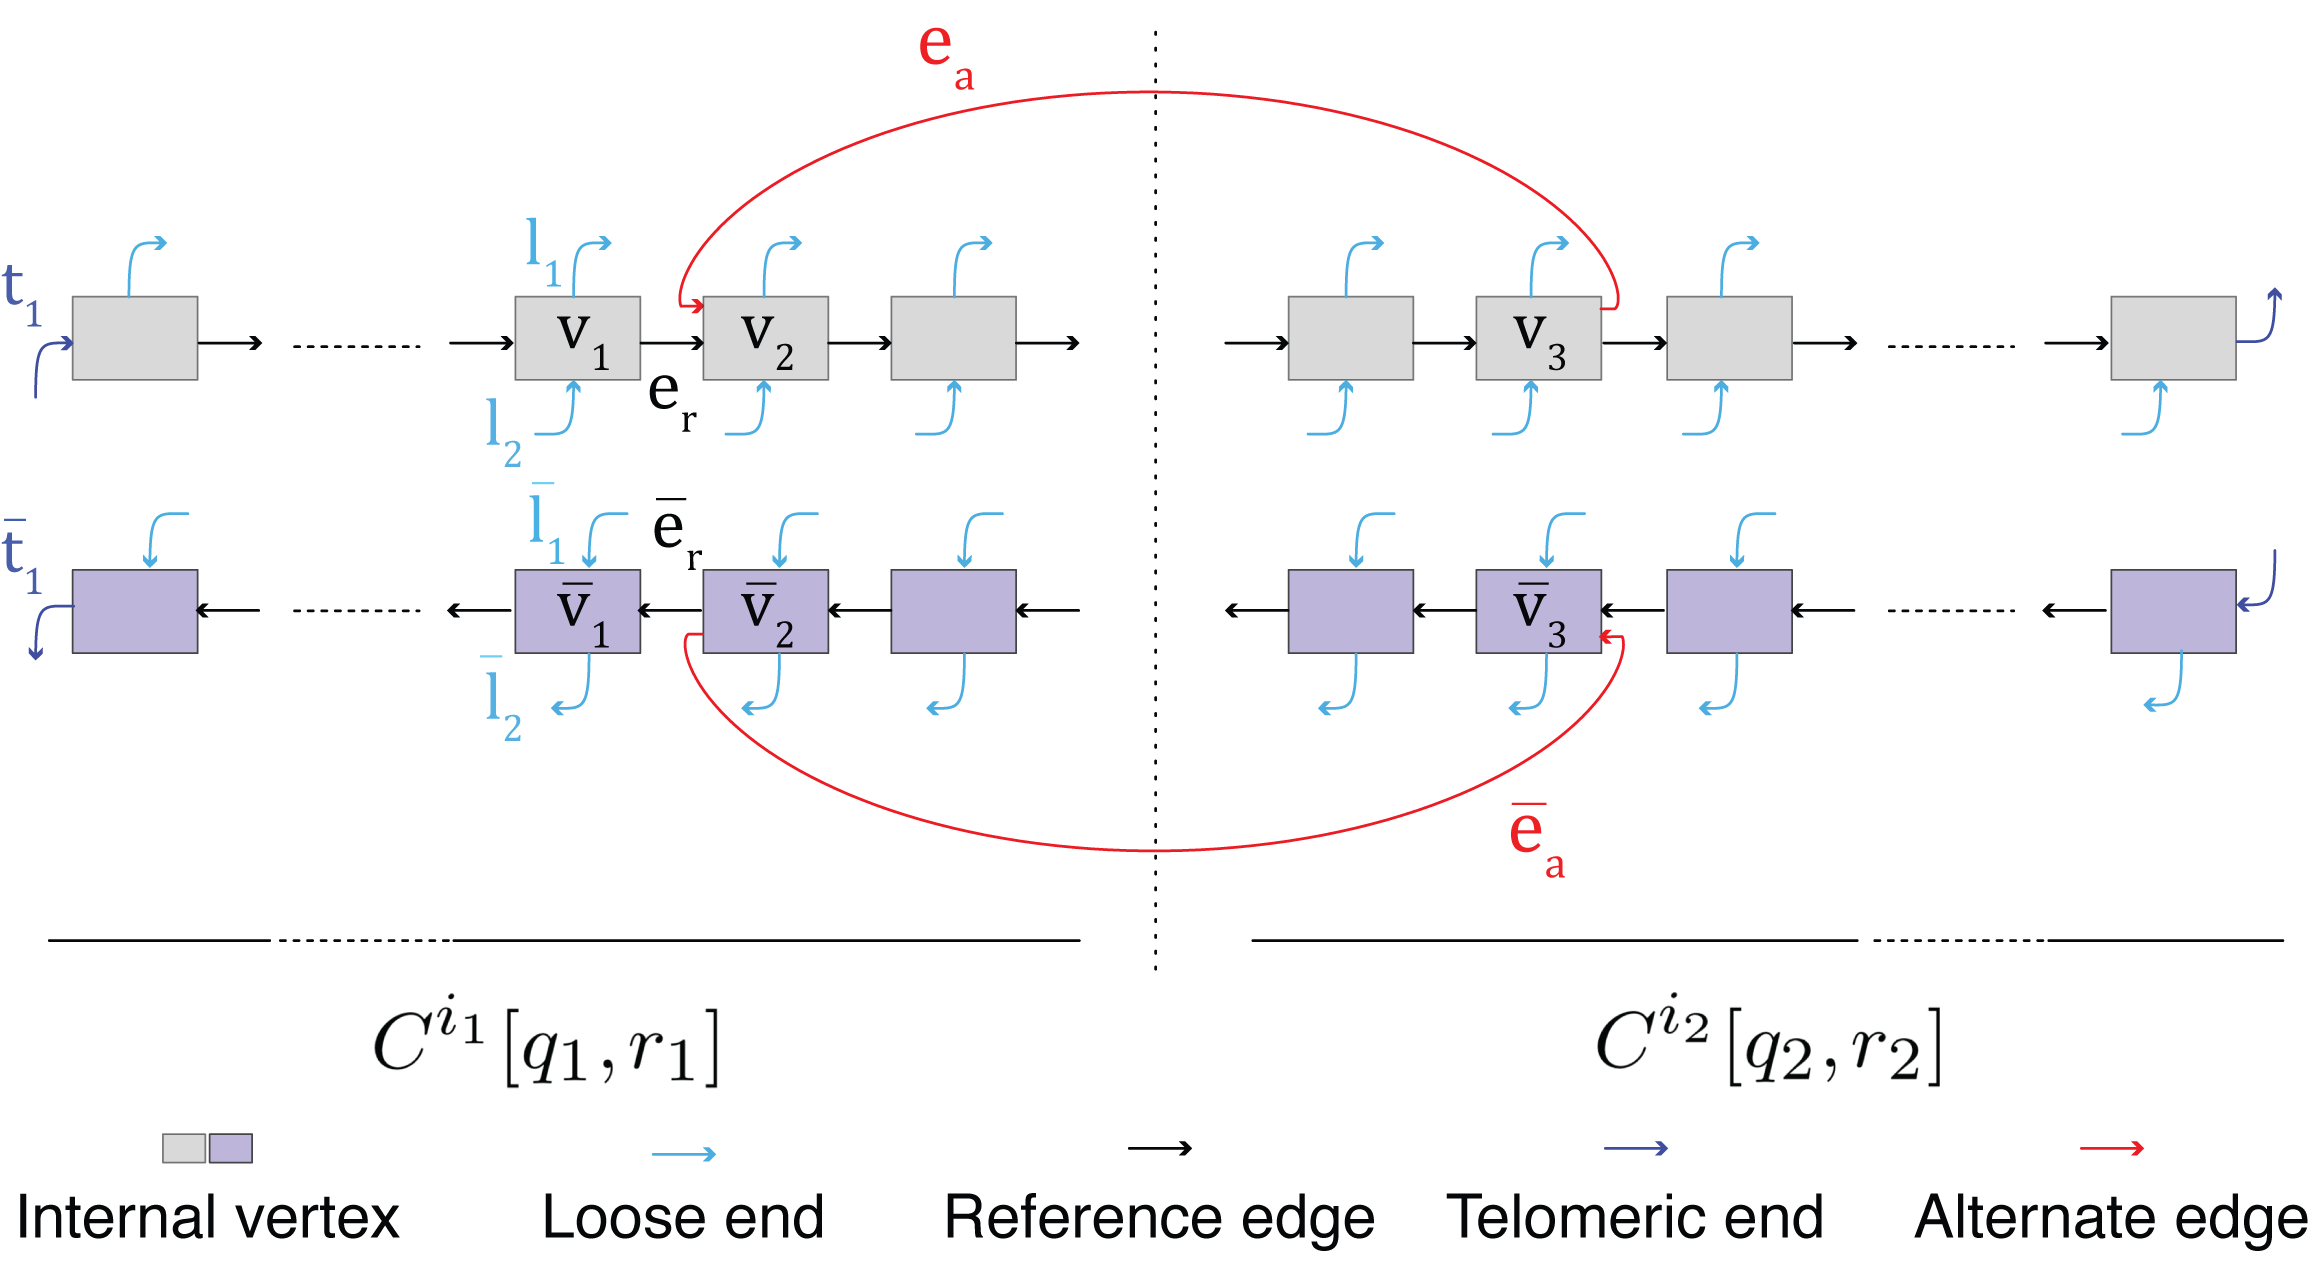
\includegraphics[width=0.95\linewidth]{figures/600ppi/ggraph_schematic.png}
    \caption{Schematic of a genome graph}
    \label{fig:ggraph_schematic}
\end{figure}

Because the phosphodiester bonds are always connecting the outgoing (3') end of a source vertex $v_1 = C^{i_1}[q_1,r_1]$ and the receiving (5') end of a sink vertex $v_2 = C^{i_2}[q_2,r_2]$, we can denote the genomic location of an edge $e = (v_1, v_2)$ with a tuple of the connected breakends $e = (b_o(v_1), b_r(v_2))$. For a node $v$ we name the set of incoming edges to its 5' end $E_{-}(v)$ and the set of outgoing edges from its 3' end $E_{+}(v)$.

Following this definition, there are at least two types of edges. The first type, \textit{REF} edges are the ones that are connecting breakends adjacent in the reference genome hence always with location $e_r = (C^{i}_{q}, C^{i}_{q + 1})$, if $i>0$, or $(C^{i}_{q_1 + 1}, C^{i}_{q_1})$, if $i<0, q \in [1,L_i)$. In contrast, the second type \textit{ALT} edges are neo-adjacencies that are not present in the reference genome and resulting from rearrangements (\textbf{Figure \ref{fig:ggraph_schematic}}).

Like a reverse complement pair of vertices $\{v, \bar{v}\}$ compose a double-stranded DNA segment, a reverse complement pair of edges $\{e, \bar{e}\}$ compose a \textit{junction}. Trivially, $e$ and $\bar{e}$ will always be the same type of edge, so we also have two types of junctions, REF and ALT. Each junction $a = \{e, \bar{e}\}, v_1 = C^{i_1}[q_1,r_1], v_2 = C^{i_2}[q_2,r_2]$ can be represented with the two breakends it connects, namely $b_1 = \{b_o(v_1), b_r(\bar{v_1})\} = C^{i_1}_{q_1 [1-I(i_1)] + r_1 I(i_1)}$, and similarly $b_2 = C^{i_2}_{q_2 [1-I(i_2)] + r_2 I(i_2)}$, where indicator function $I:\mathbb{R}\rightarrow \{0, 1\}, I(x)=1, if x \ge 0, I(x) = 0, if x<0$.

\begin{figure}[h!]
    \centering
    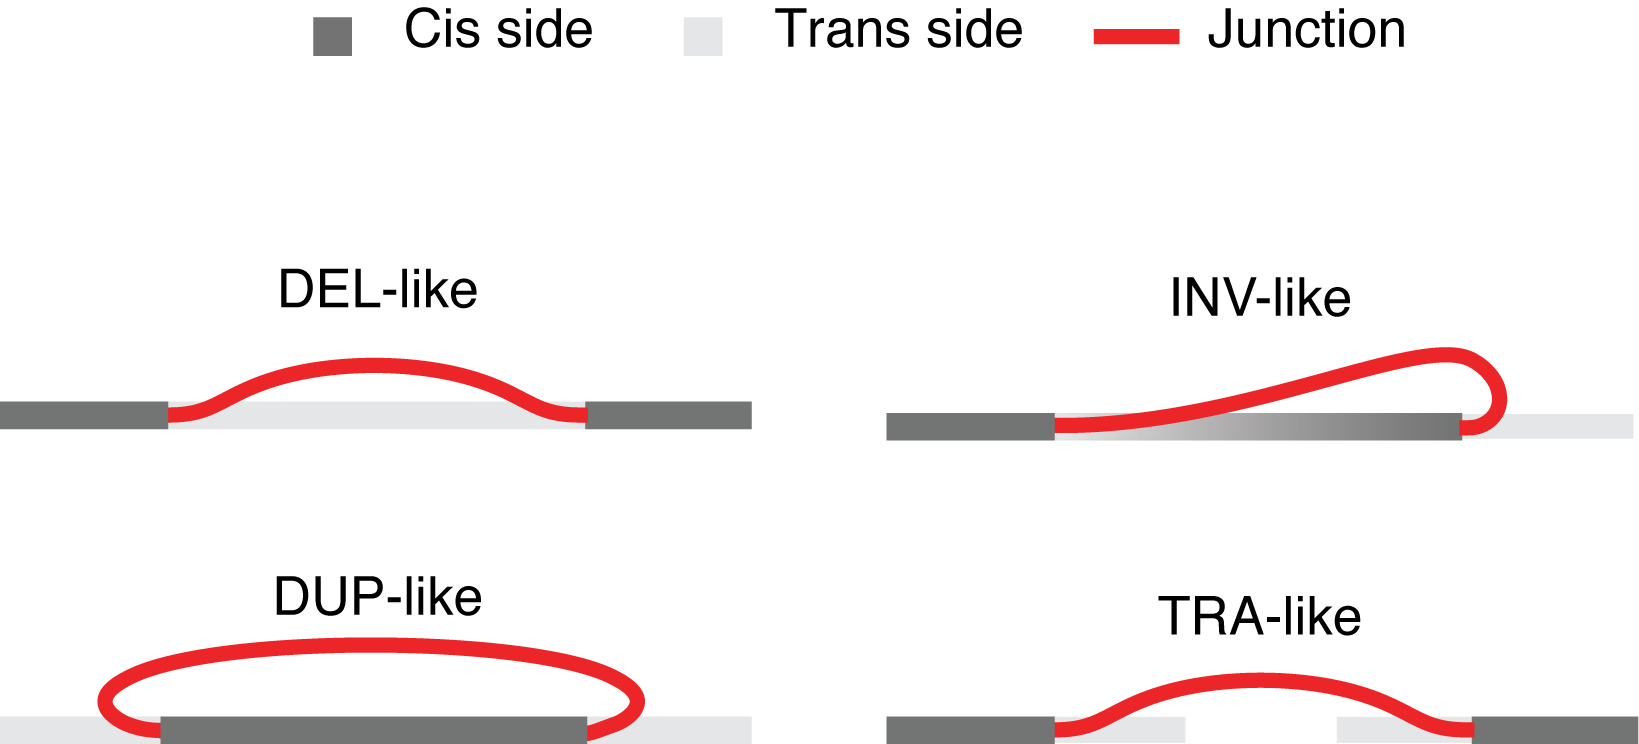
\includegraphics[width=0.95\linewidth]{figures/600ppi/junction_orientation.png}
    \caption{\textbf{Four basic classes of junctions.}}{Dark gray indicates the \textit{cis} side and light gray the \textit{trans} side of a breakend.}
    \label{fig:junction_orientations}
\end{figure}

For a breakend location in the middle of a chromosome, only one of its two sides is incident to the junction, we call this side the \textit{cis} side for it is the part of the genome that will be on the derivative molecule after introducing the junction, and the other \textit{trans} side. Based on the relative locations and orientations of its two connected breakends, we can classify a junction into four basic classes (\textbf{Figure \ref{fig:junction_orientations}}): DUP-like (tandem duplication), DEL-like (deletion), INV-like (inversion), TRA-like (translocation), named after the most common and simplest SV events that can give rise to such junctions. In WGS studies, these junctions are the direct products of SV calling methods like SvABA \cite{Wala2018-qa}, GRIDSS \cite{Cameron2017-pz}, Delly \cite{Rausch2012-ly}, Lumpy \cite{Layer2014-xq}, and many more. In the following section we show a basic algorithm to build a genome graph from a set of breakends and junctions.

% TODO!!!
\subsection{Build genome graph from breakends and junctions}
To describe a rearranged and copy number altered reference genome, we partition $\mathcal{C}$ according to a collection of \textit{breakends} $\mathcal{B}$. We also define a set of \textit{junctions} $\mathcal{A}$ representing alternative adjacencies between a set of the breakends in $\mathcal{B}$.




% TODO!!!
Each $b^i = C^ \in \mathcal{B},\ i \in 1,\ldots,c$ is an ordered and unique sequence of integer coordinates $B^i = (B^i_k), 1 \le B^i_k \le L_i$ on chromosome $i$, where $B^i_1$ = 1 and $B^i_{|B^i|} = L^i$.  Each junction $A \in \mathcal{A}$ is a tuple $(i_1,r_1,i_2,r_2),\ r_1 \in B^{|i_1|}, r_2 \in B^{|i_2|}$, $|i_1|, |i_2| \in  1, \ldots, c$ representing a (3'-5' phosphodiester) bond between the position $r_1 + \frac{-sgn(i_1)+1}{2}$ on chromosome / strand $C^{i_1}$ and position $r_2+\frac{sgn(i_2)+1}{2}$ on chromosome / strand $C^{i_2}$.  For every adjacency $A = (i_1,r_1,i_2,r_2) \in \mathcal{A}$ we require $\mathcal{A}$ to contain the reverse complement adjacency $\bar{A} = (-i_2,r_2, -i_1,r_1)$. The adjacencies in $\mathcal{A}$ are "alternative" relative to a set of "reference adjacencies" $\mathcal{R}$ implied by $B^i$, comprising tuples $(i, B^i_k, i, B^i_k)$ and $(-i, B^i_k, -i, B^i_k)$ for each breakend $B^i_k, k\in 1,\dots,|B^i|$ in each chromosome $i \in 1,\ldots,c$.



\begin{algorithm}[h!] 
    \caption{BuildGraph} 
    \label{algo:buildgraph}  
    \begin{algorithmic}[1]
        \Procedure{BuildGraph}{$\mathcal{A}$, $\mathcal{B}$} \Comment{Returns genome graph $G = (V, E, \psi, \phi)$}
        \State $G \gets emptyGraph;\quad$ $\phi, \psi \gets emptyDictionary$
        \State $\mathcal{B} = \mathcal{B} \cup \ getBreakPoints(\mathcal{A})$ \Comment{Extract additional breakends from junctions in $\mathcal{A}$}
        \For{$B^i_k,\ k\in 1,\ldots,|B^i|-1,\ c \in 1,\ldots,|\mathcal{C}|/2$}
        \State $v, \bar{v} \gets newVertices(2, \psi, "I")$ \Comment{$newVertices$ updates $\psi$ to map $v$ and $\bar{v}$ to "I"}
        \State $\phi(v) = (i, B^i_k, B^i_{k+1}-1)$
        \State $\phi(\bar{v}) = (-i, B^i_k, B^i_{k+1}-1)$
        \State $l_1, \bar{l_1}, l_2, \bar{l_2} \gets newVertices(4, \psi, "L")$
        \State $e_1, \bar{e_1}, e_2, \bar{e_2} \gets newEdges(\{ (l_1, v), (\bar{v},\bar{l_1}), (v, l_2), (\bar{l_2},\bar{v}) \}, \psi, "L")$
        \State \algorithmicif\ $k = 1$ \ \algorithmicthen\ \ $\psi(\{l_1, e_1, \bar{l_1}, \bar{e_1} \}) \gets "T"$  \Comment{Label telomeric loose ends with "T"}
        \State \algorithmicif\ $k = |B^i|-1$ \ \algorithmicthen\ $\psi(\{l_2, e_2, \bar{l_2}, \bar{e_2} \}) \gets "T"$
        \State $V(G) \gets V(G) \cup  \{ v, \bar{v}, l_1, \bar{l_1}, l_2, \bar{l_2} \})$
        \State $E(G) \gets E(G) \cup  \{ e_1, \bar{e_1}, e_2, \bar{e_2} \})$
        \EndFor        
        \algstore{buildgraph}        
    \end{algorithmic}
\end{algorithm}

\newpage

\begin{algorithm}[h!]
    \begin{algorithmic}
        \algrestore{buildgraph}
        \State $\mathcal{R} = referenceAdjacencies(\mathcal{B})$  \Comment{Get implied reference adjacencies from breakends}
        % \State $\mathcal{A} = \mathcal{A} \cup \ reverseComplement(\mathcal{A})$  \Comment{Make sure $\mathcal{A}$ contains both forward and RC adjacencies} 
        \For{$A = (i_1,r_1,i_2,r_2) \in \mathcal{A} \cup \mathcal{R}$}
        \If{$sgn(i_1)>0$}
        \State $v_1 \gets getVertex(\{ \hat{v} \ | \ \phi(v) = (i_1, q, r_1+\frac{-sgn(i)+1}{2}), v \in V(G), q \in \mathbb{N}\}$)
        \Else
        \State $v_1 \gets getVertex(\{ \hat{v} \ | \ \phi(\hat{v}) = (i_1, r_1 + \frac{-sgn(i)+1}{2}, q), v \in V(G), q \in \mathbb{N}\})$
        \EndIf
        \If{$sgn(i_2)>0$}
        \State $v_2 \gets getVertex(\{ \hat{v} \ | \ \phi(v) = (i_2, r_2 + \frac{sgn(i_2)+1}{2}, q), v \in V(G), q \in \mathbb{N}\})$
        \Else
        \State $v_2 \gets getVertex(\{ \hat{v} \ | \ \phi(\hat{v}) = (i_2, q, r_2 + \frac{sgn(i_2)+1}{2}), v \in V(G), q \in \mathbb{N} \})$
        \EndIf
        \State \algorithmicif\ $A \in \mathcal{R}$ \algorithmicthen\ $e = newEdges((v_1, v_2), \psi, "R")$ \ \algorithmicelse \ $e = newEdges((v_1, v_2), \psi, "A")$
        \State $E(G) \gets E(G) \cup \{e\}$
        \EndFor
        \State \textbf{return} $(V(G), E(G), \psi, \phi)$
        \EndProcedure
    \end{algorithmic}
\end{algorithm}

\newpage

\subsection{Walks on a genome graph map to rearranged karyotype}
Analogous to an assembly graph, on genome graph $G$, traveling through a walk $h = (v_1, e_1, v_2, e_2, \dots, e_{k-1}, v_k), k \in \mathbb{N^+}$, where each edge $e_i = (v_i, v_{i+1}), i \in 1, 2, \dots, k-1$, is equivalent to generating a substring of DNA sequence, simply by concatening the reference sequences of the vertices. If some of the edges along the walk belong to ALT edges $E_{A}$, then the walk represents a possible derivative sequence resulted from the SVs that gave rise to these edges. Since $G$ is skew-symmetric, every walk $h$ has a reverse complement walk $\bar{h} = (\bar{v_k}, \bar{e_{k-1}}, \dots, \bar{e_2}, \bar{v_2}, \bar{e_1}, \bar{v_1})$. We also denote the number of times a walk $h$ travel through a node $v$ or an edge $e$ using $\delta : (V \cup E, H) \rightarrow \mathbb{N}$. Based on this definition, we have two important observations.

First, given a tuple of genomic intervals $(v_1, v_2, \dots, v_k)$ whose order implies sequential covalent bonding, we can easily produce a genome graph and represent the tuple as a walk on that graph, by filling in edges between each consecutive pair of intervals based on their corresponding incident breakends, then add the same for the reverse complement walk. For example, the edge joining $(v_1, v_2)$ should be $(b_o(v_1), b_r(v_2))$. This observation implicated that any DNA sequence, as long as it can be constructed from pasting substrings of the reference genome, can be converted to a walk and a genome graph.

Second, every interval has exactly one upstream neighbor (incident to its 5' breakend, except for the first interval), and one downstream neighbor (incident to its 3' breakend, except for the last interval), as genomic DNA is known to be linear. Thus, we can associate a walk with a non-negative integer $\kappa(h) \in \mathbb{N}$ as the multiplicity of such molecule present in a genome. Consequently, the graph arise from these walks must posses be \textit{junction balanced}, a property we are going to define in \nameref{sub:JBGG} the next subsection.

\subsection{Junction-balanced genome graph} \label{sub:JBGG}
We define a mapping $\kappa:\{V \cup E\}\rightarrow \mathbb{N}$ of non-negative integer copy number (CN) to vertices and edges of $G$, where $\kappa(v),v \in V$ and  $\kappa(e),e \in E$ represent the CN of vertex $v$ and edge $e$, respectively. For a graph $G = (V, E)$ that arise from the aforementioned procedure from a set of tuples of genomic intervals, the following junction balance constraint is always true:

\begin{equation} \label{eq:junction_balance_constraint}
    \kappa(v)= \sum_{e\in E^-(v)} \kappa(e) = \sum_{e\in E^+(v)} \kappa(e)
\end{equation}

This is because to travel into $v$ once one must travel through one of the edges in $E_{-}(v)$, and vice versa for the outgoing edges. In plain language, the principle of \textit{junction balance} constrains the CN of every vertex to be equal to the sum of its incoming edges and the sum of its outgoing edges. Formally,

\begin{equation} \label{eq:sum_of_walk}
    \begin{split}
        \forall v \in V, \kappa(v) = \sum_{h \in H}\kappa(h)\delta(h, v) \\
        \forall e \in E, \kappa(e) = \sum_{h \in H}\kappa(h)\delta(h, e)
    \end{split}
\end{equation}

in which $\delta: \{H, V \cup E\} \rightarrow \mathbb{N}$ is the number of times $h$ travels through a vertex or an edge $\sum_{j \in 1,\dots,k}I(v = v_j)$, with the only exception that if $h = (v_1, e_1, v_2, e_2, \dots, e_{k-1}, v_k), v_1=v_k, k \in \mathbb{N^+}$ is circular $\delta(h,v_k) = 0$, so that $v_k$ is not double counted.

In addition, since double-stranded DNA require both strands to have the same CN, we require the CN $\kappa$ to obey \textit{skew-symmetry}, which means that every vertex or edge must have the same copy number as its reverse complement.

\begin{equation} \label{eq:skew_symmetry}
    \kappa(v) = \kappa(\bar{v}),\ \forall_{v \in V} \quad \kappa(e) = \kappa(\bar{e}),\ \forall_{e \in E}
\end{equation}

We call the combination $(G,\kappa)$ for which $\kappa$ satisfies Eqs. \ref{eq:junction_balance_constraint}-\ref{eq:skew_symmetry} a \textit{junction-balanced genome graph} (JBGG).

% TODO!!!
% Flow decomposition:
% Why is a complete graph contain all the possible walks from source to sink?
\subsection{Decomposing a JBGG to walks}
In a perfect scenario where we have infinitely long sequencing reads, we can read out any sequence directly and fully (telomere to telomere), for any rearranged karyotype. However, in practice, sequencing reads from existing technologies are fragmented and limited in length, so the walks representing complete and true karyotypes are always latent. Despite current long-read sequencing provides us a better chance at obtaining the rearranged allele, it is still "local" relative to the scale of some of the most long-range complex SV events like tyfonas \cite{Hadi2020-um} (see also Chapter \ref{chap:complex_events}). Furthermore, due to the differences in cost, accuracy, throughput, and analytical robustness, the overwhelming majority of cancer WGS data is still based on massive parallel short-read sequencing, with which SV events are detected as copy number aberrations and junctions. Despite certain challenges, for instance with SVs in repetitive regions, short-read WGS has been found to approach the complete SV repertoire well \cite{Behr2021-gf}.

% TODO!!!: why a complete genome graph contains all possible karyotypes
Though we cannot directly read the derivative sequence after rearrangement, from junctions we can always build a genome graph (see \nameref{algo:buildgraph} in later sections). If we have the complete knowledge on all junctions, then this graph will encapsulate every possible karyotype that could result from them, hence must contain the set of walks representing the true sequence (proof not shown). The enumeration of all possible walks from all the source nodes to all the sink nodes is analogous to elementary flux mode of a stoichiometric matrix \cite{Maarleveld2013}, and produces a set of paths and cycles $H$ where the latter can be further embedded to form more complex walks.

However, such genome graphs only deal with the topology of junctions, and for a coherent double-stranded DNA model, the vertices and edges' dosages need also be constrained by Eq. \ref{eq:junction_balance_constraint} and Eq. \ref{eq:skew_symmetry}. With that we can define the reverse problem of Eq. \ref{eq:sum_of_walk},



\begin{equation} \label{eq:walk_decomposition}
    \begin{aligned}
        \text{Given } & G = (V, E), \kappa(G) \\
        \text{find } & \kappa(h):H \rightarrow \mathbb{N} \\
        s.t. & \forall v \in V, \kappa(v) = \sum_{h \in H}\delta(h,v)\kappa(h) \\
        & \forall e \in E, \kappa(e) = \sum_{h \in H}\delta(h,e)\kappa(h) \\
        & \kappa(h) = \kappa(\bar{h})
    \end{aligned}
\end{equation}

%Suppose we are given an input JBGG with its junction-balanced CN $G, \kappa(G)$, the walk decomposition problem is now to find a multiplicity of every walk $\kappa(h), h \in H$, such that Eq. \ref{eq:sum_of_walk} is satisfied. 
Since in its essence, this is equivalent to a flow decomposition problem, the junction balance constraints \ref{eq:junction_balance_constraint} guarantee that it is feasible, usually with a huge number of possible solutions. Upon this pool of possible karyotypes, we can further define different loss functions, such as parsimony (number of unique walks with $\kappa(h)>0$), to reach some optimal guesses at what the actual rearranged allele is that constitute the input JBGG. Taking the most naive formulation as an example, to minimize the total number of unique walks to reconstitute an input JBGG, formally the question is defined as,

\begin{equation} \label{eq:walk_decomposition_parsimony}
    \begin{aligned}
        \text{Given a JBGG } & G = (V, E), \kappa(G) \\
        \underset{\kappa(h):H \rightarrow \mathbb{N}}{\text{minimize}} & \sum_{h \in H} [\![ \kappa(h) ]\!] \\
        s.t. & \forall v \in V, \kappa(v) = \sum_{h \in H}\delta(h,v)\kappa(h) \\
        & \forall e \in E, \kappa(e) = \sum_{h \in H}\delta(h,e)\kappa(h) \\
        & \kappa(h) = \kappa(\bar{h})
    \end{aligned}
\end{equation}


We shall see an example of solving a variation of this problem in \ref{chap:tel_crisis}.

When combined with read coverage data, we can further infer JBGG by filling in an optimal set of CNs for all the vertices and edges. We call this problem the inference or \textit{reconstruction of JBGG}, to which we will present one solution in the next section.

% Intuitively, all SVs except for whole chromosome/genome duplications or episomal amplifications result in the breakage of DNA and forming breakends. When new phosphodiester bonds form, there must be two breakends .

%  For lack of better alternative, most early cancer SV studies hitherto treat these two facets of the same rearranged sequence separately or informally combine them to describe certain patterns \cite{stephens2011,baca2013}. The PCAWG consortium made fundamental effort to build up a pool of CNA and junction patterns for different classes of SV events, but still .... 

%===========================%
\section{Junction Balance Analysis infers copy numbers on genome graphs from short-read whole genome sequencing}

We developed an algorithm, JaBbA, to accurately infer junction-balanced genome graphs from WGS data. In the following three subsections, we will 1) formally define this algorithm \textit{junction balance analysis}, 2) describe the pipeline implementing the algorithm, and 3) comprehensively compare its features and performance to other methods of similar purpose.

%Analogous to previous approaches, we define a (directed) genome graph of vertices representing strands of genomic segments and edges  representing a pair of 3' and 5' DNA ends that are adjacent in the reference genome (REF edge) or connected through rearrangement (ALT edge). A \textit{junction balanced genome-graph} assigns every vertex and edge in the graph an integer CN, while enforcing the constraint that the dosage of every interval (vertex) is equal to the sum of the JCN of the incoming (or similarly, outgoing) junctions (\textbf{Fig. \ref{fig:jabba_io}}).  The MIP optimization solved by JaBbA minimizes the residual between observed read depth and inferred interval dosage through joint assignment of CN to intervals and junctions (\textbf{Fig. {fig:Fig1}B, Fig. {fig:S1}C}, sec:methods).

\subsection{Formulation of the mixed-integer quadratic programming problem}

\begin{figure}[!t]
    \centering
    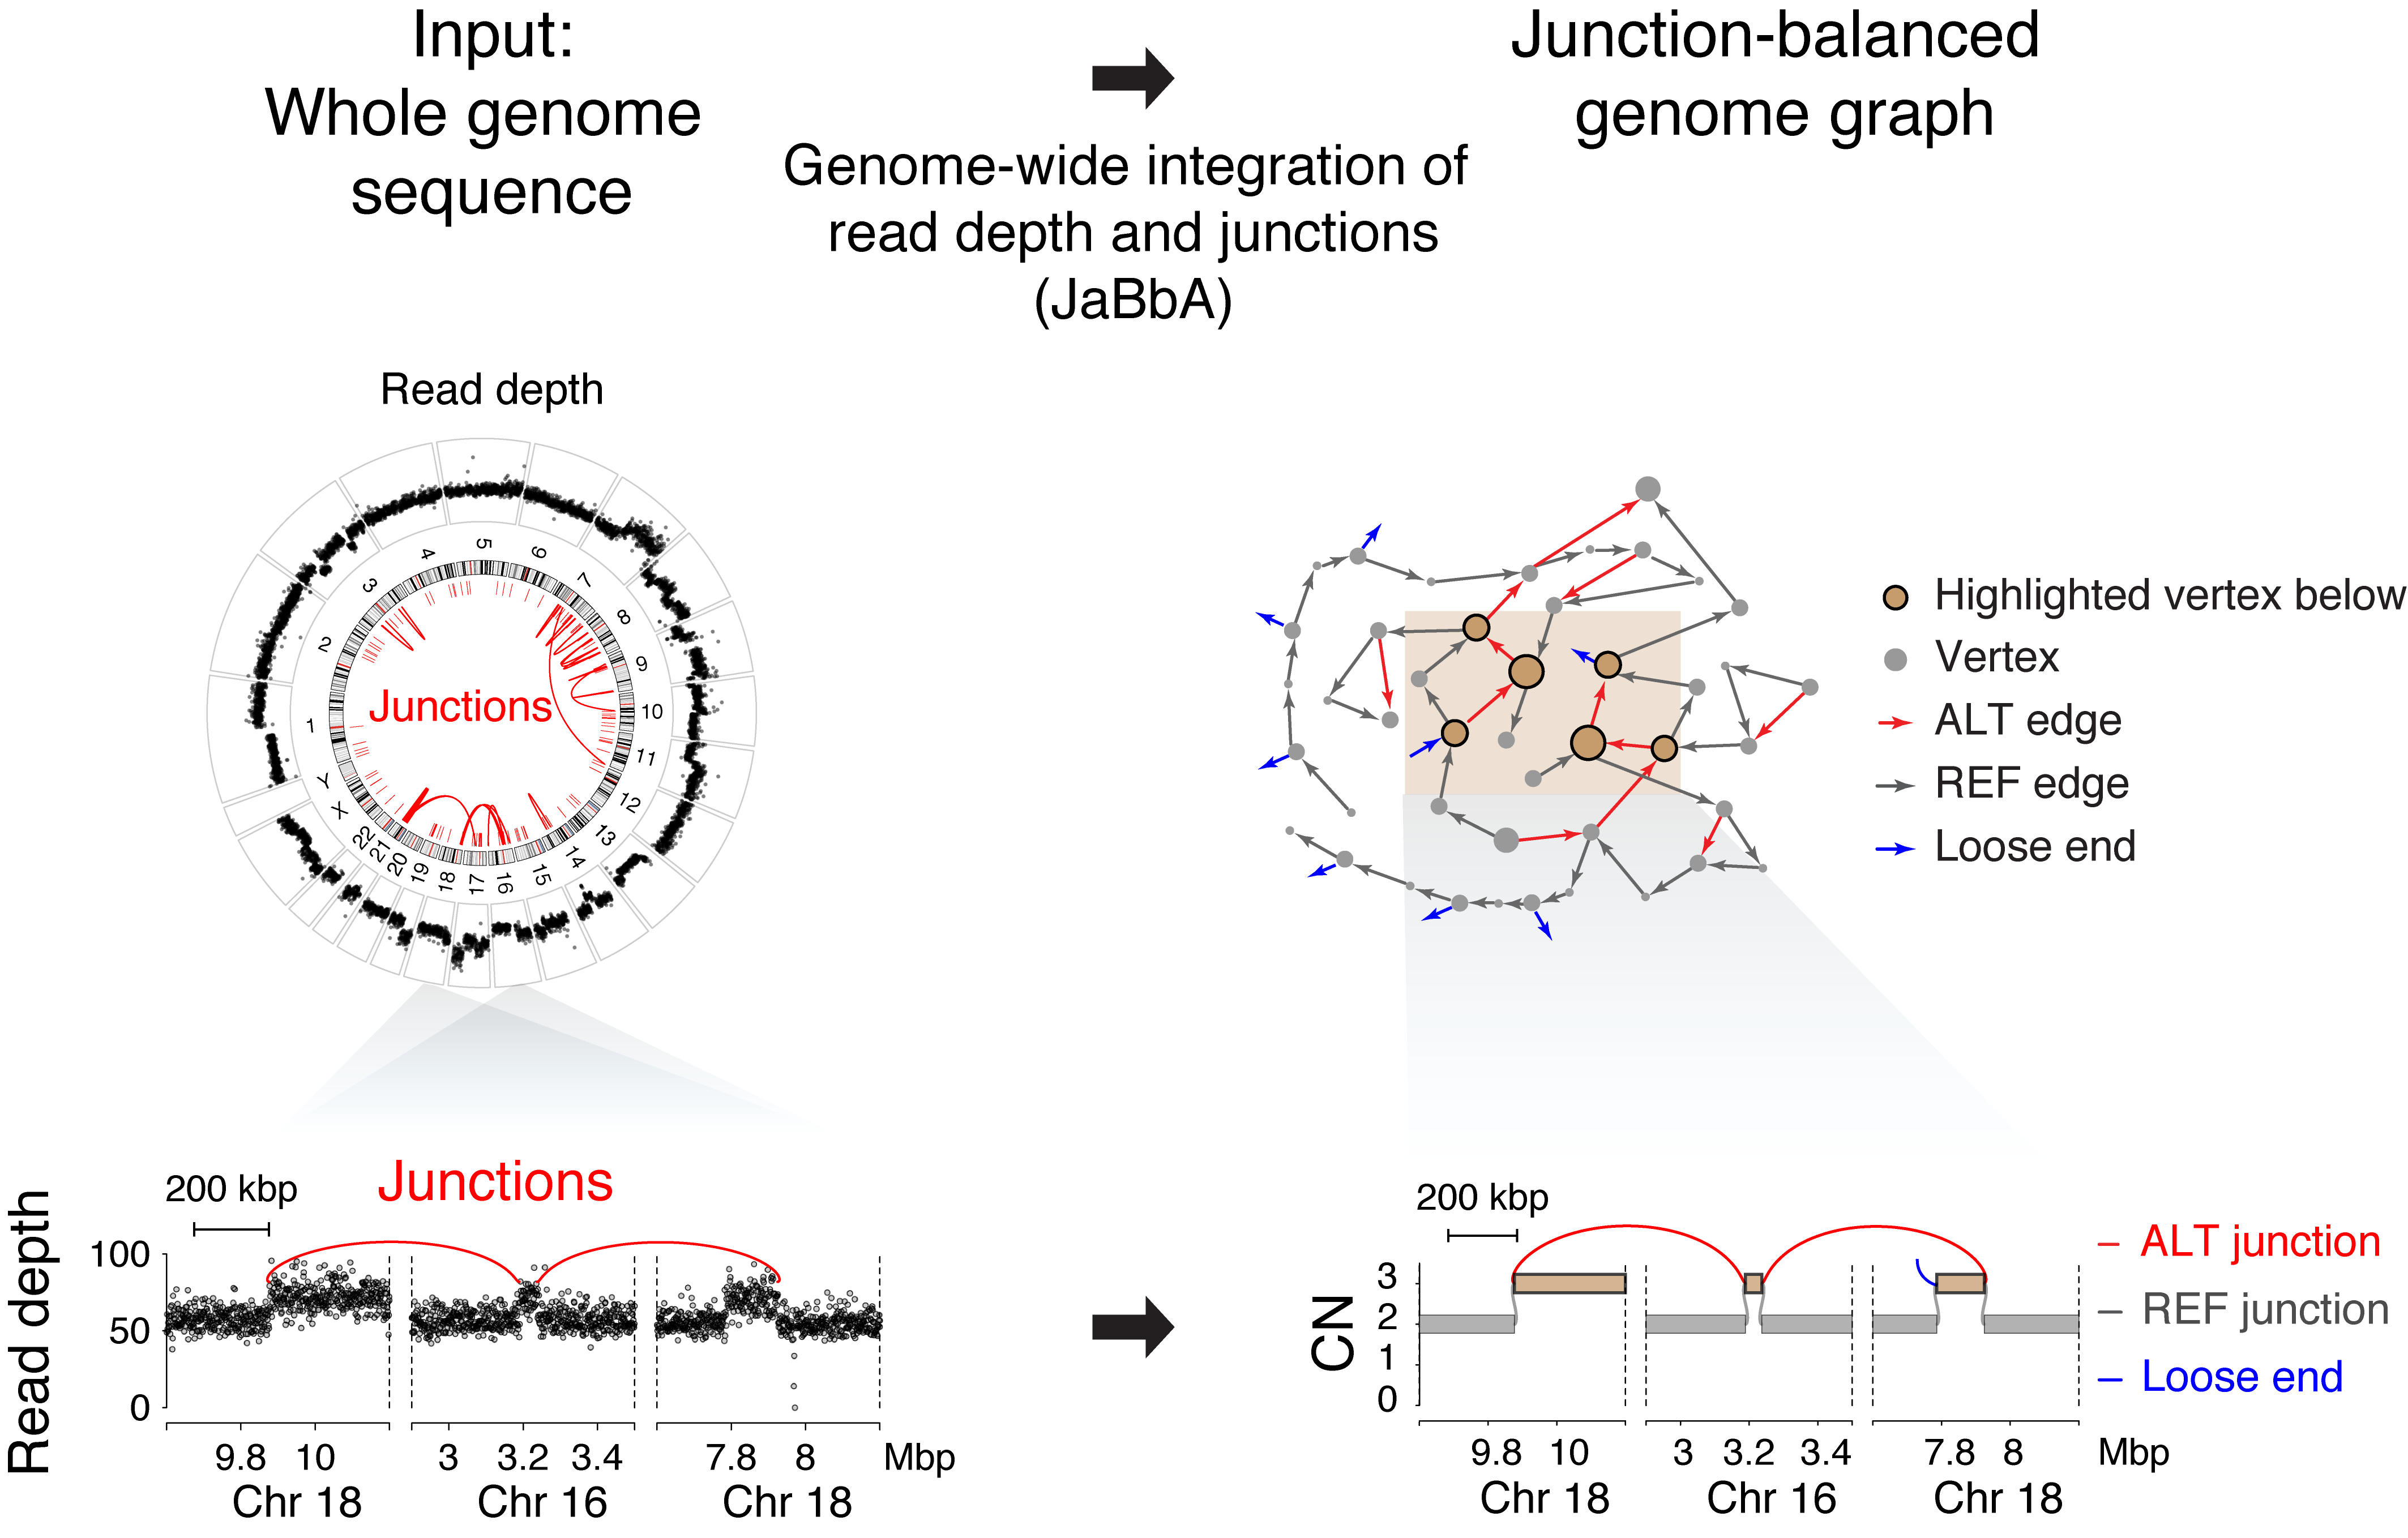
\includegraphics[width=0.95\linewidth]{figures/600ppi/jabba_io.png}
    \caption{\textbf{Inputs and outputs of Junction Balance Analysis} Top left, read depth on genomic bins and junctions are the two required input data summarized from a WGS. Bottom left, an example locus showing read depth as scatter plots over reference coordiantes and input junctions as red curves connecting the breakends. Top right, the network layout of the genome (sub)graph of the highlighted locus built from the junctions. Bottom right, the junction balanced genome graph (JBGG) output with integer CN for segments on the Y axis and junction CN implied.}
    \label{fig:jabba_io}
\end{figure}

% \subsubsection*{Inferring Junction Balanced Genome Graphs}
We infer JBGGs from a genome graph $G$ and binned, normalized, and purity / ploidy-transformed read depth data $x \in \mathbb{R}^n$ across $n$ genomic bins (see below for read depth transformation details)  through the solution of a mixed integer quadratic program (MIQP), which assigns an integer CN $\kappa:V_I \cup E \rightarrow \mathbb{N}$ to the vertices and edges of $G$.  The genome graph $G$ is generated, as above, from a set of breakends $\mathcal{B}_{seg}$ obtained from a preliminary segmentation of genome-wide read depth (i.e. via segmentation software such as CBS) and a set of junctions $\mathcal{A}$ (i.e. from a junction caller such as SvABA or DELLY).

Each vertex $v \in V_I(G)$ is associated with a partition of bins $J(v) \subseteq \{1, \ldots, n\}$ (based on genomic coordinate overlap) and a mean bin value $\rho(v) = \frac{1}{|J(v)|}\sum_{j \in J(v)} x_j$.  We model each bin subset $x_{J(v)}$ as an i.i.d. sample from a Gaussian distribution with standard deviation $\sigma(v)$ and mean $\kappa(v)$.  The log likelihood is

\begin{equation} \label{eq:nodeloglikelihood}
    log P(x_{J(v)} | \kappa(v), \sigma(v)) =  \sum_{j \in J(v)} log \ \mathcal{N}(x_j | \kappa(v), \sigma(v)^2) = - \mathcal{V}(v, \kappa, x, J) + Const(\kappa)
\end{equation}

where $\mathcal{N}(\mu, \sigma^2)$ is the Gaussian probability density function with mean $\mu$ and variance $\sigma^2$ and $\mathcal{V}(v, \kappa, x, J) =  \frac{|J(v)|}{2\sigma(v)^2}(\rho(v)- \kappa(v))^2$ is the \textit{read depth residual} of vertex $v$. The variance $\sigma^2(v)$ is a $\kappa$-independent parameter that models read depth noise and is computed directly from the data.  The simplest noise model is a constant, where this parameter is set to the genome-wide sample variance of the read depth around each vertex mean: $\sigma^2(v) = \hat{\sigma}^2 = \frac{1}{n-1} \sum_{v \in V_I} \sum_{j \in J(v)} (x_j - \rho(v))^2$.  In practice, we apply a vertex-specific variance estimate $\sigma^2(v)$ to account for heteroscedasticity in the read depth data (see "JaBbA model fitting" section below).

Given this model, the joint log-likelihood of the read depth data $x$ across the graph given copy number assignment $\kappa$ is
\begin{equation} \label{eq:jointloglikelihood}
    log P(x | \kappa) = - \sum_{v \in V_I} \mathcal{V}(v, \kappa, x, J) + Const(\kappa)
\end{equation}
We also refer to $V(G, \kappa, x, J) = \sum_{v\in V_I} V(v, \kappa(v), x, J)$ as the \textit{read depth residual} of the JBGG $(G, \kappa)$ relative to data $x$.

The satisfaction of junction balance and skew-symmetry constraints in Eq. \ref{eq:junction_balance_constraint}-\ref{eq:skew_symmetry} may place nonzero copy number at one or more loose end edges.   Each loose end in the input graph represents a slack variable that allows the junction balance constraint to be relaxed at specific internal vertices, allowing the data to be fit even when junctions are missing from the input (e.g. due to low mappability, sequencing depth, or purity).  Only loose ends that are given nonzero CN, are considered to be "used" in the final graph. To penalize solutions that require the use of many loose ends, we add an exponential prior with decay parameter $\lambda$ on the loose end CN in $(G, \kappa)$, which makes models with many missing junctions unlikely.  This prior has log likelihood

\begin{equation} \label{eq:looseendpenalty}
    log P(\kappa | G, \lambda) = -|V_I|log\lambda - \lambda \mathcal{R}(G, \kappa)
\end{equation}
where
\begin{equation} \label{eq:complexitypenalty}
    \mathcal{R}(G, \kappa) = \sum_{v \in V_I} \mathcal{R}(v, \kappa) = \sum_{v \in V_I} \kappa(E_L^-(v))  + \kappa(E_L^+(v))
\end{equation}

is a \textit{complexity penalty}. Adding the log likelihood in  Eq. \ref{eq:jointloglikelihood} to the prior in Eq. \ref{eq:looseendpenalty} yields a penalized log likelihood for the data with regularization parameter $\lambda$. Under this model, the maximum a posteriori probability (MAP) estimate of $\kappa$

\begin{equation} \label{eq:objectivefunction}
    f(G, \kappa, x, J, \lambda) = \mathcal{V}(G,\kappa, x, J) + \lambda \mathcal{R}(G, \kappa)
\end{equation}

which combines the quadratic read depth residual $\mathcal{V}$ and $\ell_1$-norm  complexity penalty $\mathcal{R}$ into a single quadratic objective.   In practice, we apply models that penalize the number of loose ends with nonzero copy number, i.e. applying an $\ell_0$-norm penalty  $\mathcal{R}(\kappa) = \sum_{v \in V_I} [\kappa(E_L^-(v))>0]  + [(\kappa(E_L^+(v))>0])$.  We use $f$ to define a MIQP, which we solve to infer a MAP estimate for $\kappa$ given data $x$ and genome graph $G$:

\begin{equation} \label{eq:MIQP}
    \begin{aligned}
         & \underset{\kappa: V_I \cup E \rightarrow \mathbb{N}}{\text{minimize}}
         &                                                                       & f(G, \kappa, x, J, \lambda)                                                                                                                               \\
         & \text{subject to}
         &                                                                       & \kappa(v) = \kappa(\bar{v}),\ \forall_{v \in V_I}                                                                                                         \\
         &                                                                       &                                                   & \kappa(e) = \kappa(\bar{e}),\ \forall_{e \in E}                                                       \\
         &                                                                       &                                                   & \kappa(v)= \sum_{e\in E^-(v)} \kappa(e)         & = \sum_{e\in E^+(v)} \kappa(e), \forall_{v \in V_I} \\
    \end{aligned}
\end{equation}

The resulting MAP estimate $\hat{\kappa}$ defines the JBGG $(G,\hat{\kappa})$ which is outputted and returned to the user.


\subsection{JaBbA pipeline}
Overall, the pipeline can be split into 3 parts, 1) building a primitive genome graph from the primary segmentation of coverage, 2) fitting integer CN for vertices and edges by solving the MIQP problem, and 3) simplify the output graph and report in the form of gGraph of gGnome package (see section \ref{sec:implement_ggnome}).

Junction Balance Analysis (JaBbA, \url{https://github.com/mskilab/JaBbA}) is an R package freely available under the MIT license. The required inputs to JaBbA are binned (e.g. 200bp) and normalized read depth data $y$, purity $\alpha$, ploidy $\tau$, a set of junctions $\mathcal{A}$ (see mathematical formulation above), and a hyperparameter $\lambda$. The key output is a \texttt{gGraph} object representing a junction-balanced genome graph (i.e. solution to \textbf{Eq. \ref{eq:MIQP}}) which can be queried and analyzed using downstream algorithms, e.g. SV event classification algorithms in the \texttt{gGnome} package (\url{https://github.com/mskilab/gGnome}, see "Structural variant event classification" section below). The workflow of JaBbA is composed of four phases: read depth preprocessing, graph building, JaBbA model fitting, and postprocessing.

\subsubsection*{Read coverage preprocessing, primary segmentation, and purity-ploidy estimation}
Raw input read depth data are generated for tumor and matched normal (i.e. constitutional) samples by tallying the count of midpoints of well aligned (MAPQ $>$ 0) proper read pairs in a vector $z \in \mathbb{Z}^n_+$ (e.g. $n \approx$ 15 million for 200 bp bins across hg19).  These are further GC-corrected and mappability normalized through an iterative LOESS fitting procedure similar to \cite{Ha:2012kr} and implemented in the fragCounter R package (https://github.com/mskilab/fragCounter). Briefly, a local estimated scatterplot smoothing (LOESS) function $f_{GC}$ is fitted (R \ttt{stats} package \ttt{loess} function) to a random (100,000) subsample of bins to predict read depth as a function of GC content. Each bin's read depth $z_j,~j \in \{1, ... n\}$ is then divided by its fitted value $f_{GC}(z_j)$ to yield the normalized value $z^{GC}_j$.  A similar LOESS-based procedure is then applied to correct each GC-corrected read depth $z^{GC}_j$ with respect to its 100mer mappability score to yield the GC and mappability corrected read depth $z^{GCM}_j$.  This procedure is applied separately for tumor and matched normal (if applicable).

The ratio of the GC and mappability corrected read depth profiles for the tumor $z^T$ and normal $z^N$ is then used to derive the normalized read depth profile $y \in \mathbb{R}^n_+$ where $y_j = \frac{z_j^Tm_j^N}{z_j^N},~j \in \{1, ... n\}$ and $m^N_j$ is the chromosomal-wide median in the normal read depth data for the chromosome containing bin $j$.  Correction of the tumor / normal ratio by $m^N_j$ maintains a linear relationship between read depth and locus abundance in the original sample. Without this final step, bins from the X and Y chromosomes in a diploid male tumor will show the same read depth as the autosomes.  Samples without a matched normal (e.g. cell lines) are divided by a "universal" (i.e. average) normal averaged across 943 GC and mappability corrected TCGA normal read depth profiles and then chromosome balanced.


We note that the read depth normalizations, described above, are formally performed upstream of the JaBbA pipeline (e.g. via fragCounter, R / Bioconductor). The goal of these normalizations is to reduce biases, with the goal of rendering the binned read depth $y_j$ proportional (± noise) to the abundance of locus $j$ in the tumor sample (which may include admixed normal cells).  The final (purity / ploidy) transformation, included formally as part of the JaBbA pipeline, will renders the normalized read depth approximately equal (± noise) to its clonal integer CN in the tumor (given an accurate purity / ploidy estimate). Given a tumor sample with purity $\alpha \in [0, 1]$, ploidy $\tau \in \mathbb{R}_+$, and normalized read depth data $y$, the read depth $y_j$, tumor CN $\kappa(j)$, and constitutional CN $\kappa_N(j)$ will obey:

\begin{equation} \label{eq:ppbins}
    \frac{y_j}{\sum_{\hat{j} = 1}^n y_{\hat{j}}} \approx \frac{\alpha \kappa(j) + (1-\alpha)\kappa_N(j)}{\sum_{\hat{j} = 1}^n \alpha \kappa(\hat{j}) + (1-\alpha)\kappa_N(\hat{j})}
\end{equation}

Given $\bar{y} = \frac{1}{n}\sum_{\hat{j} = 1}^{n} y_{\hat{j}}$, $\tau \approx \frac{1}{n}\sum_{\hat{j} = 1}^{n} \kappa(\hat{j})$, and a near diploid constitutional sample (i.e. in which $\frac{1}{n}\sum_{\hat{j} = 1}^{n} \kappa_N(\hat{j}) \approx 2$),

\begin{equation} \label{eq:ppbins2}
    y_j \approx \frac{\alpha\kappa(j) + (1-\alpha)\kappa_N(j)}{\alpha \tau + 2(1-\alpha)} \bar{y}
\end{equation}

Defining

\begin{equation} \label{eq:purityploidycorrection}
    \begin{split}
        \beta = \frac{\bar{y}\alpha}{\alpha\tau+2(1-\alpha)} \\
        \gamma = \frac{2\bar{y}(1-\alpha)}{\alpha\tau+2(1-\alpha)}
    \end{split}
\end{equation}

yields the following equation:

\begin{equation} \label{eq:ppbins3}
    \kappa(j) \approx x_j = \frac{2y_j - \kappa_N(j)\gamma}{2\beta}
\end{equation}

Given known constitutional copy number (in practice, $\kappa_N(j) = 2$ for all bins with the exception of X and Y chromosome in males, where $\kappa_N(j) = 1$), the right hand side of Eq. \ref{eq:ppbins3} is computed directly from the (GC and mappability corrected, tumor / normal ratio transformed) read depth data, purity, and ploidy and represents the binned read depth input $x$ to JaBbA.

\subsubsection*{Graph building}
To build the genome graph $G$, the binned read depth $x$ is segmented (e.g. using CBS) to yield the breakends $\mathcal{B}$.  These breakends are combined via \textbf{Algorithm \ref{algo:buildgraph}} with the junctions $\mathcal{A}$ to yield $G$.  Briefly, this procedure 1) divides the reference genome into internal vertices $v_I \in V_I$ each of which will be assumed to have a coherent CN, and 2) establishes edges $e \in E=E_{R} \cup E_{A} \cup E_{L}$ that each represents an adjacency consistent with the reference genome (REF edge, $E_R$), created by an rearrangement junction (ALT edge, $E_A$), or an unmatched breakend (loose end, $E_L$). The ends of the vertices are the union of junction breakends $getBreakPoints(\mathcal{A})$ and a primary segmentation of the genome $\mathcal{B}_{seg}$ using the Circular Binary Segmentation algorithm \cite{olshen2004} (CBS), or from user input.  The mapping $J(v)$ (see above) is constructed to associate internal vertices $v \in V_I(G)$ with partitions of bin indices.



\subsubsection*{JaBbA model fitting}
Given a genome graph $G$ and GC / mappability corrected, normalized, purity / ploidy transformed read depth data $x \in \mathbb{R}^n$, and bin set $J(v) \subseteq \{1, \ldots, n\},~v \in V_I(G)$ , we infer a junction balanced genome graph $(G, \kappa)$ using the procedure outlined above ("Inferring junction-balanced genome graphs" section) with the following modifications:  Instead of the arithmetic mean $\rho(v)$, we use the sample geometric mean $\rho(v) = exp(\frac{1}{|J(v)|}\sum_{j \in J(v)} ln(x_j))$, which is more robust to outliers.  To model heteroscedasticity in read depth, we compute a vertex specific variance function $\sigma^2(v)$. Specifically, we use LOESS to fit a smooth non-linear function $f$ that links copy number to variance by fitting the sample mean $\rho(v)$ and sample variance  $\hat{\sigma}^2(v) = \frac{1}{|J(v)|-1} \sum_{x \in J(v)} (x_j - \rho(v))^2$ across all $v \in V_I$.  This function is then used to determine the segment-specific variance term as $\sigma^2(v) = f(\rho(v))$.  These $\sigma^2(v)$ values are then used to populate the read depth residual sum of squares $\mathcal{V}(v, \kappa, x, J)$ portion of the objective function in \textbf{Eq. \ref{eq:nodeloglikelihood}}. Combining with the user-defined loose end penalty hyperparameter $\lambda$ (default 100, tuned for 200 bp binned tumor / normal pairs, see above), the MIQP problem (\textbf{Eq. \ref{eq:MIQP}}) is solved on the genome graph using an $\ell_0$ complexity penalty. The solver is \texttt{CPLEX} (v12.6.2, IBM).

To increase sensitivity for missed junctions, the JaBbA pipeline employs several iterations of MIQP inference when two tiers of junctions (high and low confidence) are provided.  Briefly, we fit a model using only high-confidence (e.g. FILTER=PASS in the unfiltered \texttt{SvABA} output VCF) junctions as input.  In subsequent iterations, we fit a modified model that includes additional low-confidence junctions (e.g. those with low read support) that occur near (<1 kbp) a loose end in the previous iteration.  This procedure is run for a maximum of four iterations, or until no additional low confidence junctions near loose ends from the previous iteration have been found.   Such a procedure particularly improves junction sensitivity in the setting of low purity and / or read depth.

% \subsubsection*{Graph partitioning}


\subsubsection*{Post processing and allelic CN fitting}
After the optimization with \texttt{CPLEX}, we further simplify the solution by merging neighboring vertices of the same total CN that are connected only through REF edges. If ALT and REF read counts at constitutional heterozygous SNP sites are provided as (optional) input to JaBbA, we also infer the tumor allelic CN $\kappa_{h}(v)$ and  $\kappa_{l}(v)$ corresponding to the "high" ($h$) and "low" ($l$) allele, where  $\kappa_{h}(v) + \kappa_{l}(v) = \kappa(v)$ and $\kappa_{l}(v) \le \kappa_{h}(v)$, for each internal vertex $v \in V_I$ that overlaps a heterozygous SNP.  (Only biallelic heterozygous SNPs with two constitutional states, i.e. ALT and REF are considered.)

Briefly, we model the "low" count at each heterozygous SNP ("low" can be REF or ALT, depending on which allele has fewer reads) overlapping $v$ as a Poisson distribution with mean $\beta\kappa_l(v) + \frac{1}{2}\kappa_{lN}(v)\gamma$.  Here, $\kappa_{lN}(v)$ is the constitutional allelic CN of the lower CN allele at each vertex $v$ (e.g. 0 for X and Y chromosome in males, 1 elsewhere in the genome), and $\beta$ and $\gamma$ are defined as for (non-allelic) read depth (\textbf{Eq. \ref{eq:purityploidycorrection}}) with the following adjustments: genome-wide average $\bar{y}$ is the mean allele-specific read count across all heterozygous SNPs, and $\tau$ is the mean non-allelic CN across heterozygous sites only. An analogous Poisson model is defined for the "high" allele (i.e. REF or ALT, depending which has more reads) at each heterozygous SNP associated with $v$.  A joint Poisson log likelihood for the allelic CN of a given vertex $v$, $\kappa_{h}(v)$ and $\kappa_{l}(v)$, is then computed by summing all log likelihoods across both high and low alleles of all heterozygous SNPs mapped to $v$. The maximum likelihood configuration for $\kappa_{h}(v)$ and $\kappa_{l}(v)$ is chosen and reported.  The process is repeated across all internal vertices $v \in V_I(G)$ with at least one heterozygous SNP.

The final output is then saved into a gGraph object that can be manipulated, visualized, and analyzed with the \texttt{gGnome} R package (\url{https://github.com/mskilab/gGnome}) and \texttt{gGnome.js} browser (\url{https://github.com/mskilab/gGnome.js}).

\subsection{JaBbA robustly produce accurate copy numbers for DNA segments and junctions}
Having described JaBbA algorithm and pipeline, we next set out to comprehensively evaluate its performance against other tools of similar purposes.

% a table summarizing all the graph inference methods
% In Table \ref{tab:jbgg_inference}, we compare the existing methods to infer JBGG from WGS data.

% \begin{table}[] \label{tab:jbgg_inference}
%     \begin{tabular}{@{}lllll@{}}
%     \toprule
%     Method & Scope & Phased & Subclone & Solver & Purity, ploidy & Junctions & Publication \\ 
%     \midrule
%     JaBbA & genome & no & no & MIQP & inferred or given & given & \cite{Hadi2020-um} \\
%     PREGO & genome & no & no & ILP & fixed? & given & \cite{Oesper2012-vw} \\
%     ReMixT & genome & yes & yes & Variational Inference & inferred & given & \cite{McPherson2017-ry} \\ 
%     Weaver & genome & yes & no & LBP & inferred & inferred & \cite{li2017} \\ 
%     RCK & genome & yes & yes & MILP & inferred & given & \cite{Aganezov2020-cu}\\ 
%     InfoGenomeR & genome & yes & no & ILP & inferred & given & \cite{Lee2021-rl} \\
%     AmpliconArchitect & amplicon & \\    
%     CouGaR \\
% % These following two are karyotype reconstruction given a graph
% %    AmpliconReconstructor \\
% %    CCR \\
%     \bottomrule
%     \end{tabular}
% \end{table}

\newpage
\begin{table}[] \label{tab:jbgg_inference}
    \centering    
    \rotatebox[]{90}{
        \begin{tabular}{@{}cccc@{}}
            \toprule
            Method            & Scope    & Solver                & Publication             \\
            \midrule
            JaBbA             & genome   & MIQP                  & \cite{Hadi2020-um}      \\
            PREGO             & genome   & ILP                   & \cite{Oesper2012-vw}    \\
            ReMixT            & genome   & Variational Inference & \cite{McPherson2017-ry} \\
            Weaver            & genome   & LBP                   & \cite{li2017}           \\
            RCK               & genome   & MILP                  & \cite{Aganezov2020-cu}  \\
            InfoGenomeR       & genome   & ILP                   & \cite{Lee2021-rl}       \\
            AmpliconArchitect & amplicon & ILP                   & \cite{Deshpande2019-gs} \\
            CouGaR            & amplicon & ILP                   & \cite{Dzamba2017-wo}    \\
            % These following two are karyotype reconstruction given a graph
            %    AmpliconReconstructor \\
            %    CCR \\
            \bottomrule
        \end{tabular}            
    }
    \caption{Comparison of JBGG reconstruction methods. Except for AmpliconArchitect and CouGaR, which only reconstruct complex amplicons, most methods build genome-wide JBGGs. MIQP, mixed-integer quadratic programming; ILP, integer linear programming; LBP, loopy belief propagation; MILP, mixed-integer linear programming.}
\end{table}
\newpage

\subsubsection*{Comparison to previous methods}
% TODO!
To my best knowledge, there have been 8 published methods to reconstruct JBGGs from WGS data (Table \ref{tab:jbgg_inference}). AmpliconArchitect and CouGaR work only within amplified regions of the genome, while the other methods all infer JBGG genome-wide. Most adopt a undirected variation of the interval graph structure, while JaBbA is built upon a skew-symmetric directed graph. Weaver and ReMixT solve the problem with probabilistic graphical models, and the others utilize different variations of integer programming.

% rewrite this!!!
JaBbA differs primarily from previous genome graph methods in its robust modeling of WGS read depth noise and missing (i.e. false negative) junctions within a MIQP framework. First, while previous approaches (PREGO \cite{Oesper2012-vw}, CouGaR \cite{Medvedev:2010bm}, ReMixT \cite{McPherson2017-ry}, and Weaver \cite{Li2016-qa}) directly model read counts as a Poisson (or gamma-Poisson) random variable, JaBbA gleans non-linear mean-variance relationships empirically from high-resolution fixed bin (200 bp) read depth data.  This allows JaBbA to utilize transformed and normalized read depth data (e.g. via GC and mappability correction, tumor / normal ratio, purity and ploidy transformation).  Such data violates Poisson assumptions (e.g. integer variable, linear or constant relationship between mean and variance) but more faithfully reflects CN in stromally admixed and aneuploid tumor genomes.

Second, JaBbA is robust to missing junctions by allowing (but penalizing) the use of \textit{loose ends} in its reconstructions.  Loose ends arise when a CN change is unaccompanied by a nearby junction. Such an event is a common occurrence in WGS data (e.g. due to low coverage, algorithmic filters, rearrangements in repetitive regions, etc.). Methods that do not explicitly model loose ends (e.g. PREGO, Weaver) suffer from either under- (PREGO) or over-segmentation (Weaver). Finally, by posing its inference as a MIP, JaBbA avoids analytic limitations inherent to PGM inference (ReMixT, Weaver), including the inability to identify global (expectation maximization, ReMixT) or local (loopy belief propagation, Weaver) optima or model very high-level CN states (ReMixT).  In contrast, JaBbA's MIP-based framework allows for the discovery of globally optimal model fits while allowing for an unrestricted range of CN states.

\subsubsection*{Benchmarking JaBbA}
In the simplest terms, reconstructing genome graphs consists of two tasks: estimating junction copy numbers and DNA segment copy numbers. A junction is said to be incorporated in the genome graph if it is assigned non-zero copy number. Thus, a genome graph reconstruction method's performance can be evaluated from these two main aspects, 1) incorporating correct junctions and estimating the correct JCNs, and 2) faithfully segmenting the genome and estimating their CNs. We compared JaBbA's performance in both aspects against three other genome graph reconstruction methods (PREGO \cite{Oesper2012-vw}, ReMixT \cite{McPherson2017-ry}, Weaver \cite{Li2016-qa}), and specifically in segmental CN estimation with two extra somatic CNA callers that do not infer genome graphs (BIC-seq \cite{Xi2011-oa}, CONSERTING \cite{Chen2015-sw}). Another genome graph reconstruction method, CouGaR, is limited to amplified regions, so we only applied it to one replicate of the HCC1954 to demonstrate its difference from the other methods at a putative BFBC locus (Figure \ref{fig:example_bfb}).
%% \texttt{FACETS}, \texttt{TITAN}, \texttt{FREEC}

\begin{figure}
    \centering
    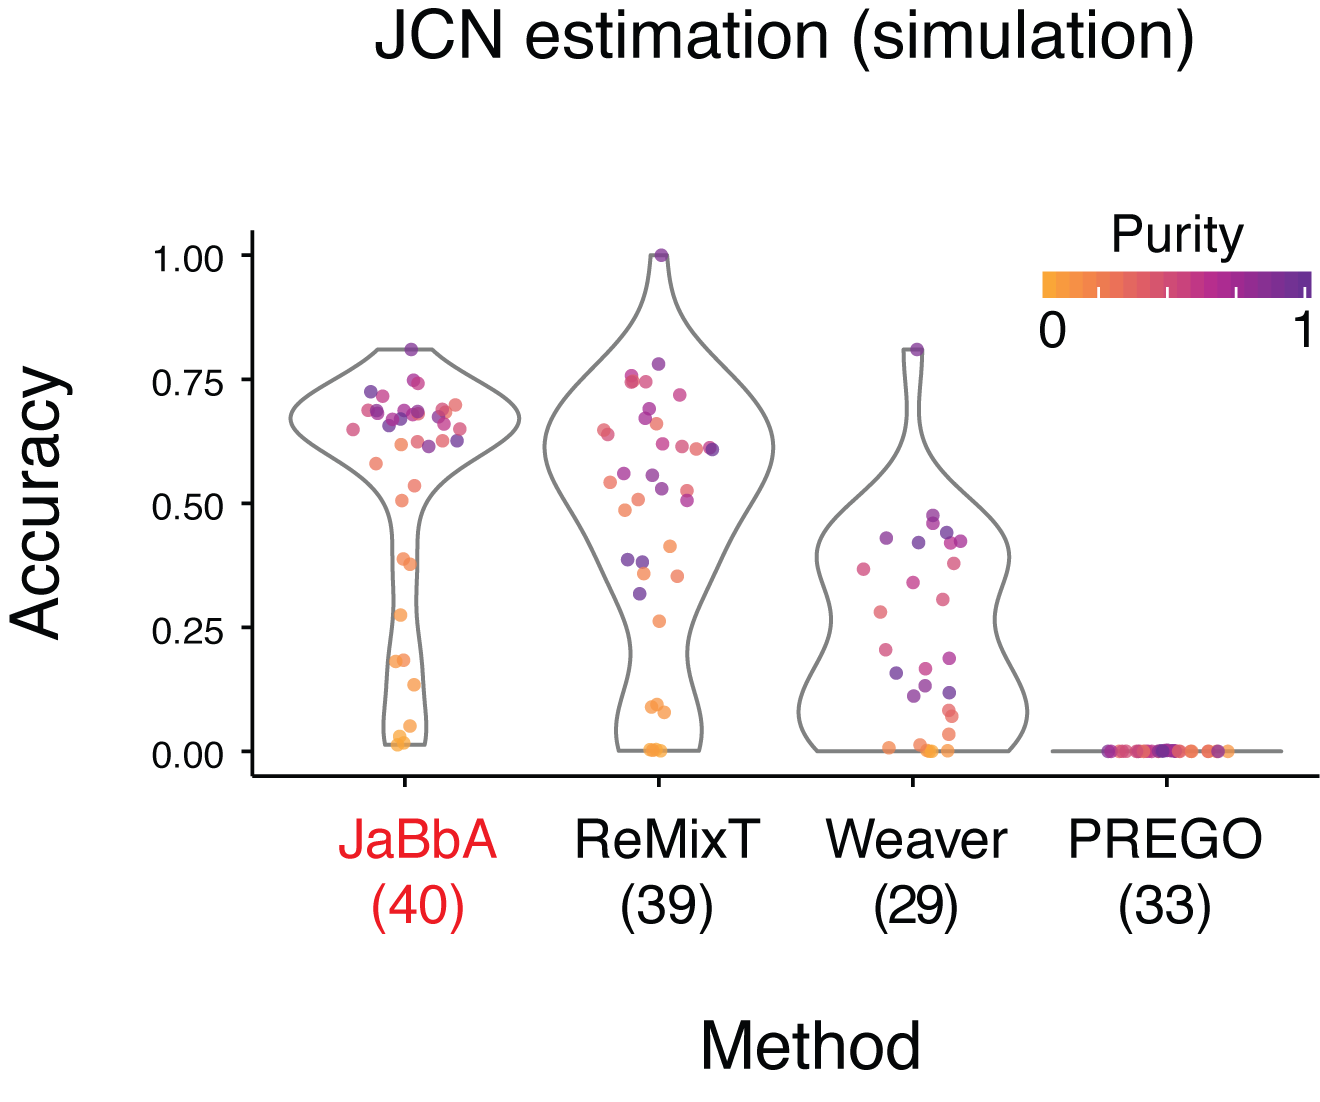
\includegraphics[width=0.95\linewidth]{figures/600ppi/jcn_accuracy_sim.png}
    \caption{\textbf{Junction copy number accuracy.}}
    \label{fig:jcn_accuracy_sim}
\end{figure}

\begin{figure}
    \centering
    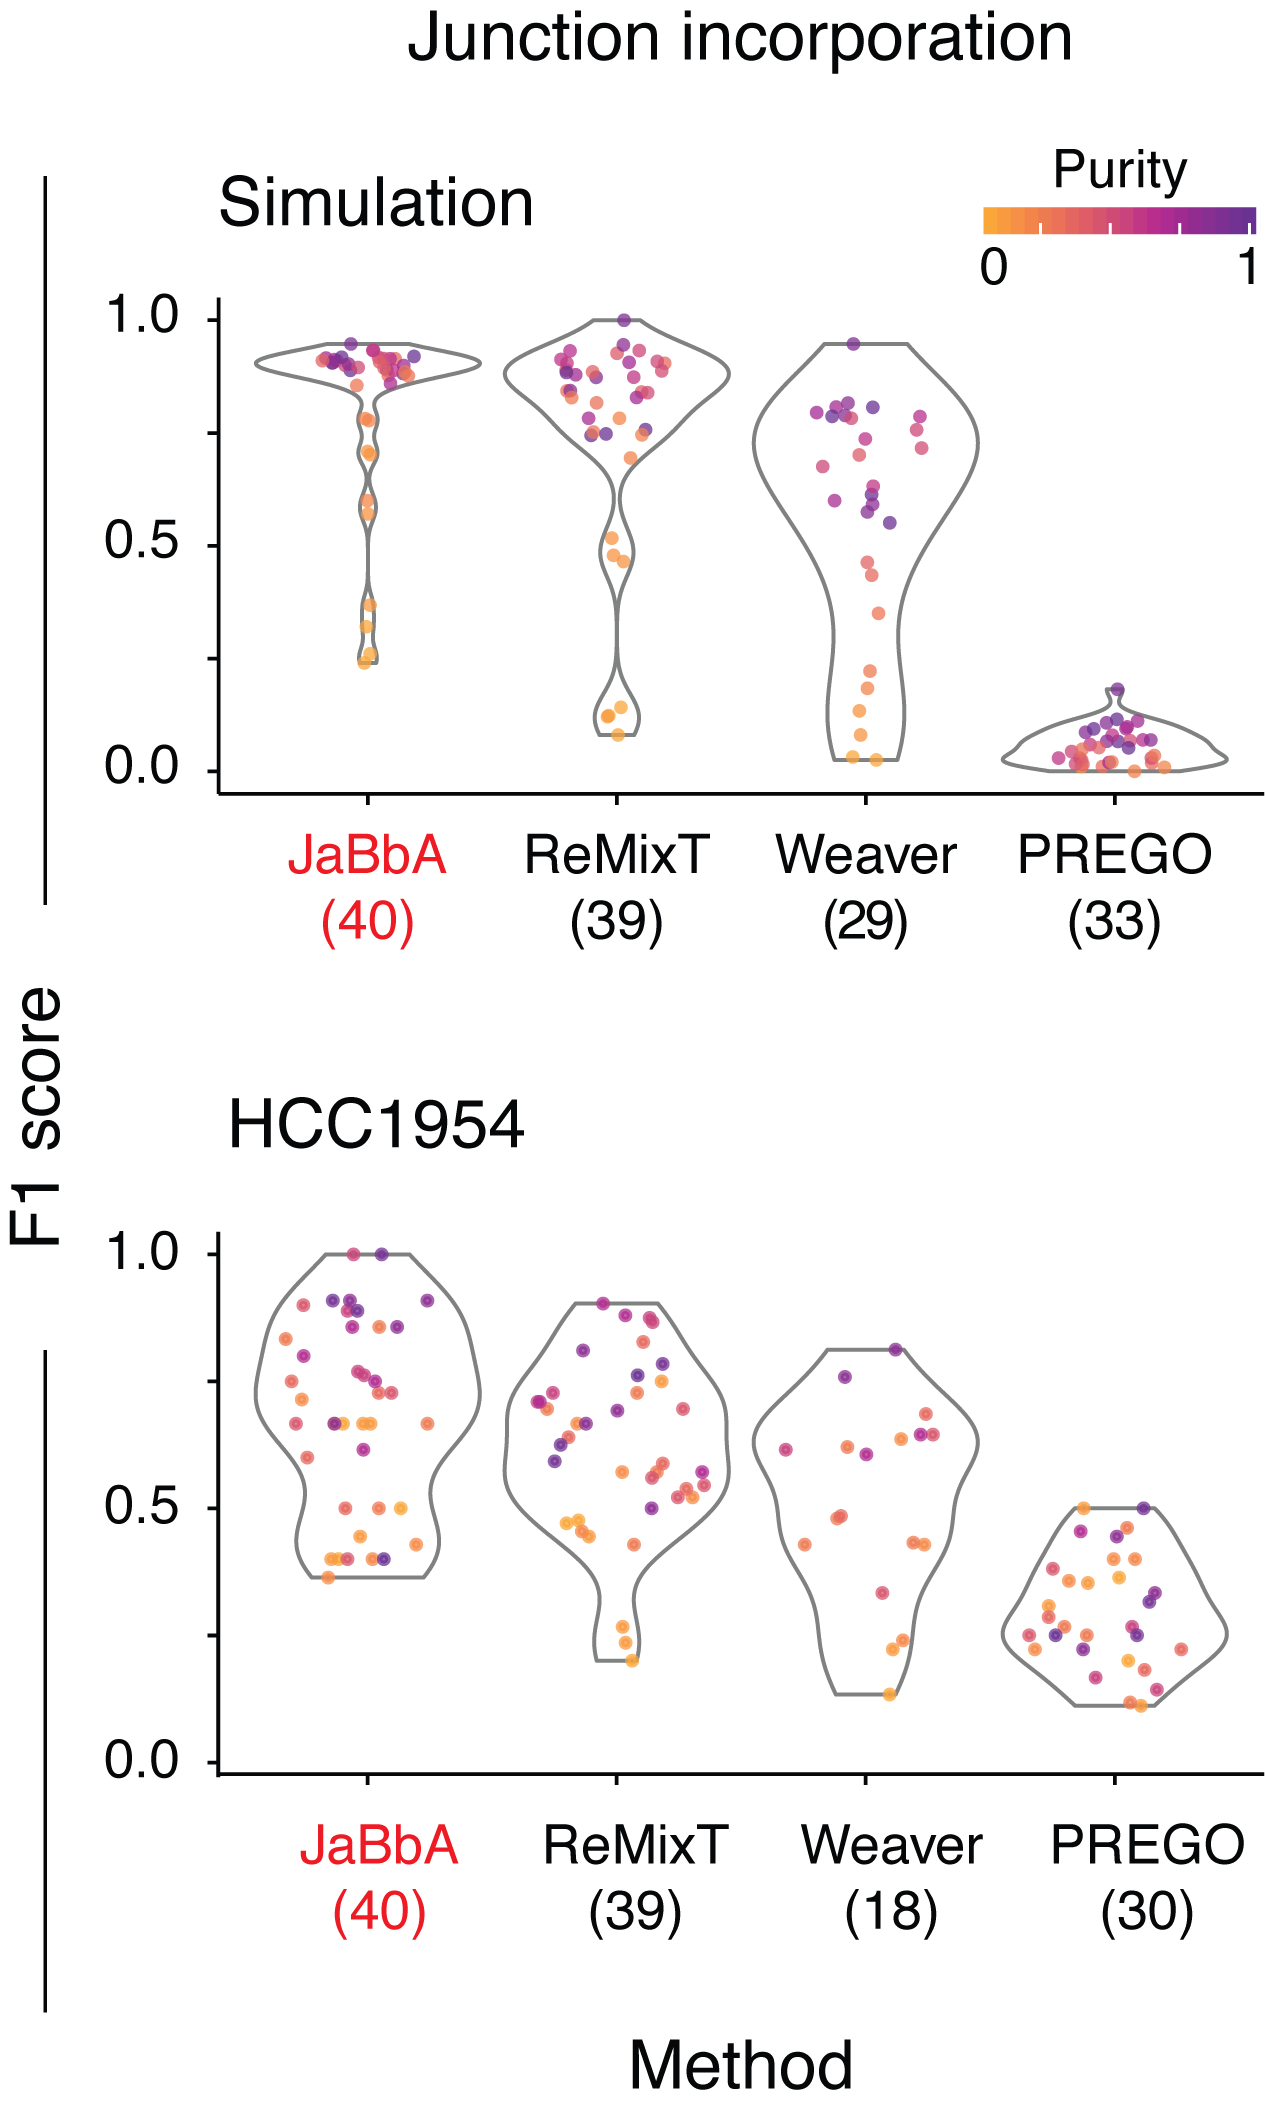
\includegraphics[width=0.95\linewidth]{figures/600ppi/junc_inc_f1.png}
    \caption{\textbf{F1 score of junction incorporation.}}
    \label{fig:junc_inc_f1}
\end{figure}

\begin{figure}
    \centering
    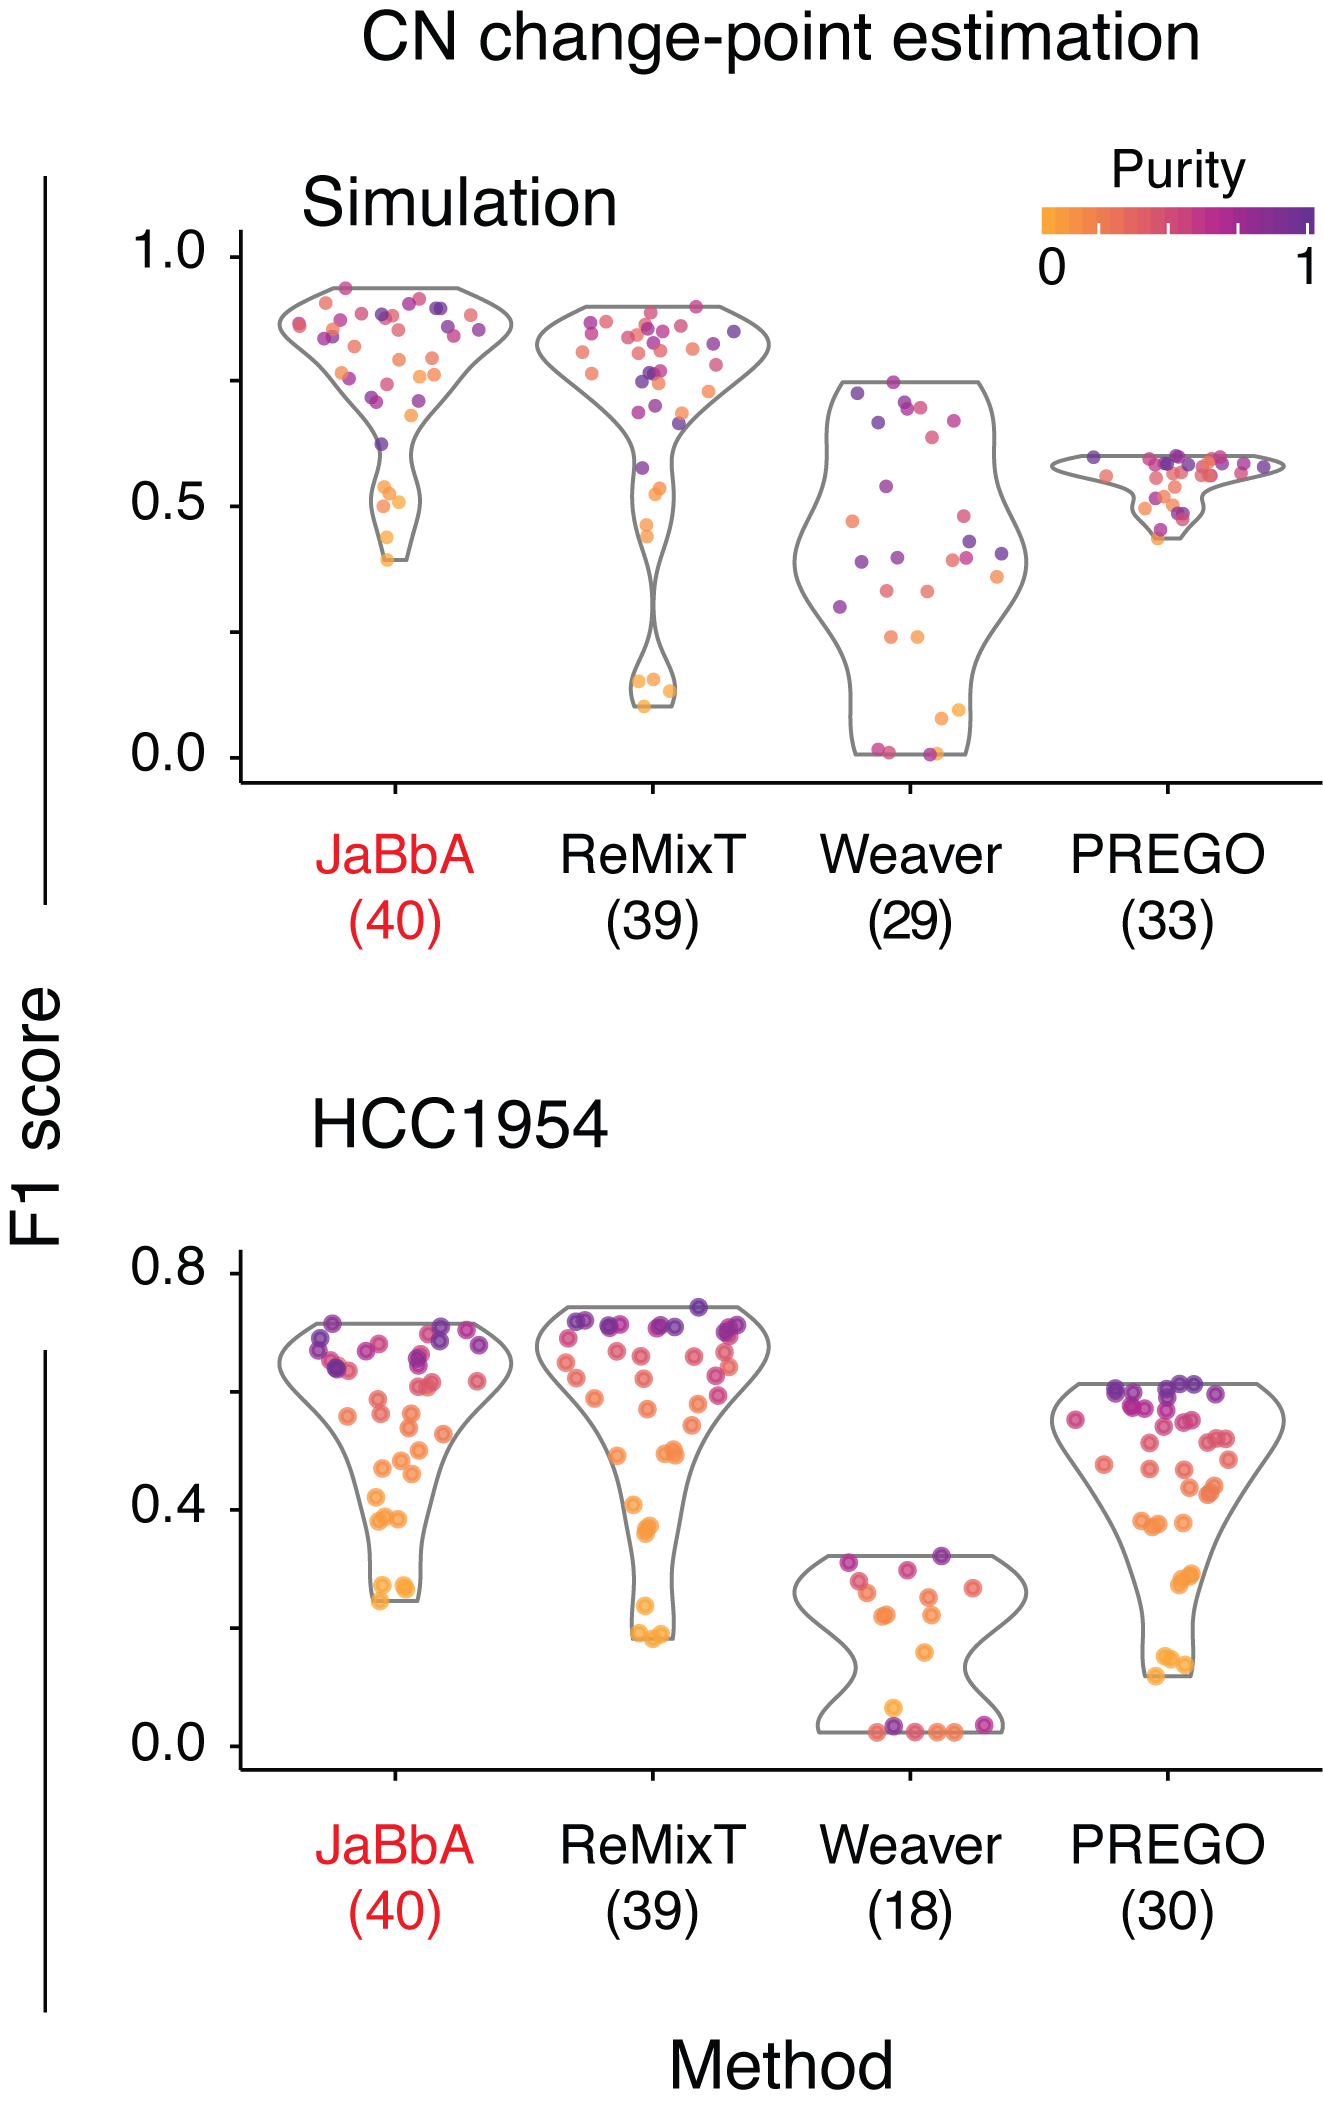
\includegraphics[width=0.95\linewidth]{figures/600ppi/cn_bp_f1.png}
    \caption{\textbf{F1 score of copy number change point placement.}}
    \label{fig:cn_bp_f1}
\end{figure}

\begin{figure}
    \centering
    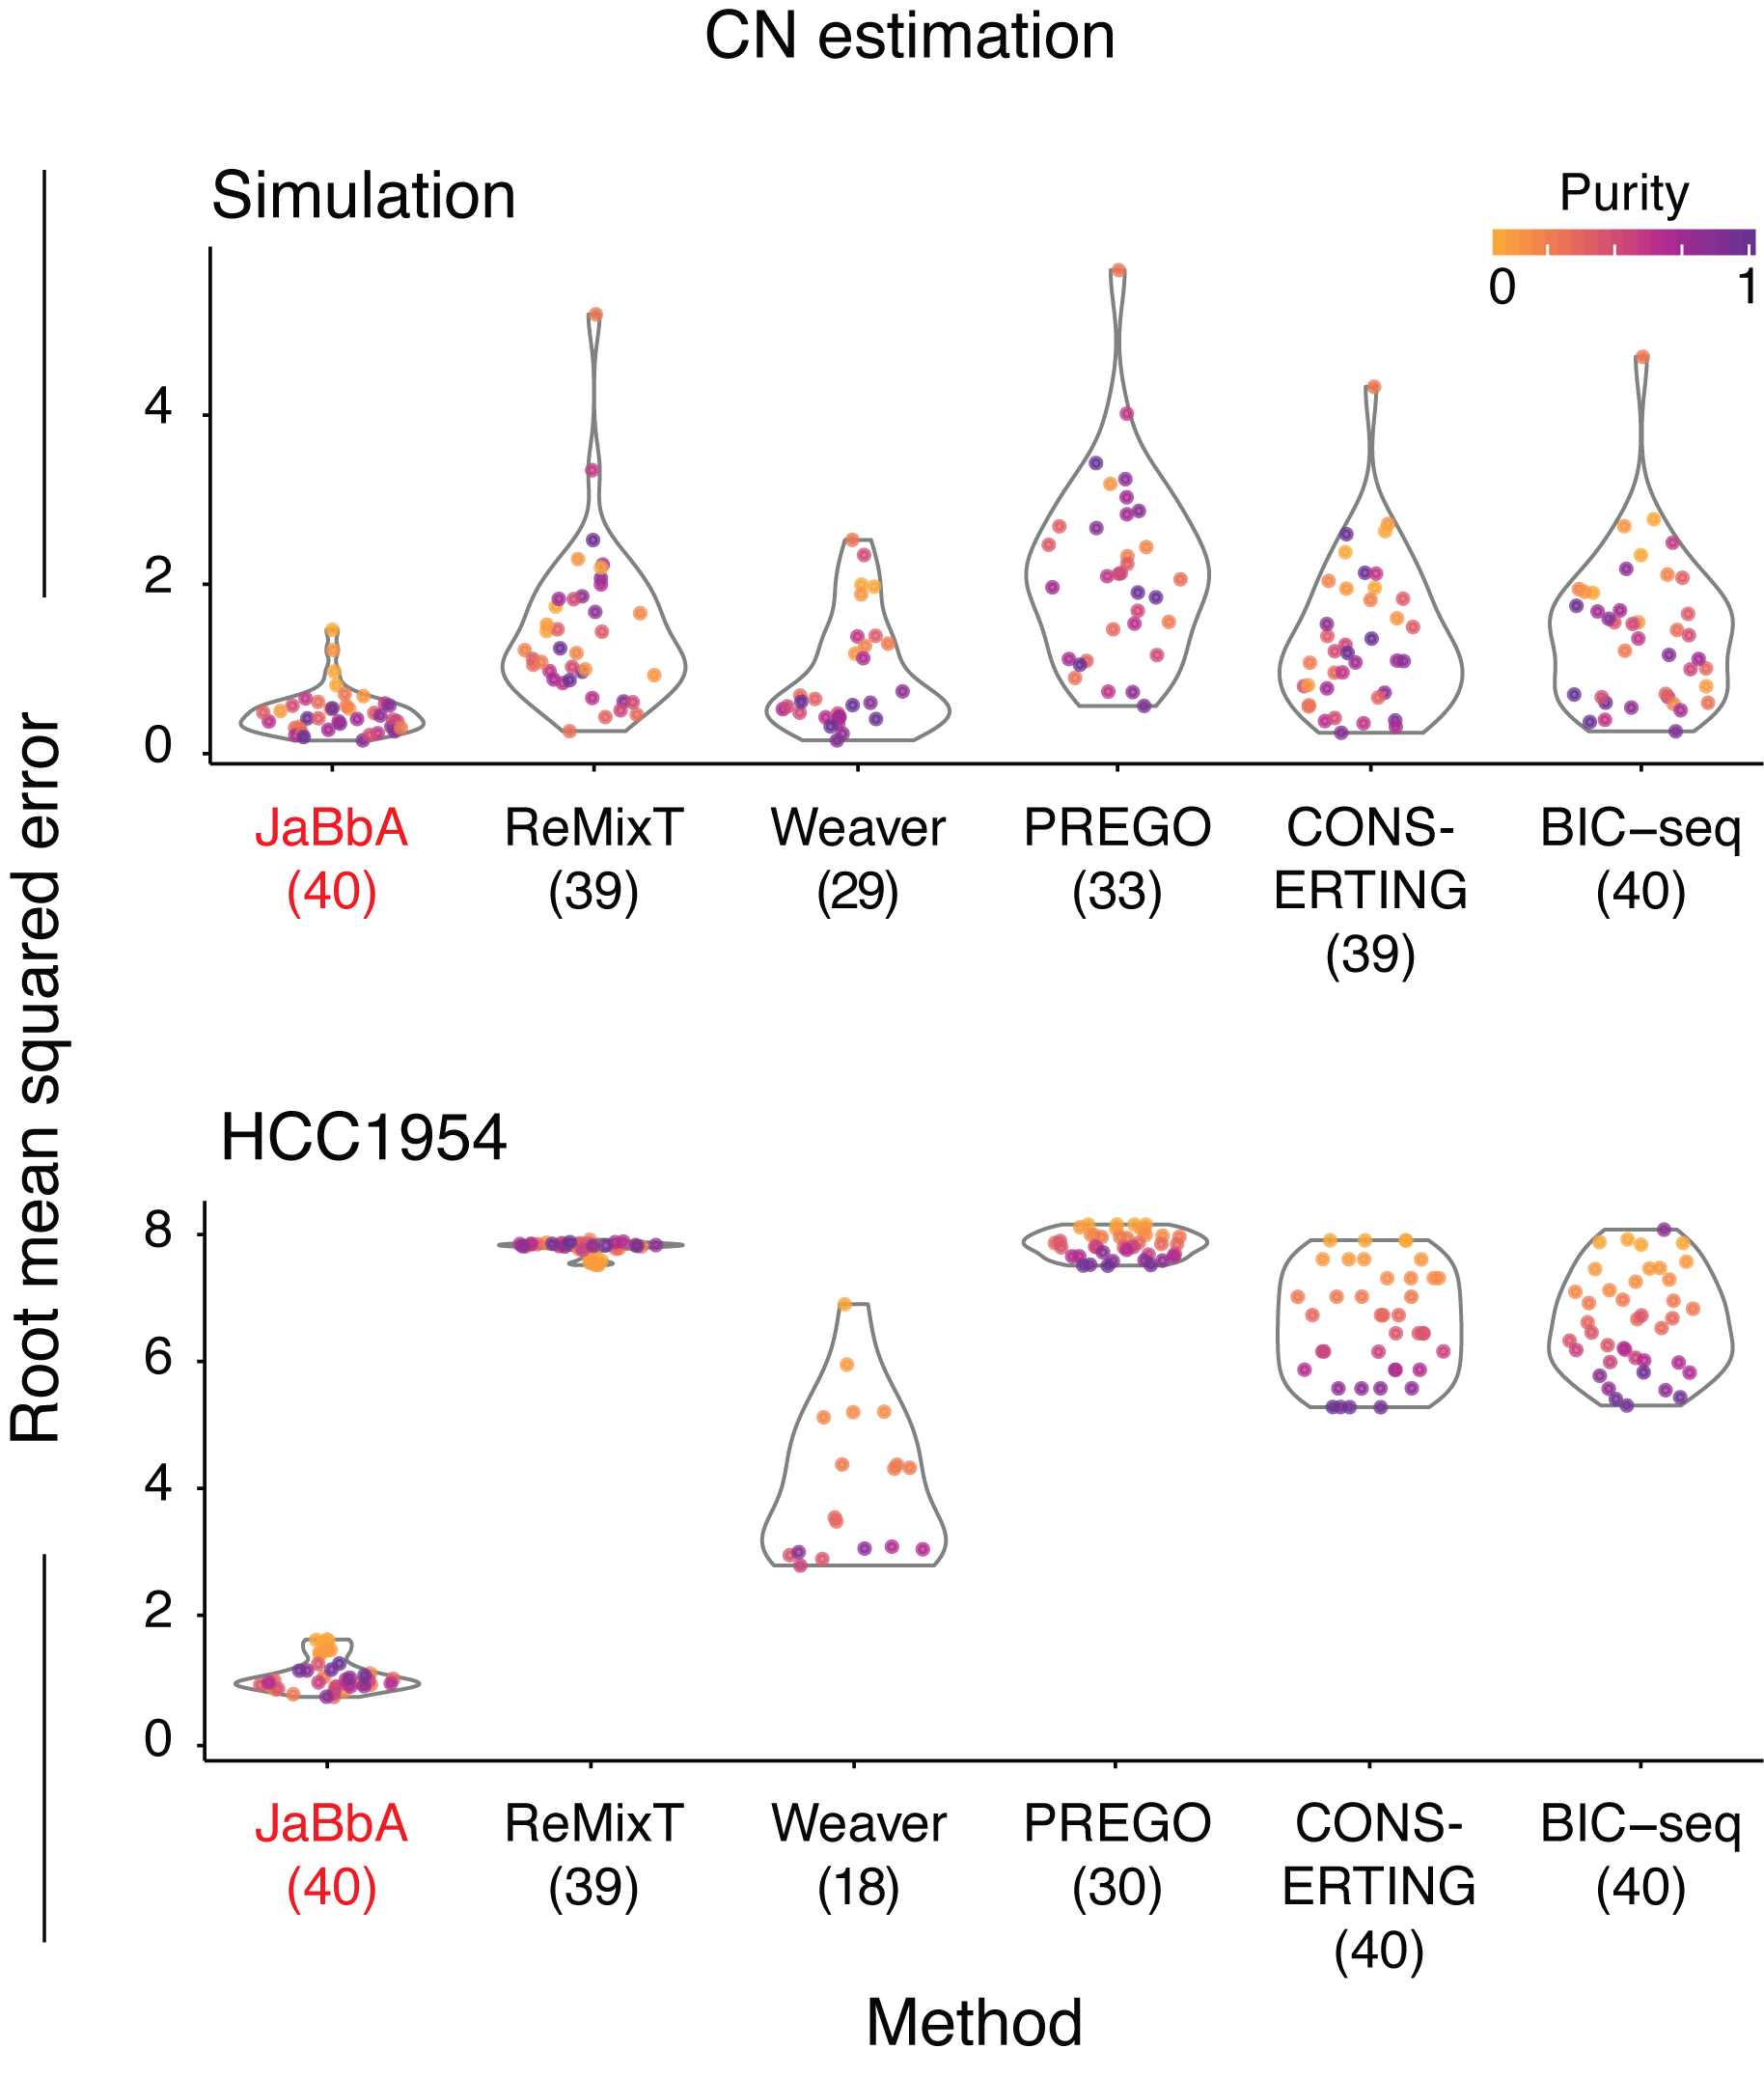
\includegraphics[width=0.95\linewidth]{figures/600ppi/cn_mse.png}
    \caption{\textbf{Mean square error of CN estimation.}}
    \label{fig:cn_mse}
\end{figure}

\begin{figure}
    \centering
    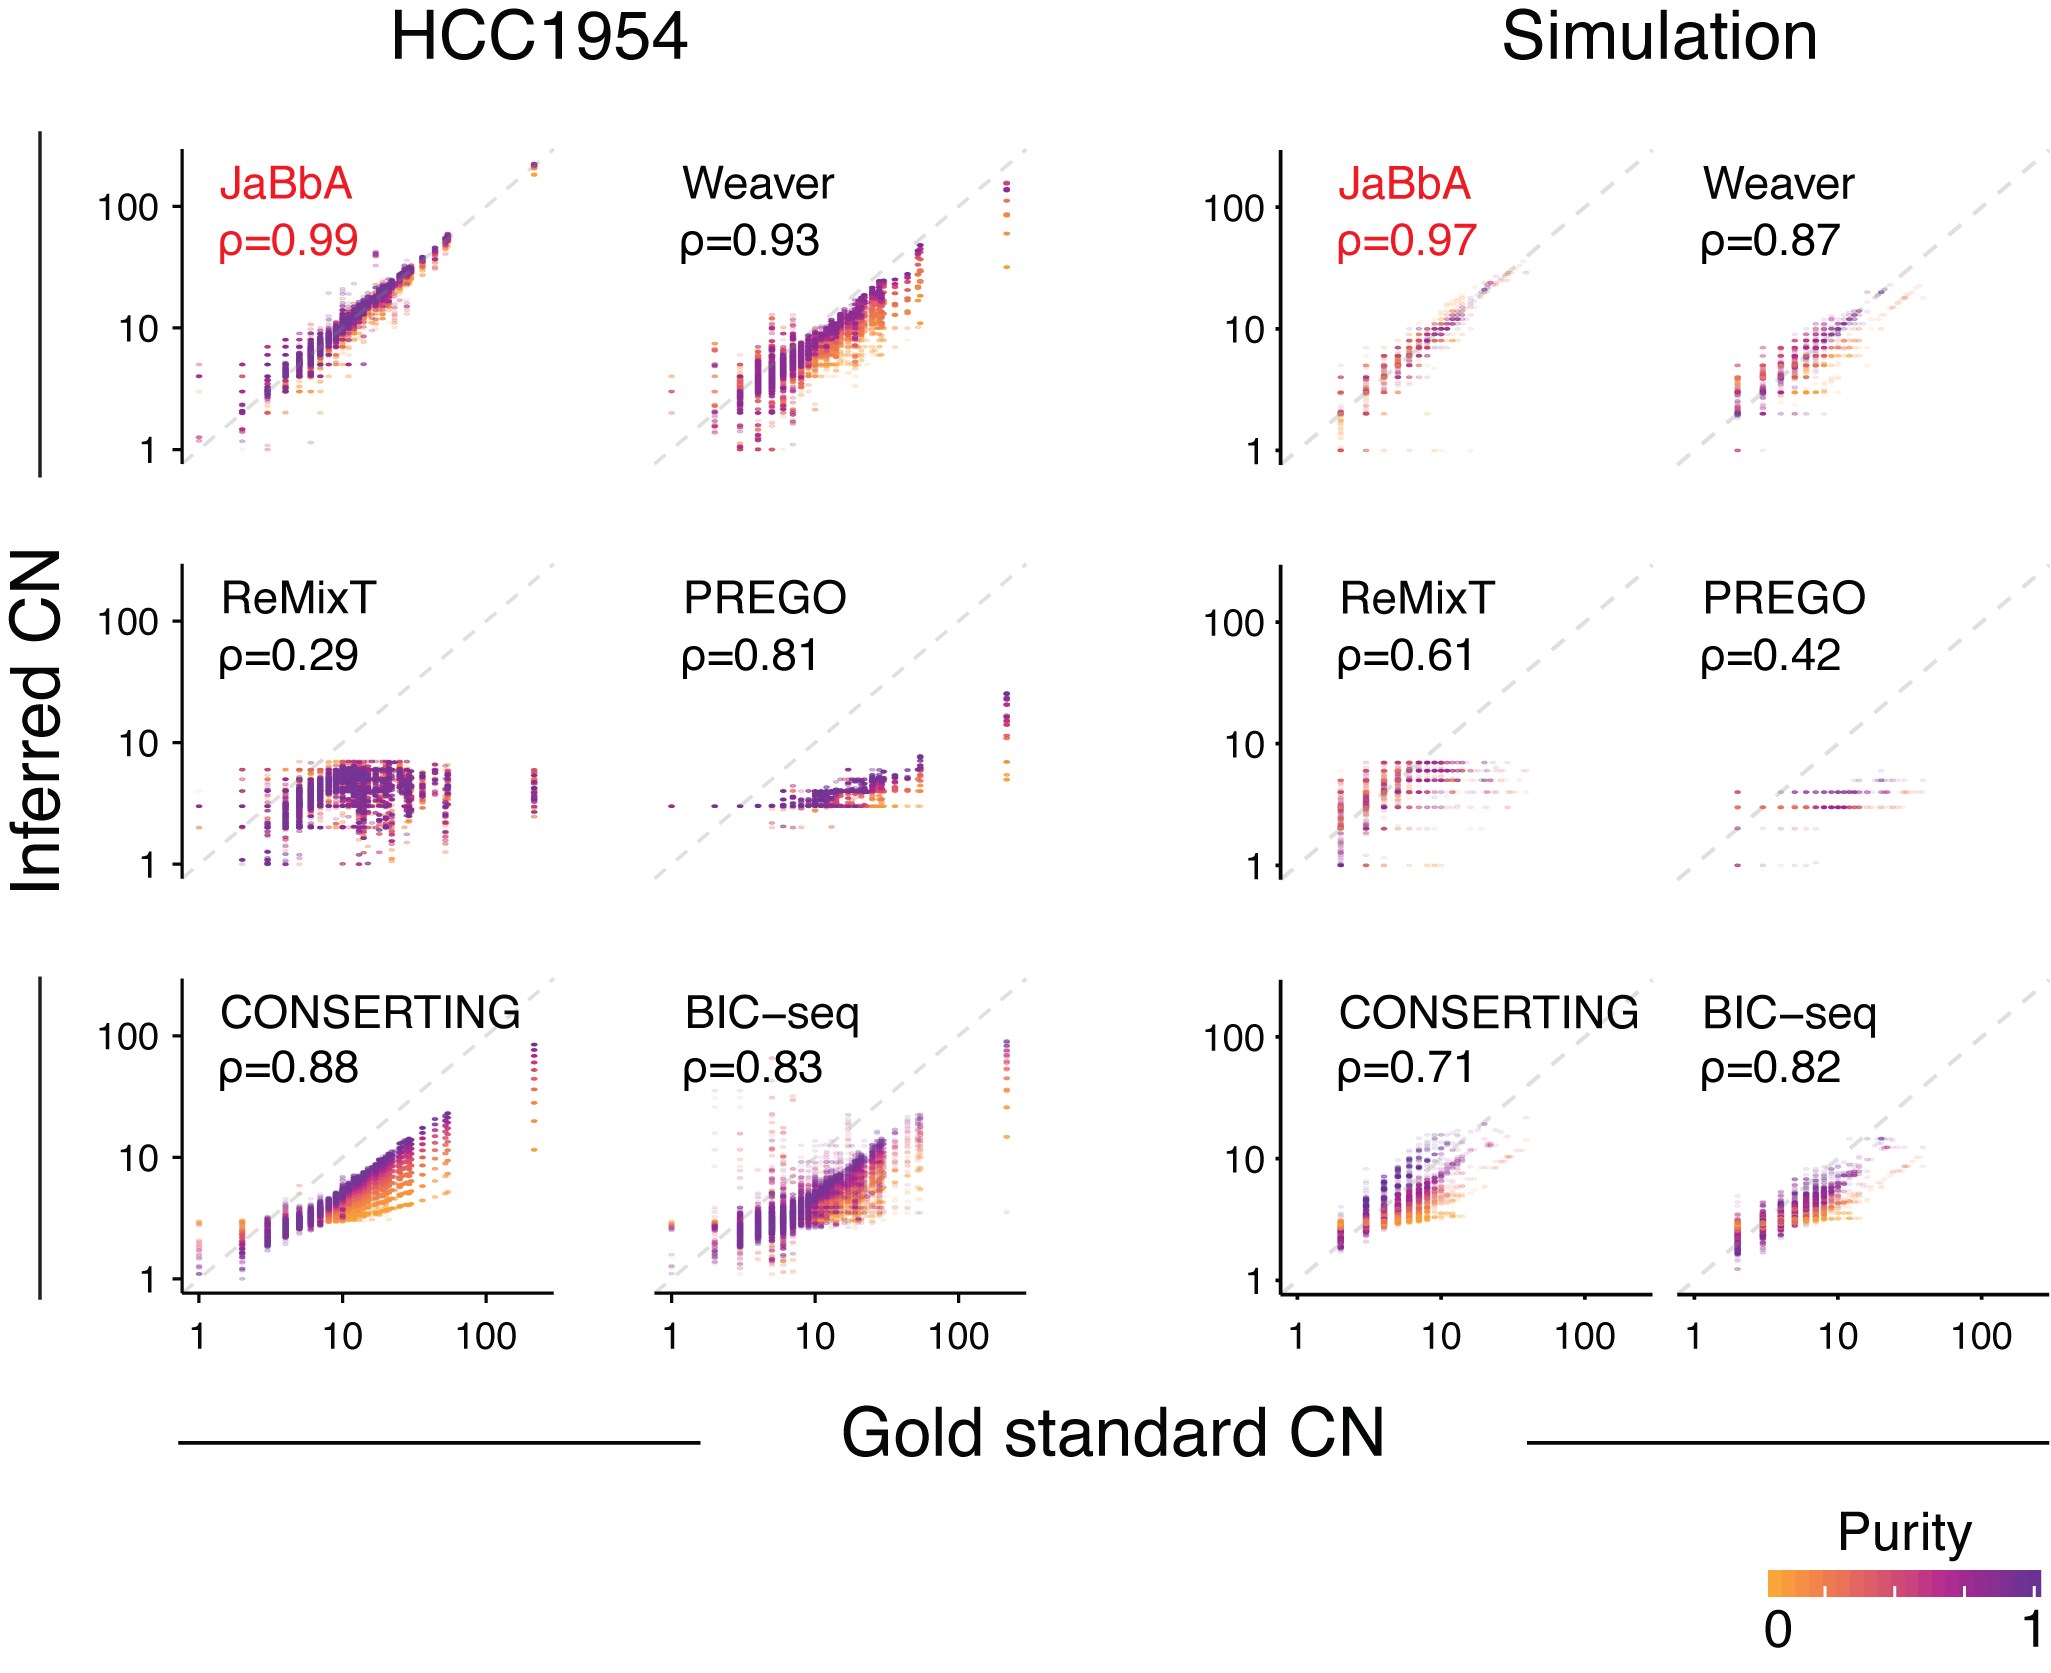
\includegraphics[width=0.95\linewidth]{figures/600ppi/cn_scatter.png}
    \caption{\textbf{Estimted versus gold standard CN.}}
    \label{fig:cn_scatter}
\end{figure}

\begin{figure}
    \centering
    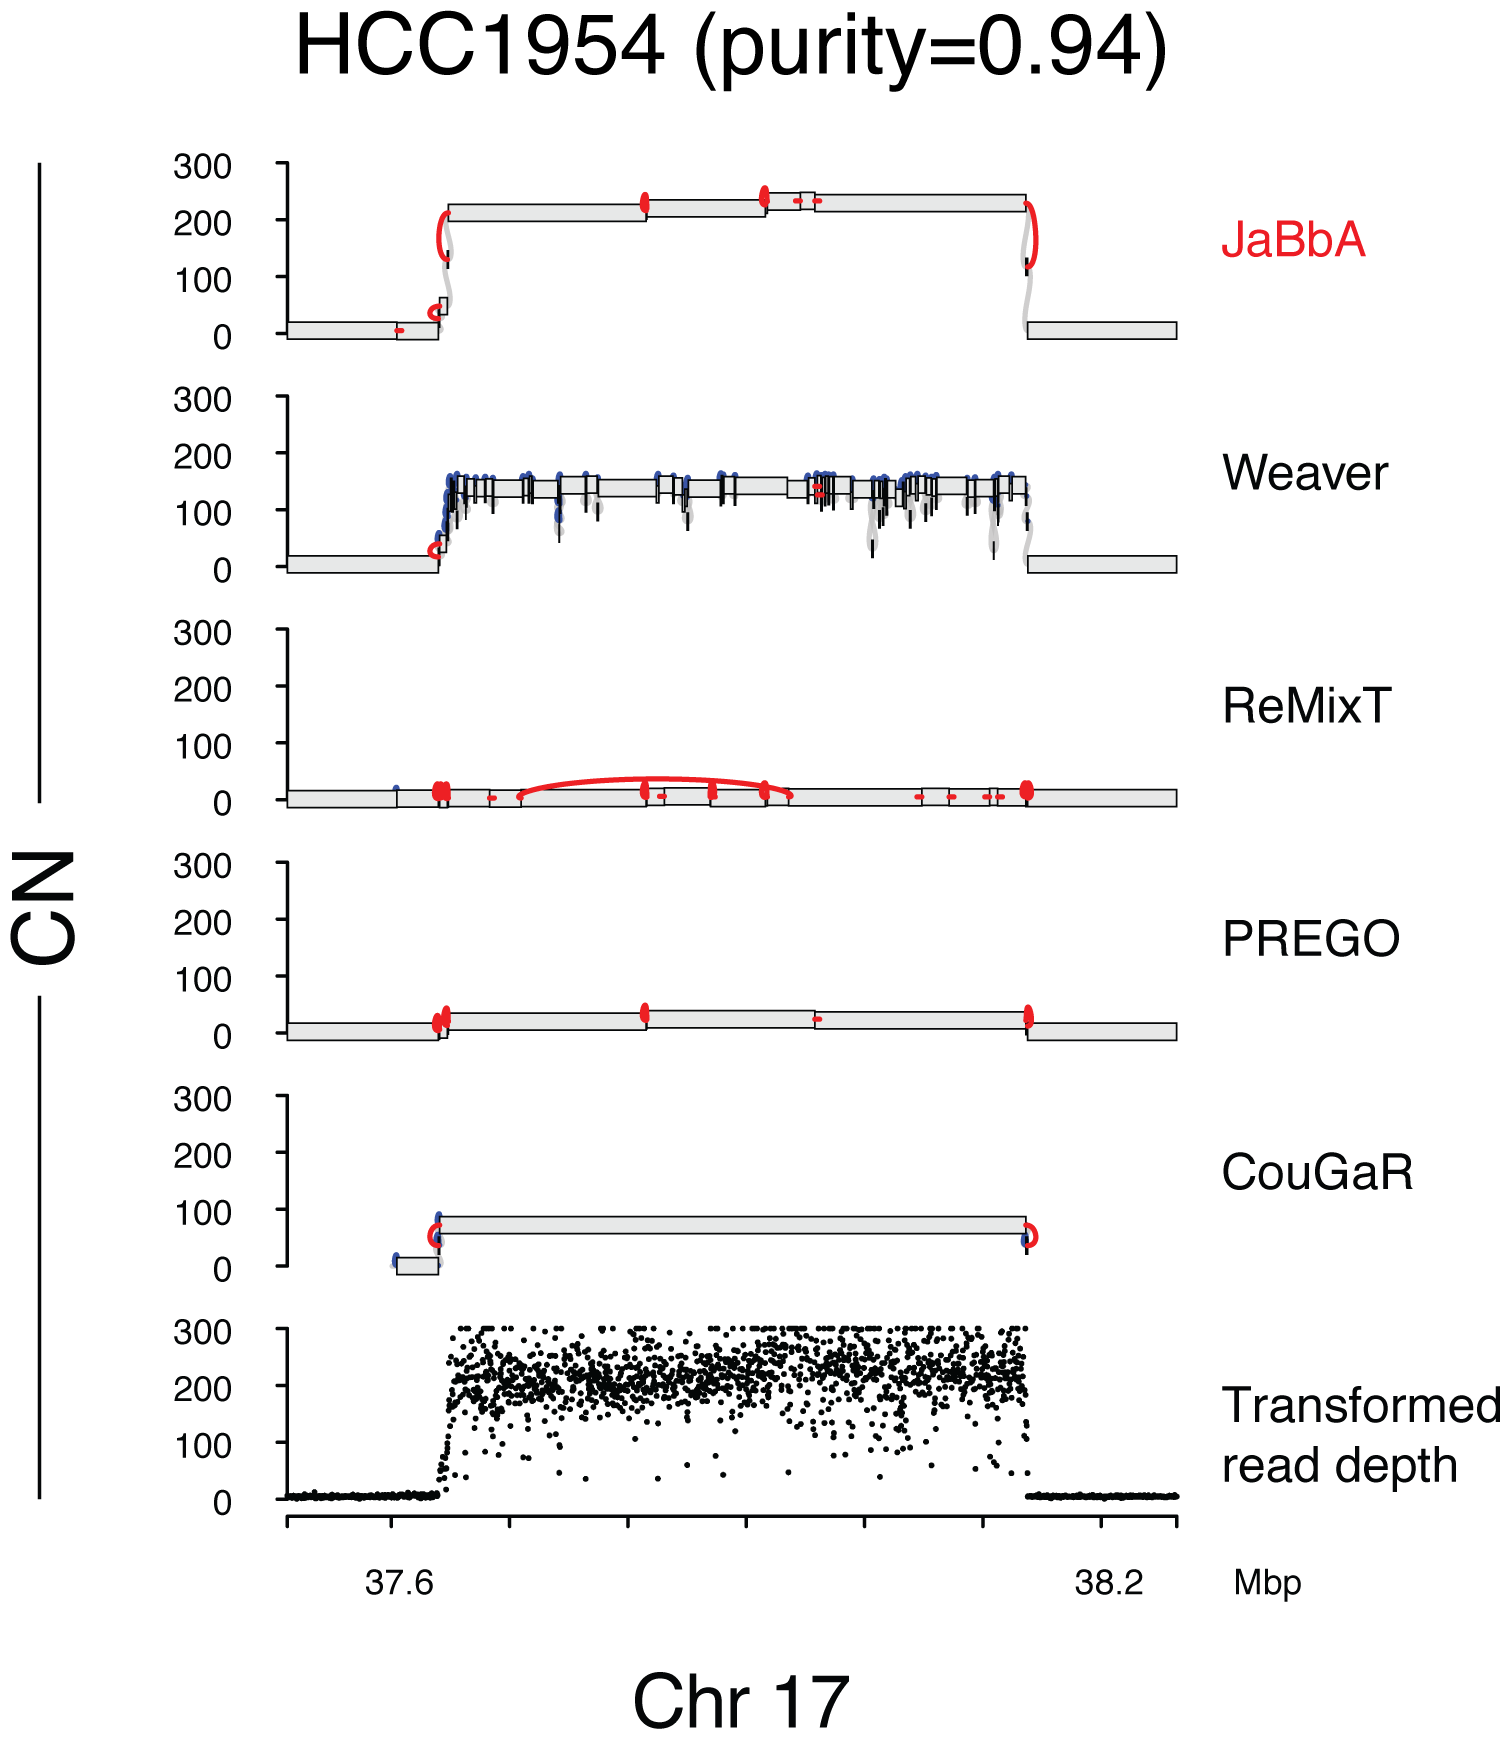
\includegraphics[width=0.95\linewidth]{figures/600ppi/example_bfb.png}
    \caption{\textbf{Reconstructed genome graph around HER2 amplification in HCC1954 cell line.}}
    \label{fig:example_bfb}
\end{figure}

The input junctions to all genome graph reconstruction methods were their respective default recommendations, namely SvABA unfiltered candidates for JaBbA; internal junction callers for Weaver, CouGaR; and the union of 3 junction calls (SvABA filtered \cite{wala2018}, Delly \cite{Rausch2012-ly}, Novobreak \cite{Chong2017-gl}) for PREGO, ReMixT, and CONSERTING as they make no default recommendations.  As a note, we saw very similar performance with JaBbA using standard settings (SvABA unfiltered junctions) and the union junction set (data not shown).

\subsubsection*{Junction incorporation and JCN estimation}
To evaluate junction incorporation and JCN estimation, the incorporated junctions were approximately matched to gold standard junctions, e.g. both breakends were within 1 kbp from the corresponding gold standard junctions with the same orientations. True positives were the number of matches, false positives were incorporated junctions without a match, and false negatives were gold standard junctions without a match. An F1 score of the incorporated junctions, the harmonic mean of precision and recall, was then computed for each benchmarking sample (\textbf{Fig. \ref{fig:S1}E}). Gold standard junctions for HCC1954 were defined as the consensus set inferred from the original high depth data (junctions identified by at least two callers out of SvABA, Delly, Novobreak).

Inferred JCNs of the graph reconstruction were compared to the matching gold standard junctions, if any, from the simulated dataset. The proportion of correctly fitted JCNs out of all incorporated junctions times recall of incorporation represented the accuracy or completeness of JCN estimation (\textbf{Fig. \ref{fig:S1}D}).

\subsubsection*{Segmental CN estimation}
When evaluating CNA inference performance, two metrics were considered. One was the correct placement of CN change points. Analogous to matching junction breakends, we considered an inferred CN change-point to match a gold standard if their distance was within 1 kbp and they have the same direction of CN change, e.g. increasing or decreasing CN from the side with smaller coordinates to the larger. To prevent spurious matching between inferred and gold standard CN change points, occurring in cases with excessive hypersegmentation, gold standard CN change points were only matched to the nearest identically oriented inferred CN change point.  Based on the matching, F1 scores were computed and shown in \textbf{Fig. \ref{fig:S1}F}. For HCC1954, the gold standard CN change-points were defined as the consensus junction breakends.

% Too many (hypersegmentation), too few (undersegmentation), too distant from the gold standard (large error margin) were all adverse indications. To prevent extreme cases of hypersegmentation being over-optimistic, each one of the gold standard CN change-points was only matched to the nearest correctly oriented inferred change point.

The other set of metrics reflects the concordance between the inferred CN profile with the gold standard. For each segment in the gold standard, the overlapping inferred segments were identified. The inferred CN for that gold standard segment was then defined as the overlap width-weighted average of inferred CN. Subsequently, the root mean squared error (RMSE) $\sqrt{\frac{\sum{(\hat{x} - x_{goldstandard})^2}}{n}}$ was computed across all gold standard segments for each sample (\textbf{Fig. \ref{fig:S1}G}). The gold standard for HCC1954 CN profile was derived from published microarray-based segmentation downloaded from the CCLE data portal. High-depth WGS coverage data was mapped onto these segments and transformed into copy number space using the known ploidy of 4.5 and purity of 0.99. To compactly show the relationship between inferred CN and gold standard from all runs, we drew scatter plots across all gold standard segments in all successful runs for each method, and the Pearson $\rho$ of each method was calculated from all data points pooled together (\textbf{Fig. \ref{fig:S1}H}).

%===========================%
\section{Implementation of genome graphs in gGnome package} \label{sec:implement_ggnome}
To facilitate the analyses of genome graphs, we built an R package \textit{gGnome} which allows fast and useful creation, exploration, visualization, and computation around genome graphs. The basic design principle is to keep the integrity of genome graphs, in particular the skew-symmetric property, on the backend with private fields and methods in R6 classes, while expose the most intuitive inputs and outputs like junctions and segments to the users.

% package structure
% construction
We constructed two main classes, \texttt{gGraph} and \texttt{gWalk}, corresponding to genome graph and walks. In the most basic form, a genome graph can be initiated with a reference genome alone, where each node is a chromosome and no edges exist (\texttt{gG()}). On top of that, we can segment the whole genome based on a set of breakpoint coordinates, by automatically connecting two consecutive nodes with a (pair of reverse complement) REF edge (\texttt{gG(breaks = breakpoints)}). When a ALT junction emerges, it joins two breakends that are not adjacent in reference genome to form new (pair of reverse complement) ALT edges (\texttt{gG(juncs = junctions)}). One can create any genome graph from the input data of segmentation (in a format equivalent to \texttt{GRanges}), and/or a set of junctions (in a format equivalent to \texttt{GRangesList}). More often in practical scenarios, we start from a copy number-annotated genome graph inferred from WGS. gGnome allows one to parse the results from most of the existing genome graph reconstruction methods (JaBbA, ReMixT, Weaver, PREGO, RCK, CouGaR, AmpliconArchitect).


% subgraph
With a genome graph (supposedly stored in variable \texttt{gg}), we can make a series of queries based on vertex and edge metadata, with the graph subsetting operator "[,]", where the expression before the comma filters the vertices and the latter filters the edges. For example, when looking up amplified subgraphs where the vertex CN is larger than twice the ploidy (supposedly stored in variable \texttt{pl}), one can execute \texttt{gg[cn>pl*2,]}. 

% viz by gTrack
To quickly explore any part of a genome graph, we integrated our static genome browser-style plotting package \texttt{gTrack}. With any genome graph, one can simply call \texttt{gg\$gtrack} to get the \texttt{gTrack} object to then plot using \texttt{plot} function. All the optional arguments of \texttt{gTrack} can be passed down natively from this interface. For example, if one wants to plot copy number stored in the metadata column "cn" on the Y-axis, it is as simple as \texttt{gg\$gtrack(y.field = "cn")}. As a more powerful alternative, we also provide interactive visualization through \textit{gGnome.js}, described in the next section. Here, with any \texttt{gGraph} object, one can simply generate the required JSON format with \texttt{gg\$json()}.

% distance
Given a genome graph, can also calculate a lower bound  shortest derivative (in the rearranged genome) genomic distance between any two genomic loci after rearrangements, by summing up the width of vertices the path traversed (encoded in the gGraph method \texttt{gg\$dist}). Taking advantage of the optimal implementation of Floyd-Warshall by the \textit{igraph} R interface, this can be immediately scaled up to find all shortest paths from one set of genomic loci another set, encoded in the function \texttt{proximity}.

% clusters
One of the more interesting topics in SV pattern discovery is the clustered junctions. We can easily cluster vertices and/or edges based on their connectivity, implemented in \texttt{gg\$ecluster} for edges and \texttt{gg\$cluster} for vertices. The output cluster membership (weakly connected or strongly connected), will be recorded in a metadata column and can be used to retrieve the corresponding subgraph, for instance, \texttt{gg\$ecluster(); gg[,ecluster==1]}.

% maxflow
Besides, with a non-negative numeric field associated with vertices and edges, for example, copy numbers, we can also regard that as \textit{capacity} in traditional flow problems. For example, the \textit{max flow} problem with CN means the "maximum number of copies of such DNA molecules that connects genomic locus A and B".

% event calling
Next, we provide functions to replicate our algorithms in \cite{Hadi2020-um} and this disseration for finding the subgraphs of 13 different SV events. The \texttt{events(gg)} function will automatically search the given graph for these patterns with the default parameters and annotate any findings in the metadata columns with the name of the event, like "chromothripsis". Plus, after running the function, there will be a new data table of all the findings appended to the field of \texttt{gg\$meta\$events}.

%===========================%
\section{Neo-connectivities on a genome graph encode putative functional events}
As explained in the previous sections, a walk (and its reverse complement walk) on a genome graph maps to a linear DNA sequence. If there exists a possible walk between two vertices it means the genomic elements within the two vertices may be connected on a contiguous DNA segment in the sample, if and only if all the ALT edges along the walk are phased in cis. A pair of ALT edges phased in cis means there are at least one copy of them found on the same DNA molecule; while none such copy is found they are deemed phased in trans. In reality, due to the large size of the genome and the limited read-length or effective range (e.g. for linked reads), complete phasing of all junctions is near impossible for most cases. However, the connectivities between genomic regions on the un-phased or partially phased genome graphs can serve as an approximation.

As we established in earlier sections, a complete genome graph should enclose all the walks corresponding to the studied genome, so if any copy of two genomic loci are on the same part of a DNA molecule, that segment should have a corresponding walk on the complete genome graph. Based on this observation, the new genomic distance after rearrangements between any copy of two loci is summing over the width of vertices plus the within-vertex distances to the incident ends along the walk for the starting and terminating vertices. Thus, even when it is not possible to exactly decompress the graph to the walks consistent with the actual karyotypes, we know that the real shortest genomic distance between any copy of two loci should not be shorter than the shortest path distance on the complete genome graph.

Admittedly, there may never be a complete genome graph constructed with the current technologies, and it is always possible that we failed to identify certain junction like centromeric \cite{Cameron2021-db} or involving repetitive or foreign sequences \cite{Behr2021-gf} and those may cut some genomic distances even shorter. Nevertheless, as shown in \cite{Behr2021-gf}, the state of the art short-read WGS should be effective at catching the majority of somatic rearrangements. Plus, even with the imperfect genome graphs, we can already expand the repertoire of functional genomic events by including the complex events. We use this approximation to show that potential functional events of arbitrary complexity can be represented as walks on genome graphs, exemplified by bridged fusion genes and enhancer hijacking.

Some fusion genes have long been established as cancer drivers and even successful drug targets \cite{Gao2018-nm}; some have also been shown to encode chimeric proteins that can trigger immune responses as neoantigens \cite{Rathe2019-cr}. Expectedly, most fusion genes found to date are created by one somatic junction, as it requires fewer junctions to create and has simpler topology to detect. However, in theory, there should be no biological restraint against a more complex, multi-junction fusion gene. Indeed, recent large pan-cancer whole genome and transcriptome profiling efforts have identified numerous such examples termed \textit{bridged fusions} \cite{PCAWG_Transcriptome_Core_Group2020-zp,Yun2020-bi}. Naturally following our above definition, any fusion genes, no matter how many somatic junctions is involved, can be represented as a walk $w = (v_1, e_1, v_2, ..., e_{k-1}, v_k)$ on the corresponding genome graph, where the 5’ partner is at the outgoing end of $v_1$ and the 3’ partner is at the receiving end of $v_k$ (Fig x). Here I show an example walk of xxx—xxx fusion found by the PCAWG Transcriptome working group \cite{PCAWG_Transcriptome_Core_Group2020-zp} along with the supporting reads from the RNA-seq. By our graph-based SV event classification, this junction was part of a large scale xx (described in the next chapter).

% TODO!!! FIGURES
Another class of emerging SV driver events are enhancer hijacking, where an active yet distal enhancer is juxtaposed near a dormant proto-oncogene, activating its expression. In thyroid carcinoma, the insulin-like growth factor 2 mRNA-binding protein 3 (IGF2BP3, chromosome 7p15.3) has been found to be activated and contribute to cell proliferation by being juxtaposed next to thyroid adenocarcinoma-associated (THADA, chromosome 2p21) gene \cite{Panebianco2017-xt} which is constitutively expressed in normal thyroid tissue. This event is later confirmed by PCAWG consortium \cite{Rheinbay2020-no} to be recurrent in at least 5 different thyroid carcinomas it profiled with WGS. I reconstructed all these 5 paths that consist of only one junction each (FIGURE!!!!)

%===========================%
\section{Interactive visualization of genome graphs in arbitrary genomic windows}
% from JaBbA 
To visualize the genome graphs we developed \texttt{gGnome.js} (source code at \url{https://github.com/mskilab/gGnome.js}), a Javascript-based genome browser that renders genome graphs and allows for interactive browsing across discontiguous genomic intervals accompanied by various genomic annotations. Here, we describe several important and unique features of gGnome.js.

% gGnome.js figure
\begin{figure}[h!]
    \centering
    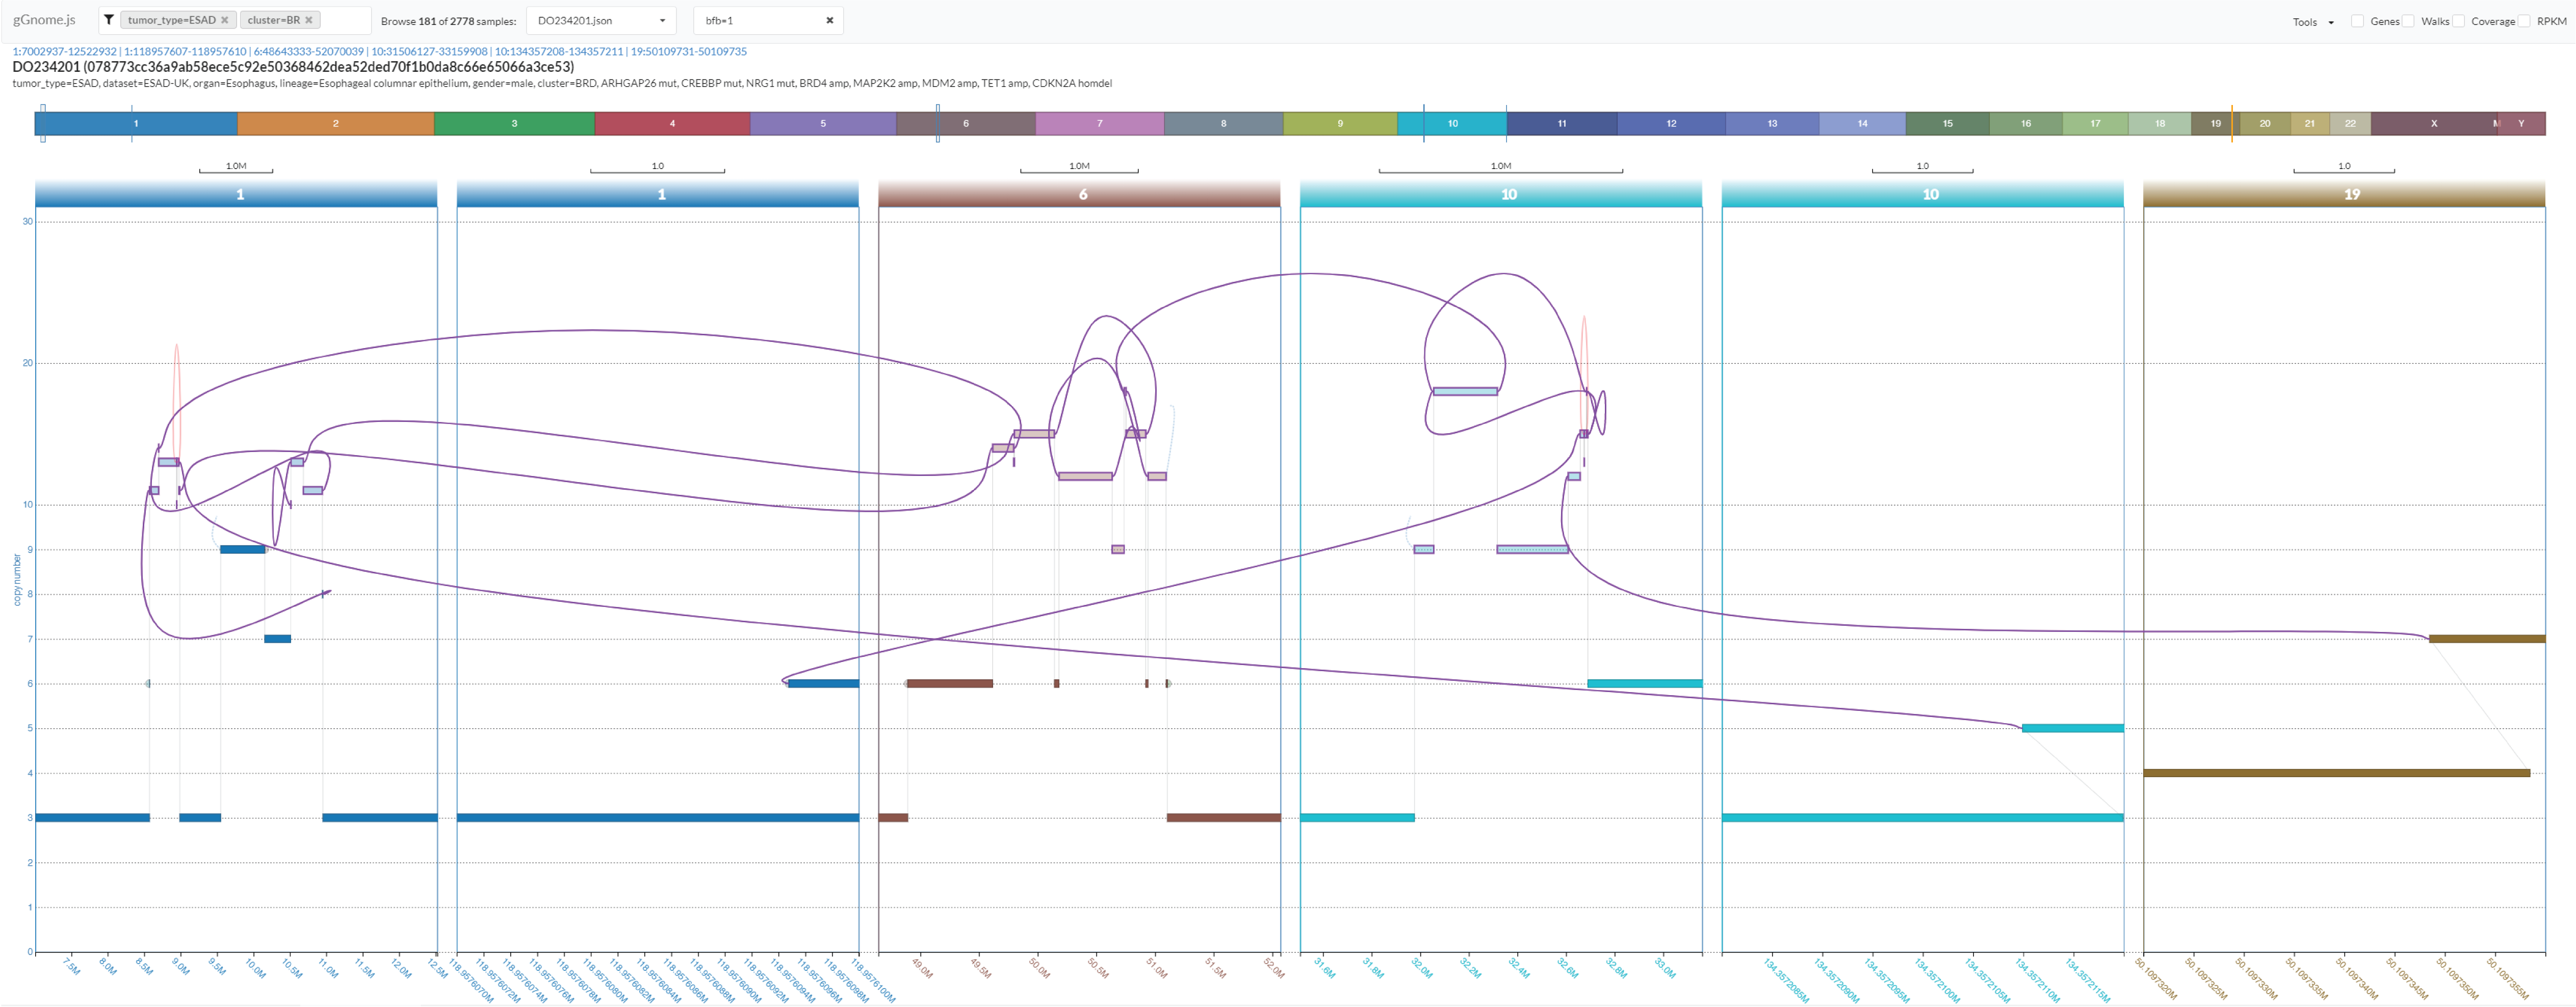
\includegraphics[width=0.95\linewidth]{figures/600ppi/ggjs.png}
    \caption{\textbf{A snapshot of the gGnome.js interface of a BFBC event in an esophageal adenocarcinoma sample.}}{}
    \label{fig:ggjs}
\end{figure}
% 
First and foremost, the flexibility of arbitrary window browsing is crucial for complex rearrangement events, which can vary in scale and involve many distal loci. Annotations of events (or any set of vertices/edges) were read by the browser and can be searched. For example, in Figure \ref{fig:ggjs} we can visualize a multi-chromosomal breakage-fusion-bridge cycle (BFBC) event in 6 discontiguous windows spanning 4 different chromosomes and locate this event instantly with the \texttt{annotation} selector on the top right corner.


Annotations corresponding to segment-level and also junction-level information were included in the browser. Metadata for segments includes, but is not limited to, total copy number, allele-specific copy number (for samples and intervals in which heterozygous SNP information is available, i.e. cases with both tumor and normal pairs), and correspondence to event type if the segment was identified as part of an event. Edge metadata includes information output by the SV caller used in this study, SvABA, including number of reads supporting the SV and junction topology. These metadata can all be presented when the cursor hover over a specific element.

Second, the \texttt{gGnome.js} browser enables visualizing any genome graph, either with CN as inferred by other graph callers, or even without CN in the case of plain genome graphs. 

As a meaningful default, we plot integer copy numbers of the segments on the Y axis, that are inferred from cancer whole genome sequencing (WGS) with JaBbA (described in the next section), making it ideal for quick browsing copy number aberrations and immediately reveal the architecture of the complex events. 

%Annotations on subgraphs are searchable and useful to mark interesting events (like chromothripsis). A sample level search engine accelerates the browsing on large cohorts. We can also plot possible karyotypes as walks within the graph assisting on the identification of functional neo-connectivities or clarification of complex event topologies.

Third, when visualizing a larger cohort an integrated tag filter helps narrow down desired samples by any metadata string, exemplified by primary cancer types, data source projects, mutation status of genes.

Fourth, gGnome.js also supports visualizing additional genome tracks in the format of scatter plot, bar plot, and gene annotations, whose visibility can be controlled by the functionnalities in the top right corner.

% newly written
%To bring genome graphs better intuition for practical use, we developed \textit{gGnome.js} (https://github.com/mskilab/gGnome.js), a web application that draws genome rearrangement graphs onto its reference coordinates and allows for interactive browsing in any number of discontinuous windows accompanied by various types of genomic annotations. By allowing arbitrary windows and navigation by connectivities, the users can traverse the genome freely and simultaneously inspect various data at multiple relevant locations, including numeric (like read coverage) and qualitative (like gene annotations).

%===========================%
\section{Discussion}
In this chapter, I defined a skew-symmetric direct graph representation of a rearranged genome, termed genome graph. Genome graphs are general enough to encapsulate all junctions which have corresponding coordinates within the reference genome, and thus can represent SV events of arbitrary complexity that create many junctions. Compared to variation graphs \cite{Hickey2020-cu} such formulation is almost equally general, except for foreign sequences and variants that cannot be associated with a coordinate (e.g. small non-templated insertions), yet exceedingly light-weight as the vertices are free of the burden to carry the actual sequences. Although here I only described the usage of genome graphs in representing cancer genomes with SVs, it is straightforward to use for germline SVs and concatenate to form population pangenome graphs too \cite{Siren2020-tf,Eizenga2020-cf}.

Specifically for cancer genomics, genome graphs are an ideal data structure to bridge the fragmented yet high-throughput short-read sequencing, and the emerging long-range, long-read sequencing or optical mapping techniques. Junction-balanced genome graphs (JBGGs) are stoichiometrically plausible compressions of all possible derivative sequences that can result from the junctions they contain, and can be used to generate a pool of walks which provide substrates for finding an optimal linear combination of alleles like that maximizes parsimony or likelihood of generating an observed long-range pattern \cite{Hadi2020-um}. 

Even without the exact inference of linear alleles, we can still find useful bounds from the pool of all possible walks for many applications, because when the genome graph is complete, the true walk must be contained within. So we can approximate the genomic distance between two reference coordinates in the face of SVs using the shortest paths distance on the genome graph. Using  in thyroid carcinoma \cite{Panebianco2017-xt} as an example, I recaptured the 5 THCA samples with the THADA-IGF2BP3 enhancer hijacking event reported by PCAWG \cite{Rheinbay2020-no}, and further discovered a case where the juxtaposition of THADA near IGF2BP3 is achieved by two junctions from a more complex event, which also elevated the expression of IGF2BP3 like in the cases found in.  A special example is that fusion genes can be regarded as two genes (or transcripts mapped back to DNA coordinates) joined by junctions and whose inter-gene distance becomes zero along a path in the genome graph. 

Furthermore, thanks to programs like JaBbA \cite{Hadi2020-um}, InfoGenomeR \cite{Lee2021-rl}, the problem of inferring a JBGG from a short-read whole genome sequencing is a generically tractable and robust to most sample purities. JaBbA differs primarily from previous genome graph methods in its robust modeling of WGS read depth noise and explicit accounting of false negative junctions, also called loose ends (see \nameref{sec:methods}). In our benchmarking experiments, JaBbA inferred JCN with consistently higher fidelity than published genome graph-based methods (ReMixT \cite{McPherson2017-ry}, Weaver \cite{Li2016-qa}, PREGO \cite{Oesper2012-vw}) across a wide range of tumor purities (\textbf{Fig. \ref{fig:S1}D-E}). Particularly, concerning the HCC1954 experiment, JaBbA is the only caller that has a wide enough dynamic range to accurately capture the extremely high CN of the ERBB2 complex amplicon (Figures \ref{fig:bfb_example},\ref{fig:cn_scatter}) while correctly placing the junctions. This is the benefit of using a linear programming formulation with properly penalized loose ends.

In addition, JaBbA qualitatively outperformed genome graph-based methods and even classic (i.e. non-graph based) CNA callers (BIC-seq \cite{Xi2011-oa} and CONSERTING \cite{Chen2015-sw}) in estimating interval CN and change point locations across a wide range of tumor purities (\textbf{Fig. \ref{fig:S1}F-I}) as it utilizes the extra precision from the junction topologies. These results show that JaBbA is the first genome graph SV caller to accurately infer the topology of JCN while approaching (or exceeding) the fidelity of classic CNA callers.

As in its present form, JaBbA have two major limitations. One, the main product out of the pipeline is total CN, and the allelic CN is done conditioned upon inferred total CN and independently for each vertex based on maximum likelihood of the observed the allelic read counts at heterozygosity sites. In fact, assuming infinite site, at each breakend, only one of the two parental alleles can be incident to an ALT junction and it is a feasible computational problem to put two alleles in \textit{cis} or \textit{trans} when there is allelic inbalance, thus producing partially phased genome graphs even from short-read data. This is also attempted by Weaver, ReMixT, RCK, and InfoGenomeR, but from the former twom methods we benchmarked, it often comes at the cost of inaccuracy in total CN estimation. This point is independently implicated in the InfoGenomeR publication \cite{Lee2021-rl}, where JaBbA is the second most accurate estimator behind InfoGenomeR in all tested cases. Plus, as shown in the next chapter, even with total CN alone, we can already rigorously discover novel classes of complex SV events from pan-cancer cohorts.

Two, the quadratic loss function delay the solution on very complicated graphs. Within this formulation, solving \ref{eq:MIQP} over the whole genome directly is sometimes intractable. We currently use a procedure of dividing the whole genome graph into uncoupled subgraphs, where the vertices from different partitions are disconnected or only connected through a set of vertices whose CN is fixed, due to very small variance in their MLE CN (or plainly, long segments with enough data to have a nearly definite CN). However, there is not a particular reason why this quadratic portion should not be replaced with absolute values and be solved as a MILP with much higher effciency. We leave that for the next phase of development.

Three, the graph inferred by JaBbA is a consensus representation over the whole sample, which does not directly model intra-tumoral heterogeneity (ITH). The inferred integer copy numbers can be interpreted as "copies per cancer cell" and when there is heterogeneity, which is known to be widespread (CITE), the true values of this quantity could be deviated non-integers. The inference of subclonal CNAs directly from bulk short-read WGS remains challenging \cite{McPherson2017-ry} while maintaining accuracy in CN estimation. However, as we will discuss again in the next chapter, most of the SV patterns we can observe from bulk JBGGs are ancestral or from major clone. With isogenic cloning designs \cite{Dewhurst2021-jk} or the emerging single-cell WGS technologies \cite{Zahn2017-re,laks2019,Salehi2021-xi}, JaBbA is still a reliable and promising tool to reconstruct high-fidelity JBGGs from clonal populations.

We also implemented the genome graph data structure in an open source R package gGnome, and to our knowledge, it is the first in class API to genome graphs that can 1) allow creation, combination, arithmetics of genome graphs, 2) support various algorithms including but not limited to decomposition to linear alleles, finding shortest paths, cluster vertices and edges, 3) parse the results of all the JBGG inference methods into a centralized object, 4) visualize genome graphs statically and interactively. We believe this package should greatly help the research community routinely incorporate graph-based analysis of SVs into the analysis of whole genome sequencing.

%%%%%%%%%%%%%%%%%%%%%%%%%%%%%%%%%%%%%%%%%%%%%%%
%% Chapter 3: discovery of novel SV patterns
%%%%%%%%%%%%%%%%%%%%%%%%%%%%%%%%%%%%%%%%%%%%%%%
\chapter{Distinct Classes of Complex Structural Variation Uncovered across Thousands of Cancer Genome Graphs} \label{chap:complex_events}
In this chapter I will describe the discovery of three distinct types of complex SV events from 2778 genome graphs built with JaBbA from a pan-cancer cohort of over 30 types of cancers. Furthermore, I will show that the patients in this cohort can be stratified based on 13 simple to complex rearrangement patterns to clusters of differential overall survival, tumor type enrichment, and association with specific germline or somatic alterations.

\newpage

\begin{center}
    \begin{longtabu} to 0.95\linewidth {cccc}
        \label{tab:pancan_cohort} \\
        \caption{\textbf{Pan-cancer WGS tumor type composition.}} \\
        \hline
        \textbf{Abbreviation} & \textbf{Tumor Type} & \textbf{Number}  & \textbf{Cell lines} \\
        \hline
        \endfirsthead
    
        \hline
        \multicolumn{4}{c}{Continuation of Table \ref{tab:pancan_cohort}}\\
        \hline
        \textbf{Abbreviation} & \textbf{Tumor Type} & \textbf{Number}  & \textbf{Cell lines} \\
        \hline
        \endhead
    
        \hline
        \endfoot
    
        \hline
        \multicolumn{4}{c}{End of Table}\\
        \hline\hline
        \endlastfoot
    
        AML          & Acute myeloid leukemia                & 56   & 6             \\
        BE           & Barrett's esophagus                   & 340  & 0             \\
        BLCA         & Bladder urothelial carcinoma          & 36   & 7             \\
        BRCA         & Breast invasive carcinoma             & 257  & 35            \\
        CESC         & Cervical squamous cell carcinoma      & 18   & 0             \\
        COAD         & Colorectal adenocarcinoma             & 101  & 22            \\
        ESAD         & Esophageal adenocarcinoma             & 432  & 1             \\
        ESSC         & Esophageal squamous cell carcinoma    & 19   & 8             \\
        GBM          & Glioblastoma multiforme               & 76   & 7             \\
        HNSC         & Head and neck squamous cell carcinoma & 62   & 6             \\
        KICH         & Kidney chromophobe                    & 50   & 0             \\
        KIRC         & Kidney renal clear cell carcinoma     & 61   & 7             \\
        KIRP         & Kidney renal papillary cell carcinoma & 40   & 0             \\
        LGG          & Lower grade glioma                    & 57   & 5             \\
        LIHC         & Liver hepatocellular carcinoma        & 66   & 10            \\
        LUAD         & Lung adenocarcinoma                   & 144  & 29            \\
        LUSC         & Lung squamous cell carcinoma          & 68   & 15            \\
        MALY         & Malignant lymphoma                    & 112  & 4             \\
        MELA         & Melanoma                              & 256  & 34            \\
        MESO         & Mesothelioma                          & 4    & 2             \\
        MM           & Multiple myeloma                      & 4    & 4             \\
        OTHER        & Other                                 & 10   & 8             \\
        OV           & Ovarian serous cystadenocarcinoma     & 73   & 23            \\
        PACA         & Pancreatic carcinoma                  & 27   & 9             \\
        PBCA         & Pediatric brain carcinoma             & 4    & 4             \\
        PRAD         & Prostate adenocarcinoma               & 115  & 3             \\
        SARC         & Sarcoma                               & 58   & 8             \\
        SCLC         & Small cell lung carcinoma             & 46   & 46            \\
        STAD         & Stomach adenocarcinoma                & 64   & 21            \\
        THCA         & Thyroid carcinoma                     & 62   & 2             \\
        UCEC         & Uterine corpus endometrial carcinoma  & 60   & 11            \\
        \hline
        \textbf{Total}  & & 2778 & 337          \\
        \hline
    \end{longtabu}
        
\end{center}


\newpage

\begin{table}[h!] \label{tab:pancan_dataset}
    \caption{\textbf{Pan-cancer WGS datasets and sources.}}
    \rotatebox[]{90}{        
        \begin{tabular}{cccccc} 
        \hline
        \textbf{Abbreviation} & \textbf{Total Number} & \textbf{Attempted JaBbA} & \textbf{Analyzed} & \textbf{Reference} & \textbf{Repository} \\
        \hline
        BARRETTS     & 347           & 340             & 340      & \cite{Paulson2021-nd}    & TBD                      \\
        CA           & 190           & 116             & 115      & \cite{Hadi2020-um}       & TBD                      \\
        IPM          & 140           & 83              & 80       & \cite{Hadi2020-um}       & TBD                      \\
        CCLE         & 330           & 326             & 322      & \cite{Ghandi2019-wx}     & SRA: PRJNA523380         \\
        ESAD-UK      & 423           & 422             & 422      & \cite{frankell2019}      & EGA: EGAD00001004137     \\
        KLUAD        & 49            & 49              & 49       & \cite{Lee2019-nm}        & EGA: EGAD00001004793     \\
        MALY         & 101           & 100             & 100      & \cite{Richter2012-ur}    & EGA: EGAD00001002123     \\
        MELA         & 183           & 183             & 183      & \cite{hayward2017}       & EGA: EGAD00001003388     \\
        MI           & 29            & 0               & 0        & \cite{Imielinski2012-vv} & dbGaP: phs000488.v1.p1   \\
        NZ           & 131           & 122             & 122      & \cite{Nik-Zainal2016-bz} & EGA: EGAS00001001178     \\
        TCGA         & 1021          & 1017            & 990      & \cite{Ding2018-fa}       & dbGaP: phs000178.v10.p8  \\
        BACA         & 57            & 55              & 55       & \cite{baca2013}          & dbGaP: phs000447.v1.p1   \\
        \hline
        Total        & 3001          & 2813            & 2778     &                          &                          \\
        \hline
        \end{tabular}
    }    
\end{table}
\newpage

\section{Analysis of pan-cancer junction-balanced genome graphs}
To investigate the topology of JCN across cancers, we assembled a dataset comprising 2,813 short-read WGS tumor or cell line samples spanning 31 primary tumor types (Table \ref{tab:pancan_cohort}), including WGS for 539 previously unpublished cases  (Table \ref{tab:pancan_dataset}). In total, our analysis included 1,648 WGS samples not included in the Pan-Cancer Analysis of Whole Genomes (PCAWG) effort \cite{pcawg_marker2020-yi}. Application of harmonized pipelines followed by JaBbA (Figure \ref{fig:jabba_io}) yielded 2,778 high quality genome graphs (Figure \ref{fig:pancancer}, see \nameref{app:b} for sample characteristics and exclusion criteria).

Analyzing junction-balanced genome graph topology, we identified subgraphs associated with previously identified complex rearrangement patterns such as chromothripsis, chromoplexy, and TICs (Figure \ref{fig:variant_subgraph}) implementing criteria described in previous publications within our framework (see \nameref{app:b}). 

While the vast majority of junctions demonstrated low-JCN (JCN $\le$ 3), we observed a long tail of junctions with elevated– (JCN > 3) and high-JCN (JCN > 7) (Figure \ref{fig:jcn_hist}).


\begin{figure*}[!t]
    \centering
    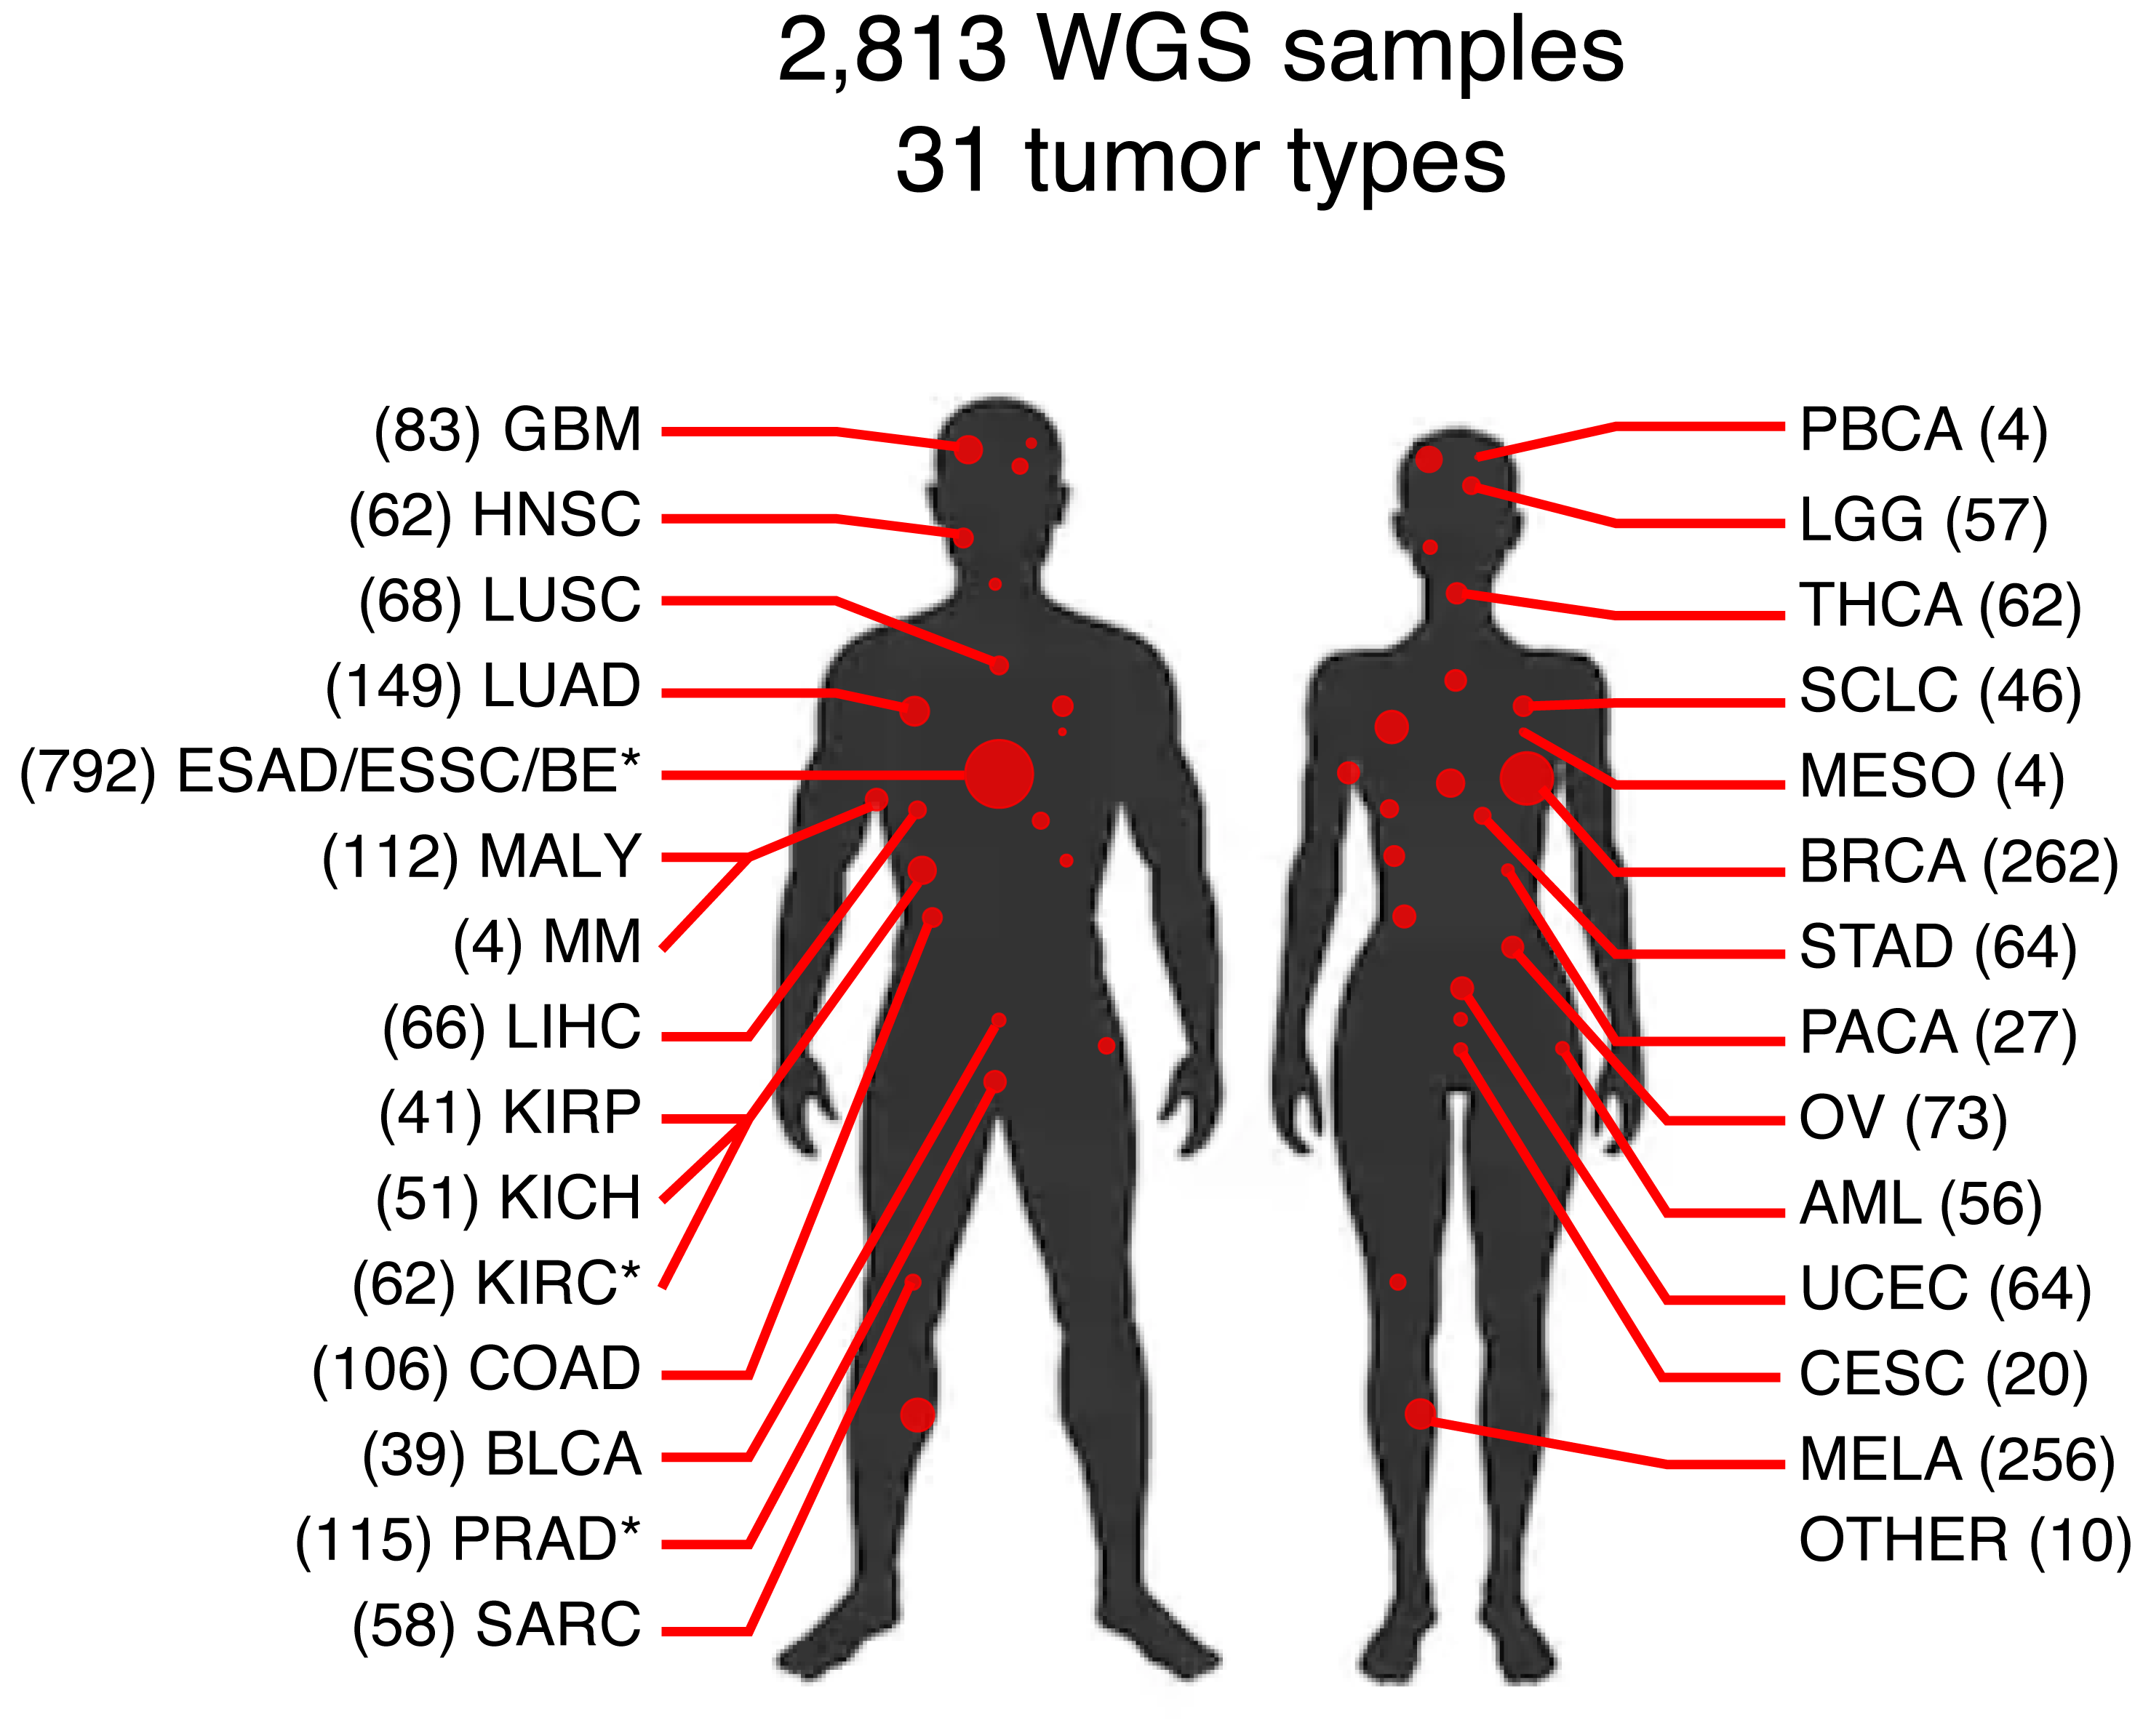
\includegraphics[width=0.95\linewidth]{figures/600ppi/pancancer.png}
    \caption{\textbf{Pan-cancer WGS tumor types.}}
    \label{fig:pancancer}
\end{figure*}

\begin{figure*}
    \centering
    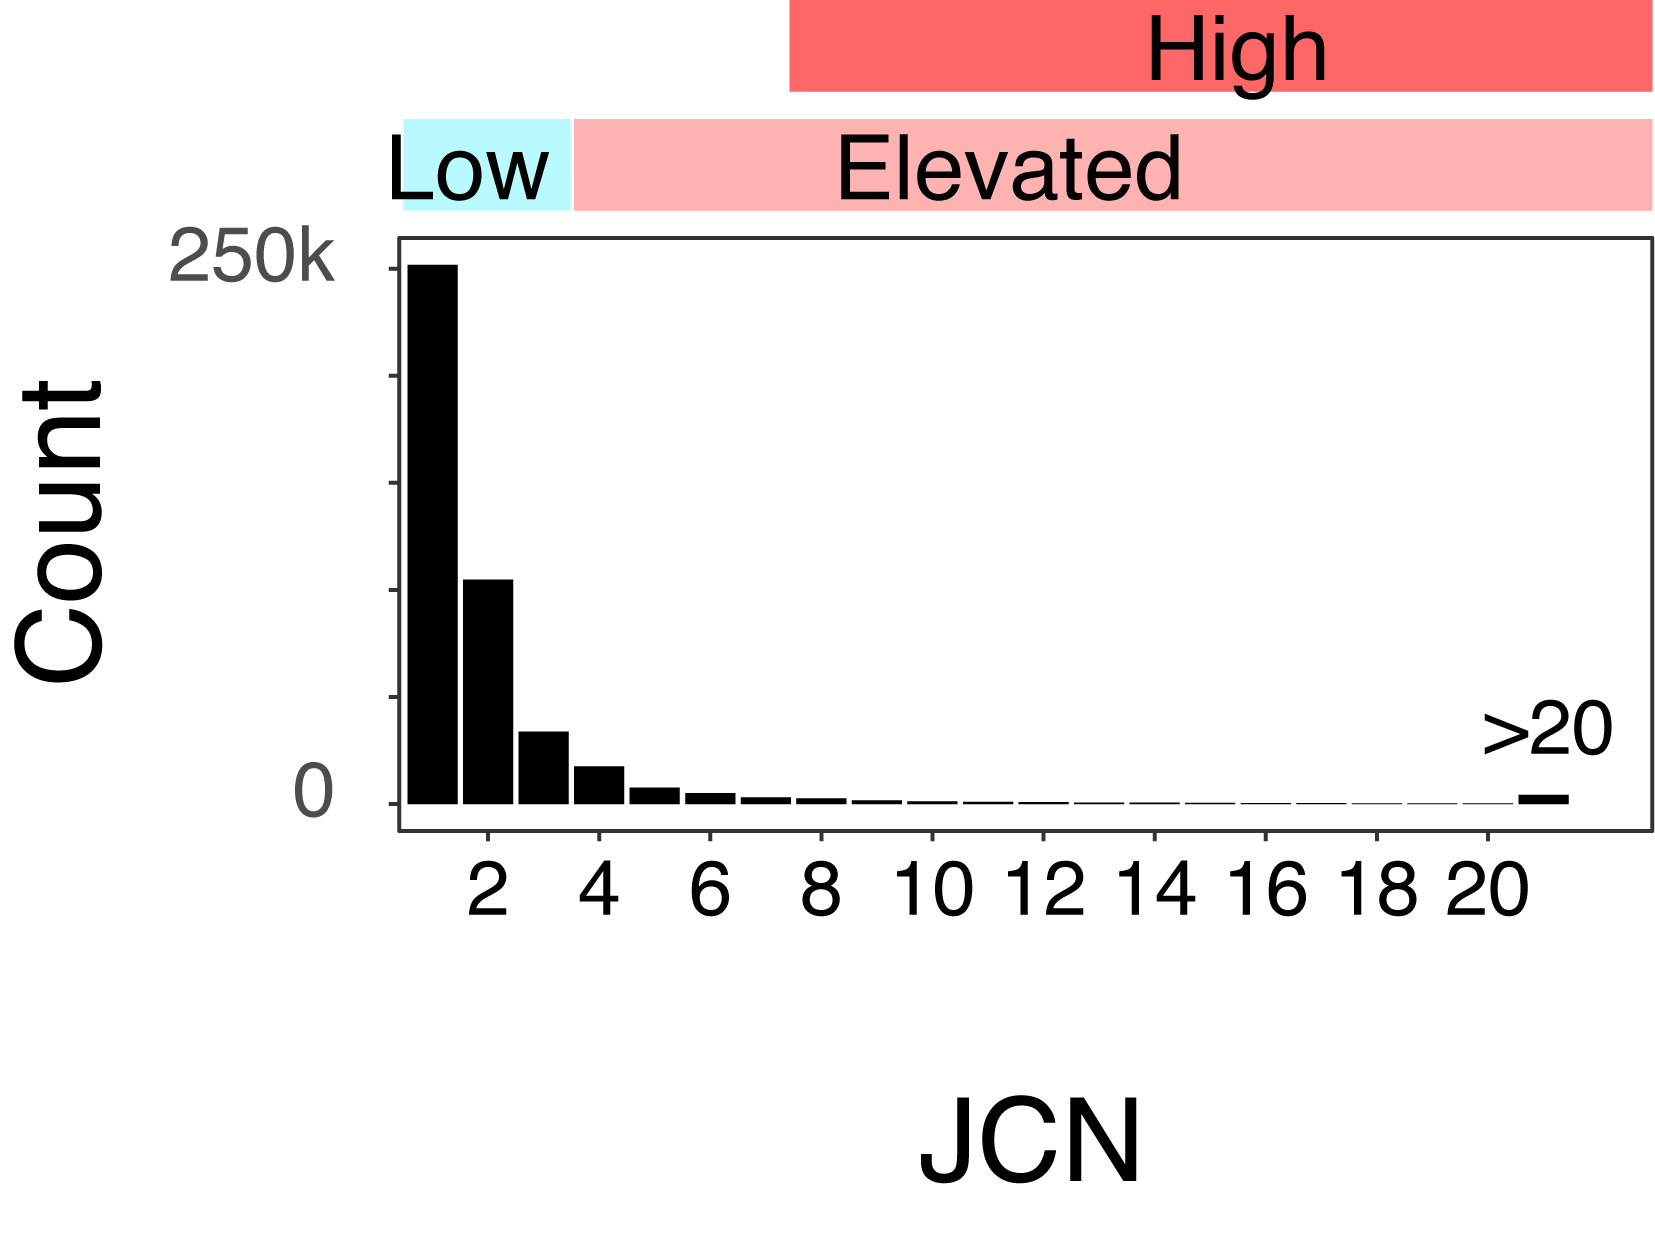
\includegraphics[width=0.95\linewidth]{figures/600ppi/jcn_hist.png}
    \caption{\textbf{Pan-cancer junction copy number (JCN) distribution.}}
    \label{fig:jcn_hist}
\end{figure*}

\begin{figure*}
    \centering
    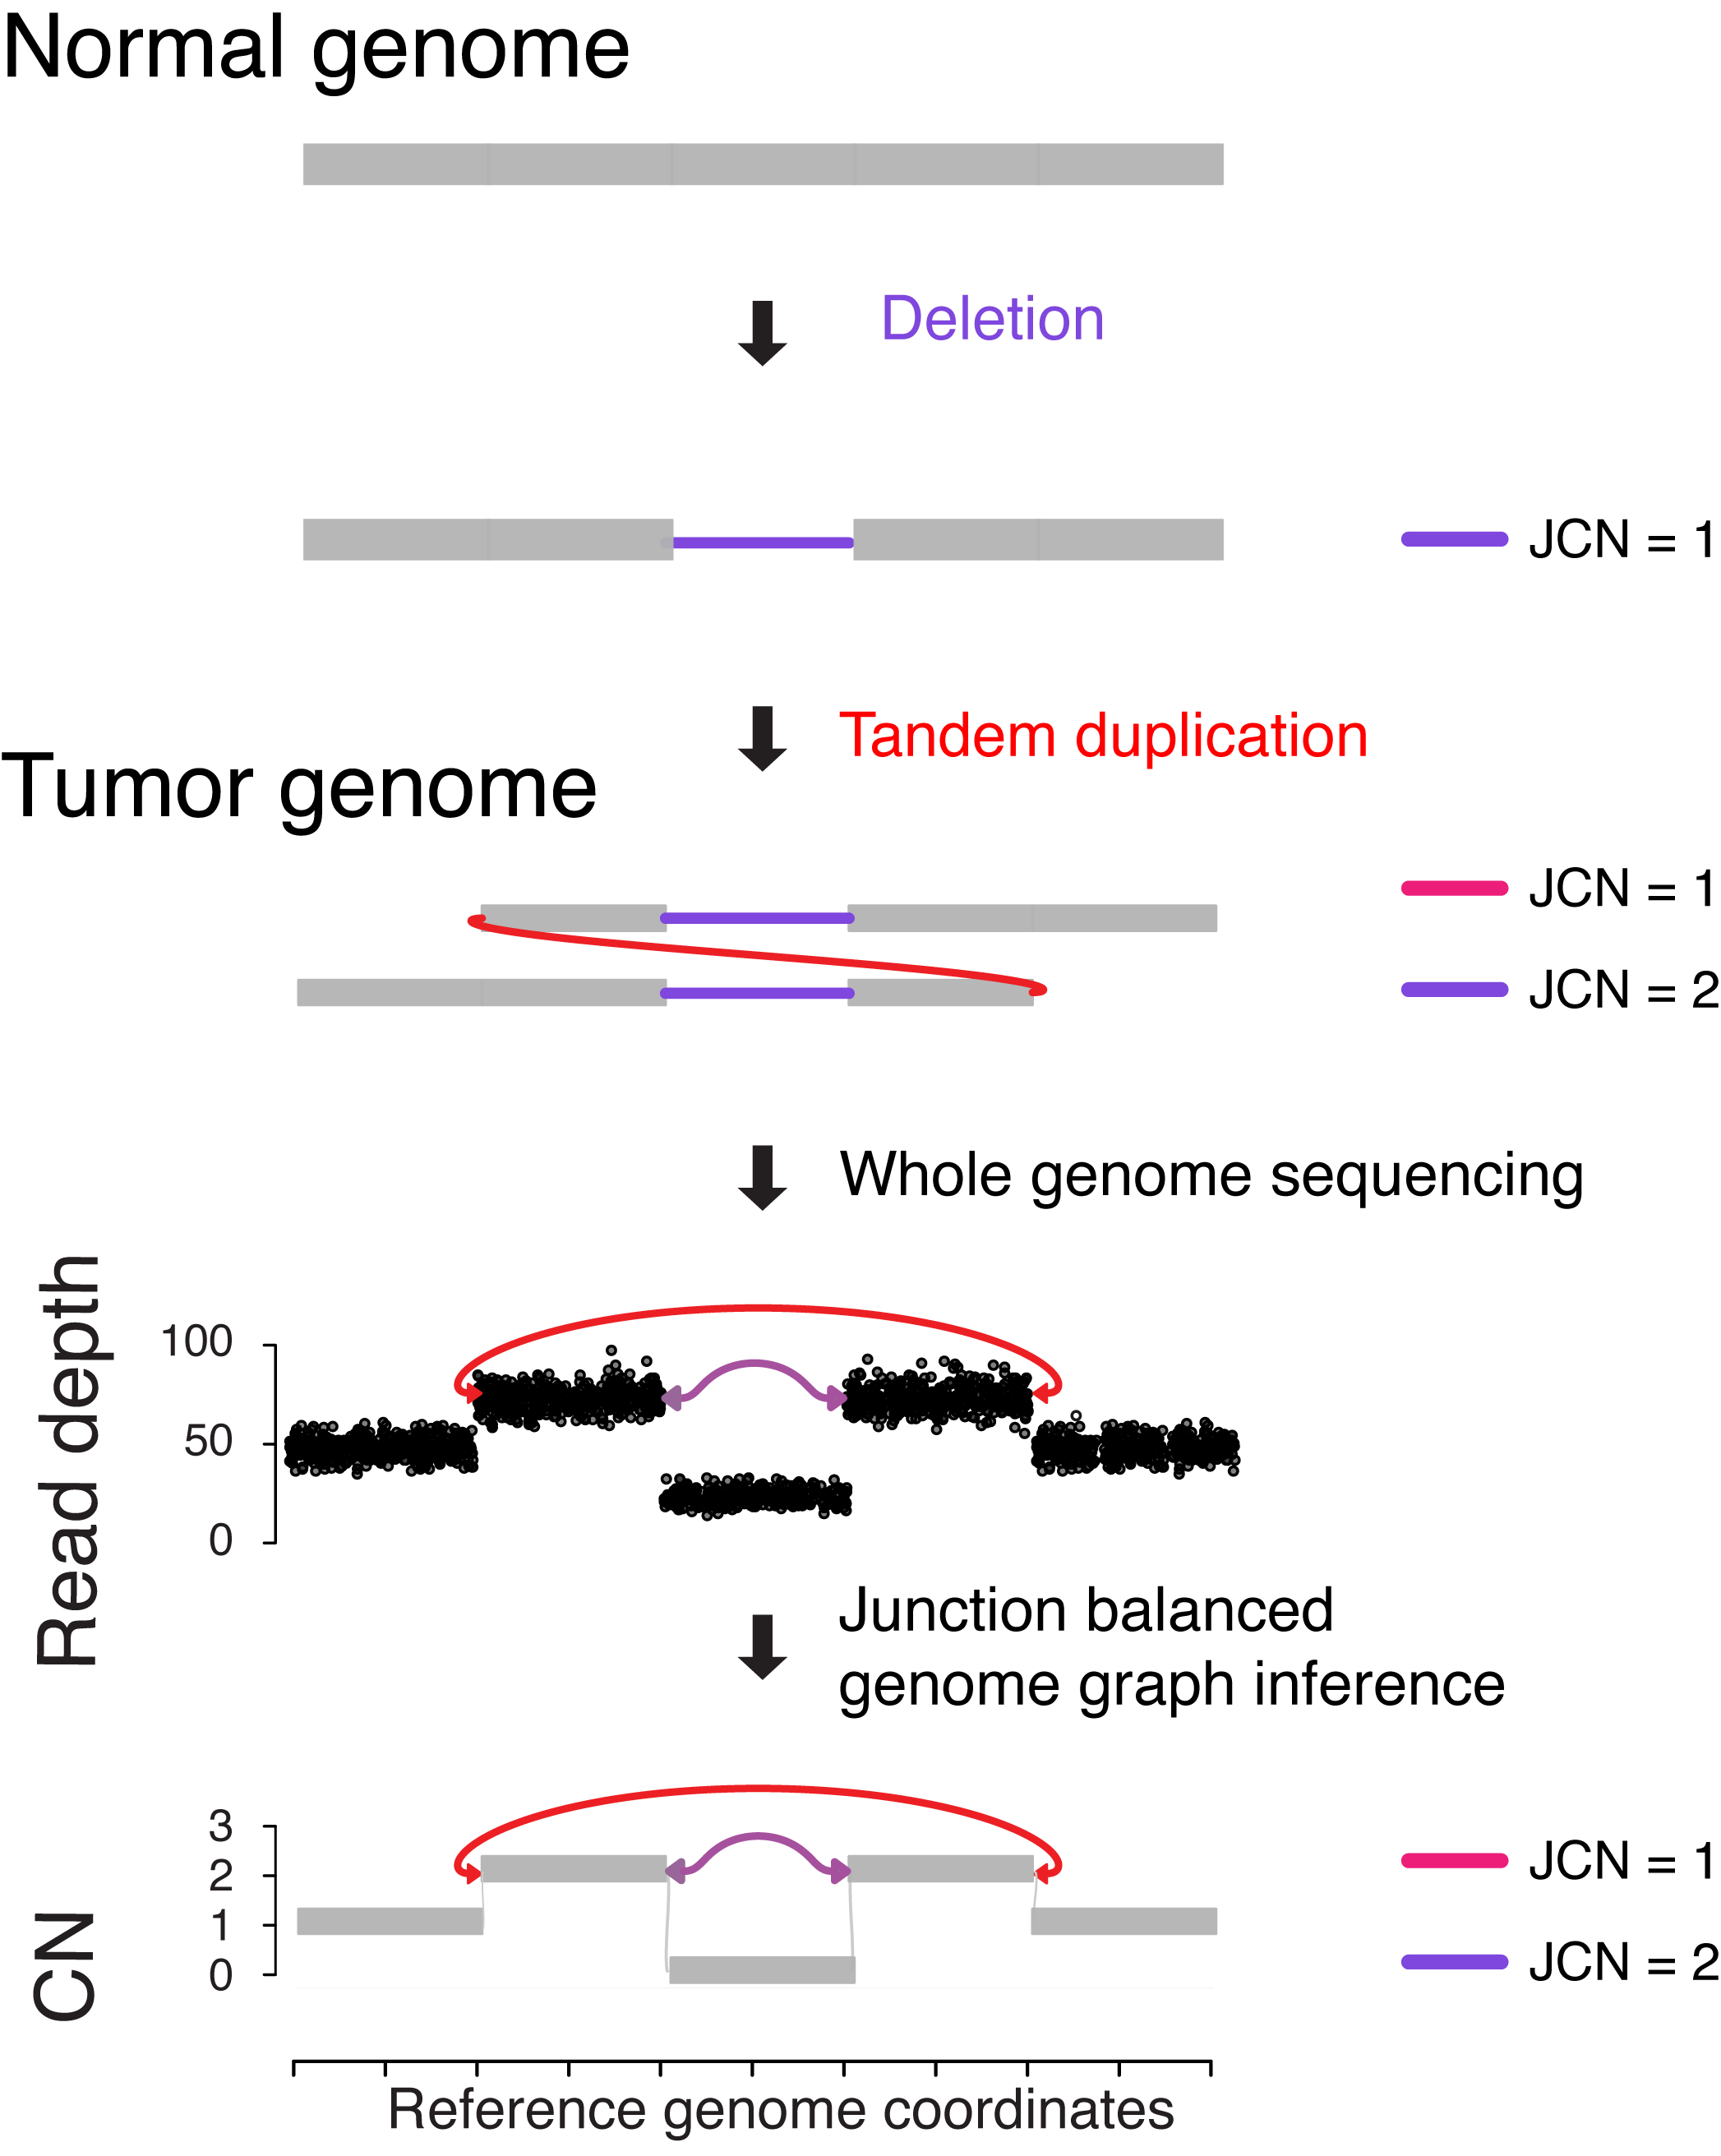
\includegraphics[width=0.95\linewidth]{figures/600ppi/jcn.png}
    \caption{\textbf{Illustration of JCN.}}
    \label{fig:jcn}
\end{figure*}

\begin{figure*}
    \centering
    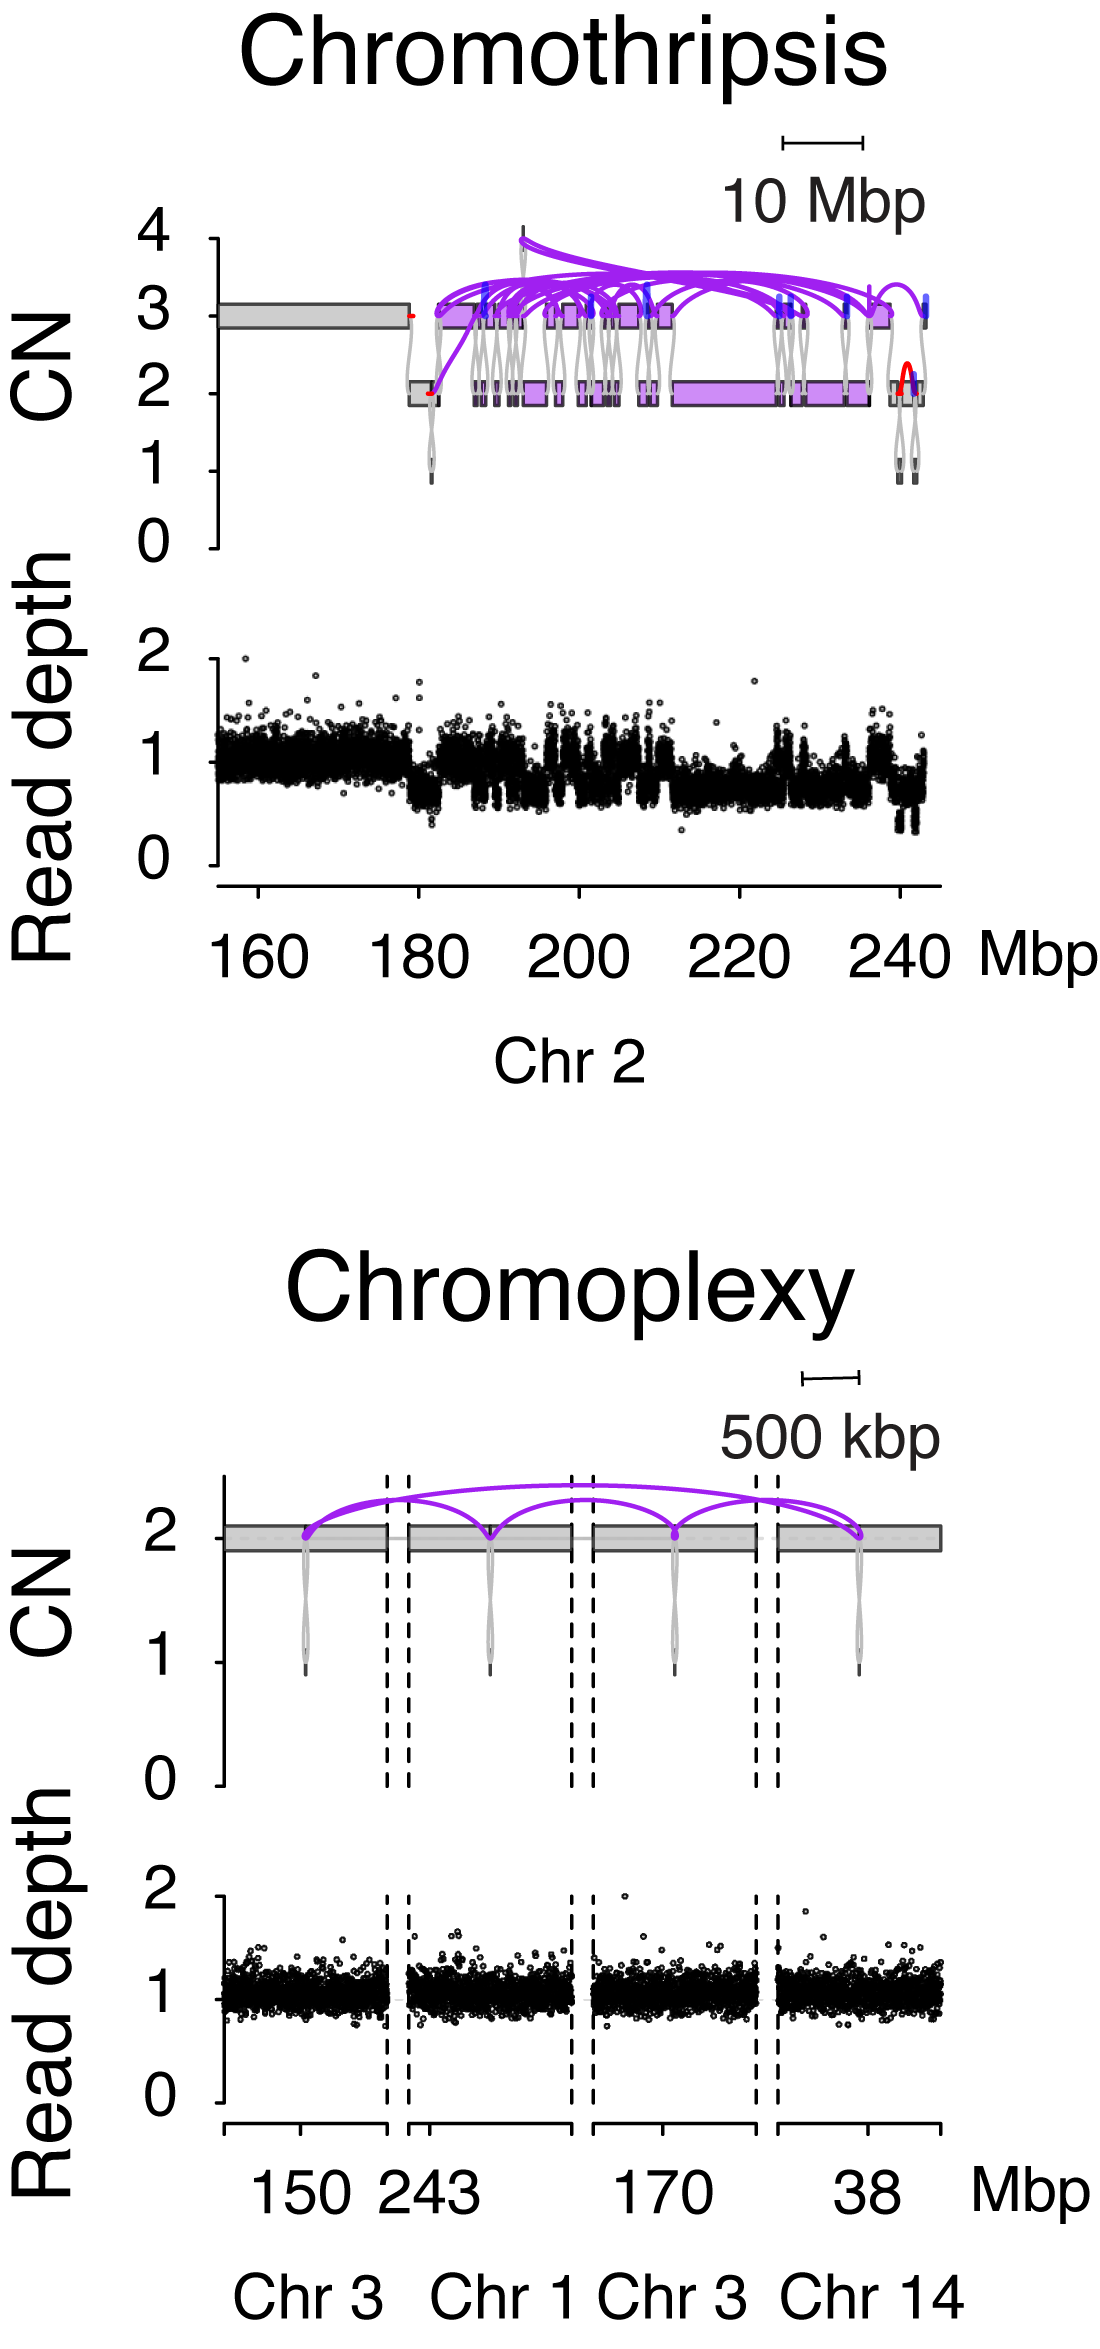
\includegraphics[height=0.95\textheight]{figures/600ppi/variant_subgraph.png}
    \caption{\textbf{Example of chromothripsis and chromoplexy.}}
    \label{fig:variant_subgraph}
\end{figure*}

\begin{figure}
    \centering
    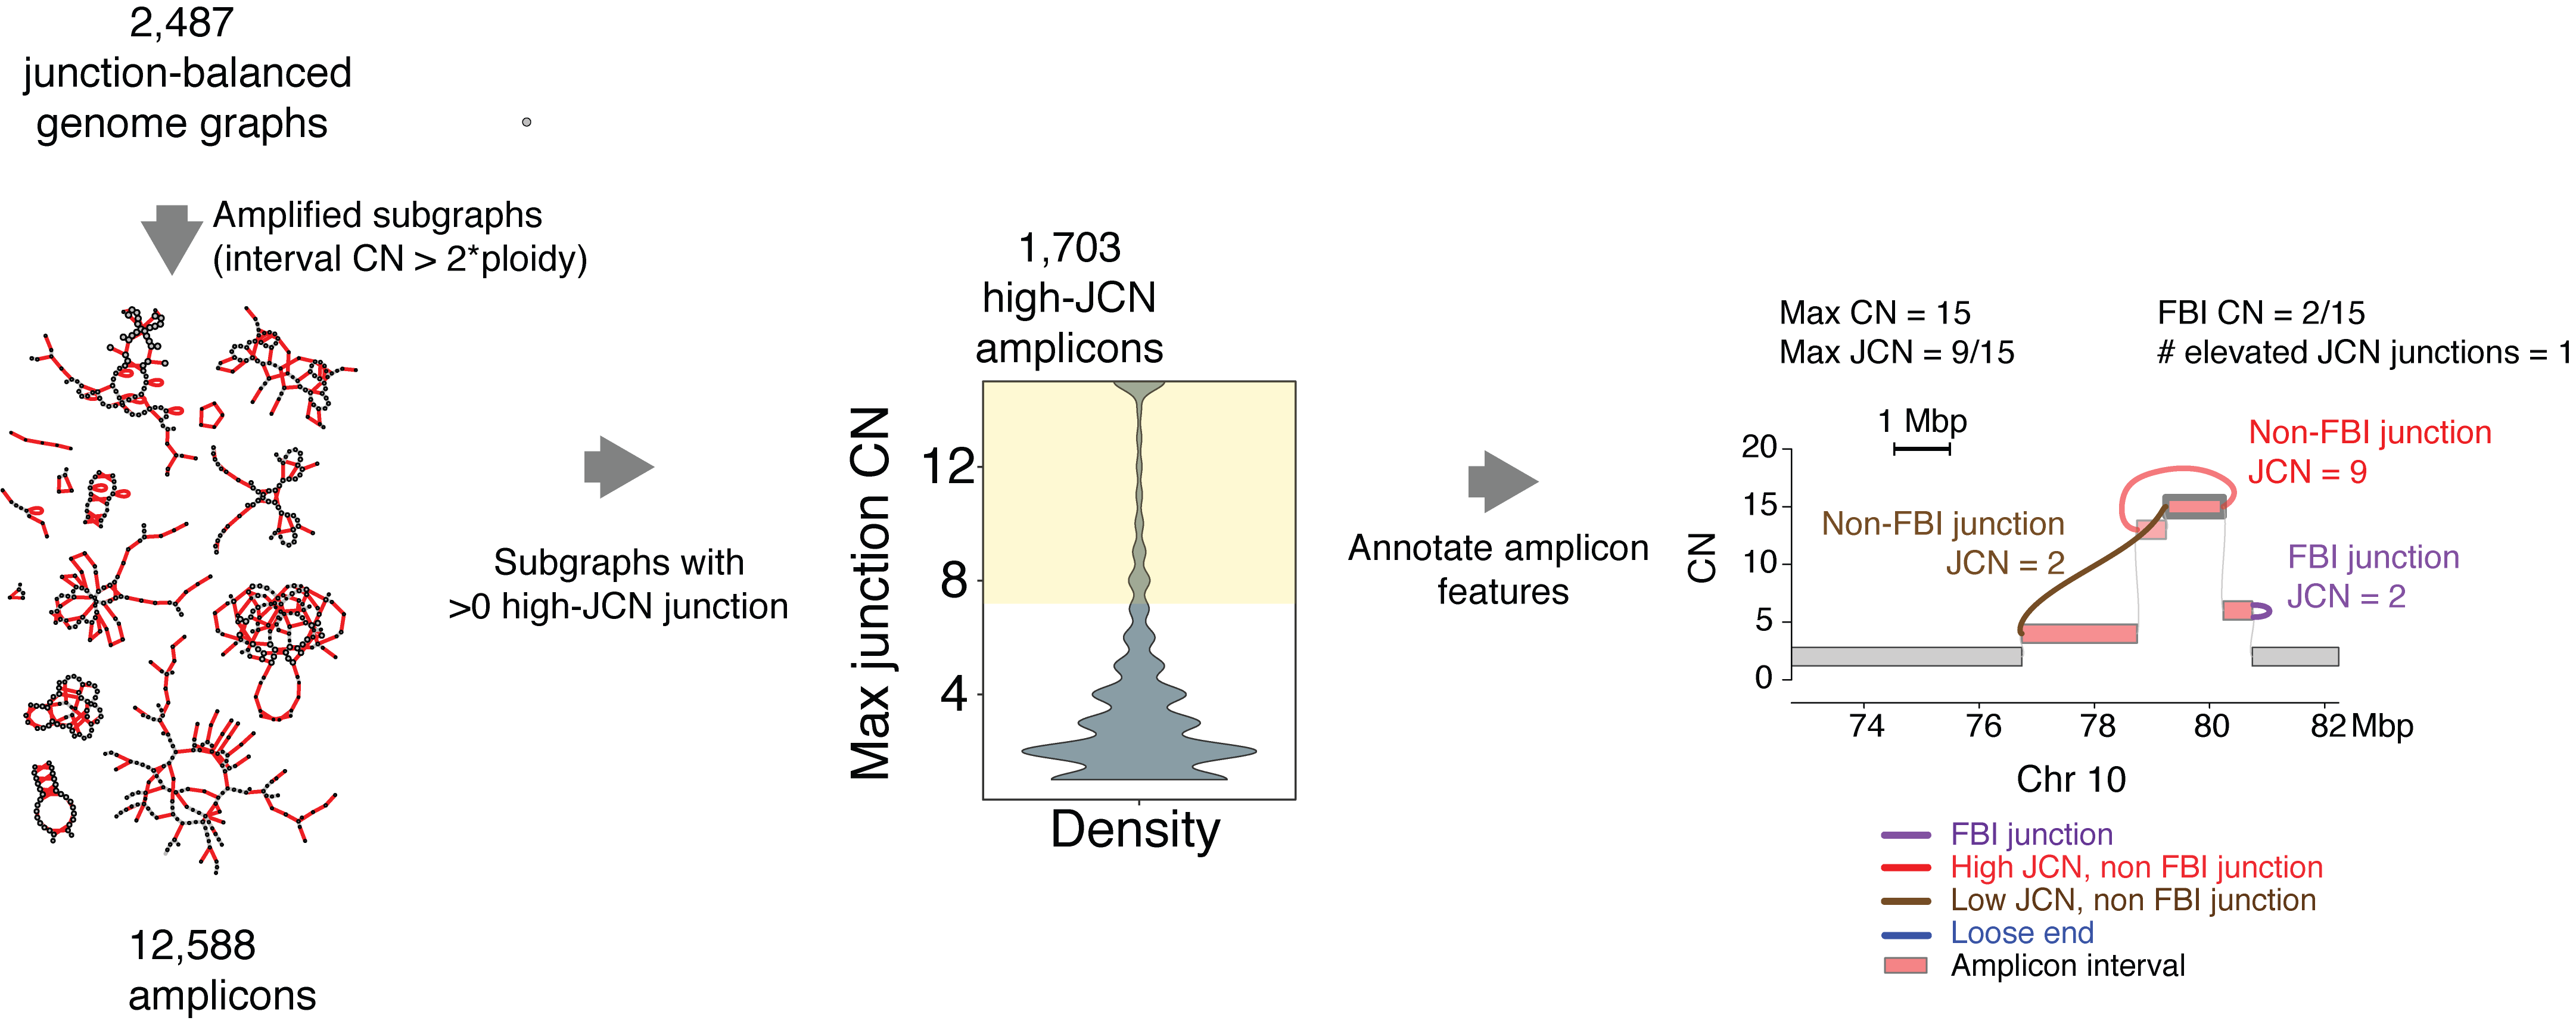
\includegraphics[width=0.95\linewidth]{figures/600ppi/amplicon.png}
    \caption{\textbf{Candidate amplicon subgraphs and the feature space construction.}}
    \label{fig:amplicon_features}
\end{figure}

\begin{figure*}
    \centering
    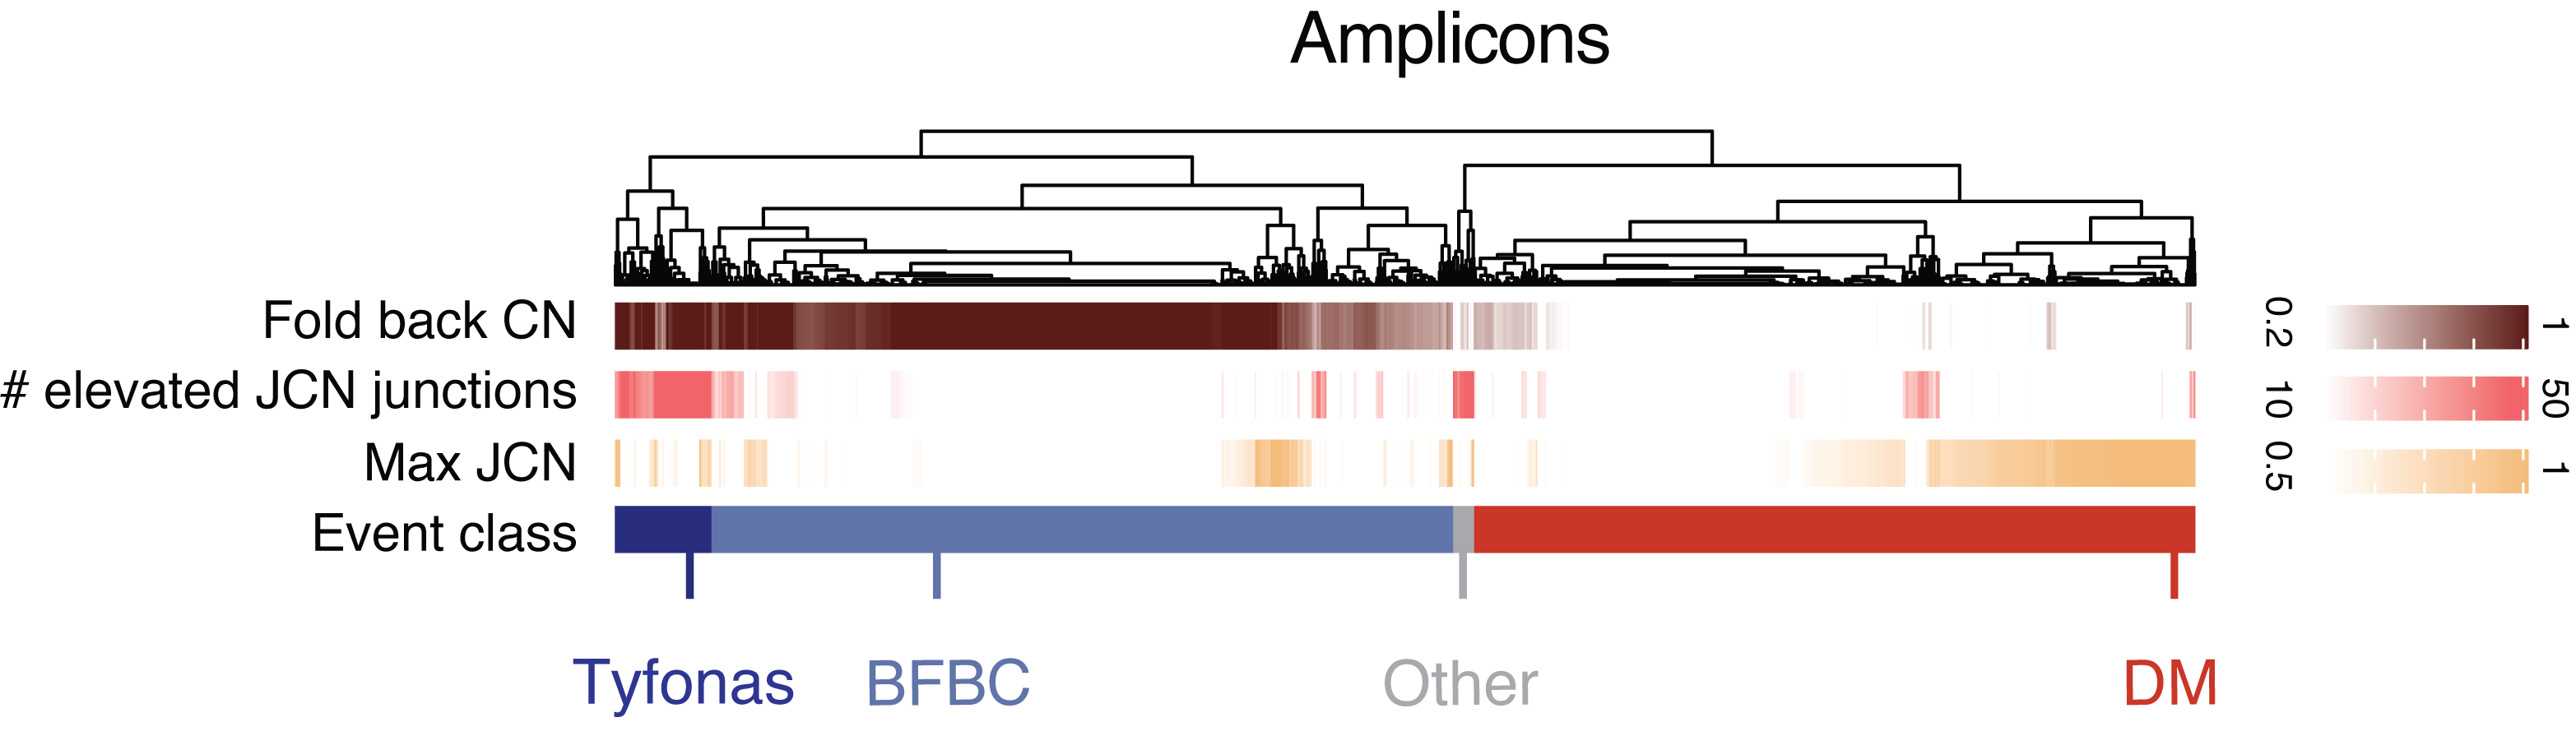
\includegraphics[width=0.95\linewidth]{figures/600ppi/amplicon_clustering.png}
    \label{fig:amplicon_definition}
    \caption{\textbf{Classification of amplicons with high-JCN junctions.}}
\end{figure*}

\begin{figure*}
    \centering
    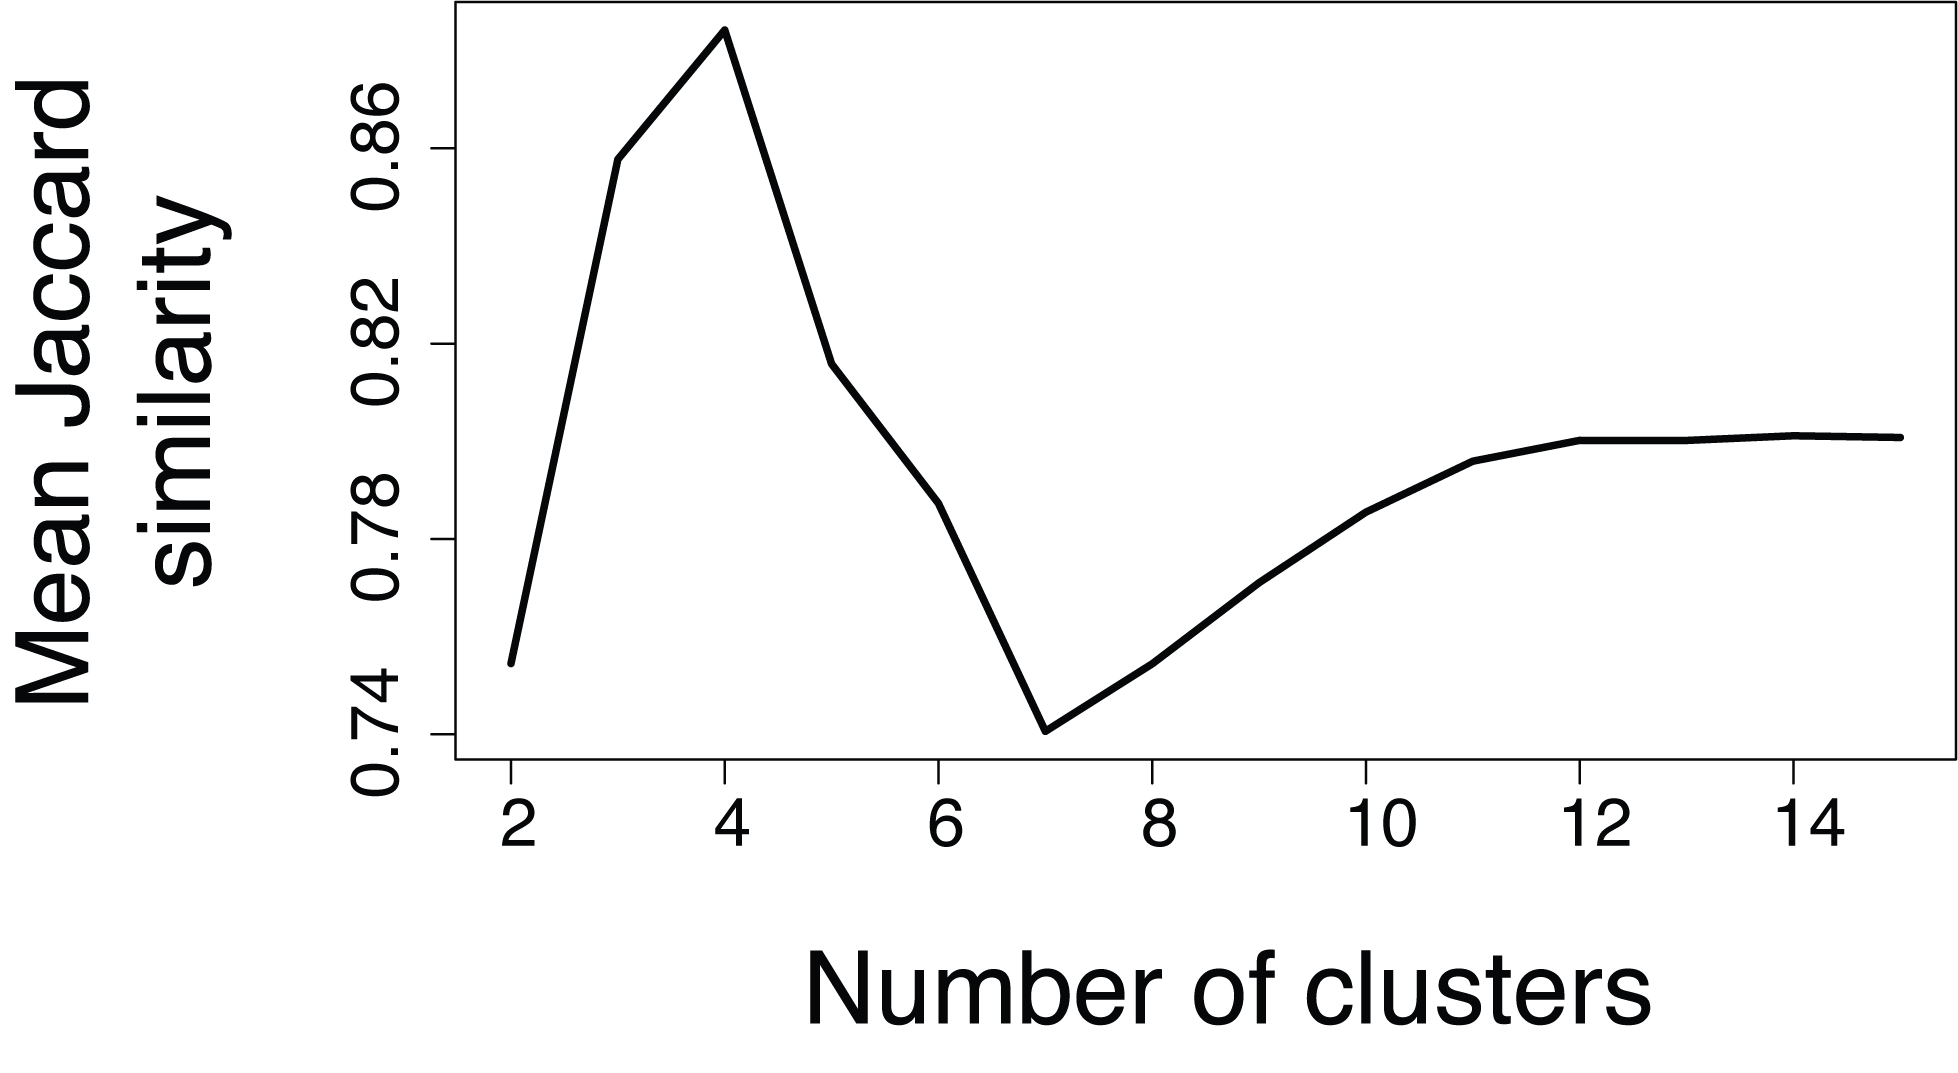
\includegraphics[width=0.95\linewidth]{figures/600ppi/amplicon_clustering_jaccard.png}
    \label{fig:amplicon_jaccard}
    \caption{\textbf{Assessment of stability of amplicon clustering.}}{For a given setting of $k$, cluster stability was computed as the mean Jaccard similarity between each observed cluster and the most similar cluster across 100 75\% bootstraps of the data (see \nameref{app:b}). The stability of each $k$ parameter setting was computed as the mean of the $k$ stability scores across the clusters generated at that setting.}
\end{figure*}

\begin{figure*}
    \centering
    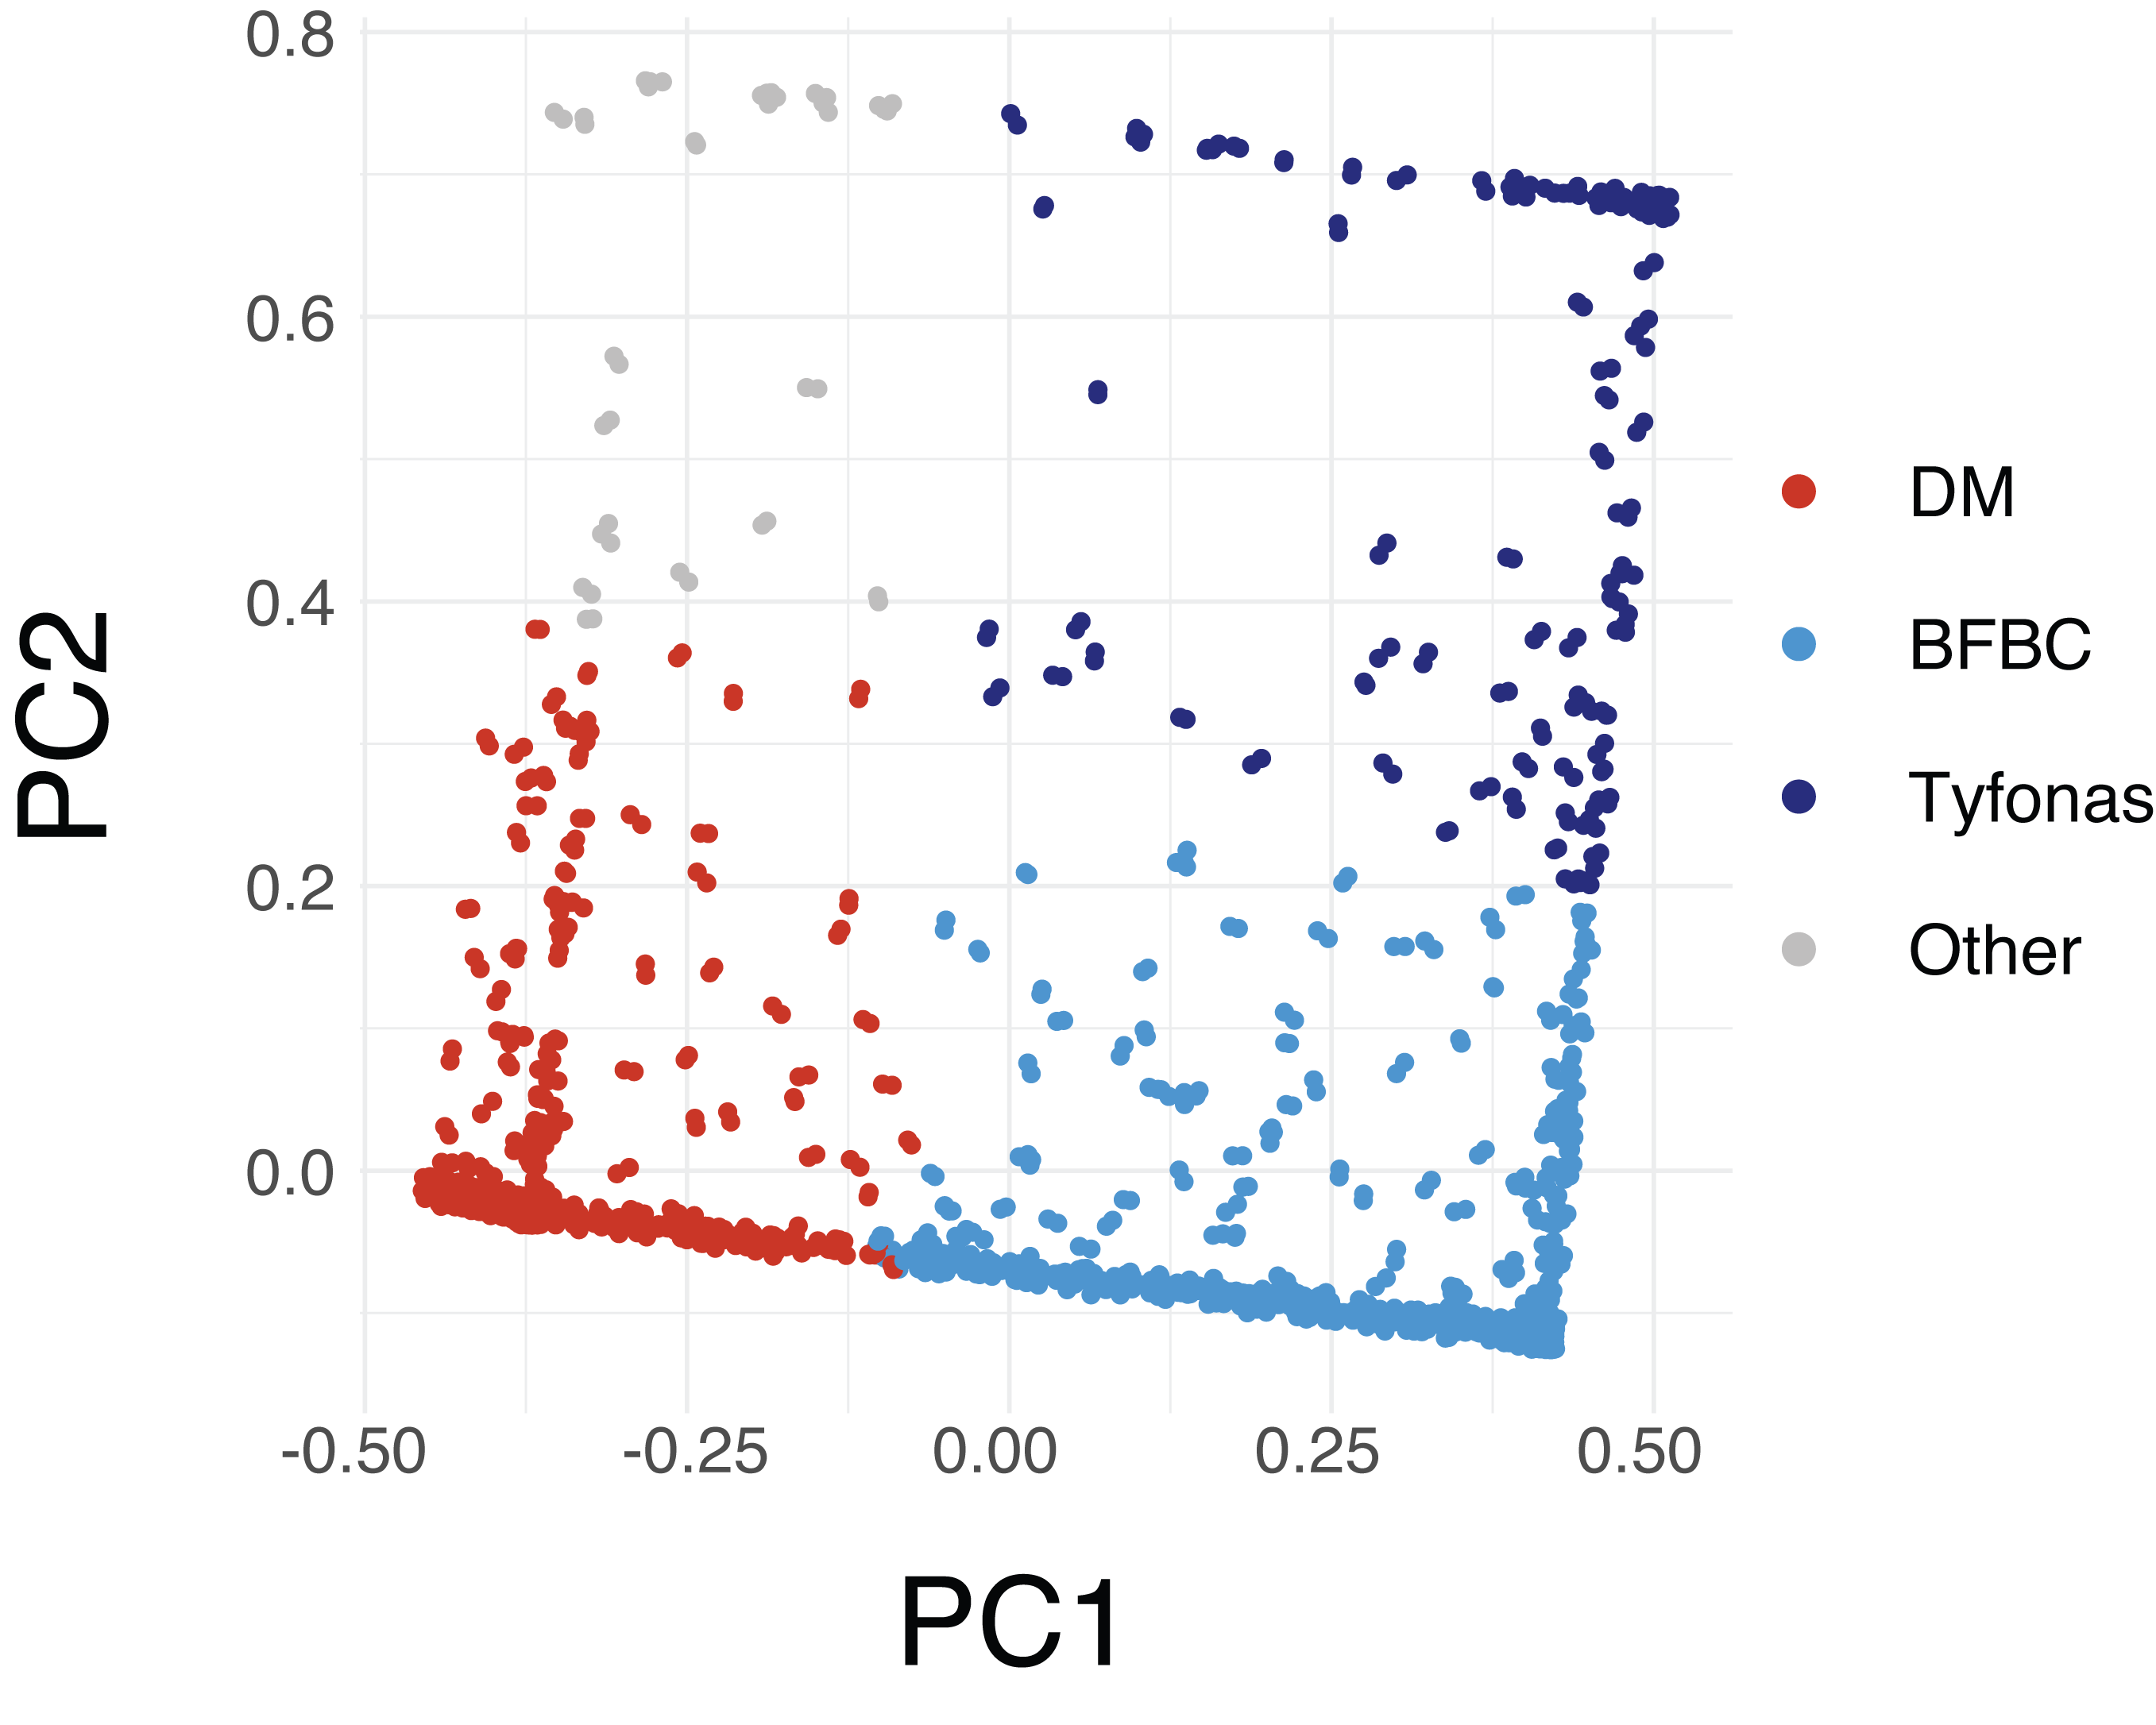
\includegraphics[width=0.95\linewidth]{figures/600ppi/amplicon_pca.png}
    \label{fig:amplicon_pca}
    \caption{\textbf{Projection of the amplicons across the first two principal components of normalized amplicon features.}}{}
\end{figure*}

\begin{figure*}
    \centering
    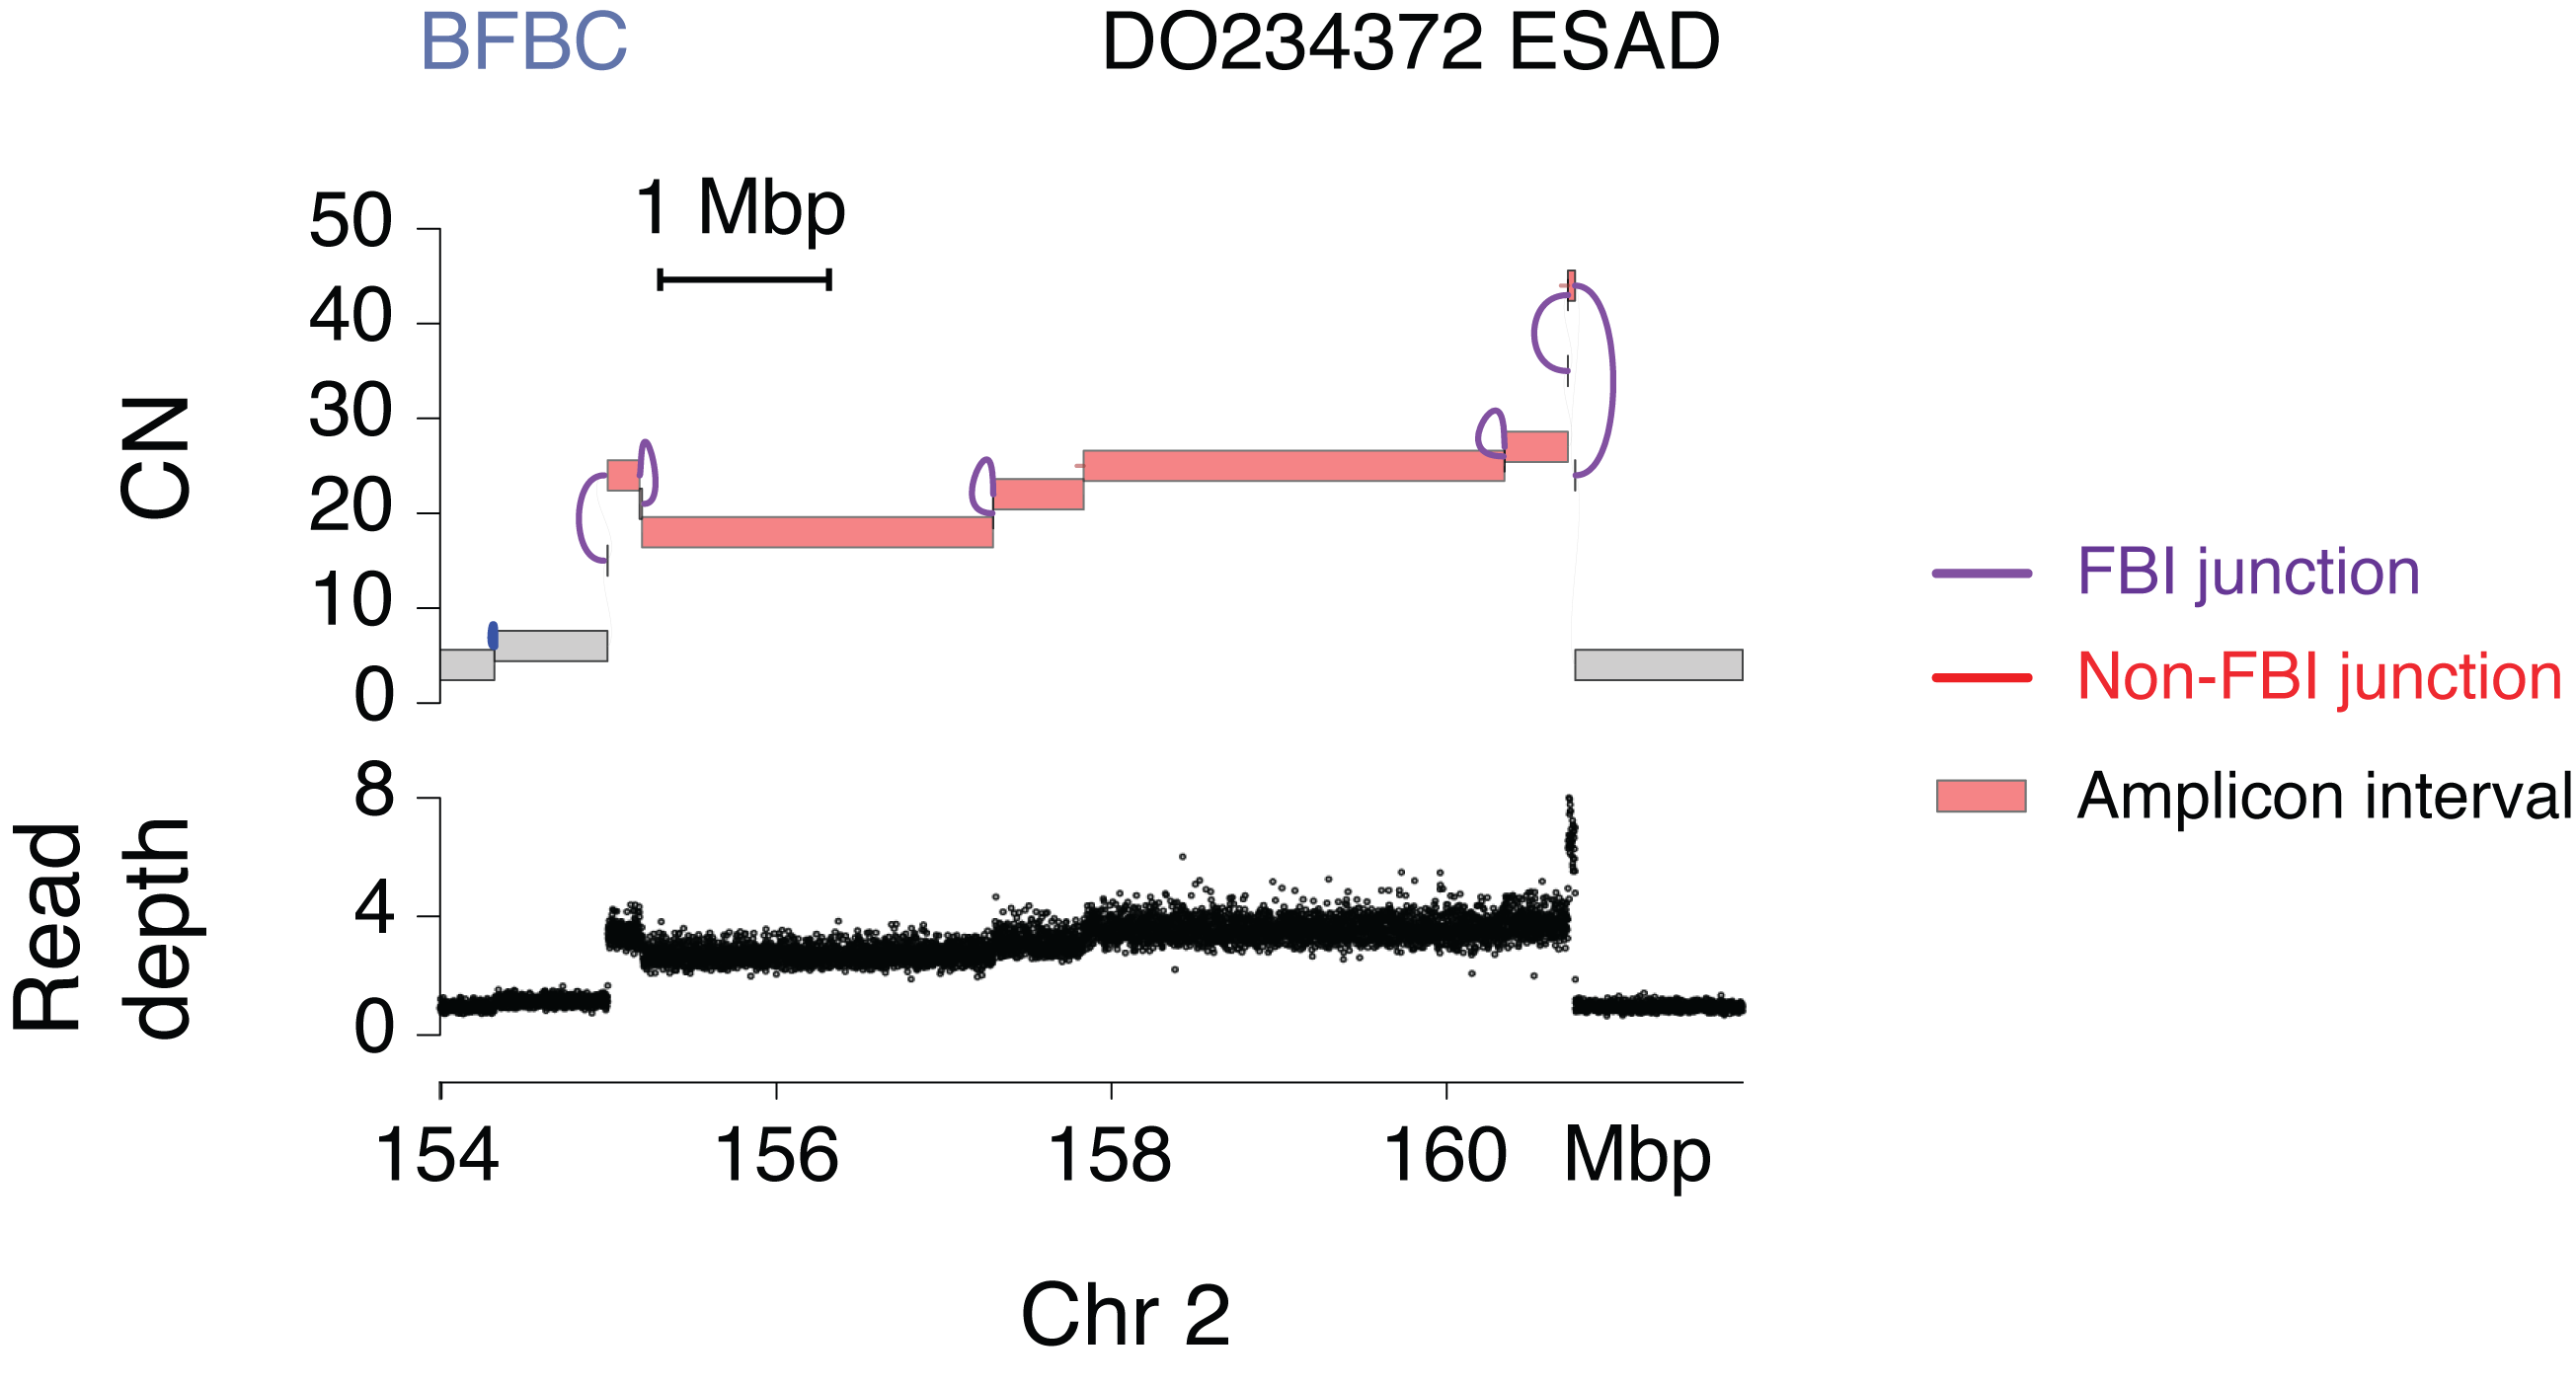
\includegraphics[width=0.95\linewidth]{figures/600ppi/bfb_example.png}
    \label{fig:bfb_example}
    \caption{\textbf{An example of a BFB cycles pattern.}}
\end{figure*}

\begin{figure*}
    \centering
    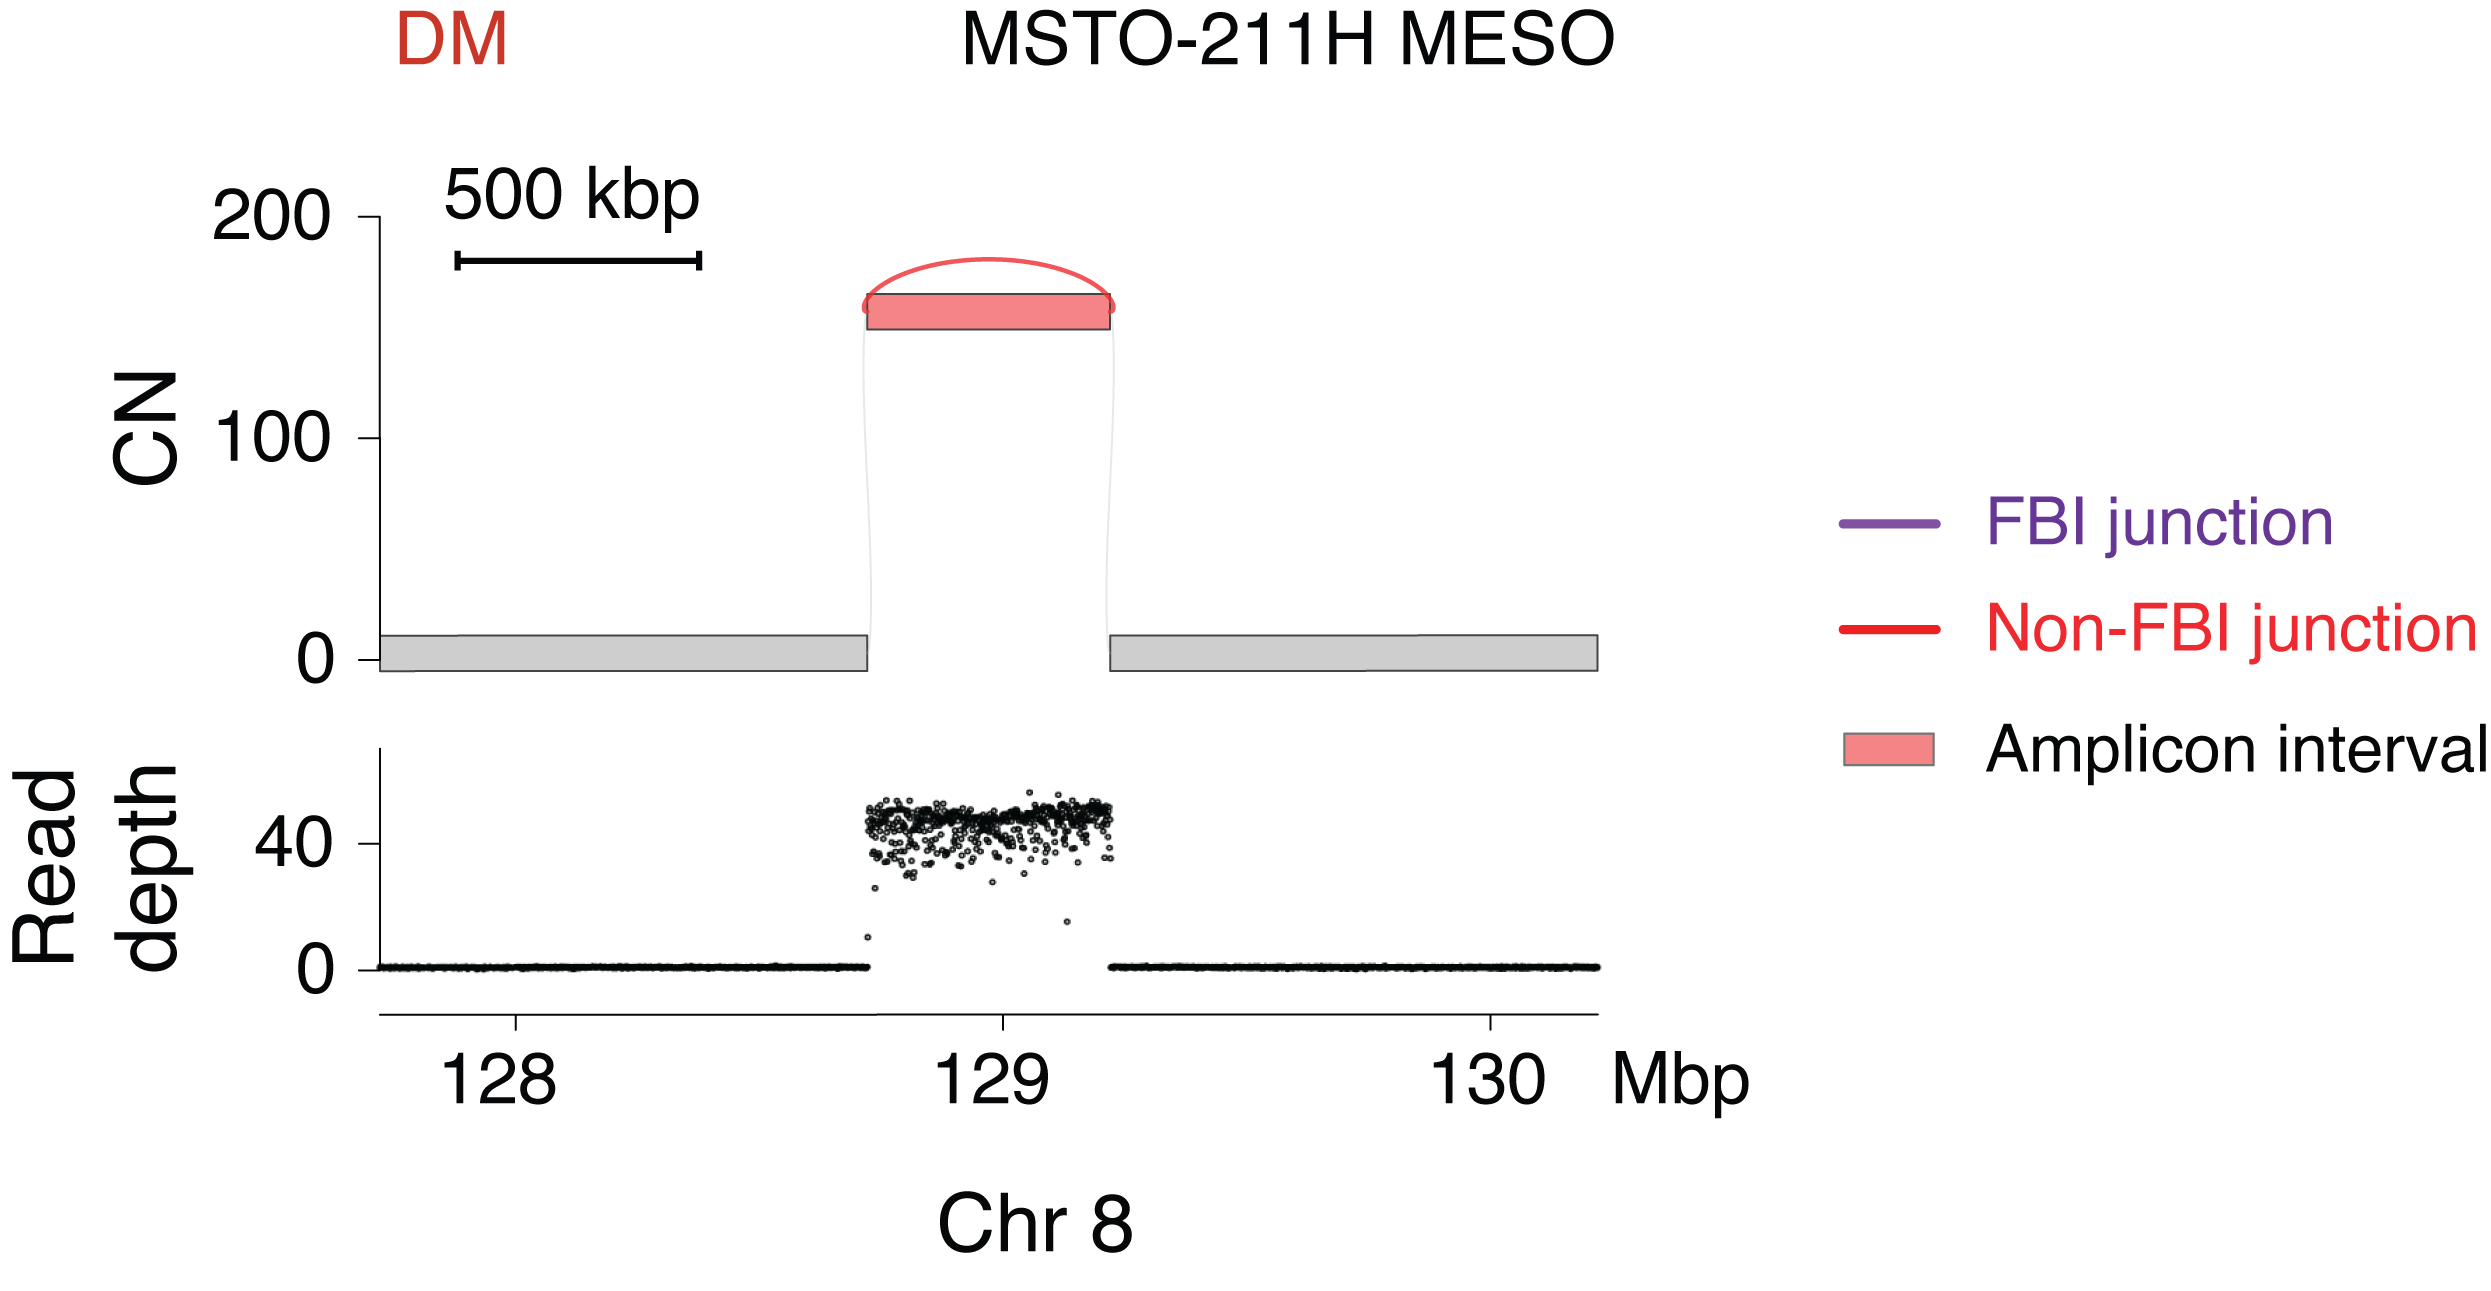
\includegraphics[width=0.95\linewidth]{figures/600ppi/dm_example.png}
    \label{fig:dm_example}
    \caption{\textbf{An example of a double minute pattern.}}
\end{figure*}

\begin{figure*}
    \centering
    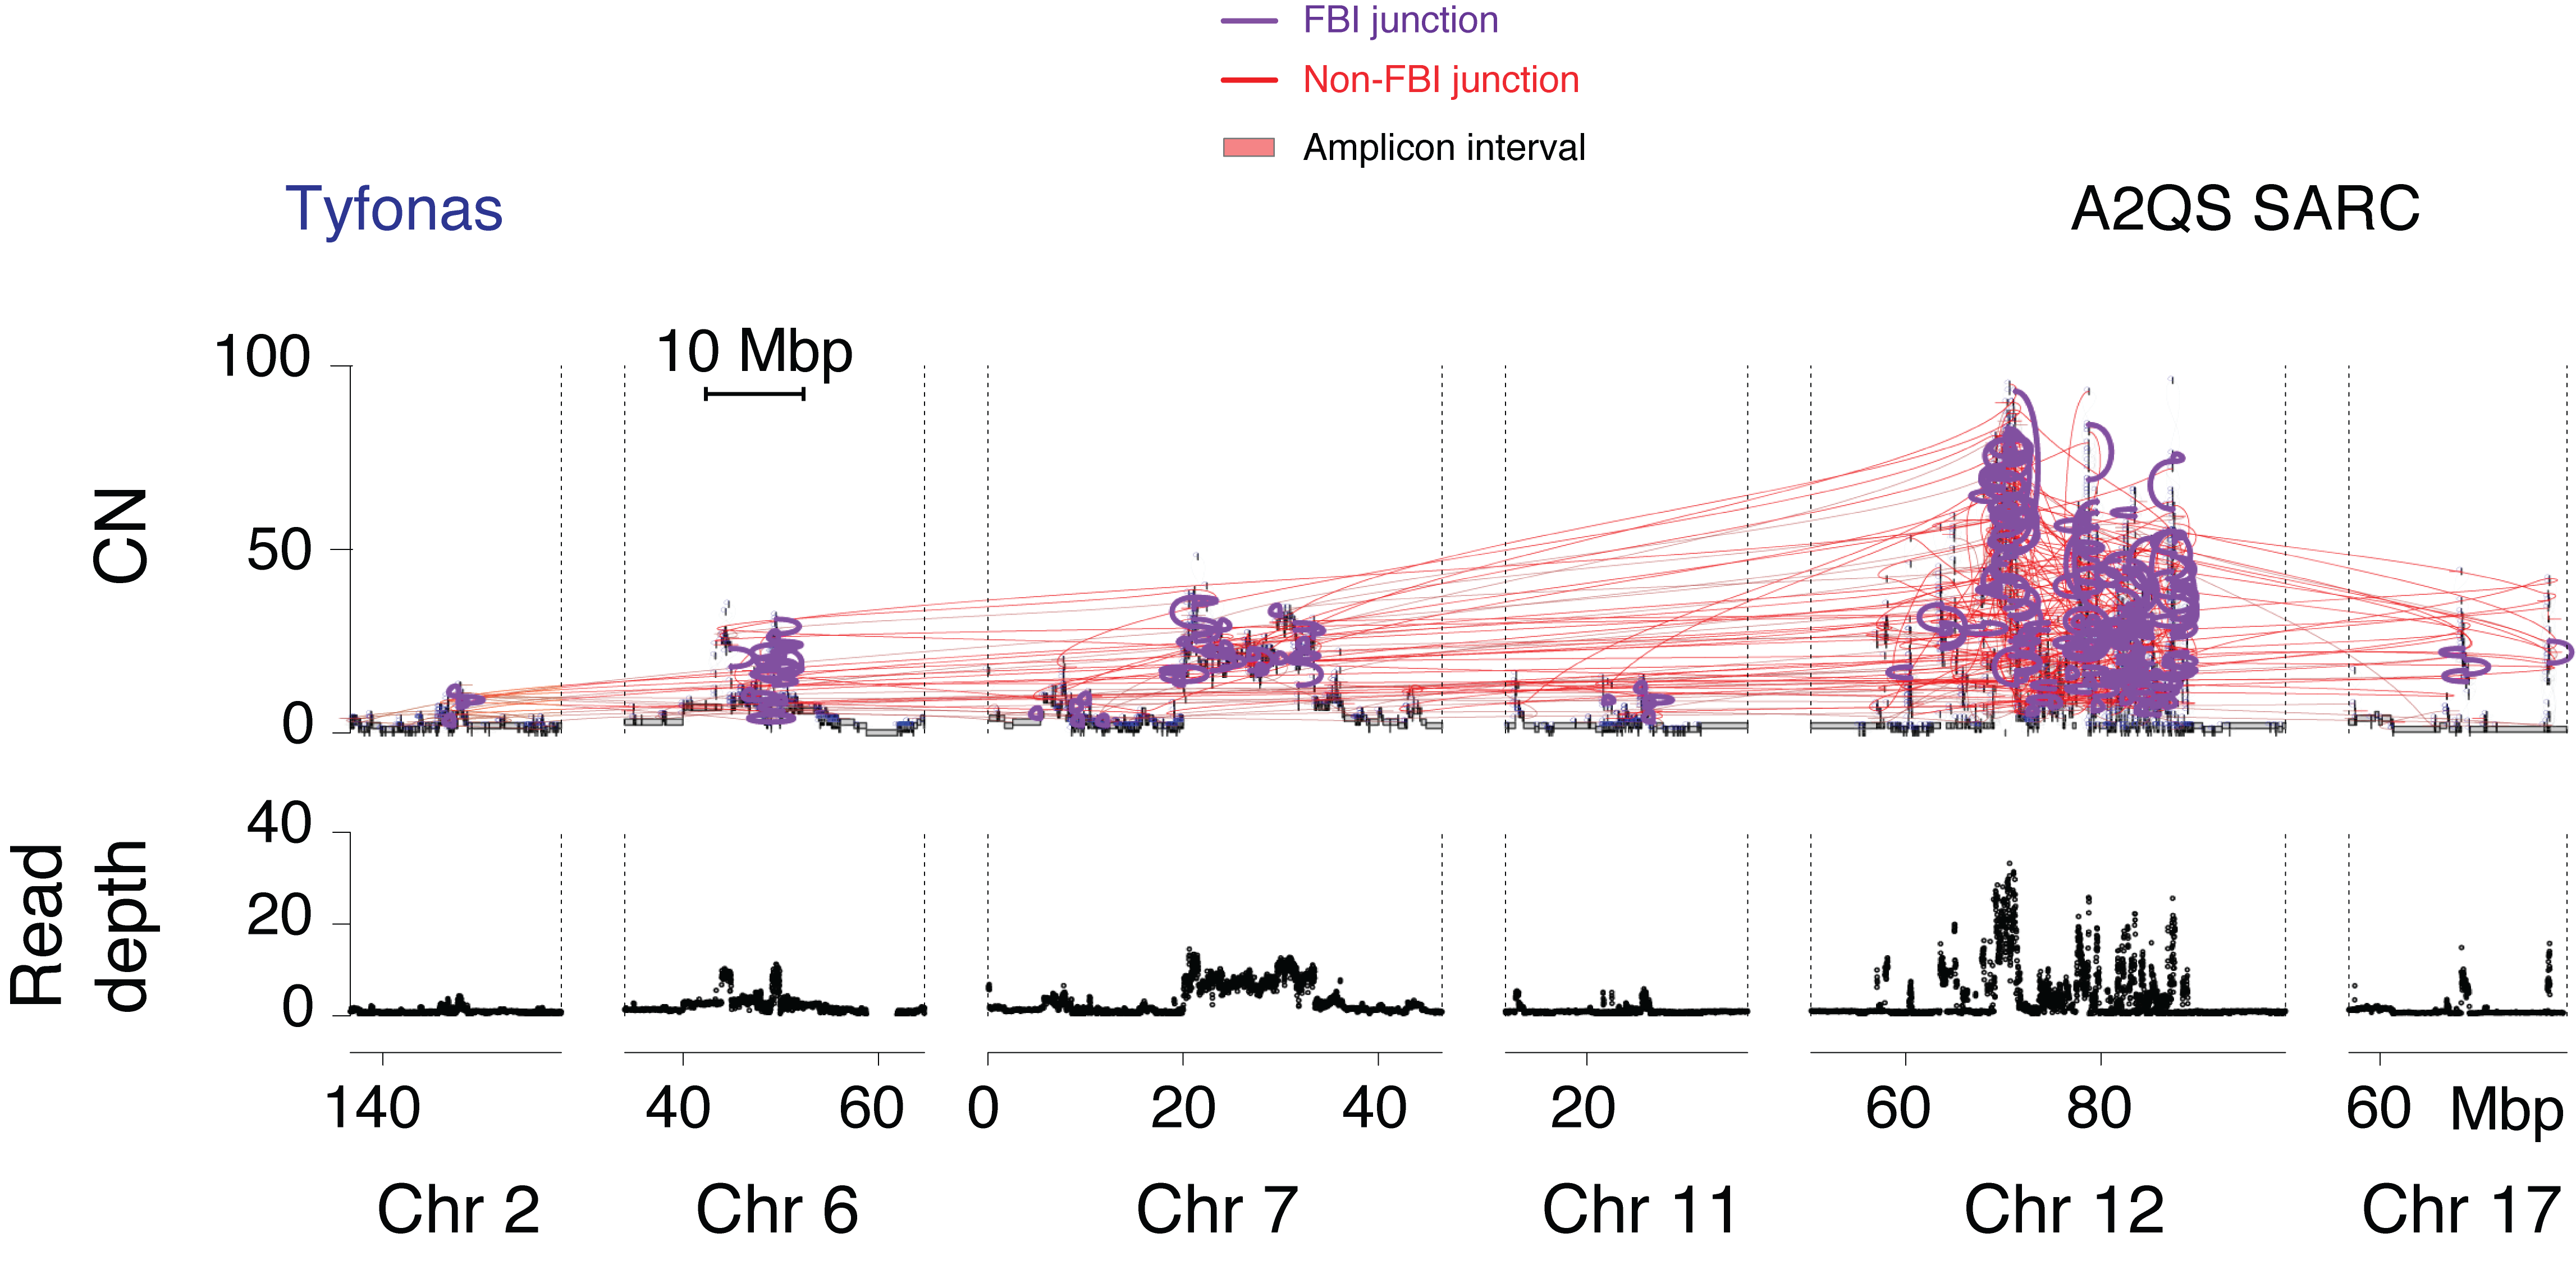
\includegraphics[width=0.95\linewidth]{figures/600ppi/tyf_example.png}
    \label{fig:tyf_example}
    \caption{\textbf{An example of a tyfonas pattern.}}
\end{figure*}

\begin{figure*}
    \centering
    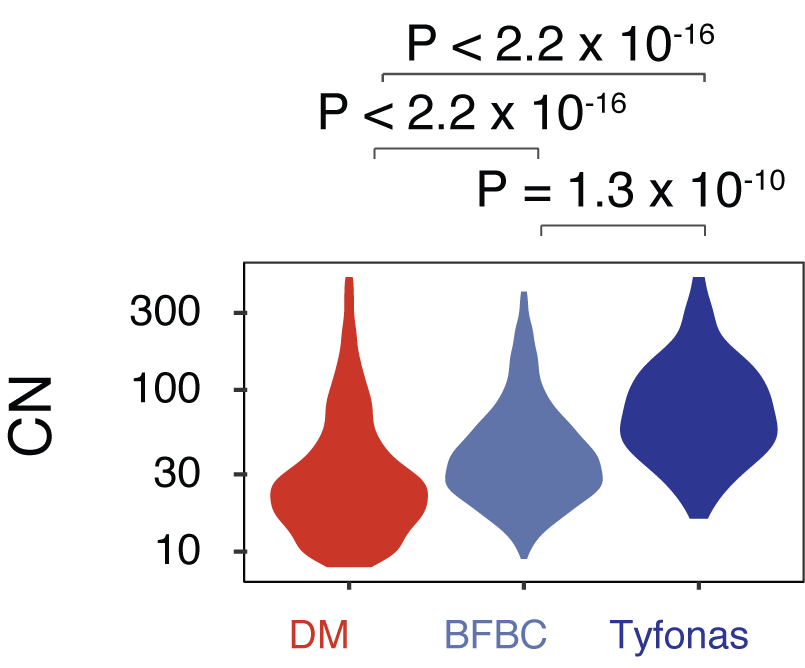
\includegraphics[width=0.95\linewidth]{figures/600ppi/amplicon_cn.png}
    \label{fig:amplicon_cn}
    \caption{\textbf{Tyfonas amplify parts of genome to higher CN states than BFB and DM.}}
\end{figure*}

\begin{figure*}
    \centering
    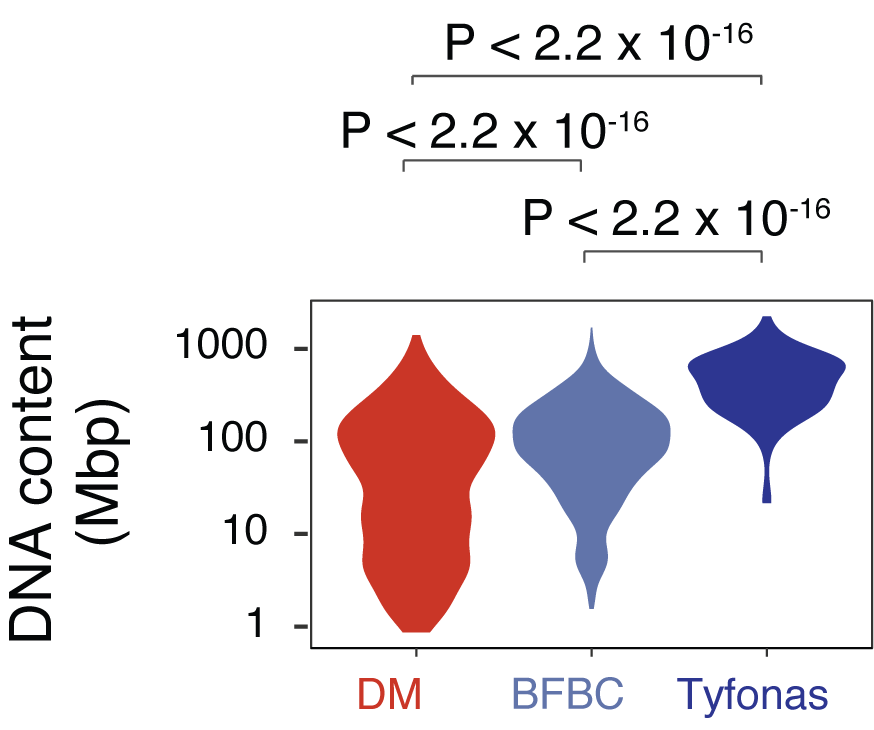
\includegraphics[width=0.95\linewidth]{figures/600ppi/amplicon_mass.png}
    \label{fig:amplicon_mass}
    \caption{\textbf{Tyfonas result in larger mass of amplified genomic DNA than BFB and DM.}}
\end{figure*}

\begin{figure*}
    \centering
    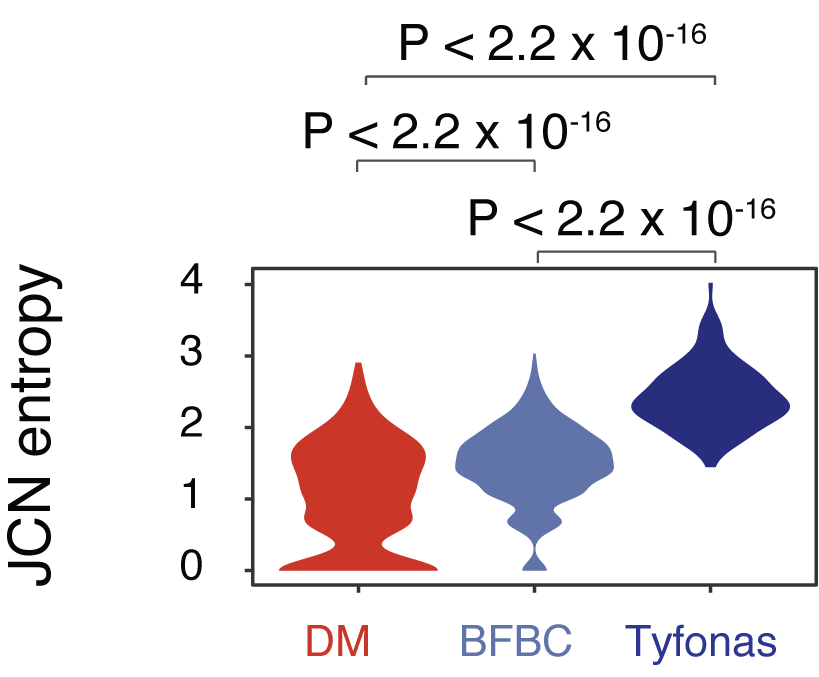
\includegraphics[width=0.95\linewidth]{figures/600ppi/amplicon_jcn_entropy.png}
    \label{fig:amplicon_jcn_entropy}
    \caption{\textbf{Tyfonas contain more heterogeneous junction copy numbers than BFB and DM.}}
\end{figure*}

\begin{figure*}
    \centering
    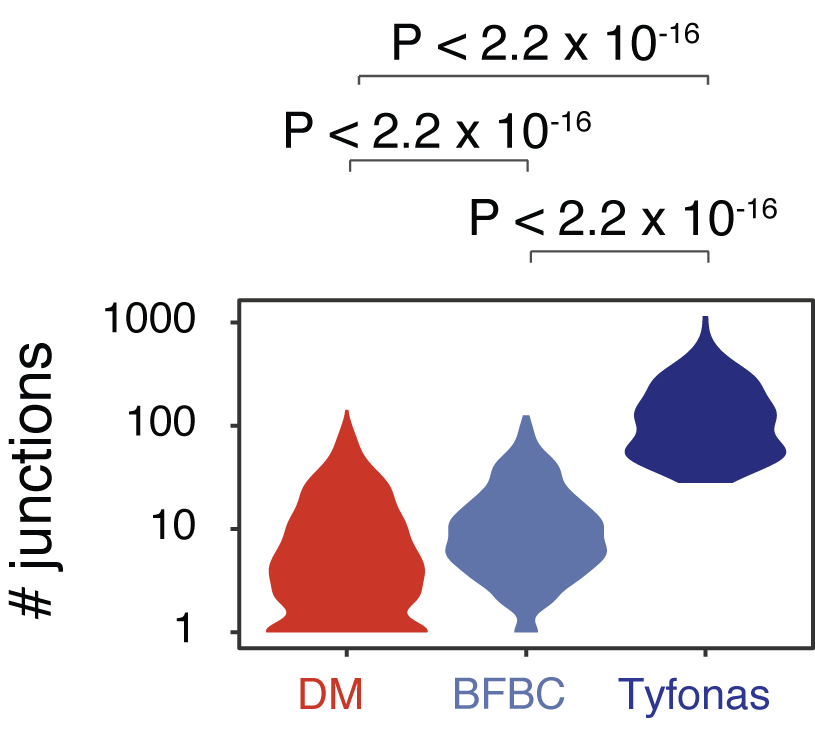
\includegraphics[width=0.95\linewidth]{figures/600ppi/amplicon_njunc.png}
    \label{fig:amplicon_njunc}
    \caption{\textbf{Tyfonas contain more junctions than BFB and DM.}}
\end{figure*}

\begin{figure}
    \centering
    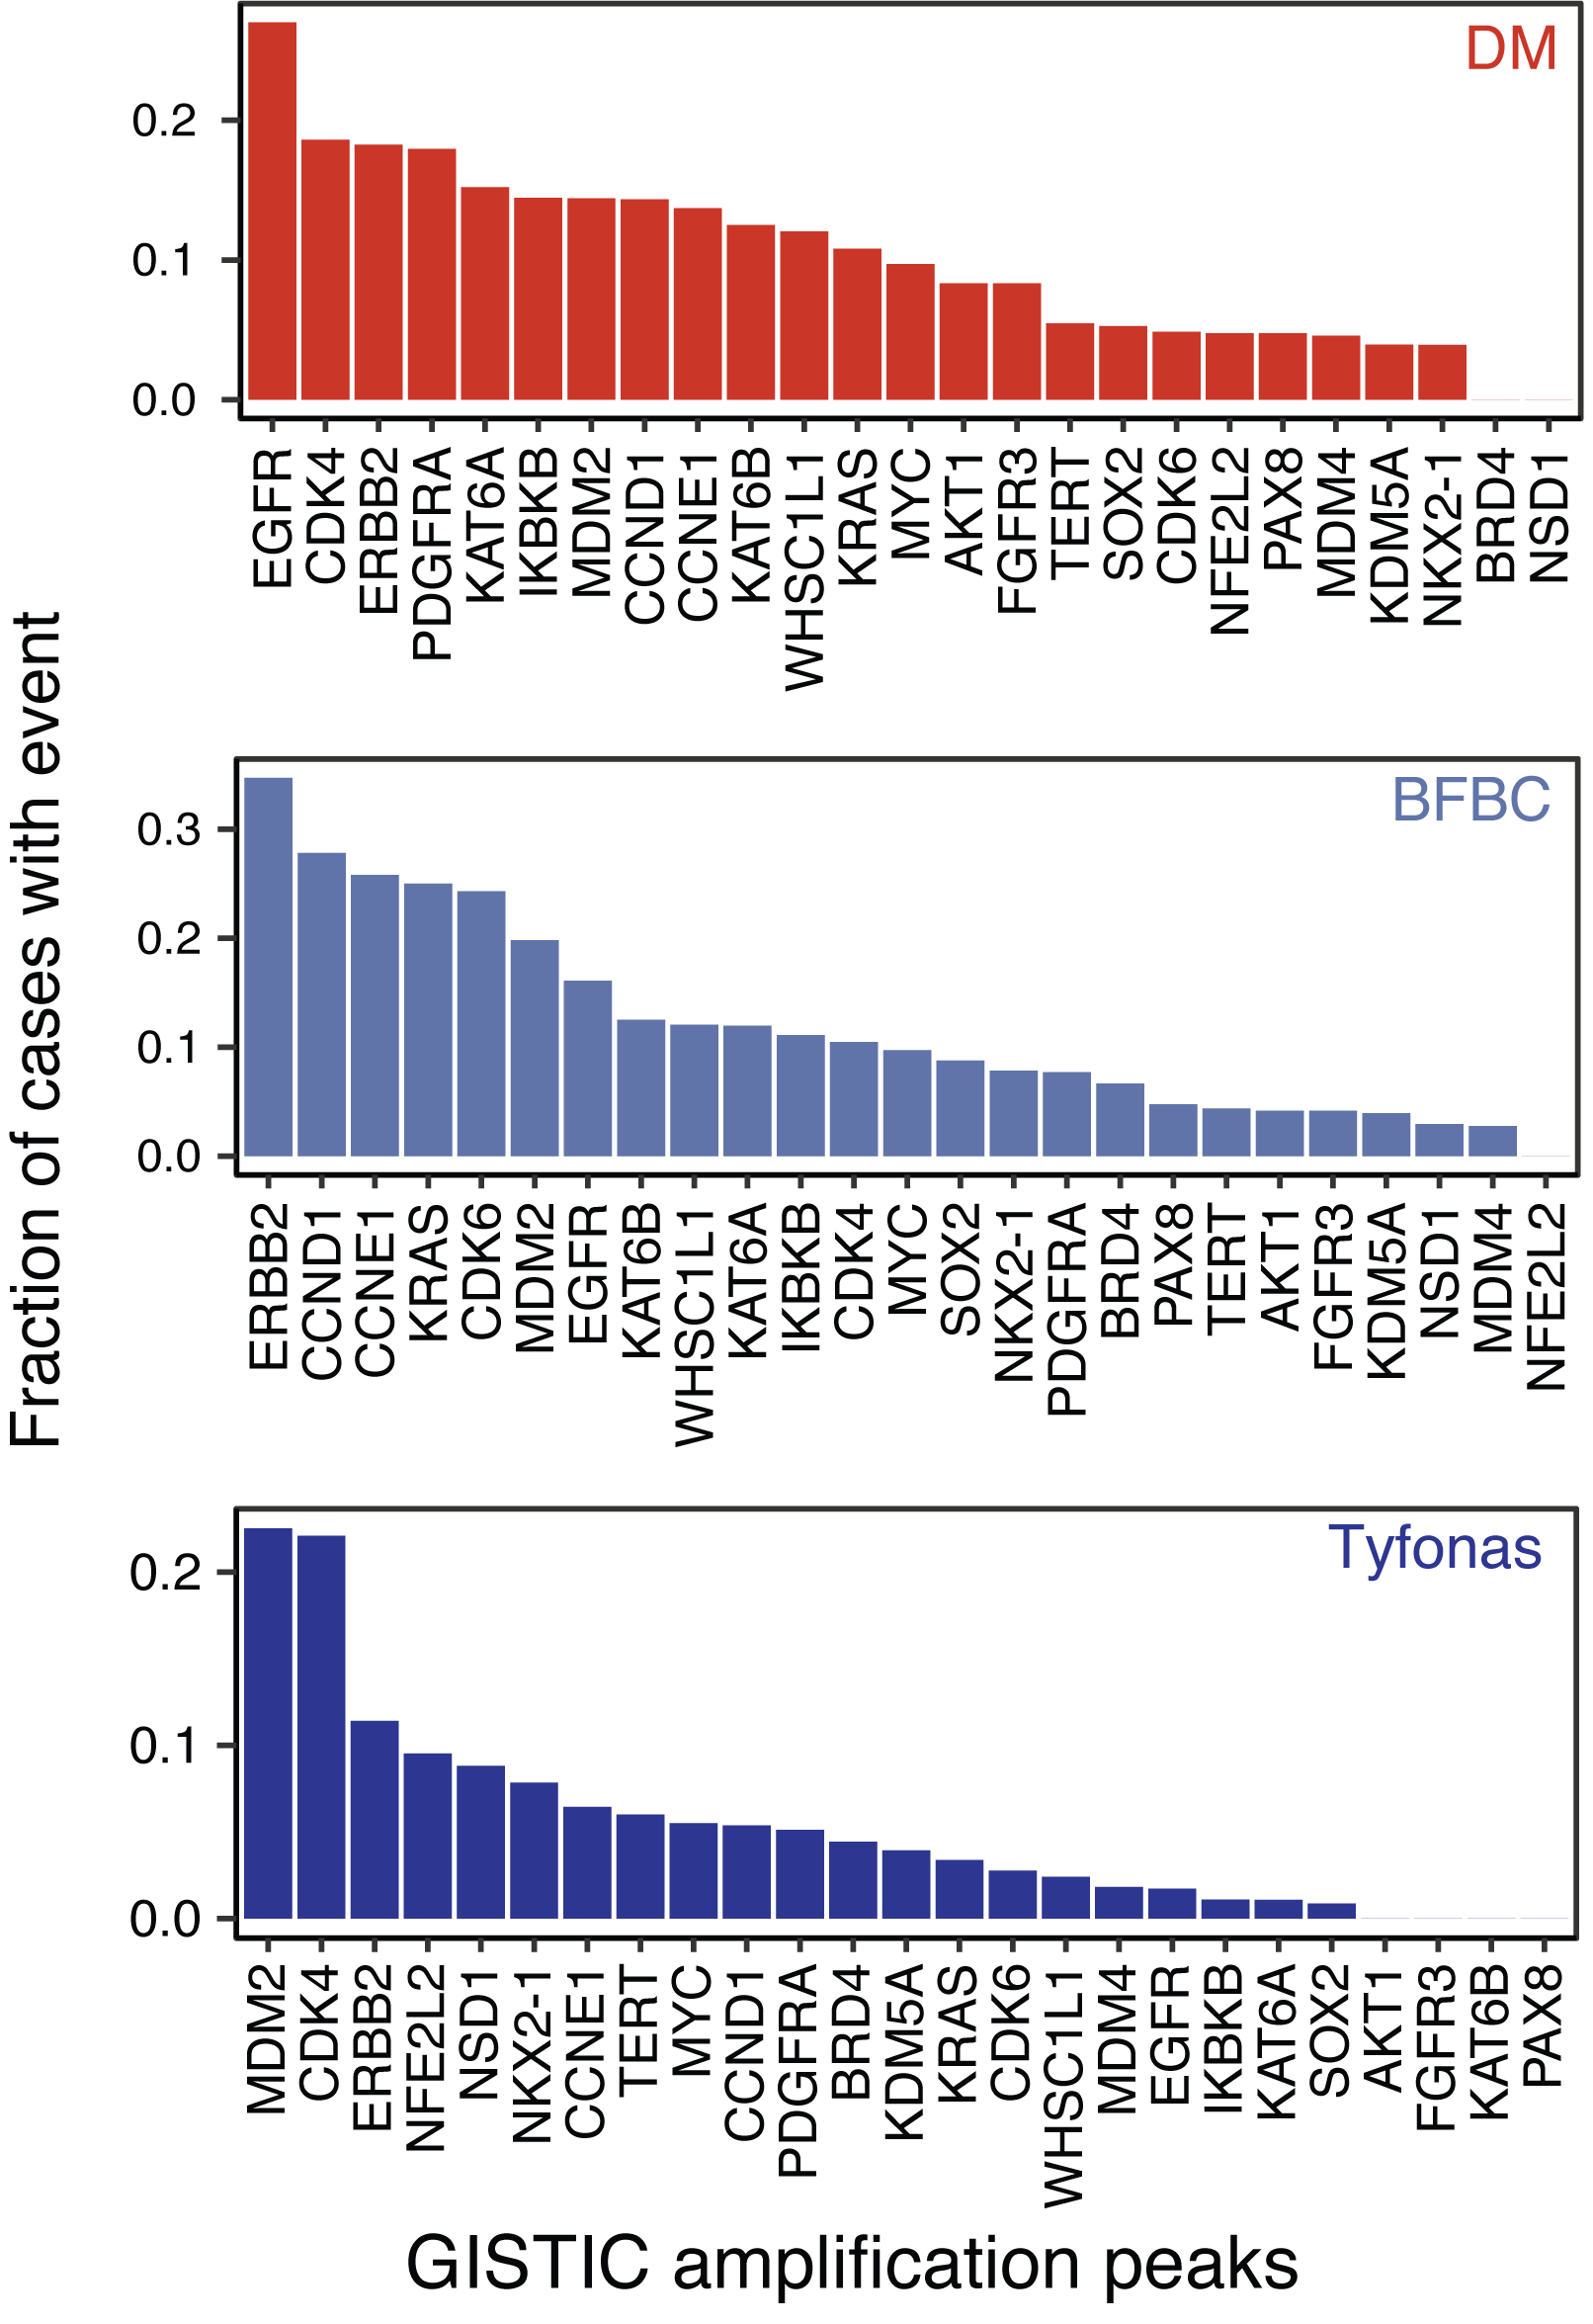
\includegraphics{figures/600ppi/amplicon_driver.png}
    \caption{\textbf{Tyfonas, DM, and BFB recurrently amplify different oncogenes}}
    \label{fig:amplicon_driver}
\end{figure}

\begin{figure}
    \centering
    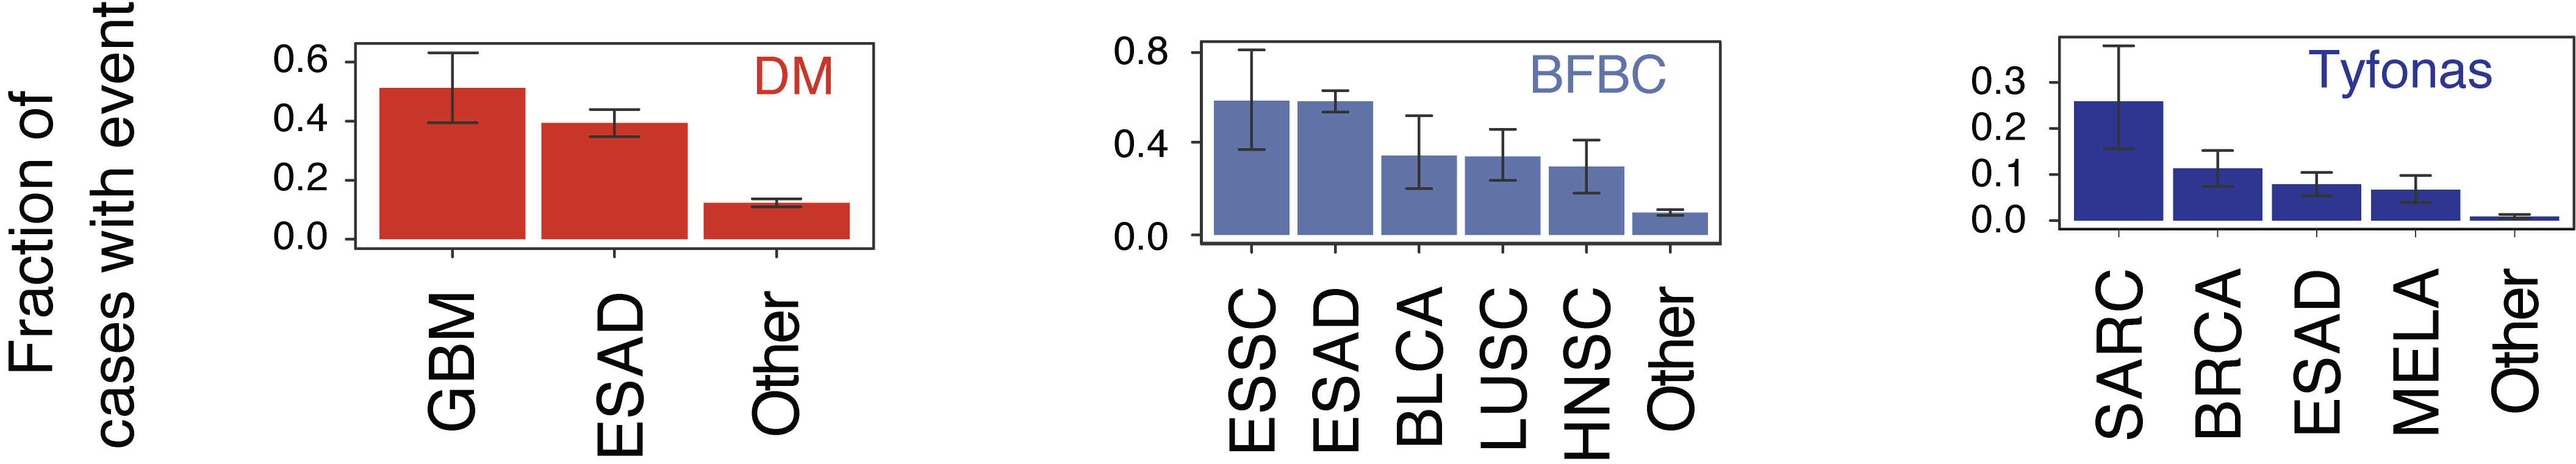
\includegraphics{figures/600ppi/amps_ttype.png}
    \caption{\textbf{Tyfonas, DM, and BFB enrich in different tumor types.}}
    \label{fig:amplicon_ttype}
\end{figure}

\begin{figure*}
    \centering
    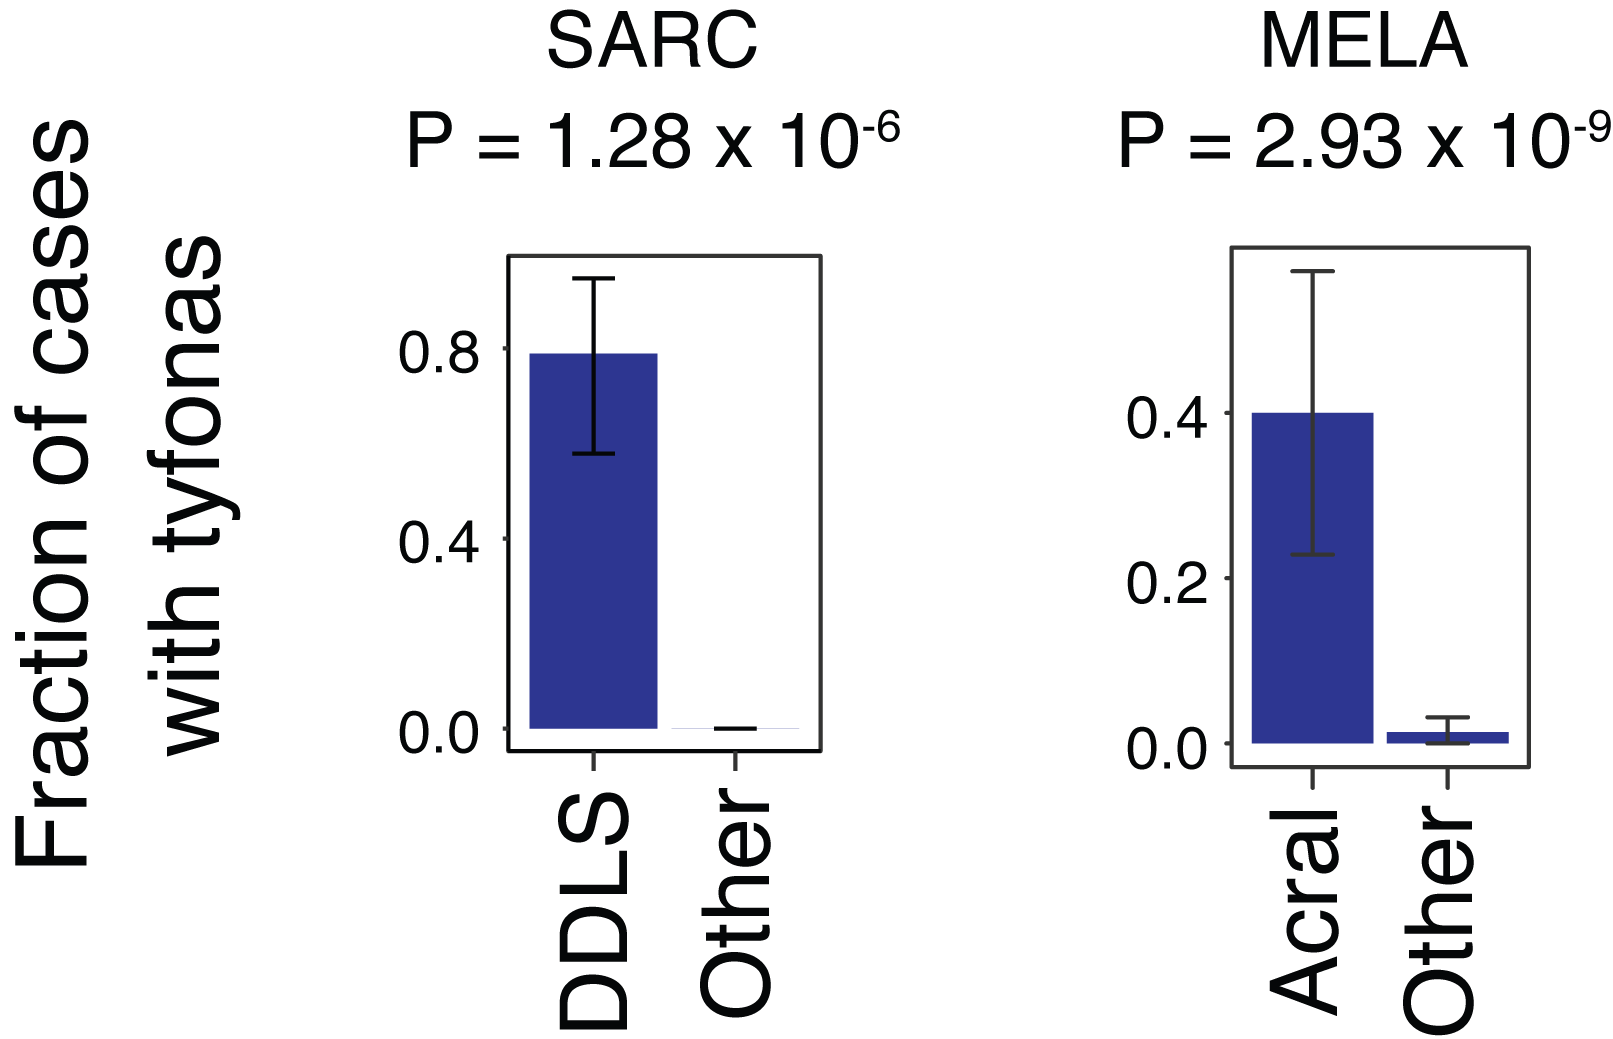
\includegraphics[width=0.95\linewidth]{figures/600ppi/tyf_ttype.png}
    \label{fig:tyf_ttype}
    \caption{\textbf{Tyfonas is highly enriched in liposarcoma and acral melanoma.}}
\end{figure*}

\begin{figure*}
    \centering
    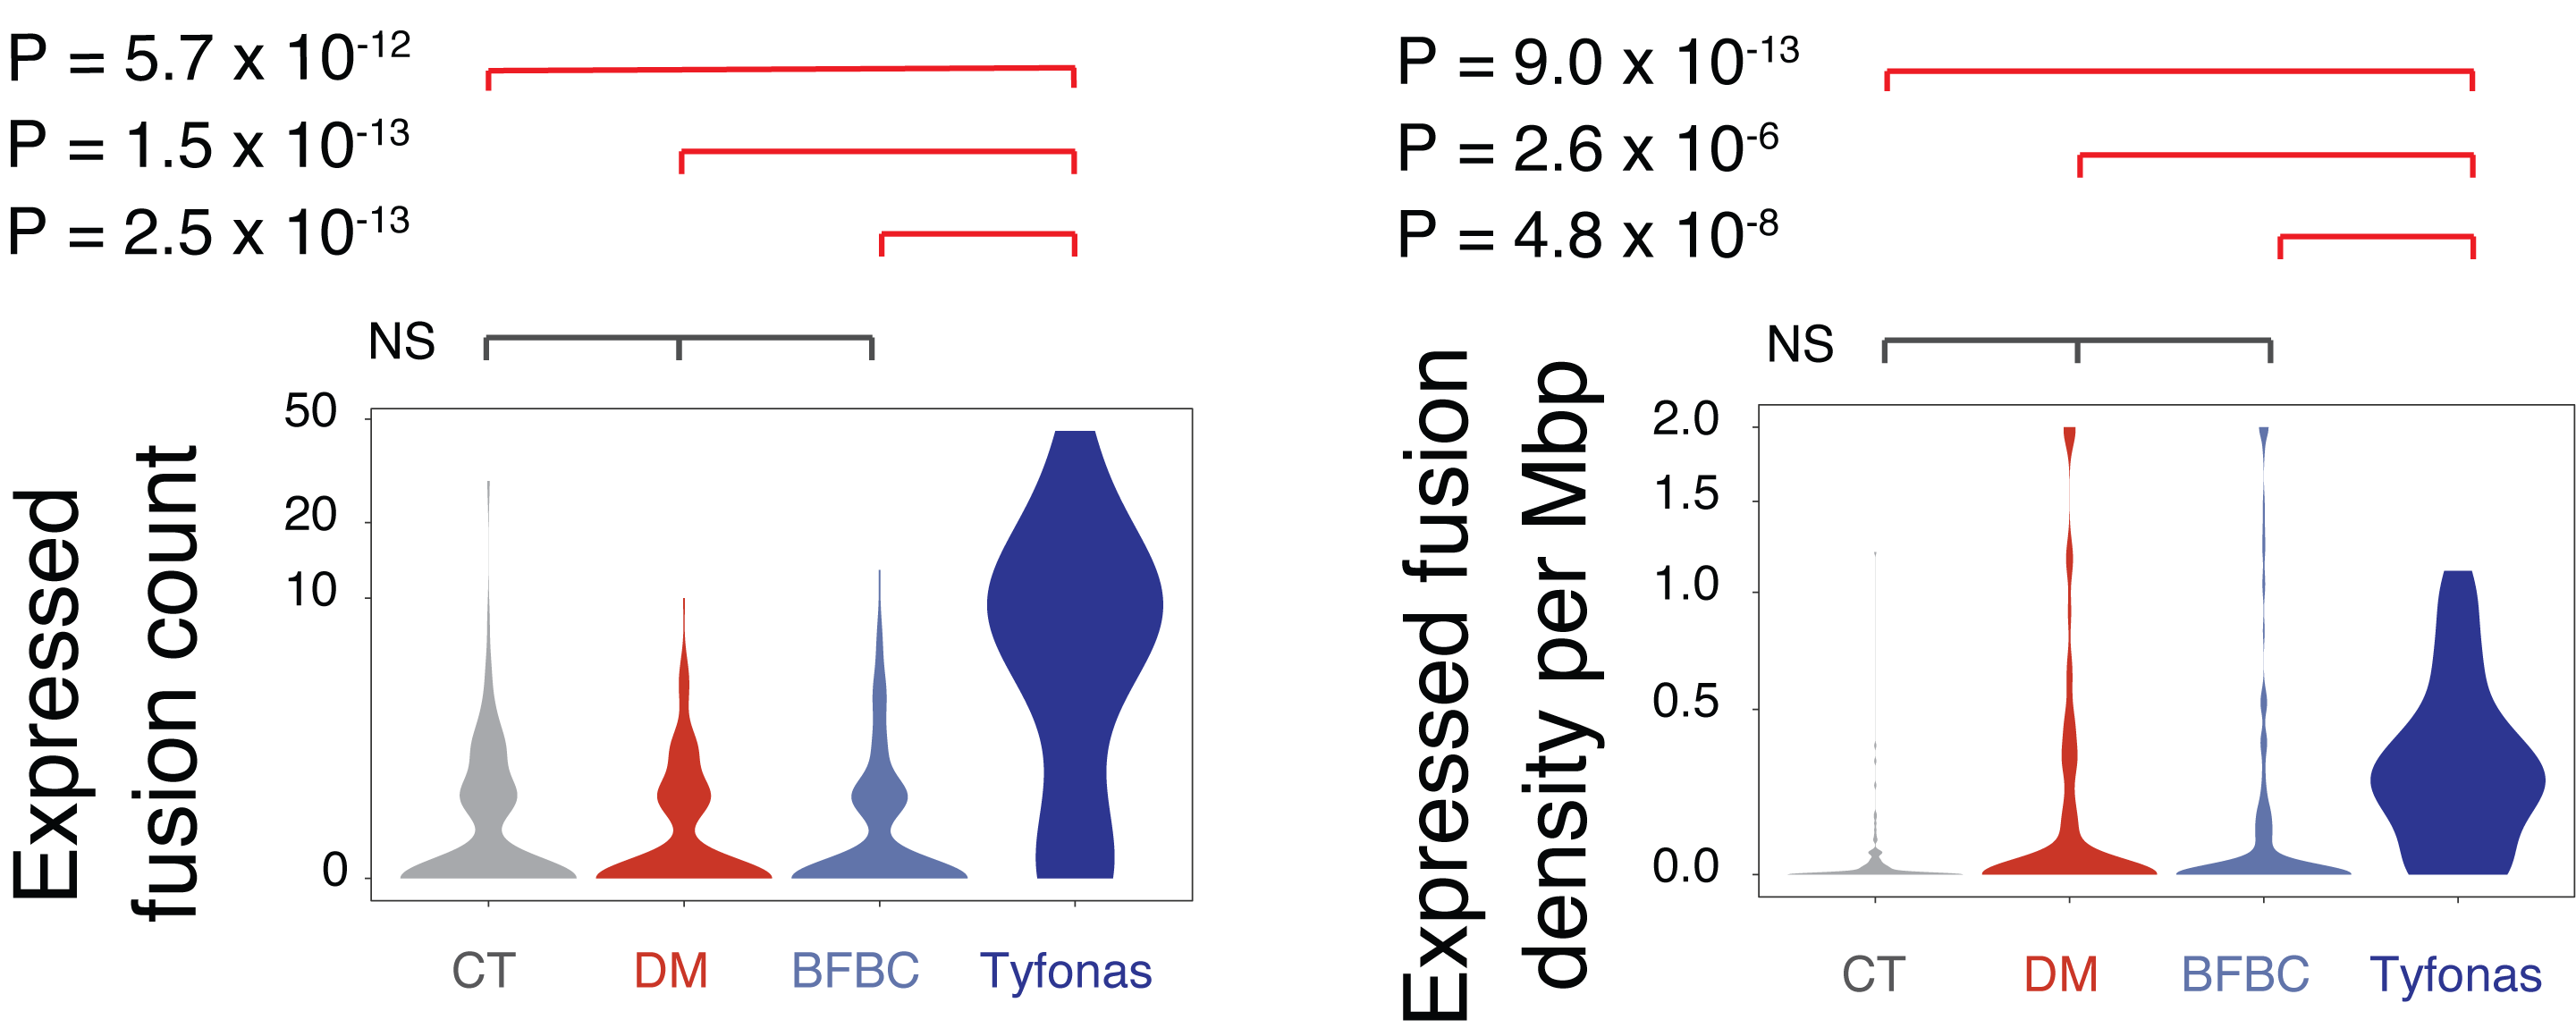
\includegraphics[width=0.95\linewidth]{figures/600ppi/tyf_fusion.png}
    \label{fig:tyf_fusion}
    \caption{\textbf{Tyfonas create more fusion genes and highly expressed fusion genes than BFB, DM, and chromothripsis.}}
\end{figure*}



% TODO: fix the table insertion
% \begin{table}[!ht]
%     \captionsetup{justification=raggedright,singlelinecheck=off}
%     \caption{\textbf{Pan-cancer WGS cohort summary, related to Figure \ref{fig:Fig1}} Summary (table in pdf format) of the number of samples from each tumor type and the number of cell line samples of a tumor type.}
%     \label{tab:S1}
% \end{table}

% \begin{table}[!ht]
%     \captionsetup{justification=raggedright,singlelinecheck=off}
%     \caption{\textbf{Sources of pan-cancer WGS datasets used in \cite{Hadi2020-um}, related to Figure \ref{fig:Fig1}} Summary (table in pdf format) of the number of samples from each dataset, the completeness of the pipelines, and the citation if the dataset is published before.}
%     \label{tab:S2}
% \end{table}

%Consistent with our 10X Chromium WGS benchmarks (see above) (\textbf{Fig. \ref{fig:Fig1}C}), we observed wide variation in inferred JCN across our datasets which correlated with observed read depth changes at breakends (\textbf{Fig. \ref{fig:Fig1}F}). 

% \section{Low JCN clusters of deletion-like and duplication-like junctions form rigma and pyrgo}
% To distinguish between complex SV patterns associated with low-JCN vs. high-JCN junctions, we identified junction clusters based on their overlapping footprints on the reference and labeled each cluster as high- / low- JCN on the basis of its highest copy junction (high-JCN thresholded at $>$ 7). Considering clusters harboring three or more junctions, we found low-JCN clusters were significantly more likely to be dominated ($>$ 90\% representation of that type) by DEL-like ($P < \SI{2.2e-16}{}$, z-test, logistic regression) or DUP-like junctions ($P < \SI{2.2e-16}{}$) (\textbf{Fig. \ref{fig:S2}A}).

% To rigorously nominate clusters of low copy DUP-like and DEL-like junctions within each tumor sample, we identified genomic tiles (1 Mbp width, 500 kbp stride) enriched in low-JCN of a given type (e.g. DEL-like) relative to a calibrated gamma-Poisson background model (see \nameref{sec:methods}). In each analysis, non-outlier tiles harbored apparent simple deletions or duplications (\textbf{Fig. \ref{fig:Fig2}A-B}). In contrast, outlier bins in the DUP-like model resembled "towers" of low-JCN DUP-like junctions  (\textbf{Fig. \ref{fig:Fig2}A, top right}) that we named \textit{pyrgo} (\textgreek{p'urgos}, Greek meaning tower). Outlier loci in the DEL-like models comprised subgraphs of interval CN "chasms" flanked by low-JCN DEL-like junctions whose interval CN often reached 0 (\textbf{Fig. \ref{fig:Fig2}B, top left}).  We named these patterns \textit{rigma} (ρήγμα, Greek meaning rift).

\section{Tyfonas is massively rearranged amplicon associated with elevated number of fusion genes}
We then sought to investigate the rearrangement patterns associated with high-JCN junctions (JCN $>$ 7) in our genome graphs.  \textit{A priori}, a junction at such an extreme of JCN may evolve through a double minute, BFBC, or an as yet undescribed mechanism for duplicating already rearranged DNA. To characterize classes of  amplification events associated with these high-JCN junctions, we first identified 12,588 subgraphs harboring an interval CN of at least twice ploidy among the 2,487 unique genome graphs (by patient) (Figure \ref{fig:amplicon_features}), then identified among these amplicons (amplified clusters within a genome) those that harbor at least one junction with JCN $>$ 7.  We annotated the resulting 1,703 high-JCN amplicons according to three features: 1) the maximum JCN normalized by the maximal interval CN, 2) the \textit{sum} of fold back inversion JCNs (INV-like junctions that terminate and begin at nearly the same location in the genome) relative to the maximal interval CN, and 3) the number of junctions with elevated JCN (JCN>3) (see \nameref{app:a}).

Clustering and classification of amplicons (Figure \ref{fig:amplicon_definition}) on the basis of these three features yielded three stable clusters (Figure \ref{fig:amplicon_definition},\ref{fig:amplicon_jaccard},\ref{fig:amplicon_pca}; see also \nameref{app:b}).  Upon visual inspection, the first group, harboring low fold-back JCN but high maximal JCN, contained amplicons comprising a single high-JCN junction forming a high CN circular path in the graph (Figure \ref{fig:dm_example}) as well as more complex cyclic patterns spanning multiple discontiguous loci, consistent with a double minute (or extrachromosomal circular DNAs).  The second group, demonstrating high fold-back JCN ($>$ 0.5), a low burden of elevated-JCN junctions ($<$ 26), and a "stair step" pattern of copy gains, was consistent with a BFBC (Figure \ref{fig:bfb_example}, \cite{Zakov:2013cm,McClintock1939-oi}). The third group contained both high fold-back JCN ($\geq$0.50) and a significant burden of elevated JCN junctions ($\geq$26).  Upon visual inspection, these amplicons comprised dense webs of elevated  JCN junctions across subgraphs compris $>$ 100 Mbp of genomic material and often reaching CNs higher than 50 (Figure \ref{fig:tyf_example}).  We dubbed these extremely large amplicons, which did not fit in previously defined categories, \textit{tyfonas} (τύφωνας, Greek meaning typhoon) (Figure \ref{fig:tyf_example}).

\subsection*{Tyfonas are distinct from BFBCs and double minutes}
Comparing amplicon features, we found that tyfonas had significantly larger genomic mass (summed interval width weighted by CN, Figure \ref{fig:amplicon_mass}), maximum interval CN (Figure \ref{fig:amplicon_cn}), junction burden (Figure \ref{fig:amplicon_njunc}), and JCN entropy (based on the distribution of JCN in the amplicon, the higher the more diversity among the JCNs, Figure \ref{fig:amplicon_jcn_entropy}) than either double minutes or BFBCs ($P$ < \SI{2.2e-16}, Wilcoxon rank-sum test).  All three amplicon classes frequently intersected CGC cancer genes residing within GISTIC pan-cancer amplification peaks (Figure \ref{fig:amplicon_driver}, recurrent amplification peaks from \cite{Zack:2013f1f}). \textit{EGFR} was the most frequent target of double minutes.  BFBCs were most frequently implicated in \textit{ERBB2}, \textit{CCND1}, and \textit{CCNE1} amplification. Tyfonas were associated with \textit{MDM2} and \textit{CDK4}. While double minutes were enriched in glioblastoma and small cell lung cancer, BFBCs were enriched in esophageal squamous cell cancer, lung squamous cell cancer, and head and neck squamous cell cancer (FDR $<$ 0.25, Fisher's exact test, \textbf{Fig. \ref{fig:Figure4}F}). In contrast, tyfonas events were enriched in sarcoma, breast cancer, and melanoma (FDR $<$ 0.25).

% The specificity of tyfonas for these tumor types was much higher than for liposarcoma-like or amplified chromothripsis, which are recently proposed PCAWG categories that also showed substantial overlap with BFBC and double minutes (\textbf{Fig. \ref{fig:S4}E-K}) \cite{pcawg_marker2020-yi}.

Analyzing tumor subtypes, we found tyfonas were common in dedifferentiated liposarcomas (80\%) and acral melanomas (40\%) but rarely seen ($<$ 2\%) in fibrosarcomas and cutaneous melanomas (Figure \ref{fig:tyf_ttype}).    80\% of dedifferentiated liposarcomas harbored a tyfonas on chromosome 12q, suggesting that tyfonas represent the genomic footprint of supernumerary ring chromosomes in this tumor type \cite{Reimann2008-tj}. Given the enrichment of tyfonas events in acral melanoma, an immunotherapy-responsive melanoma with a low SNV burden \cite{Shoushtari2016-de}, we hypothesized that tyfonas events may provide an alternate source of neoantigens through the generation of expressed protein-coding fusions.  Analyzing the subset of our samples with RNA-seq data within the TCGA dataset, we found that tyfonas were significantly enriched with expressed fusion transcripts relative to double minutes, BFBCs, and even chromothripsis (CT) (Figure \ref{fig:tyf_fusion}, left), even after accounting for the larger genomic footprint of tyfonas (Figure \ref{fig:tyf_fusion}, right).

\section{Clusters of pan-cancer patients based on SV event burdens show differential prognosis and is associated with tumor types and genetic backgrounds}
\begin{figure}
    \centering
    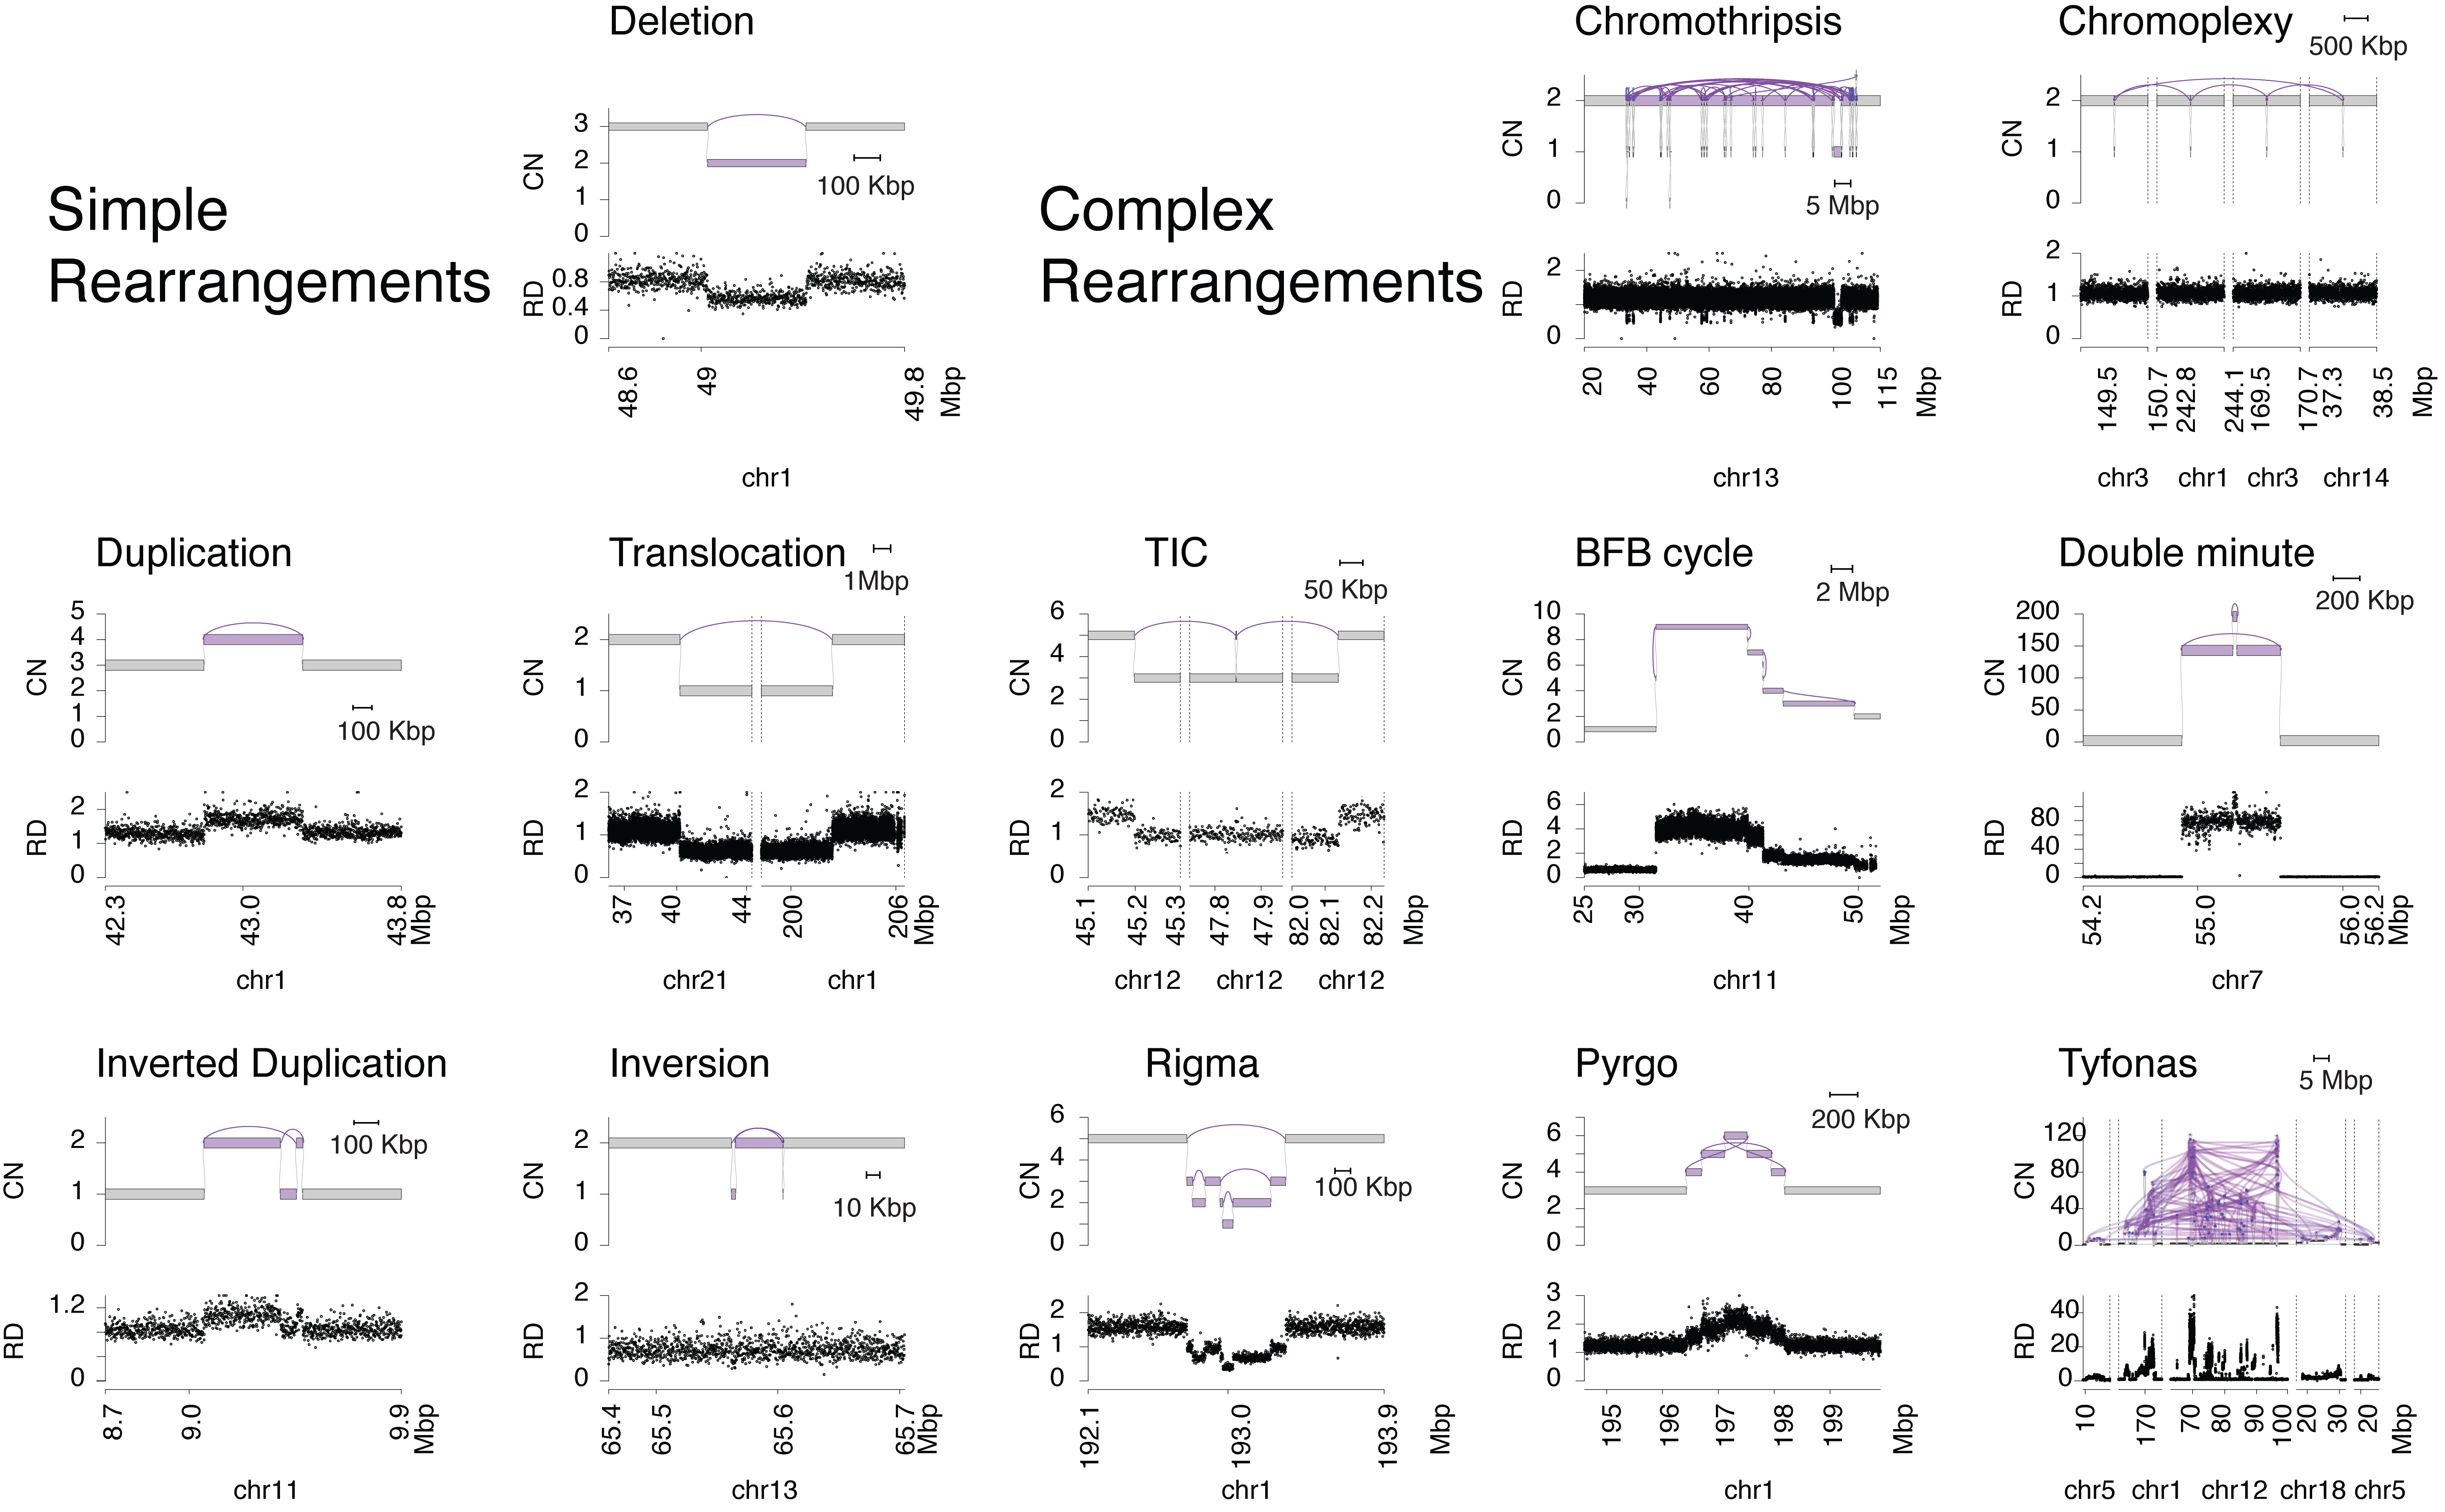
\includegraphics[width=0.95\linewidth]{figures/600ppi/sv_gallery.png}
    \caption{\textbf{Thirteen classes of simple and complex SV events defined in gGnome.}}
    \label{fig:sv_gallery}
\end{figure}

\begin{figure}
    \centering
    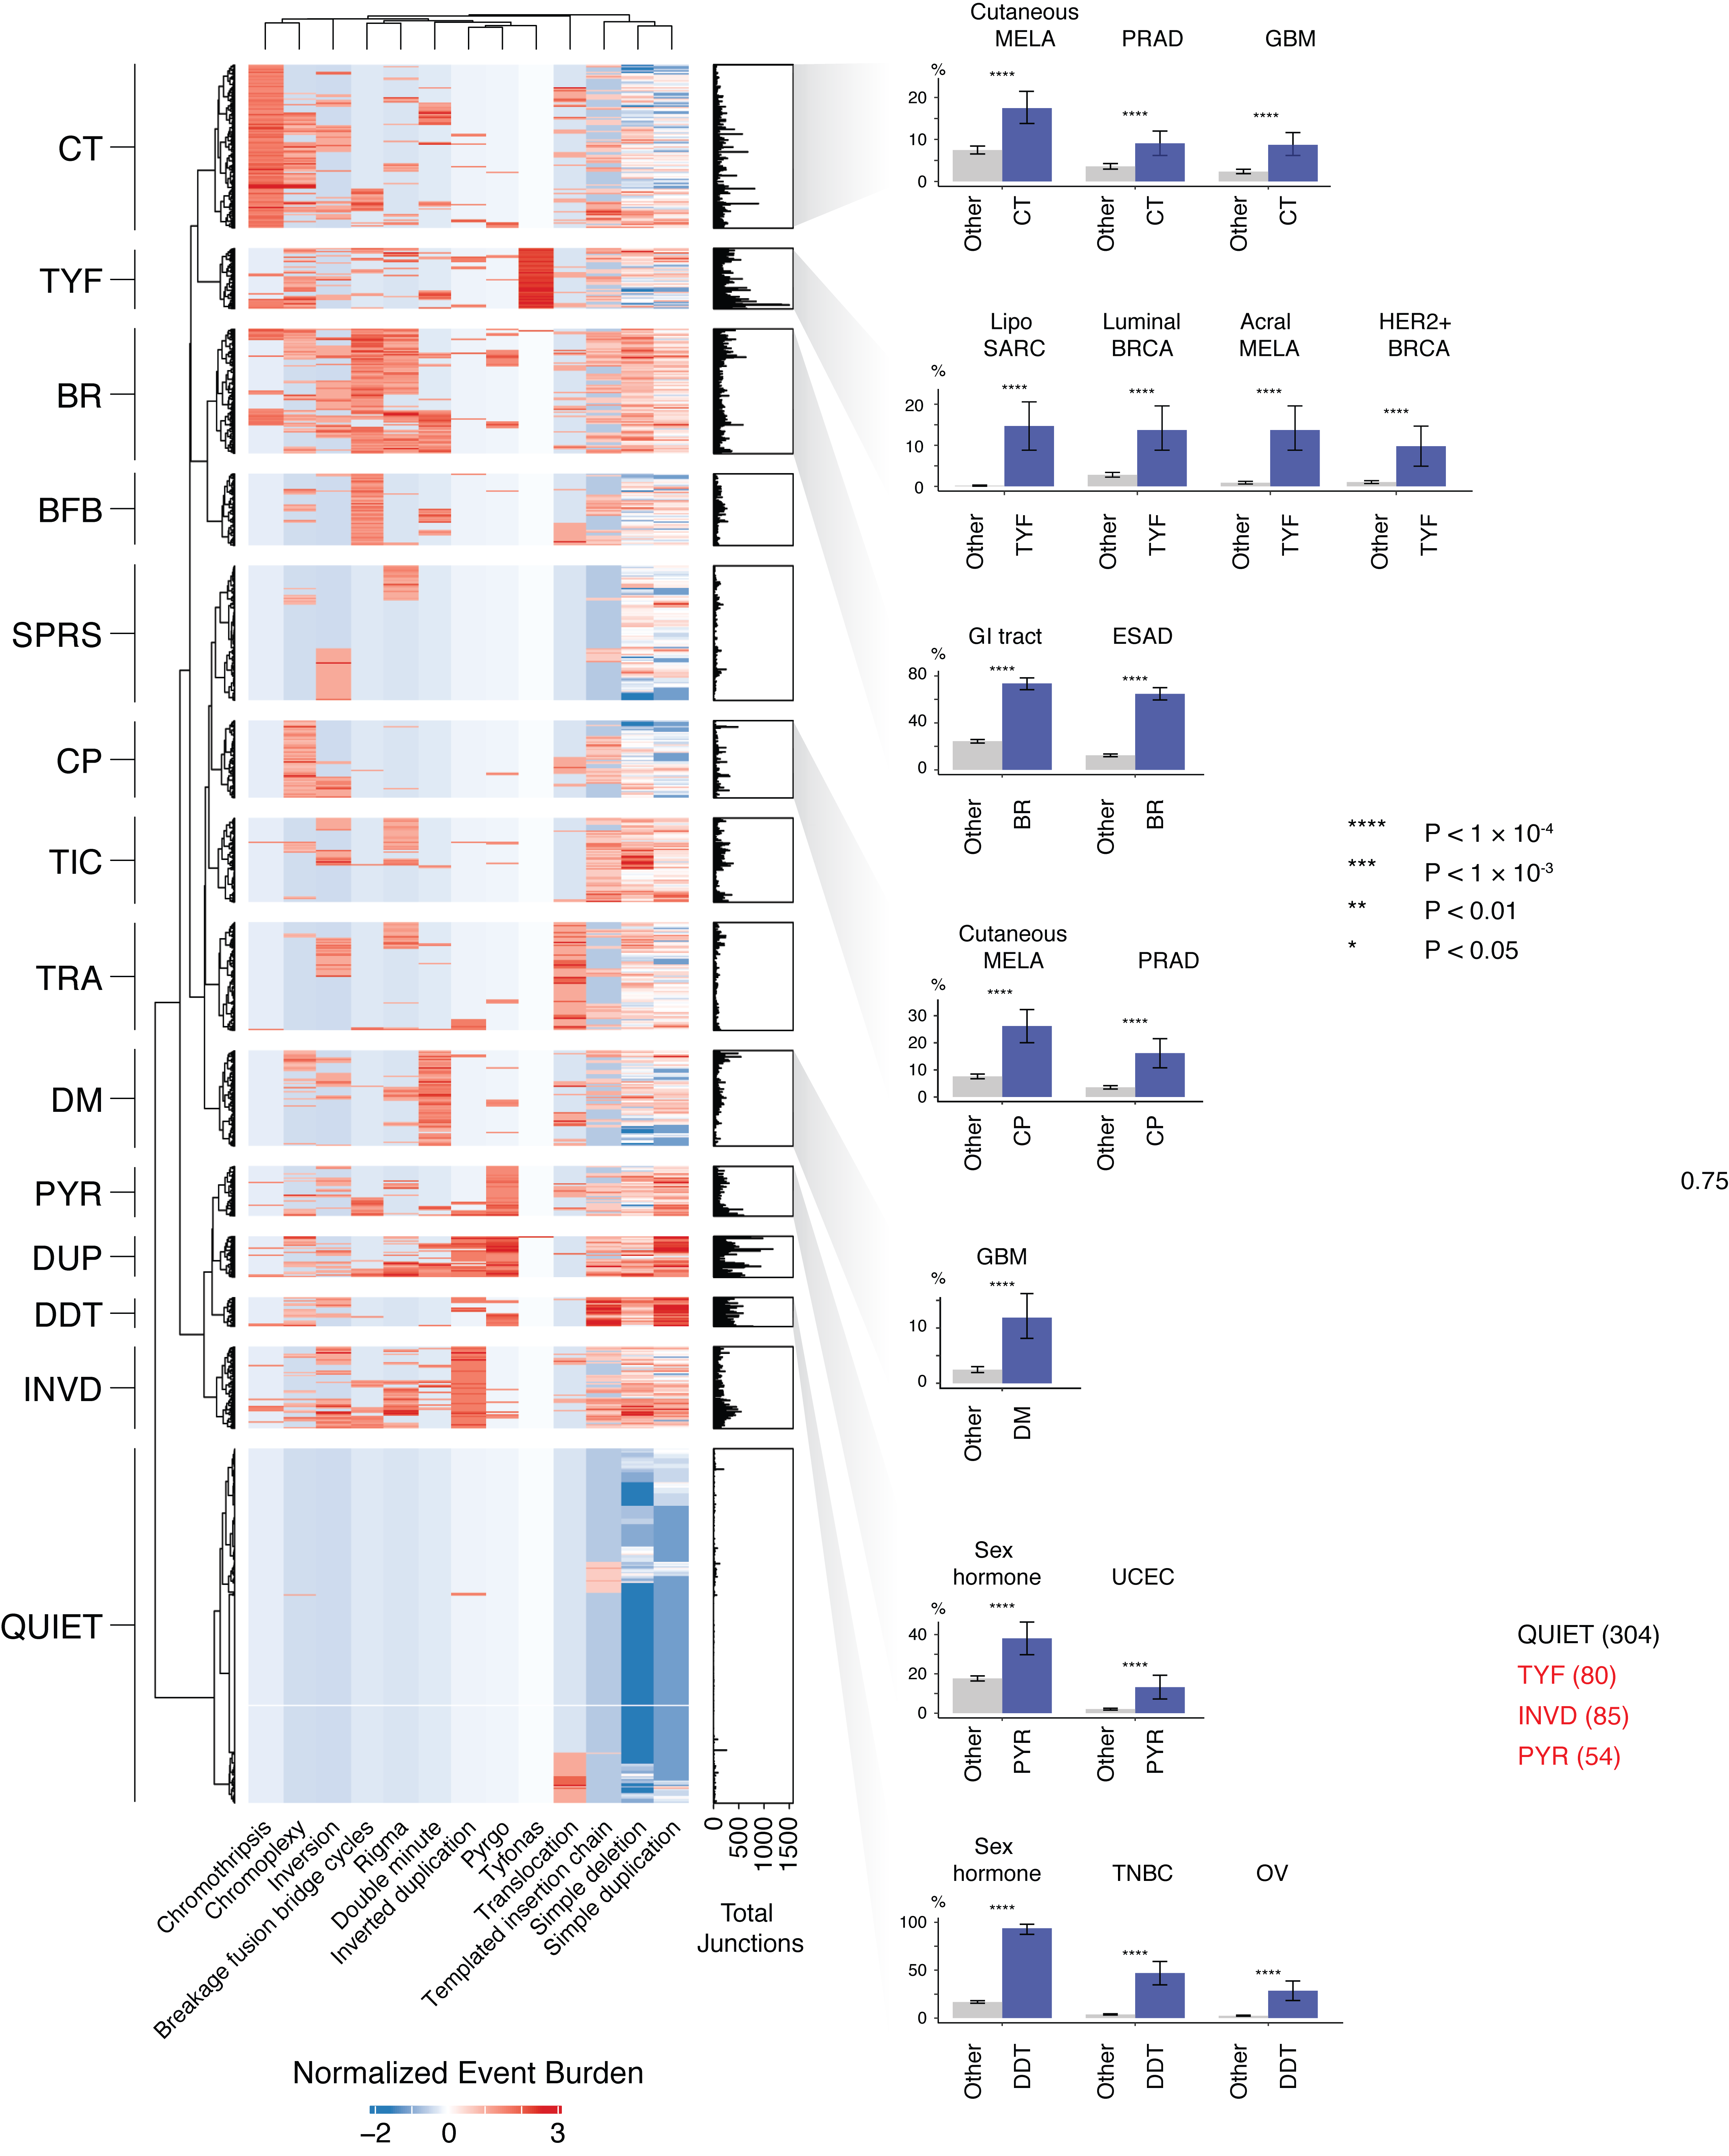
\includegraphics[width=0.95\linewidth]{figures/600ppi/clustering_heat_tt.png}
    \caption{\textbf{}}
    \label{fig:clustering_heat_tt}
\end{figure}

\begin{figure}
    \centering
    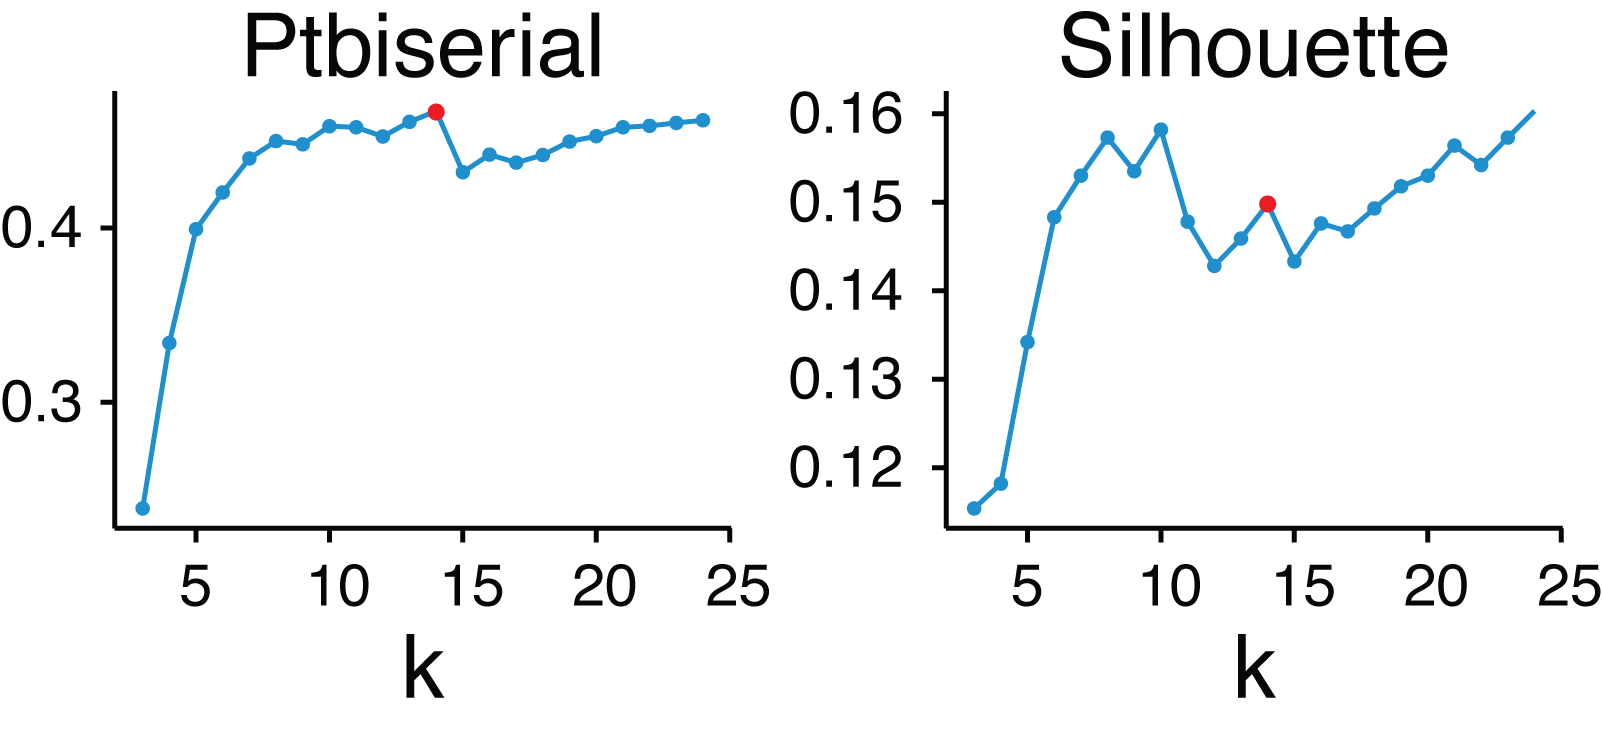
\includegraphics[width=0.95\linewidth]{figures/600ppi/clustering_find_k.png}
    \caption{\textbf{Metrics for determining the optimal number of clusters.}}
    \label{fig:find_k}
\end{figure}

\begin{figure}
    \centering
    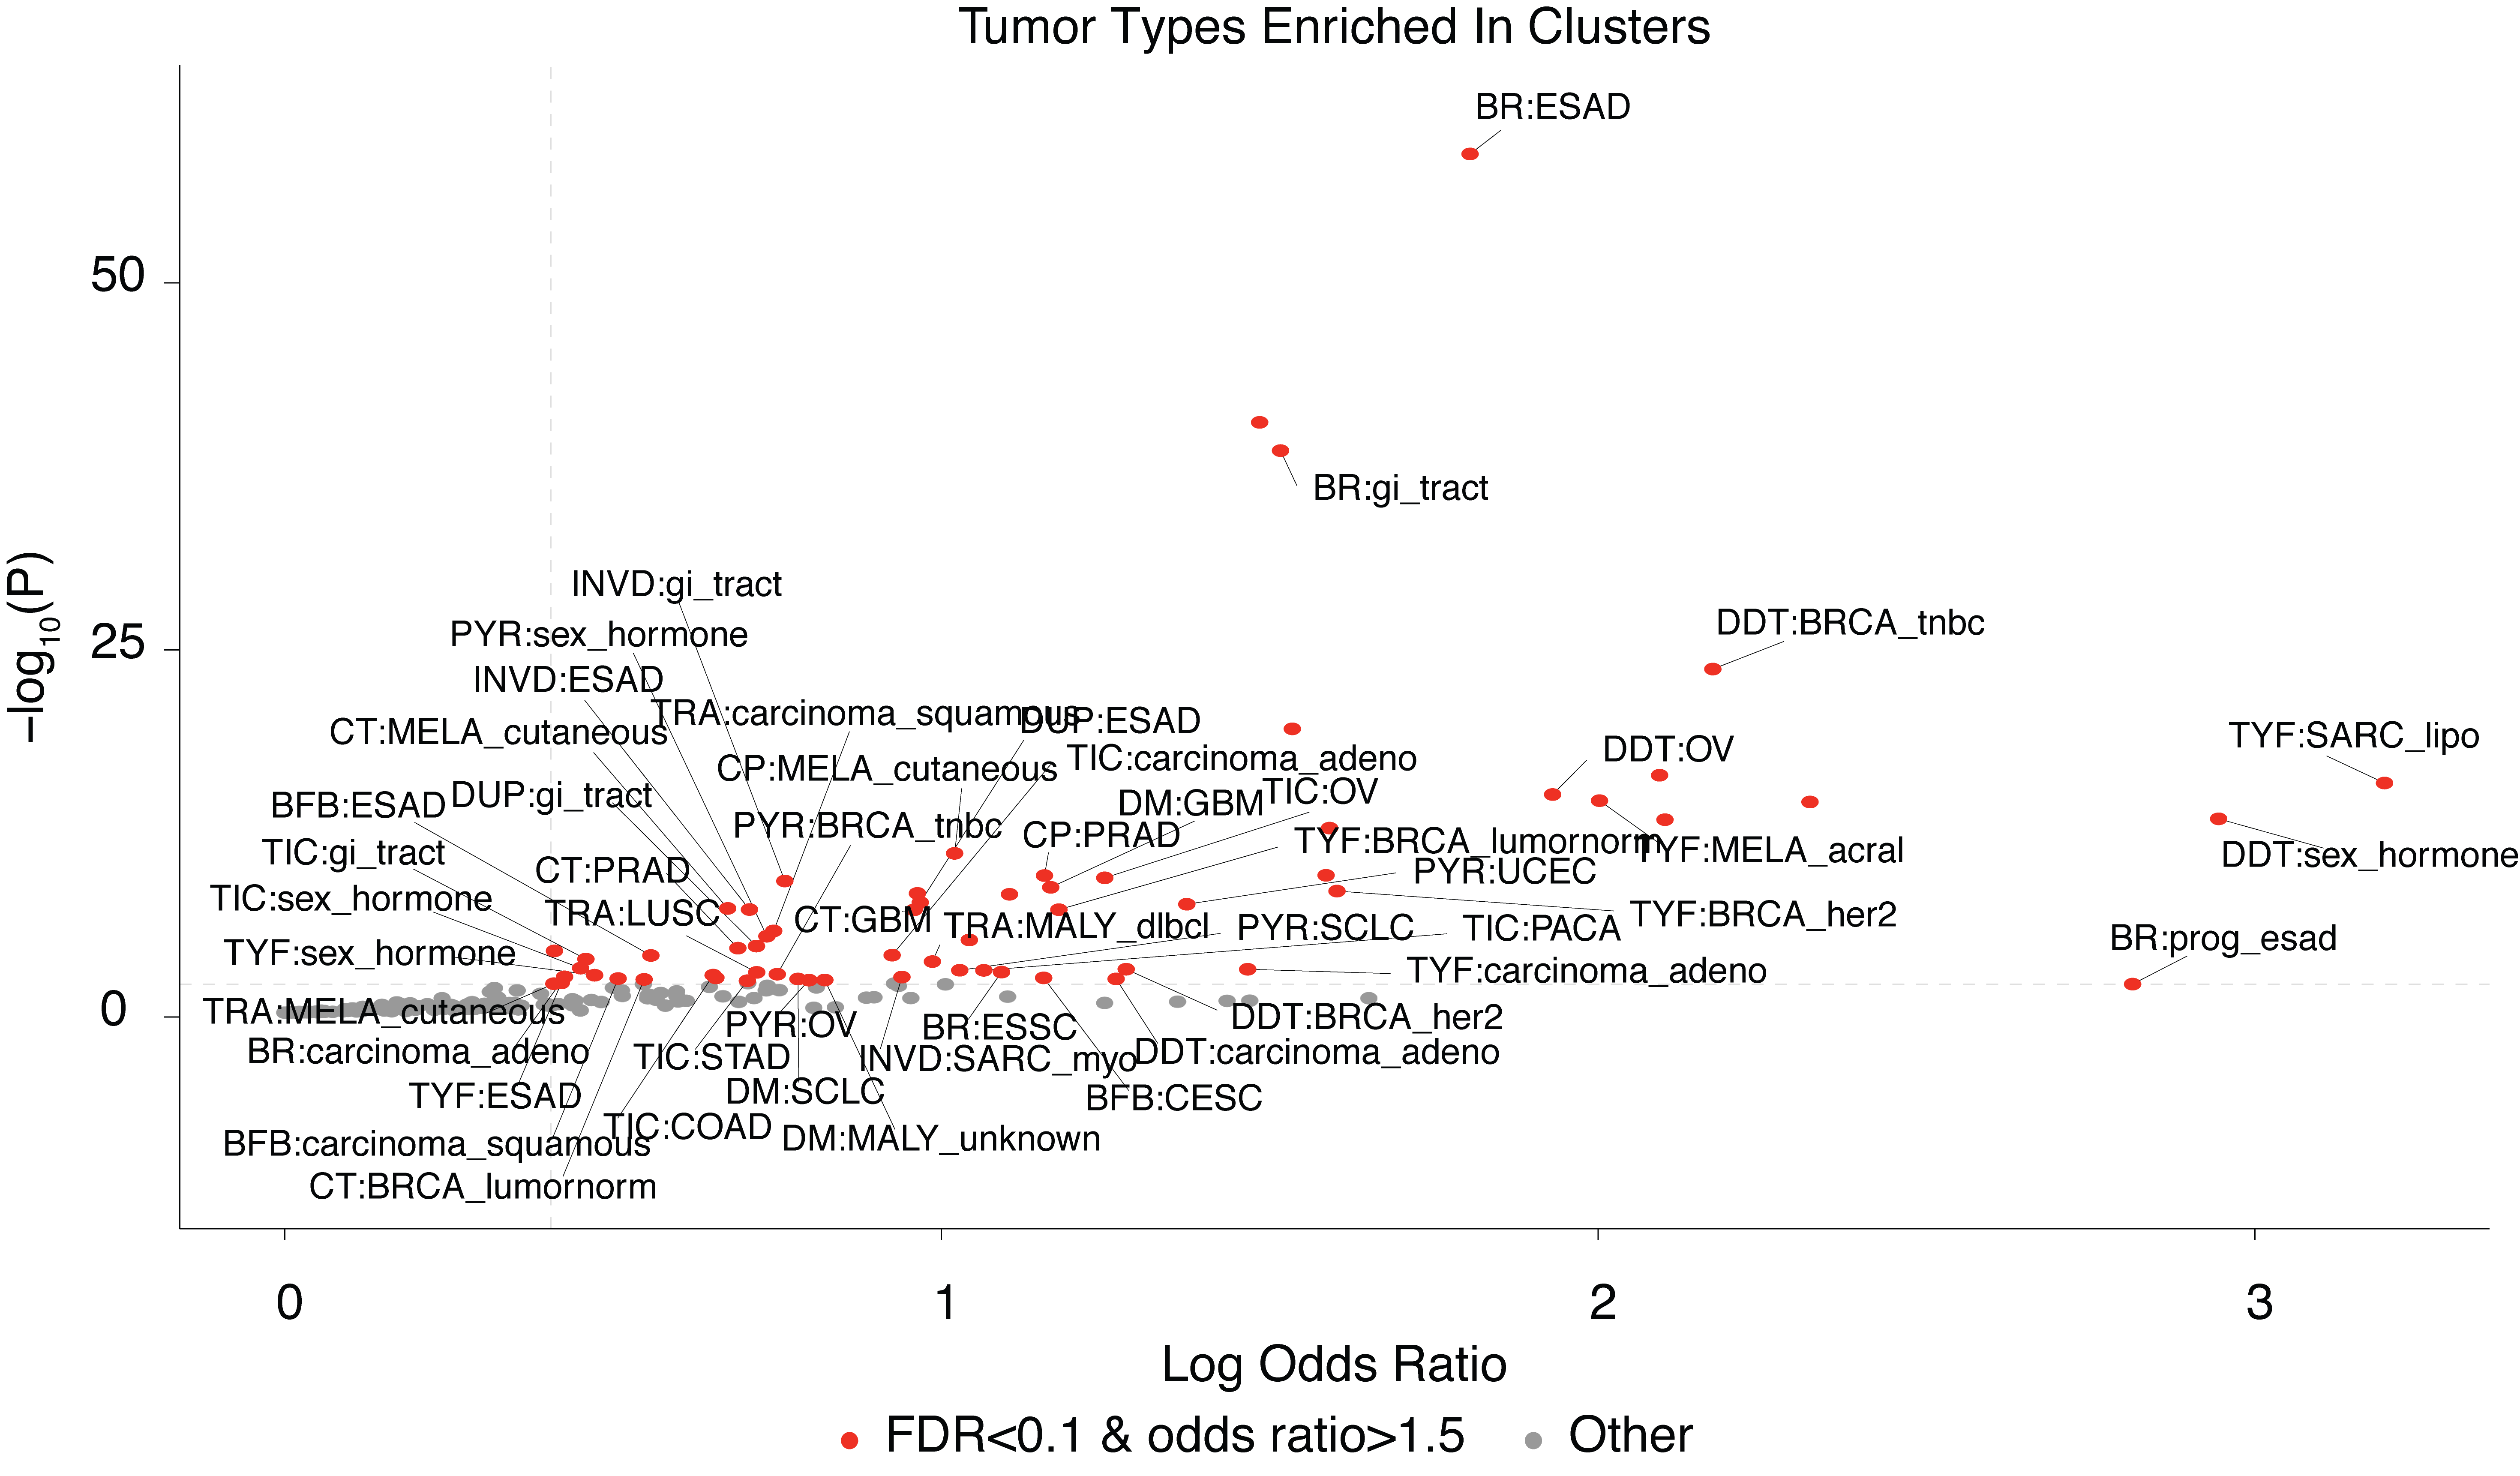
\includegraphics[width=0.95\linewidth]{figures/600ppi/clustering_tt_all.png}
    \caption{\textbf{All associations between clusters and tumor types.}}
    \label{fig:clustering_tt_all}
\end{figure}

\begin{figure}
    \centering
    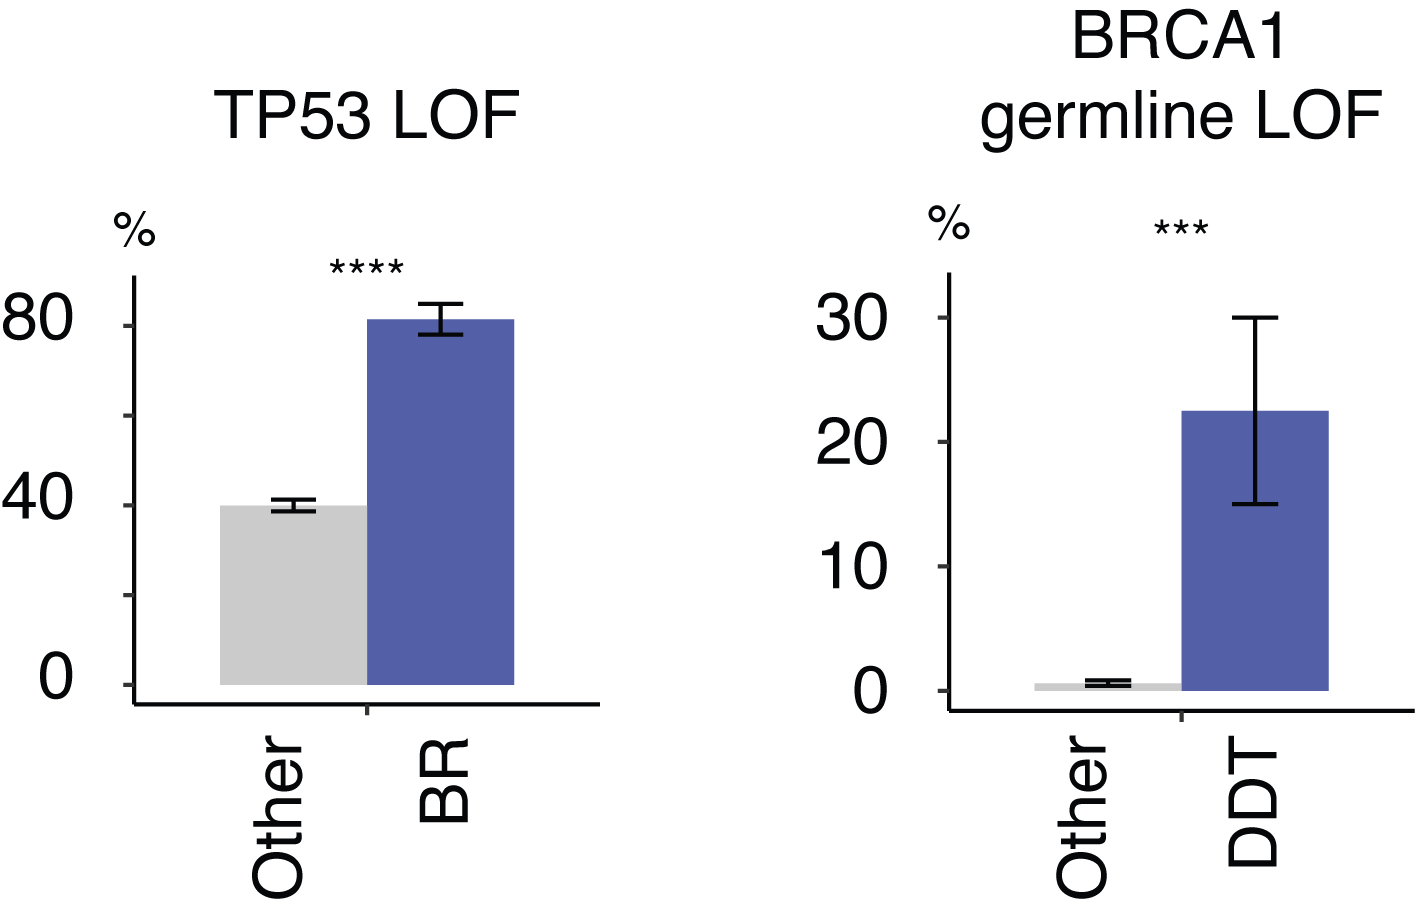
\includegraphics[width=0.95\linewidth]{figures/600ppi/clustering_geno.png}
    \caption{\textbf{DDT cluster is associated with BRCA1 familial LoF alterations and BR cluster with TP53 LoF.}}
    \label{fig:clustering_geno}
\end{figure}

\begin{figure}
    \centering
    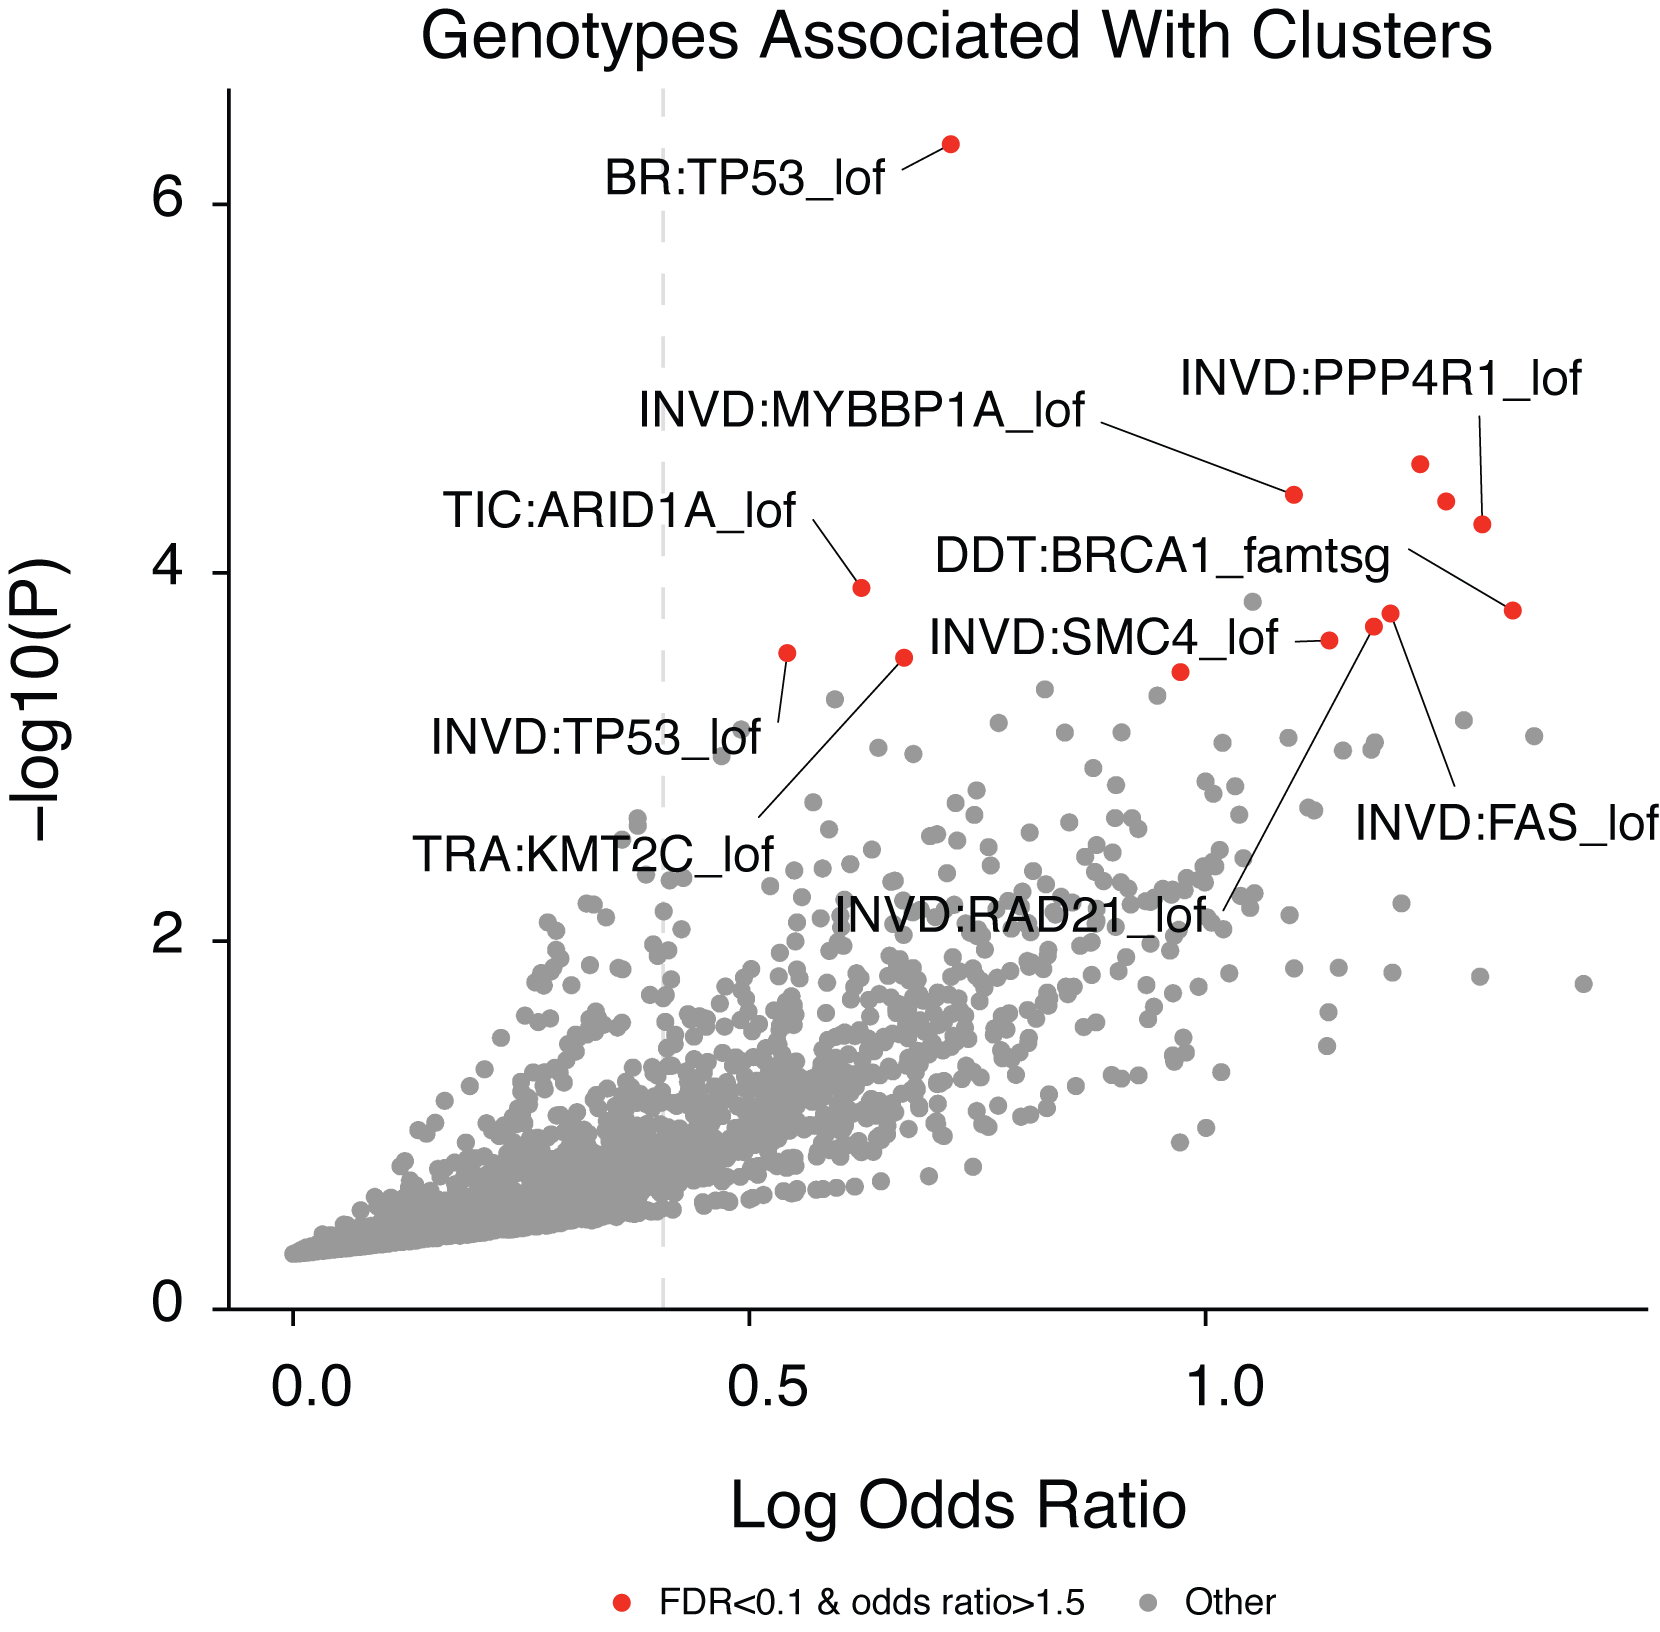
\includegraphics[width=0.95\linewidth]{figures/600ppi/clustering_geno_all.png}
    \caption{\textbf{All associations between clusters and LoF alterations of tumor suppressors or DNA damage response genes.}}
    \label{fig:clustering_geno_all}
\end{figure}

\begin{figure}
    \centering
    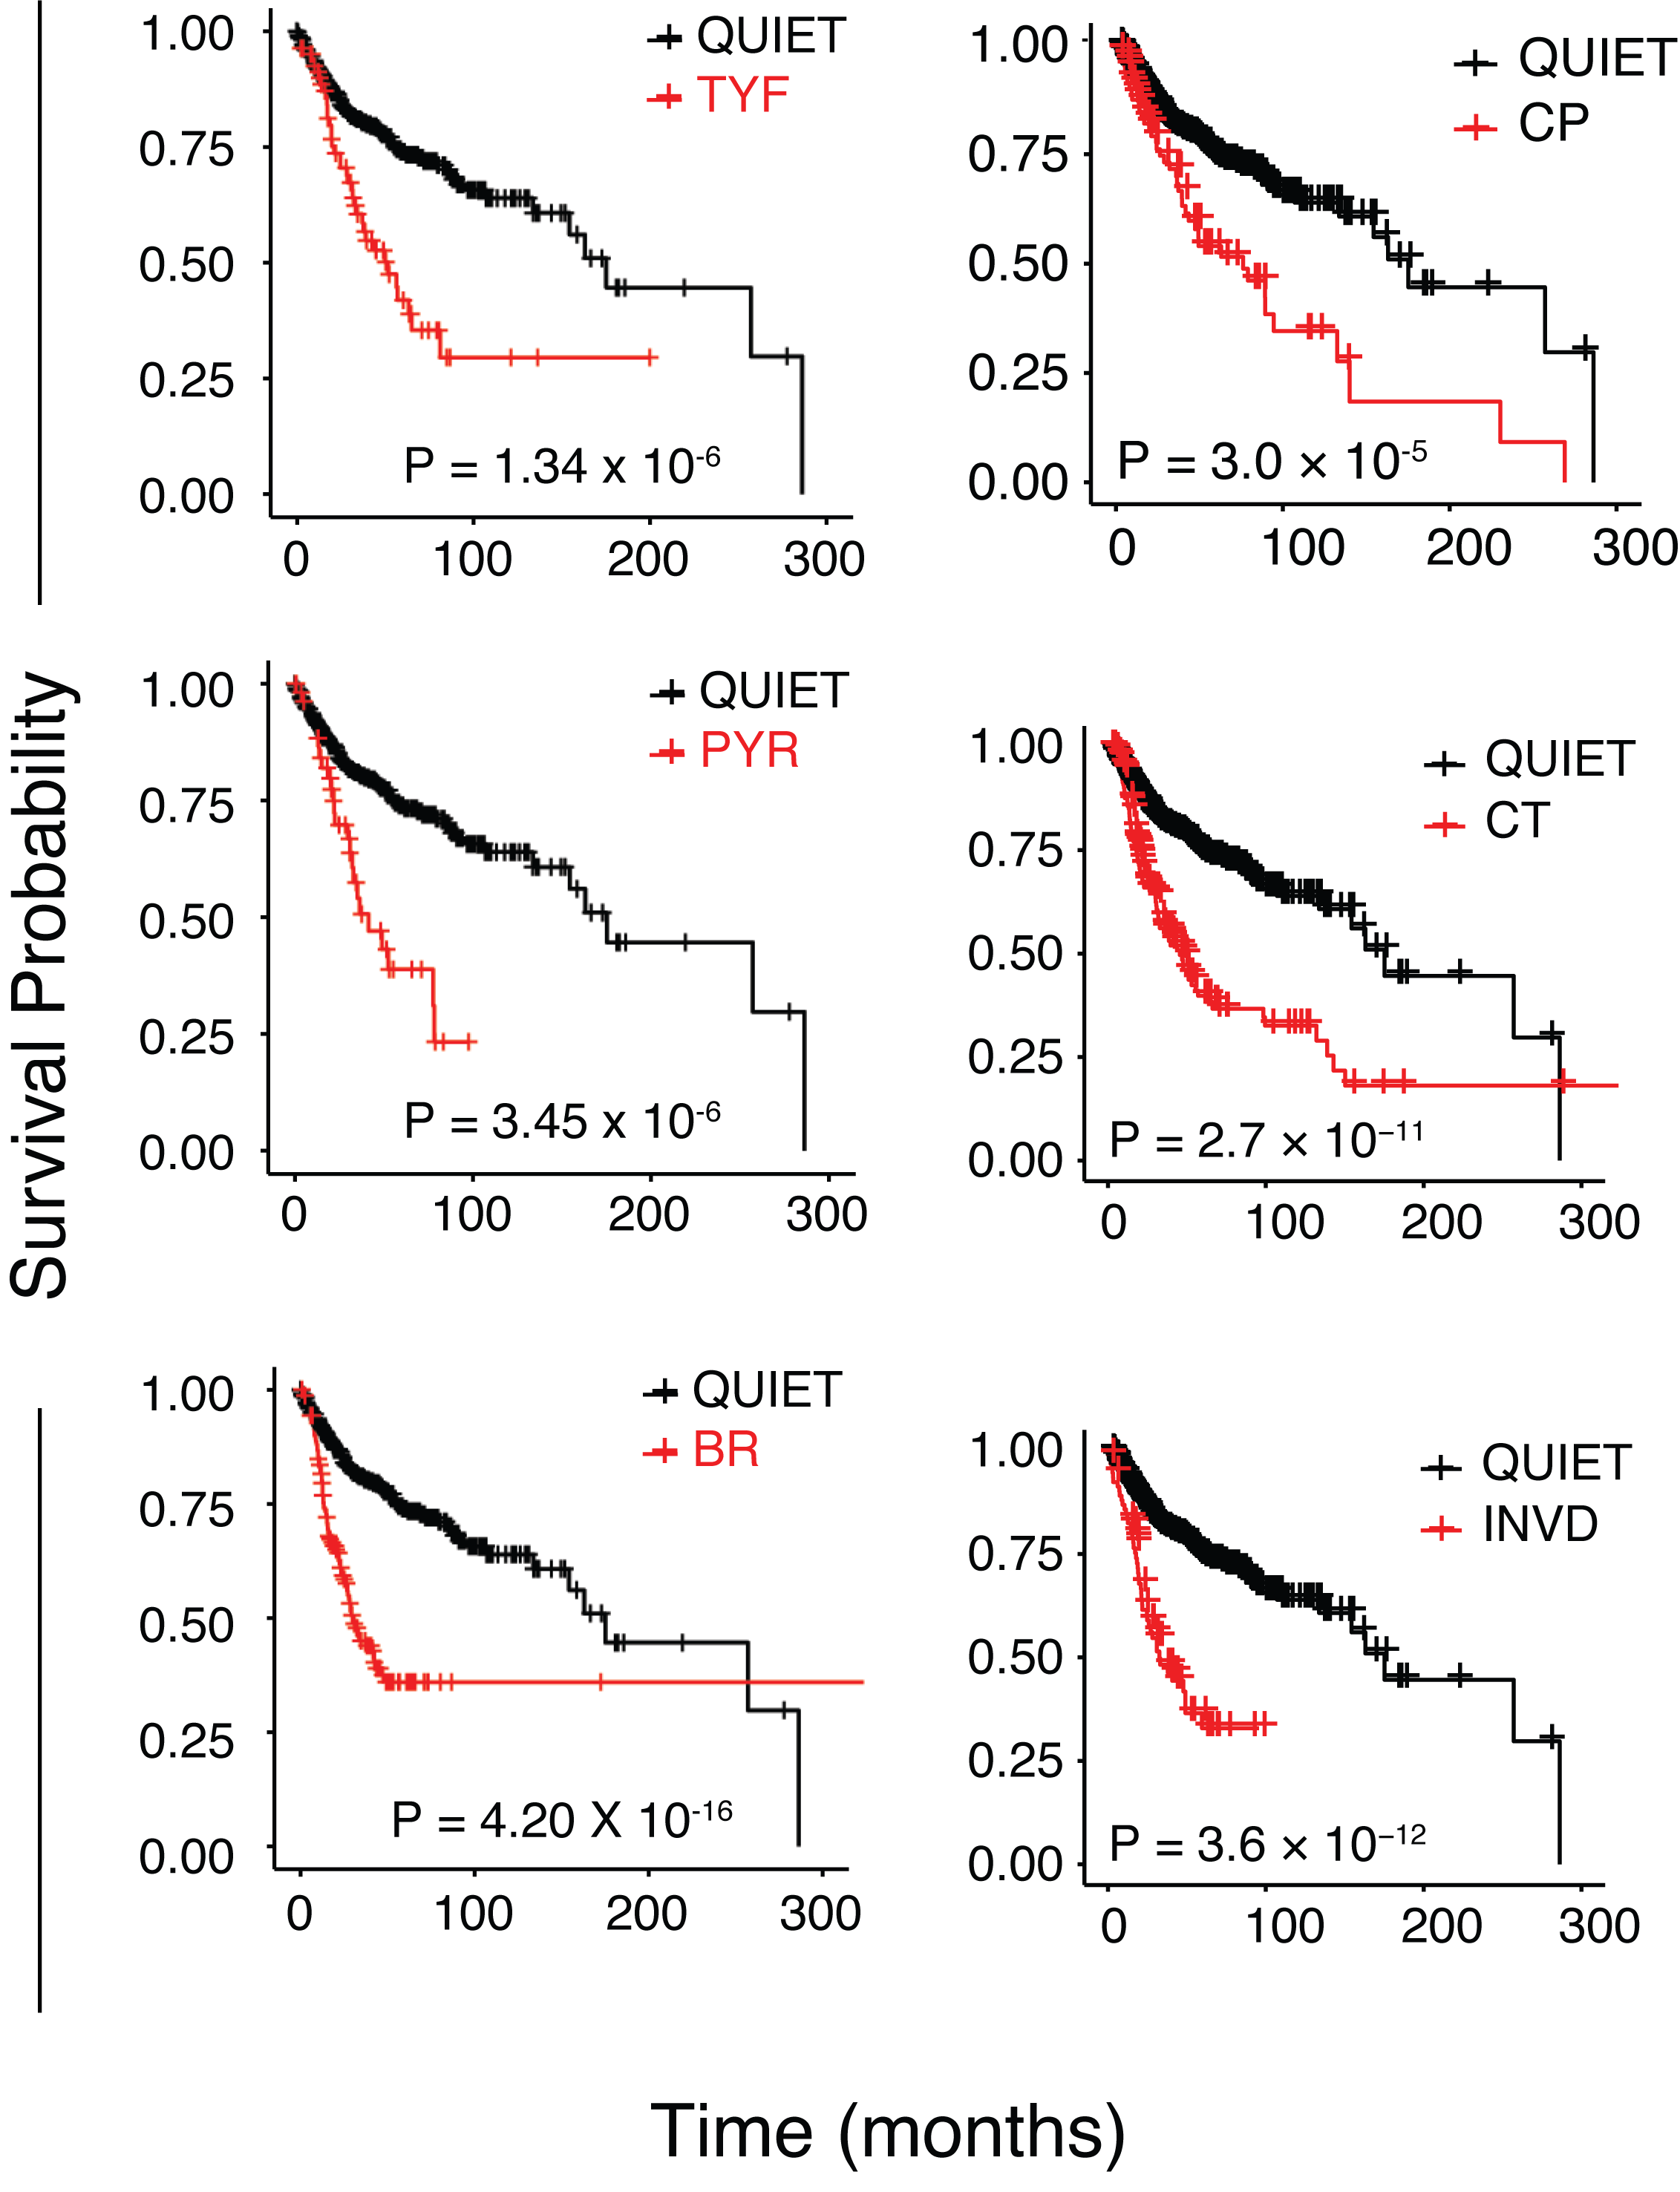
\includegraphics[width=0.95\linewidth]{figures/600ppi/clustering_km.png}
    \caption{\textbf{Overall survival worse in 6 clusters than the QUIET.}}
    \label{fig:clustering_km}
\end{figure}

\begin{figure}
    \centering
    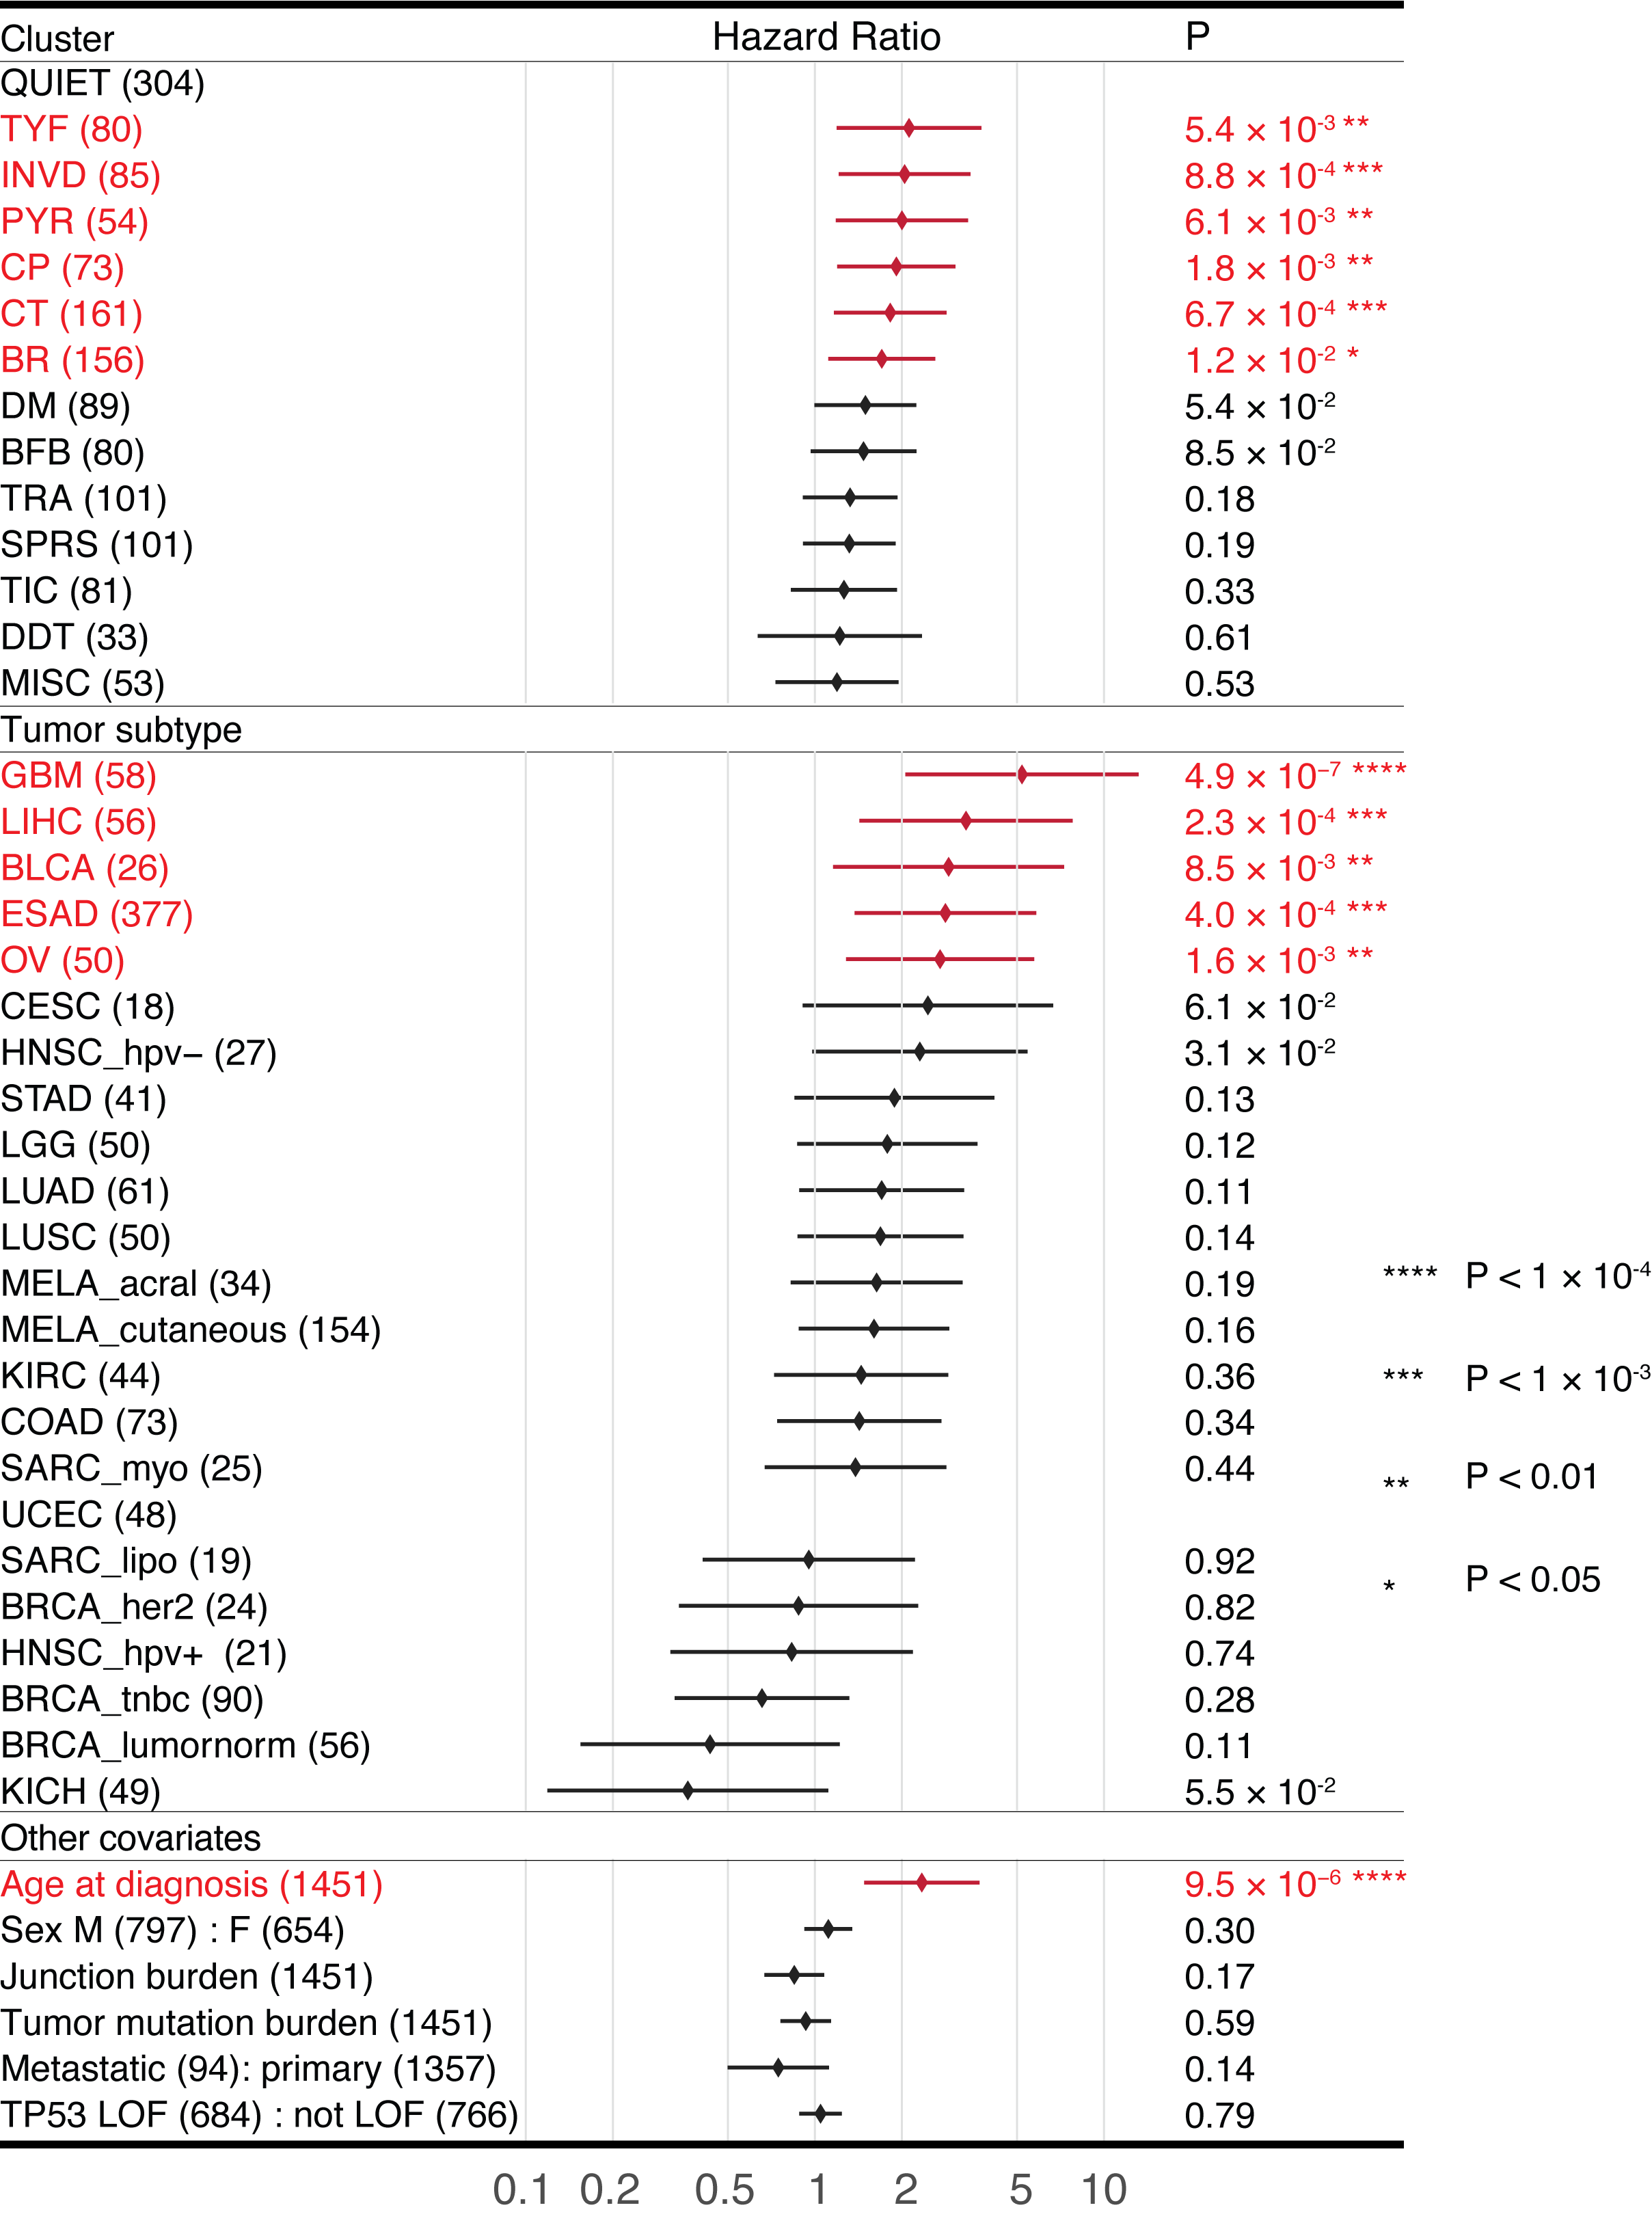
\includegraphics[height=0.95\textheight]{figures/600ppi/clustering_os_full.png}
    \caption{\textbf{Cox model correcting for covariates show the associations between TYF, INVD, PYR, CP, CT, BR and worse overall survival after correction of related covariates.}}
    \label{fig:clustering_os_cox}
\end{figure}

Tallying normalized junction counts across 13 event categories and 2,487 patients, we found 14 stable clusters using standard model selection metrics (Figure \ref{fig:find_k}). Most clusters were dominated by 1-3 event types (e.g. CT = chromothripsis, BR = BFBC, rigma, DDT = deletion, duplication, TIC) with the exception of two: QUIET (few events) and SPRS (sparse, miscellaneous events).

Consistent with previous reports, the CT cluster was significantly enriched in prostate adenocarcinoma  (PRAD, $P = \SI{2.05e-5}{}$, $OR = 1.99$, single-sided z-test, Bayesian logistic regression, \cite{Kovtun2015-kq}) and glioblastoma multiforme (GBM, $P = \SI{5.00e-8}{}$, $OR = 2.61$, \cite{Furgason2015-rv})  (Figure \ref{fig:clustering_heat_tt},\ref{fig:clustering_tt_all}). Similarly, the CP (chromoplexy) cluster was significantly enriched in PRAD ($P = \SI{2.32e-10}{}$, $OR = 3.18$, \cite{baca2013}). DDT tumors (defined by high burdens of deletions, duplications, and templated insertion chains) were enriched in triple-negative breast cancer (TNBC) ($P < \SI{2.2e-16}{}$, $OR = 8.80$),  ovarian cancers ($P = \SI{7.03e-16}{}$, $OR = 6.89$), and more broadly sex-hormone driven tumors ($P = \SI{3.18e-14}{}$, $OR = 19.0$).

Inspection of the heatmap in Figure \ref{fig:clustering_heat_tt} showed that the classes of complex SV introduced in this study (pyrgo, rigma, tyfonas) largely clustered independently from known complex SV types (double minute, BFBC, chromothripsis, chromoplexy). Among these, the BR (BFBC and Rigma dominated) cluster was primarily (60\%) composed of ESAD cases ($P < \SI{2.2e-16}{}$, $OR = 6.08$) and enriched in gastrointestinal tumors (e.g. esophageal, colorectal, and gastric adenocarcinoma) ($P < \SI{2.2e-16}{}$, $OR = 4.56$) (Figure \ref{fig:clustering_heat_tt},\ref{fig:clustering_tt_all}). The TYF (tyfonas dominated) cluster was enriched in both luminal breast cancer ($P = \SI{4.87e-8}{}$, $OR = 3.25$),  HER2+ breast cancer ($P < \SI{2.64e-9}{}$, $OR = 4.96$), dedifferentiated liposarcoma ($P < \SI{2.2e-16}{}$, $OR = 24.5$), and acral melanoma ($P < \SI{1.84e-15}{}$, $OR = 7.40$). In contrast, cutaneous melanomas were enriched in the CT cluster.  Additional associations are shown in Figure \ref{fig:clustering_tt_all} and \cite{Hadi2020-um} Table S3.

We associated somatic or constitutional genotypes in COSMIC Cancer Gene Census genes with cluster membership, after correcting for tumor subtype as a covariate. More than 20\% of cases in the DDT cluster harbored constitutional ($P = \SI{1.60e-4}{}$, $OR = 3.81$) loss of function lesions in \textit{BRCA1} (Figure \ref{fig:clustering_geno}). BR-cluster tumors were also significantly enriched in somatic \textit{TP53} mutations ($P < \SI{4.71e-7}{}$, $OR = 2.06$). Additional somatic genotype associations (Figure \ref{fig:clustering_geno_all}), including an enrichment of \textit{SMC4} ($P = \SI{2.33e-3}{}$, $OR = 3.11$) and \textit{RAD21} ($P = \SI{1.96e-3}{}$, $OR = 3.27$) mutations in the INVD (inverted duplication dominant) cluster, \textit{ARID1A} ($P = \SI{1.21e-3}{}$, $OR = 1.86$) mutations in the TIC (templated insertion chain dominant) cluster, and \textit{KMT2C} ($P = \SI{2.89e-3}{}$, $OR = 1.95$) mutations in the TRA (translocation-dominated) cluster.

Compared to QUIET cluster, Kaplan-Meier analysis revealed poorer survival among novel SV-class dominated clusters (BR, PYR, and TYF; FDR $<$ 0.1, log rank test) as well as several clusters dominated by previously-described SV classes (CP, CT, and INVD; Figure \ref{fig:clustering_km}). These effects persisted after correcting for clinical and molecular covariates in a Cox regression analysis, with BR ($P = \SI{1.17e-2}{}$, $HR = 1.72$, likelihood ratio test, Cox regression), PYR ($P = \SI{6.13e-3}{}$, $HR = 2.01$), TYF ($P = \SI{5.37e-3}{}$, $HR = 2.12$ , CP ($P = \SI{1.76e-3}{}; HR = 1.91$), CT ($P = \SI{6.69e-4}{}; HR = 1.83$), and INVD ($P = \SI{8.79e-4}{}; HR = 2.06$) clusters each demonstrating reduced survival relative to the QUIET cluster (Figure \ref{fig:clustering_os_cox}).

\section{Discussion}
Our comprehensive analysis of 2,778 genome graphs establishes JCN topology as a key signal for the classification of complex SVs in human cancer. The regional, genotypic, and tumor type distribution of SV classes nominated in this study (pyrgo, rigma, tyfonas) are distinct from previously identified complex rearrangement patterns (chromothripsis, chromoplexy, BFBC), suggesting that they represent novel mutational processes and/or foci of somatic selection.  We anticipate that these findings, combined with JaBbA's superior performance relative to previous CNA algorithms, will bring the genome graph paradigm to the mainstream of cancer genome analysis.

Our data show that rigma likely arise from early and ongoing accumulation of DEL-like junctions at large and late replicating genes.  Though rigma are overrepresented among  previously annotated fragile sites defined by cell culture experiments \cite{schwartz2006,fungtammasan2012, ohta1996, Ma2012-ym}, the majority of rigma actually fall outside of these loci.  An intriguing possibility is that rigma identified in our study represent previously unannotated \textit{in vivo} genomic fragile sites. If so, future studies examining somatic rigma patterns as lineage-specific readouts of human genome fragility may shed insight into the biology of aging and developmental disease (e.g. autism, neurodegenerative conditions).

Previous studies have linked fragile sites to replication-transcription collisions in transcriptionally active genes \cite{Helmrich2011-yj,Wilson2015-zg,Blin2019-kf}.  The significant recurrence of rigma at \textit{FHIT} and other fragile-site associated genes (e.g. \textit{WWOX}, \textit{MACROD2}) even after correcting for covariates suggests that replication timing and gene size do not fully account for their accumulation in hotspots.   The preference of rigma for ESAD (and more broadly, GI adenocarcinomas) suggests that somatic rigma patterns in GI cancers may reflect epigenetic states of cell types in the healthy GI epithelium, which may be revealed through further study via single cell approaches or cell sorting and chromatin profiling.

While  a subset of pyrgo hotspots (e.g. \textit{MYC} superenhancers) may be functional and under positive somatic selection, the association of pyrgo with superenhancers is more likely due to a neutral mutational process that predisposes enhancers to (nested) duplications.  Recent work suggests that enhancers may form cooperative multivalent chromatin structures \cite{Hnisz:2017fz}, some of which may be prone to characteristic breakage and repair patterns \cite{canela2017}. Further studies combining WGS and chromatin profiling in the same tumor sample will be required to assess the functional role of pyrgo formation in the evolution of cancer chromatin.  More broadly, the explicit consideration of rigma and pyrgo patterns in future statistical background models of SV recurrence will be required to accurately nominate cancer driver loci in large cancer WGS datasets.

Though tyfonas likely represent the footprint of supernumerary rings in dedifferentiated liposarcomas, their prevalence in tumor types (e.g. acral melanomas, breast cancers) not commonly associated with supernumerary rings suggest that the cytogenetic footprint of this event may be more diverse. If our Hi-C, optical mapping, and FISH-based model of tyfonas (\textbf{Fig. \ref{fig:Figure6}E}) generalizes, a key question is how these chromosomally integrated loci acquire such a wide breadth of JCN in \textit{cis}. We speculate that this allelic configuration may require a transient extrachromosomal phase, enabling the progressive self-assembly of many linear fragments ligating and duplicating in parallel across successive cell cycles.  These asymmetrically segregating shards may preferentially ligate with their sister shard in end-to-end orientation after each S phase, which may give rise to the tyfonas-associated fold back inversion pattern.

The enrichment of breakend hypermutation across multiple non-APOBEC associated SNV contexts in tyfonas suggests that these junctions may arise in a specific mutagenic cellular environment.  Though we cannot rule out the role of APOBEC enzymes in generating these SNV patterns (e.g. within a non-canonical context), they may also arise through error prone Pol-$\alpha$ fill-in or alt-NHEJ repair, both of which are active at unprotected DNA ends and generate mutations across a wide spectrum of trinucleotide contexts \cite{sfeir2012,Mirman:2018jm}.  We anticipate that future investigations in model systems will resolve some of these exciting mechanistic questions regarding tyfonas genesis.

Our study provides a template for integrating short-read WGS with long-range genome profiling to study patterns of somatic junction phase and allelic multiplicity in complex loci. Future studies that utilize long-range whole genome profiles (10X Chromium WGS, Pacific Biosciences, Oxford Nanopore Technologies, Hi-C, Bionano \mbox{\cite{Sedlazeck2018-ix}}) to phase highly rearranged somatic alleles may provide a more granular classification and mechanistic insight into complex SV mutational processes.  Larger short-read meta-analyses spanning >10,000 cancer genome graphs, which may be imminently possible through the combination of our approach and dataset with PCAWG (1,493 additional tumors) \cite{pcawg_marker2020-yi}, Hartwig Medical Foundation (4000+ cases, \cite{Priestley:20196a6}), and emerging WGS precision medicine efforts will help link novel features of genome-graph topology with clinical variables, including therapeutic response. This includes future investigations linking the presence of tyfonas to the efficacy of immune checkpoint inhibition in acral melanoma or other tumor types in which these events are found (e.g. small cell lung cancer).


%%%%%%%%%%%%%%%%%%%%%%%%%%%%%%%%%%%%%%%%%%%%%%%
%% Chapter 4: SV evolution after telomere crisis
%%%%%%%%%%%%%%%%%%%%%%%%%%%%%%%%%%%%%%%%%%%%%%%
\chapter{Structural variant evolution after telomere crisis} \label{chap:tel_crisis} 
In this chapter I set out to capture the SV events in human cell lines directly resulting from natural telomere crisis. Sally Dewhurst designed and created the \textit{in vitro} telomere crisis model, executed all the experiments, and analyzed the data except for the WGS parts. Huasong Tian prepared WGS libraries.

% \section{Introduction}

\section{Genomic complexity after spontaneous telomerase activation}

\begin{figure}
    \centering
    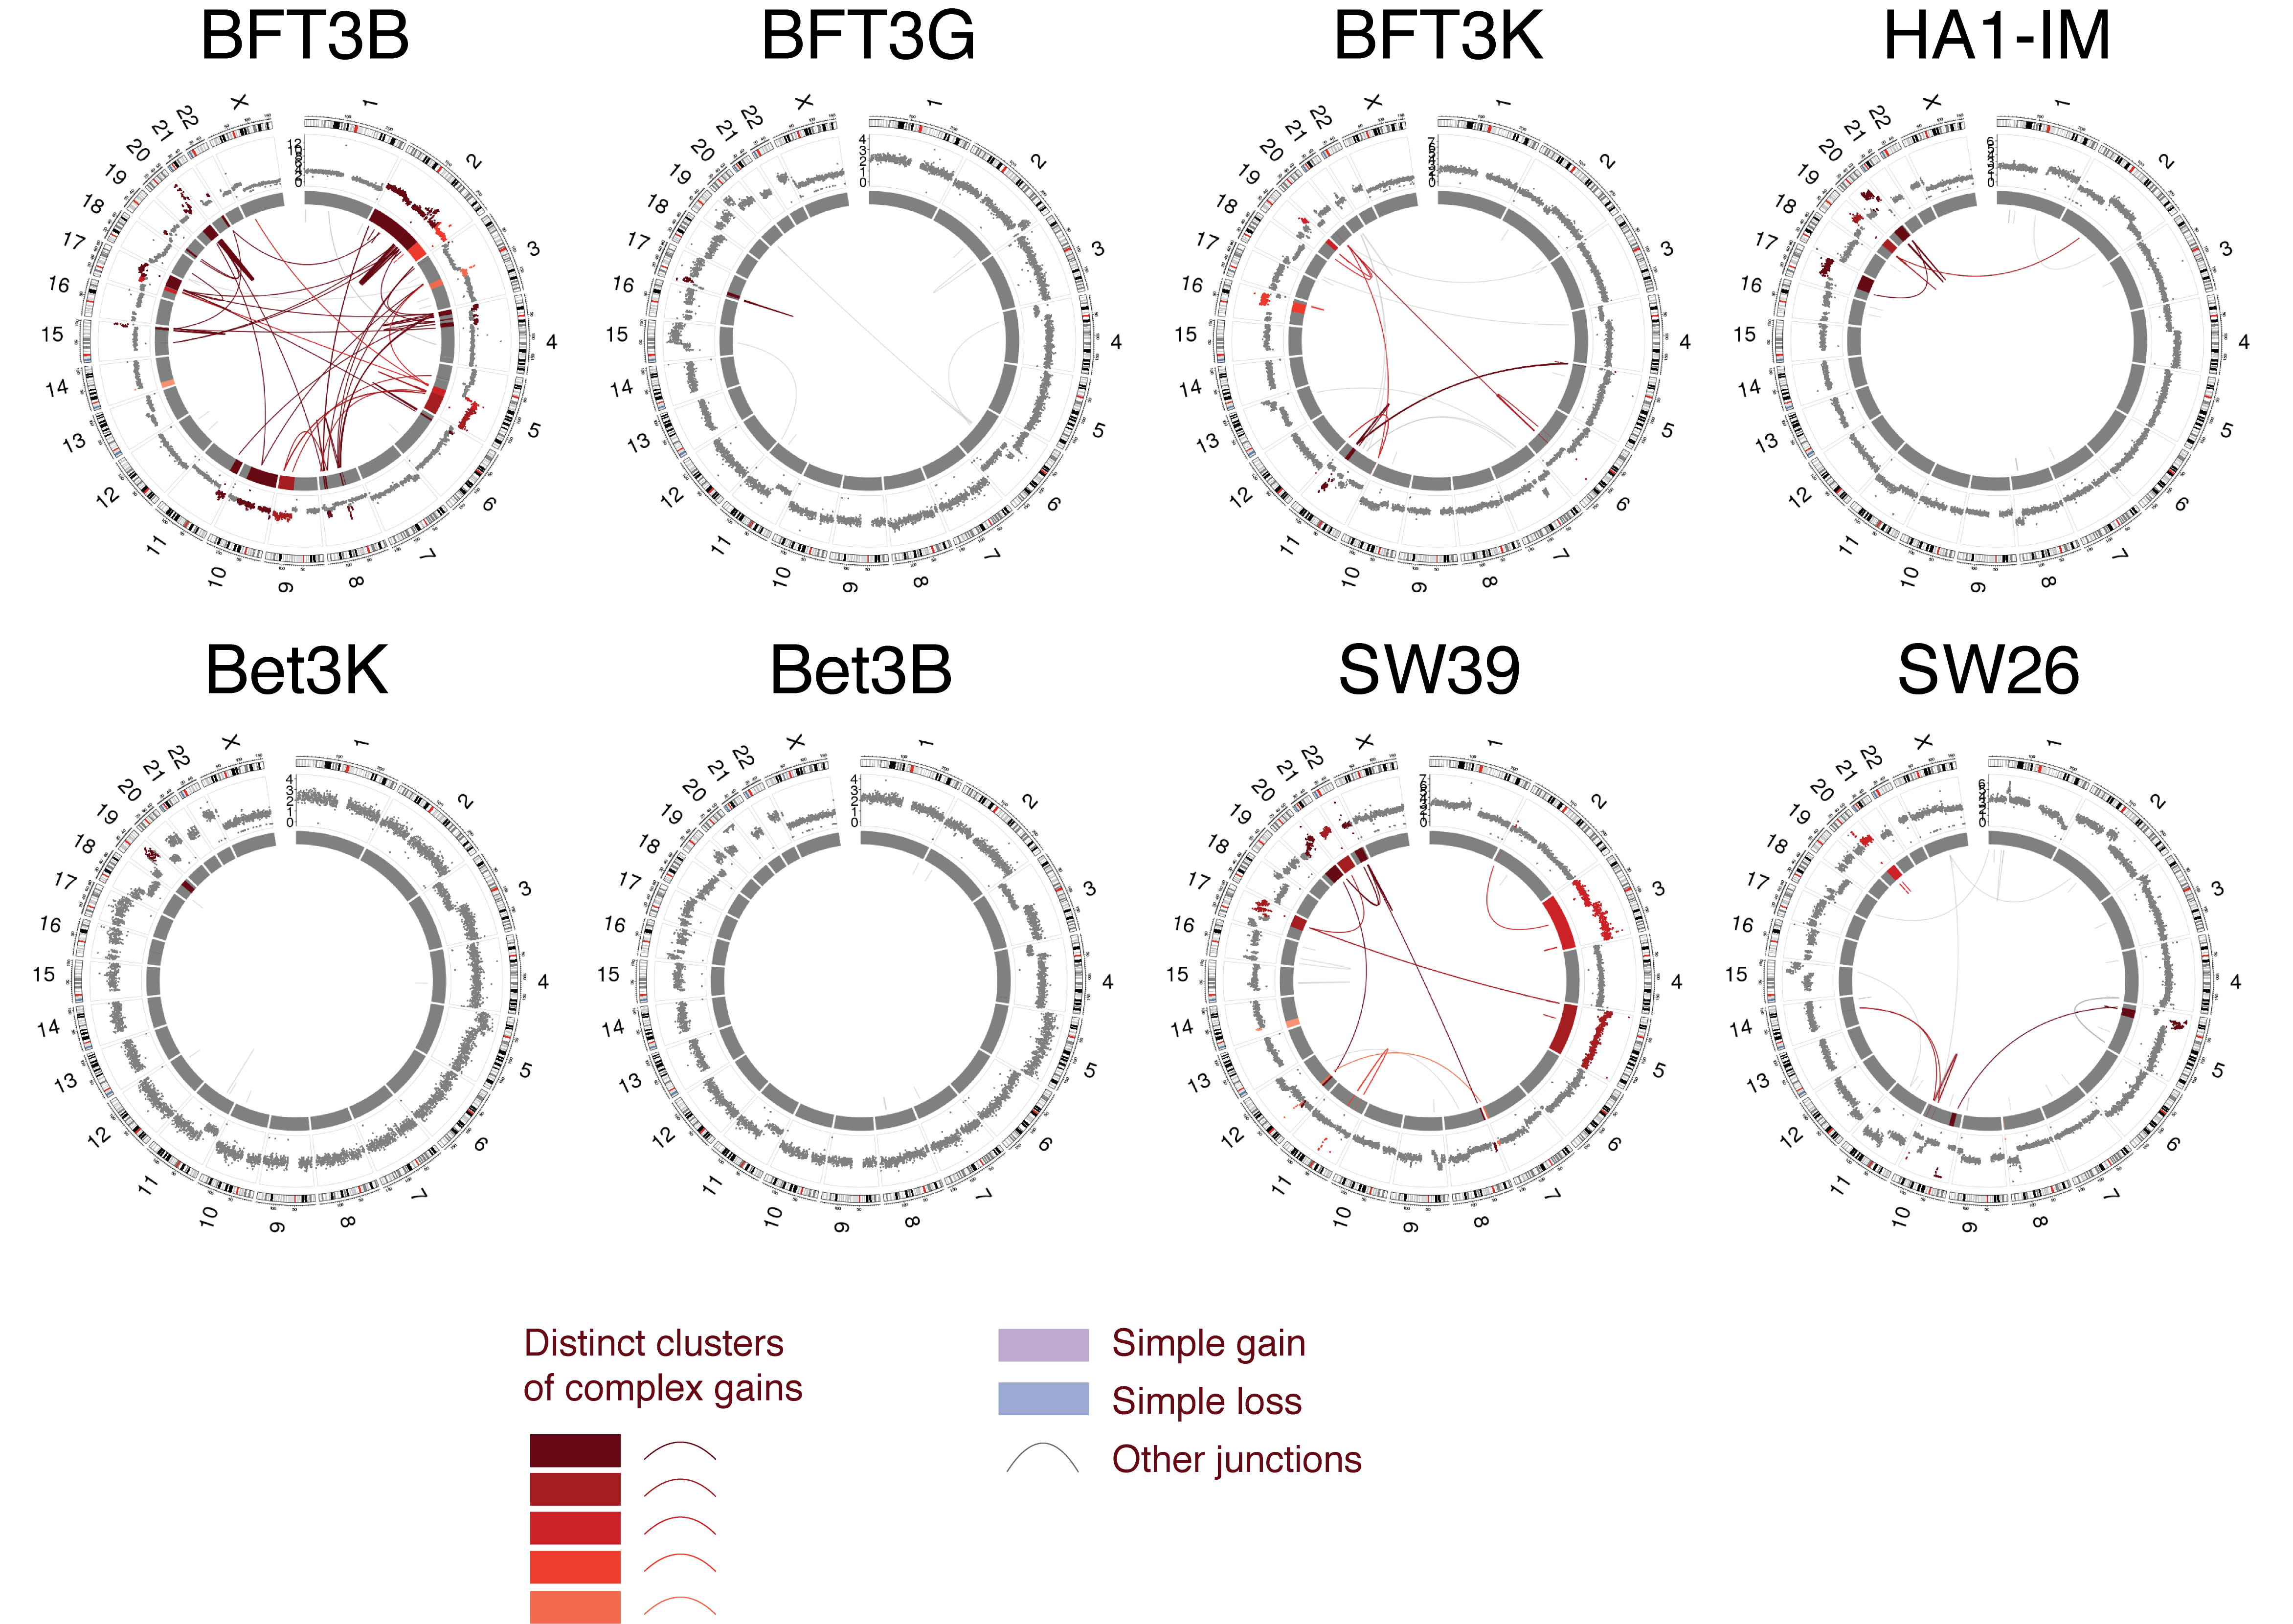
\includegraphics[width=0.95\linewidth]{figures/600ppi/tc_prev_circos.png}
    \caption{\textbf{Post-crisis SV landscape in 8 spontaneously drived cell lines.}}
    \label{fig:tc_prev_circos}
\end{figure}

\begin{figure}
    \centering 
    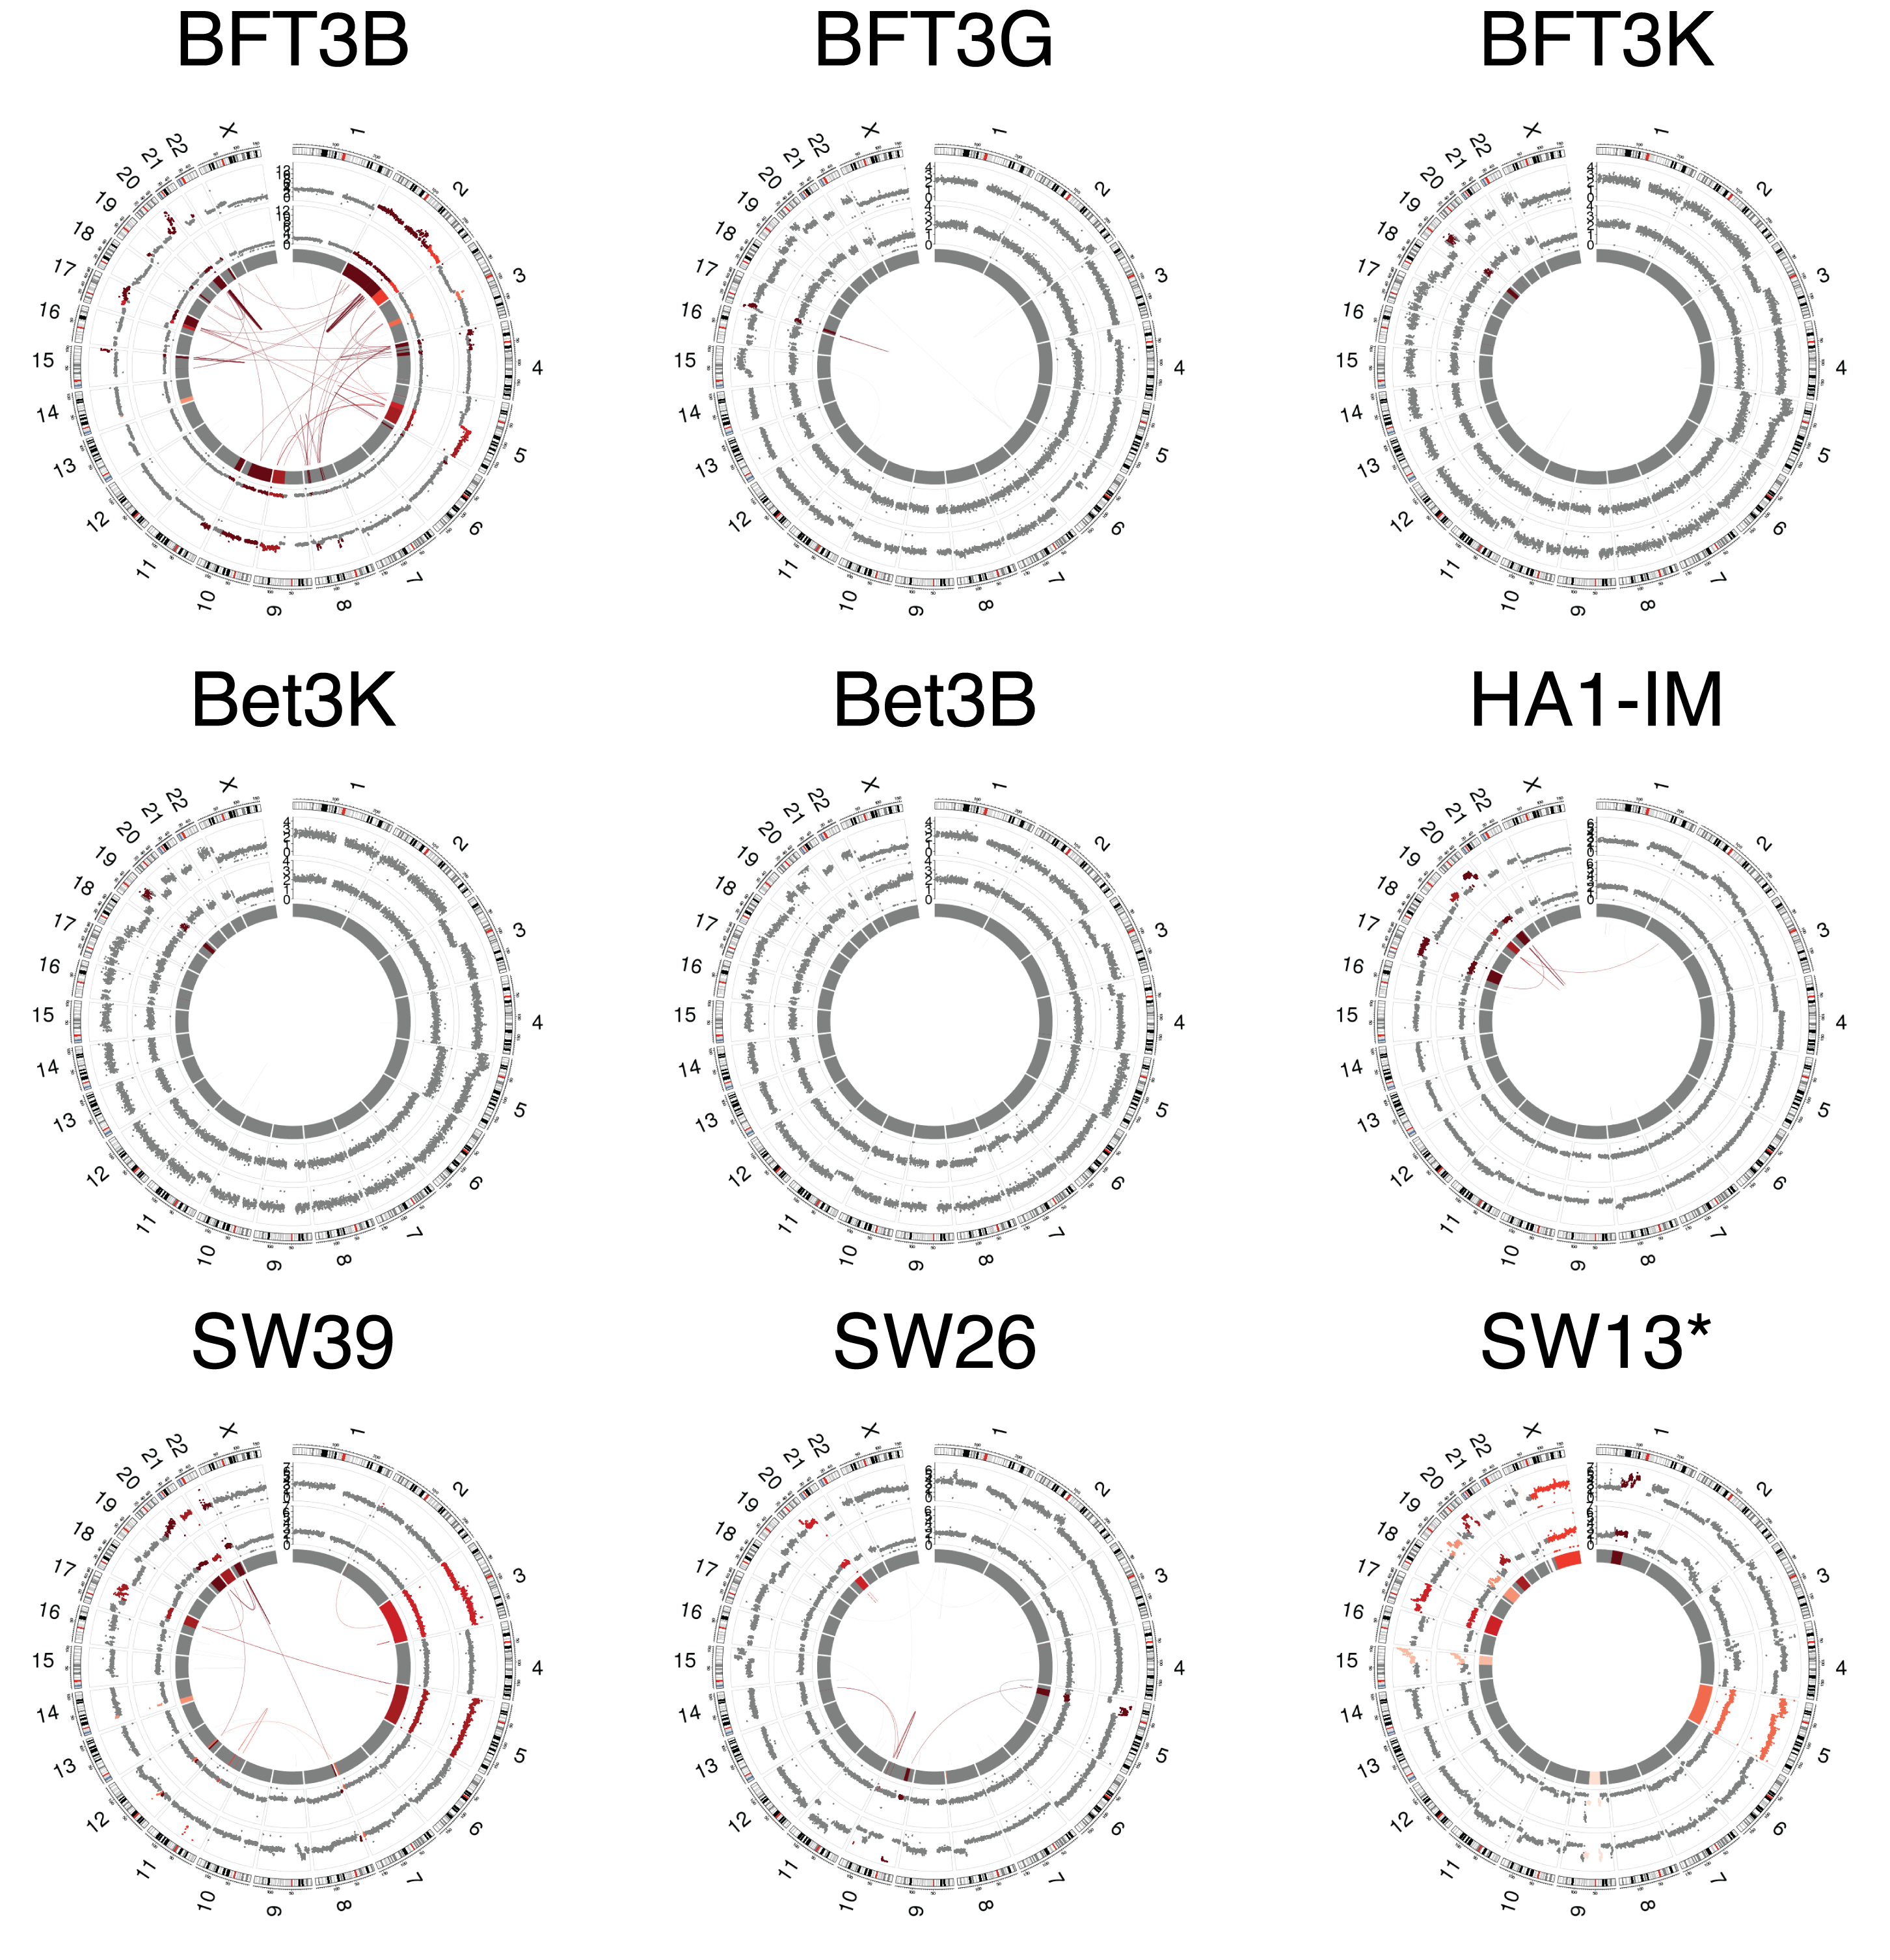
\includegraphics[width=0.95\linewidth]{figures/600ppi/tc_prev_all_circos.png}
    \caption{\textbf{Post-crisis SV landscape with pre-crisis whole genome coverage in 9 spontaneously drived cell lines.}}
    \label{fig:tc_prev_all_circos}
\end{figure}

\begin{figure}
    \centering
    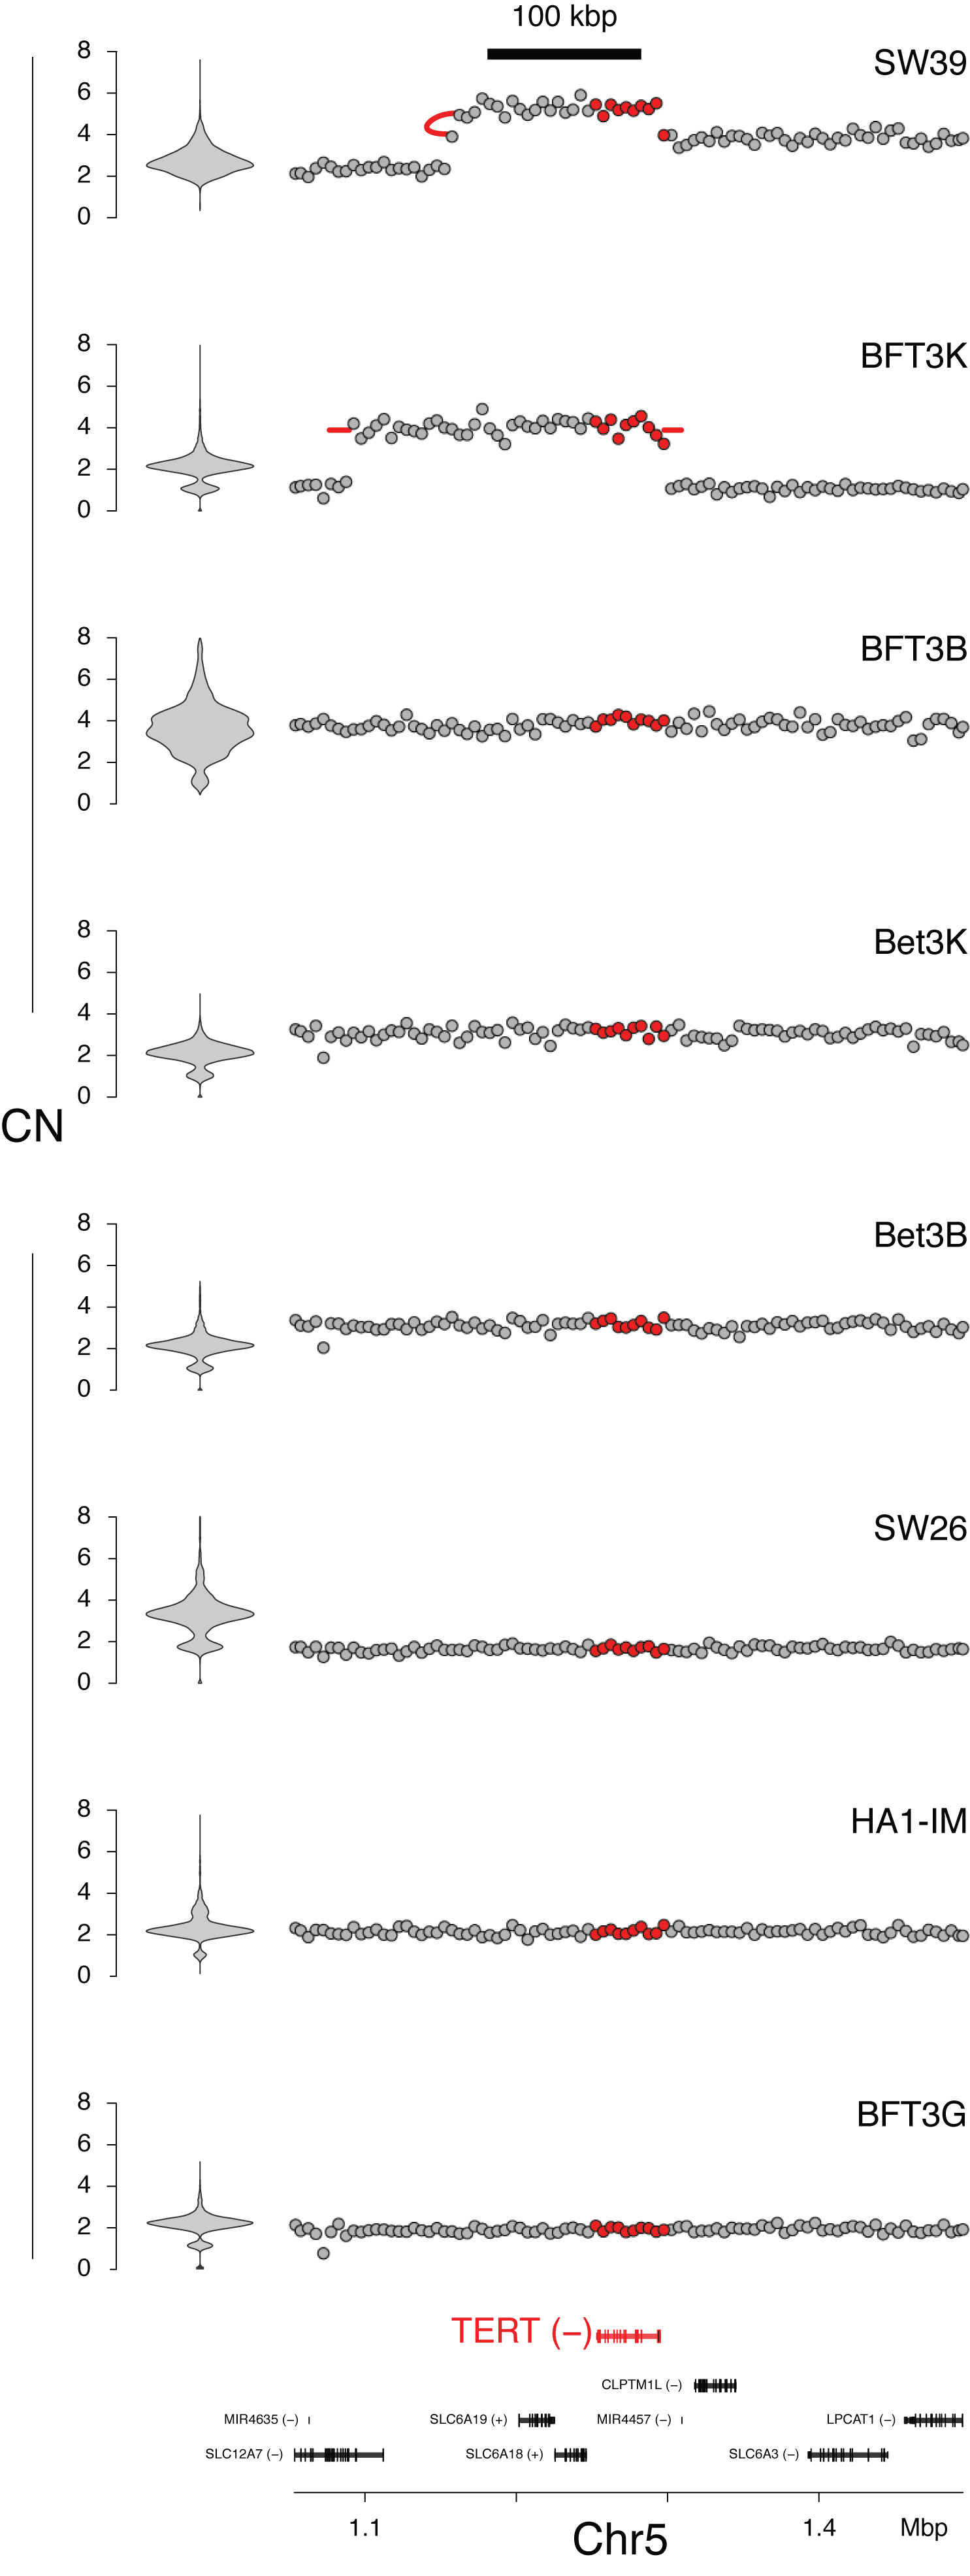
\includegraphics[height=0.95\textheight]{figures/600ppi/tc_prev_tert.png}
    \caption{\textbf{SVs around TERT locus in spontaneous post-crisis cell lines.}}
    \label{fig:tc_prev_tert}
\end{figure}

\begin{figure}
    \centering
    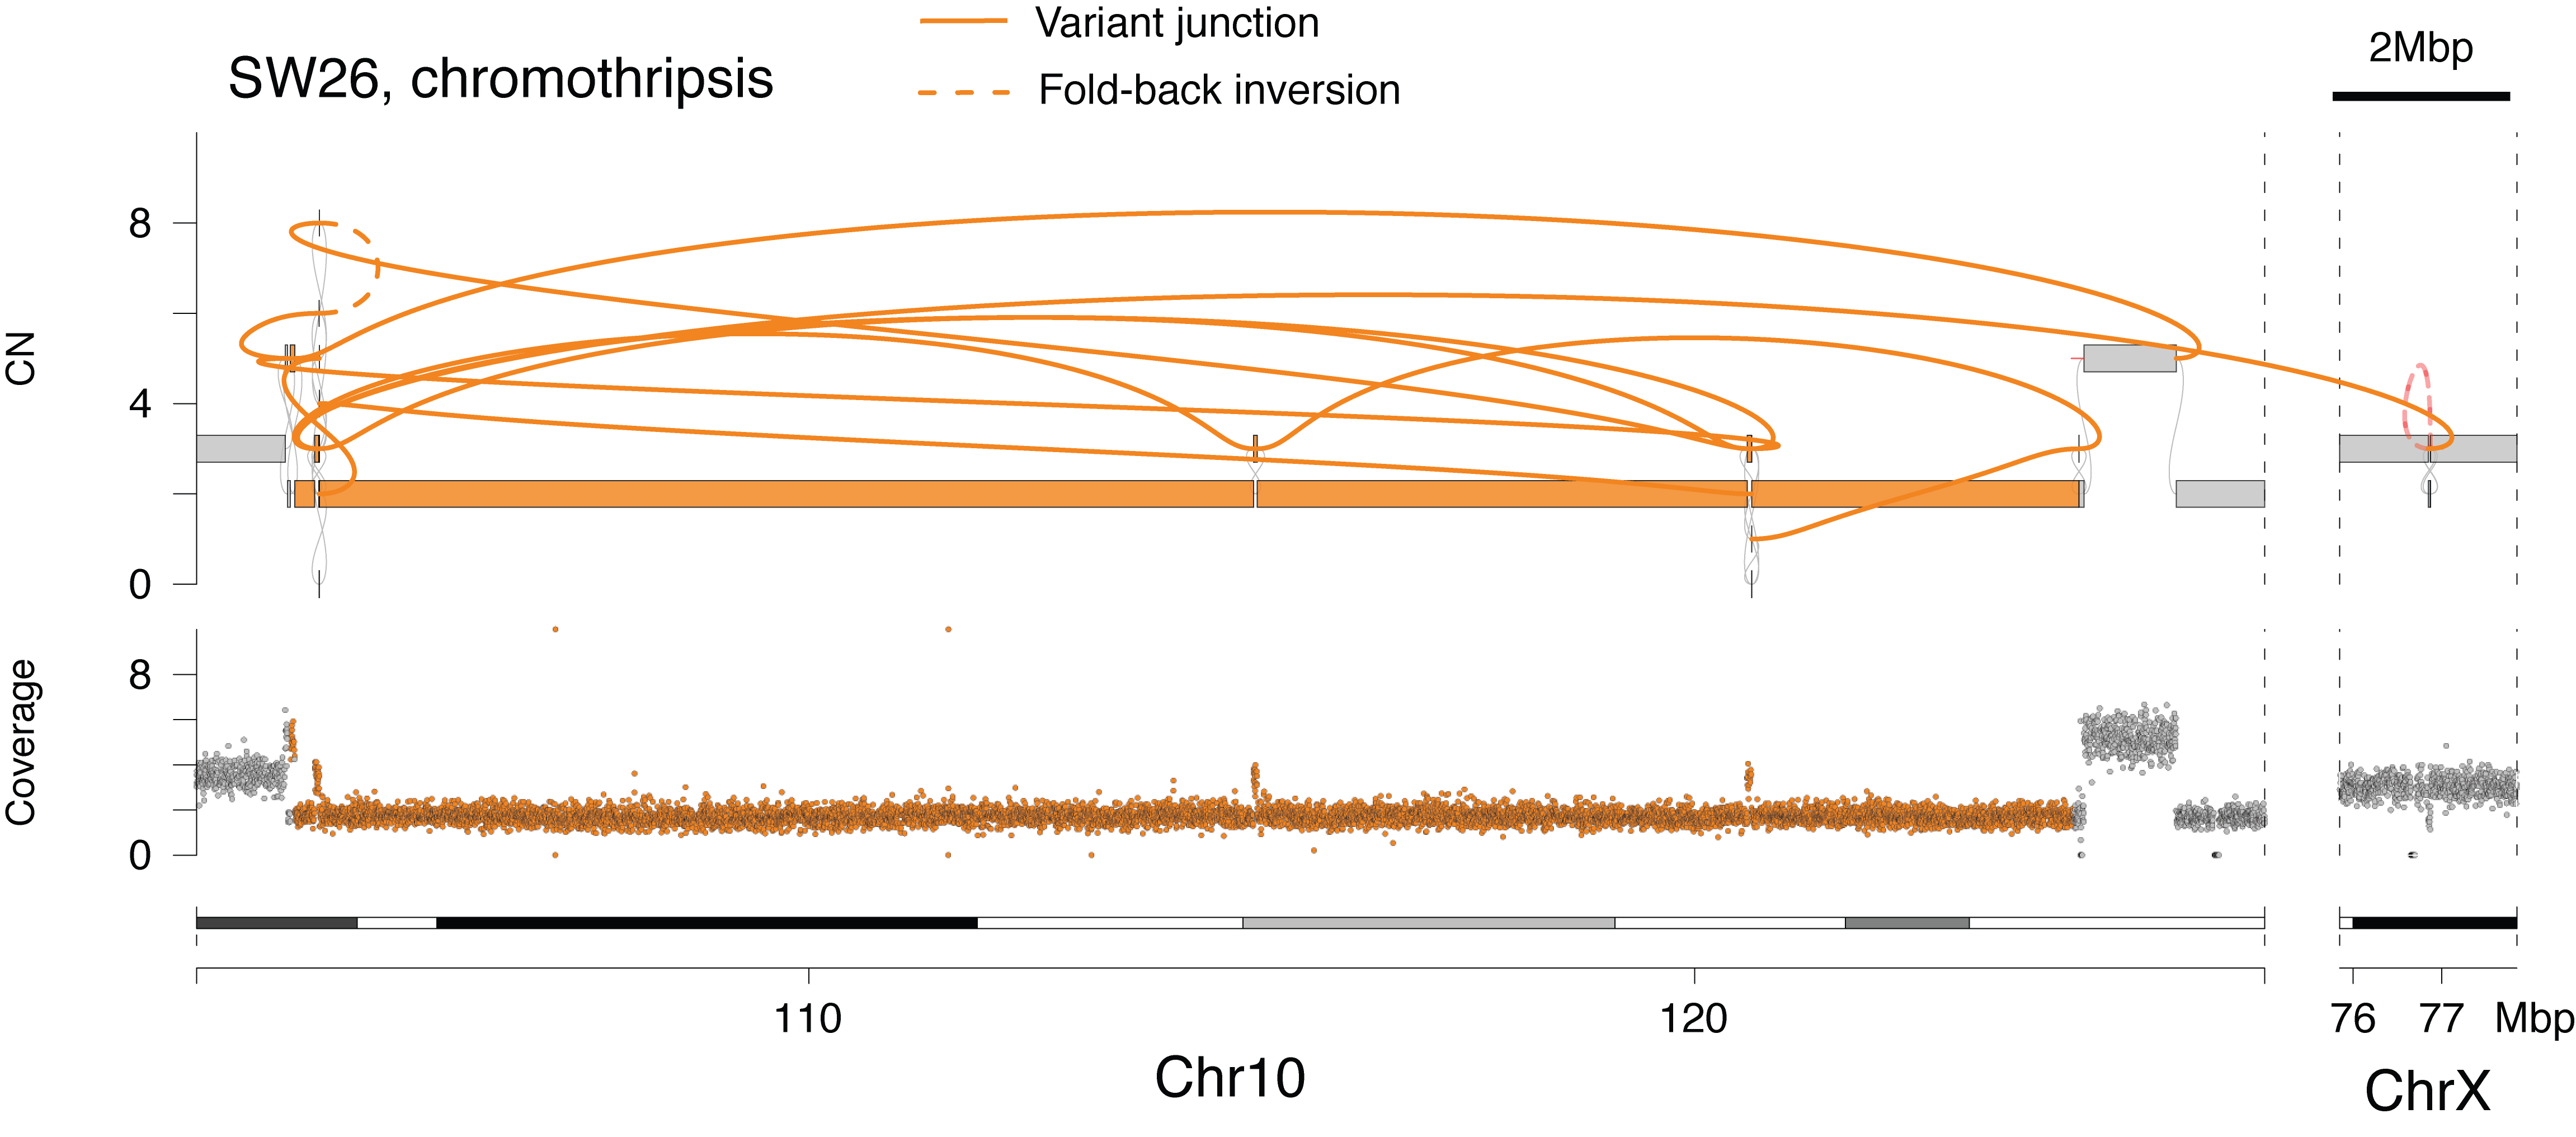
\includegraphics[width=0.95\linewidth]{figures/600ppi/tc_fig1b_ct_sw26.png}
    \caption{\textbf{Chromothripsis event in SW26 cell line.}}
    \label{fig:tc_ct_sw26}
\end{figure}

\begin{figure*}
    \centering
    \includegraphics[width=0.95\linewidth]{figures/600ppi/tc_bft3k_bfb.png}
    \caption{\textbf{Primitive BFB event in BFT3K cell line.}}
    \label{fig:tc_bft3k_bfb}
\end{figure*}

\begin{figure*}
    \centering
    \includegraphics[width=0.95\linewidth]{figures/600ppi/tc_bft3b_complex.png}
    \caption{\textbf{Complex amplification event in BFT3K cell line.}}
    \label{fig:tc_bft3b_complex}
\end{figure*}

% TODO: add table of the nine SV40T cell lines
In order to determine the SVs in post-telomere crisis genomes, we examined nine SV40 large T-transformed cell lines that had undergone spontaneous telomerase activation after passage into telomere crisis (Figure \ref{fig:tc_prev_circos}, \ref{fig:tc_prev_all_circos}). The cell lines represent independent immortalization events in a variety of cell lineages \cite{Bryan1995-ik,Shay1989-ua,Counter1992-yg}. We carried out whole genome sequencing of these nine post-crisis cell lines and their pre-crisis counterparts to a median depth of 40X (range: 15-51) and generated junction-balanced genome graphs\cite{Hadi2020-um} via JaBbA from SvABA\cite{Wala2018-qa} and GRIDSS\cite{Cameron2021-db} junction calls (see \ref{app:tc_wgs_processing}).

Using short-read WGS data, JaBbA optimally assigns a copy number to both vertices (intervals) and edges (junctions, adjacencies) of genome graphs by fitting a probabilistic model to binned genome-wide read depth. These graphs obey a basic stoichiometric constraint of DNA dosage, namely that every copy of every (interstitial) segment must have a left and a right neighbor. The topology of these genome graphs can be further analyzed to identify simple and complex SV events, including chromothripsis and BFB cycles.

Comparison of ancestral (pre-crisis) and derived (post-crisis) genome graphs showed that eight of nine post-crisis cell lines acquired virtually all (61.9\% - 100\%, median 96.6\%) of their observed structural variation during or after crisis (Figure \ref{fig:tc_prev_circos}, \ref{fig:tc_prev_all_circos}). One cell line (SW13) had acquired significant aneuploidy and genome rearrangement prior to crisis and was therefore difficult to interpret (Figure \ref{fig:tc_prev_all_circos}). The other eight post-crisis genome graphs demonstrated varying levels of aneuploidy (ploidy ranges: 1.9-3.4) with variable numbers of clonal junctions per genome (range: 5-115, median 25). Analysis of junction-balanced genome graphs \cite{Hadi2020-um} revealed complex multi-chromosomal gains in six samples, with the other two lines harboring only broad arm level losses or gains (Figure \ref{fig:tc_prev_circos}).

Strikingly, besides one instance of chromothripsis (Figure \ref{fig:tc_ct_sw26}), genome graph-based categorization of complex SVs \cite{Hadi2020-um} identified few classic footprints of chromothripsis or BFB cycles in these genomes. However, several amplified subgraphs were associated with stepwise copy number gains reminiscent of BFB cycles (Figure \ref{fig:tc_bft3k_bfb}). The majority of copy changes in these subgraphs could not be attributed to fold-back inversion junctions (a hallmark of BFB cycles) but were instead driven by a spectrum of duplication and translocation-like junctions and templated insertion chains. These patterns are exemplified in a 10 Mbp region of 20q of post-crisis cell line BFT3B that is amplified to 10-15 copies, incorporating Mbp scale fragments from 11 other chromosomes at lower copy number including chromosome 8 and 19 (Supplementary Figure \ref{fig:tc_bft3b_complex}). Of note, five of eight cell lines showed modest increases in TERT copy number, providing a possible genomic basis for escape from telomere crisis (Figure \ref{fig:tc_prev_tert}).

In summary, across the eight post-crisis cell lines, spontaneous escape from crisis was associated with a highly variable spectrum of SV patterns, ranging from relatively unaltered genomes to complex non-canonical patterns of amplification as well as numerical gains and losses. Importantly, BFB-like patterns and chromothripsis were not a general feature of the post-crisis genomes.

\section{An in vitro system for telomerase-mediated escape from natural telomere crisis}
\begin{figure}
    \centering
    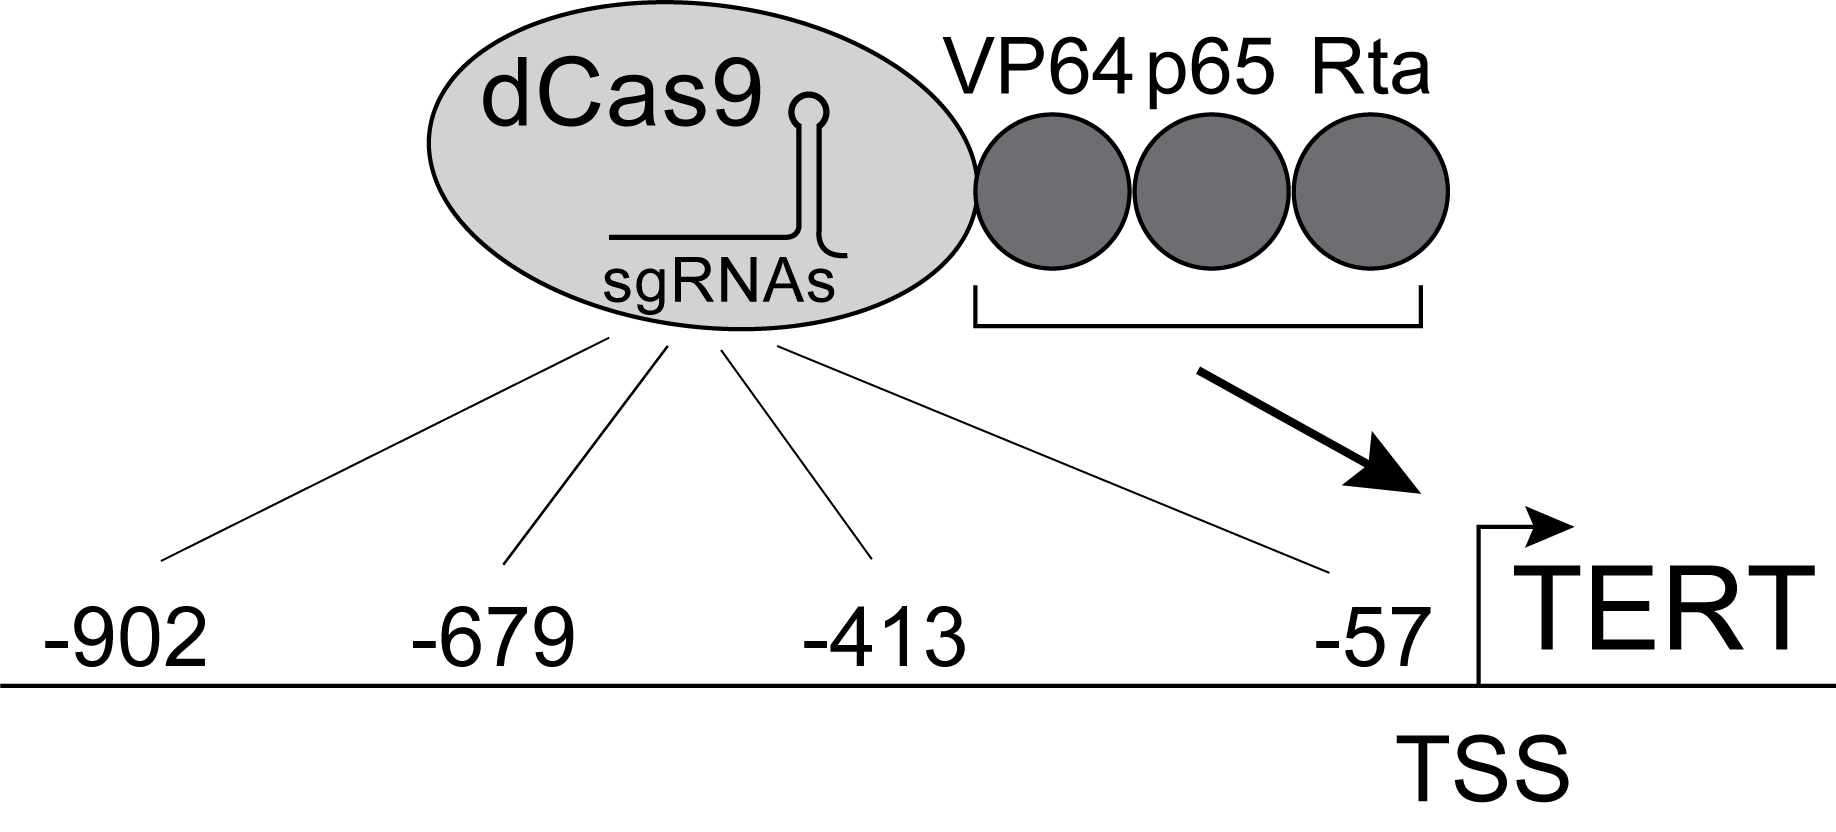
\includegraphics[width=0.95\linewidth]{figures/600ppi/tc_system.png}
    \caption{\textbf{\textit{In vitro} iCRISPRa system to activate endogeneous TERT expression}}
    \label{fig:tc_system}
\end{figure}

\begin{figure}
    \centering
    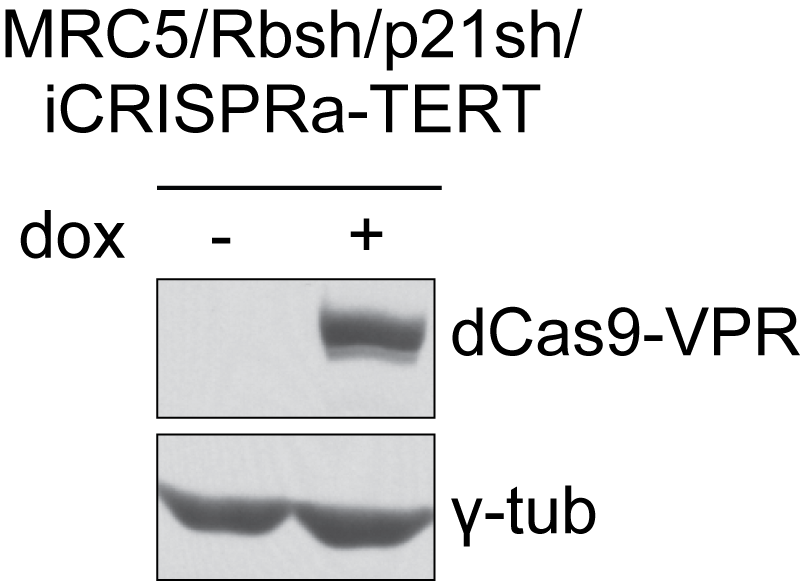
\includegraphics[width=0.95\linewidth]{figures/600ppi/tc_tert_western.png}
    \caption{\textbf{Detection of TERT protein after doxycycline induction.}}
    \label{fig:tc_tert_western}
\end{figure}

\begin{figure}
    \centering
    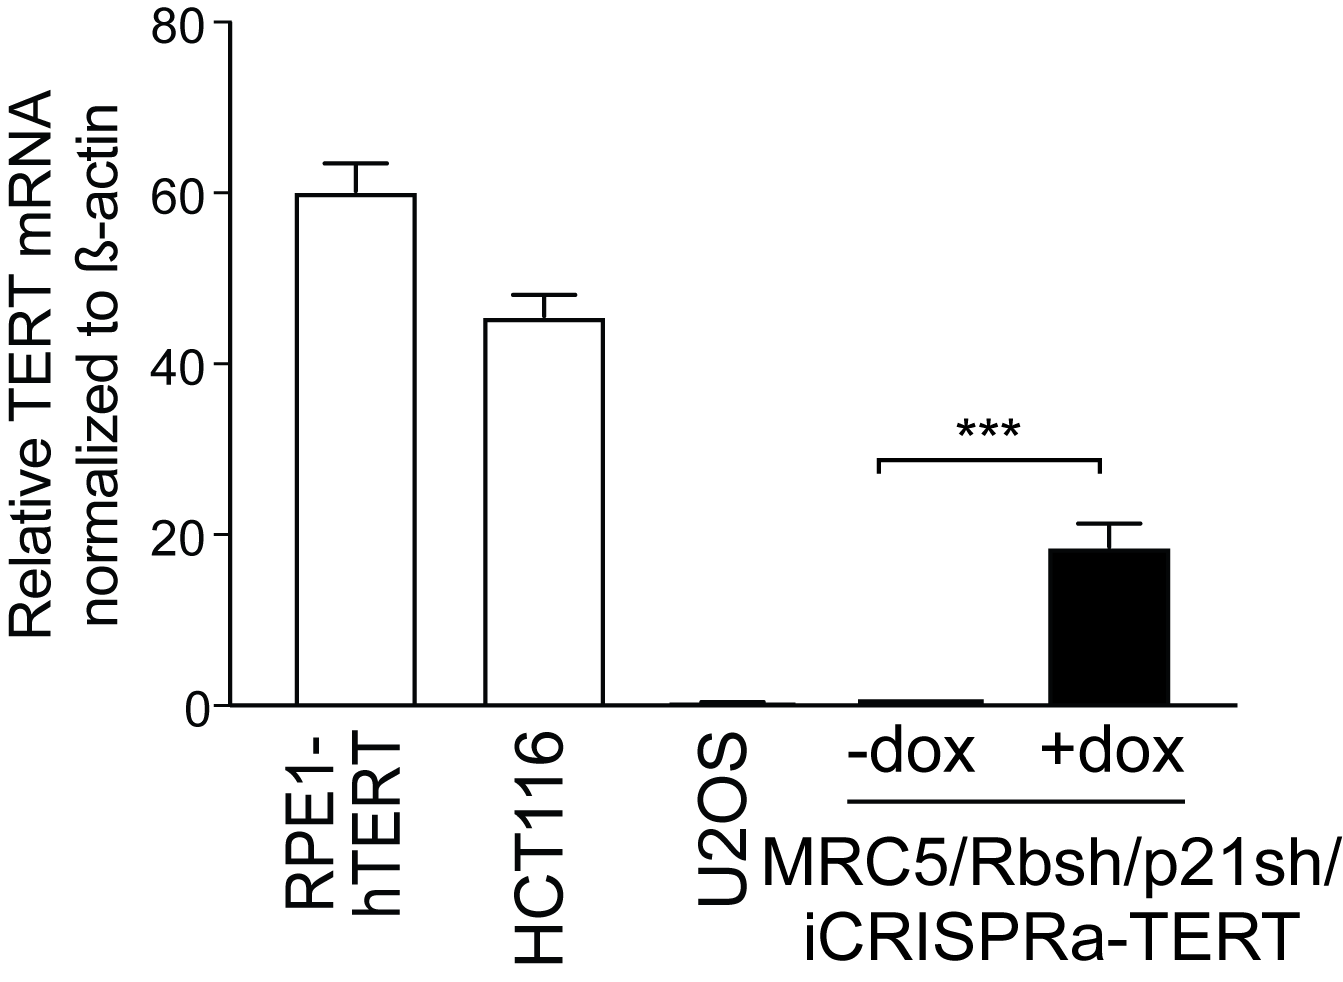
\includegraphics[width=0.95\linewidth]{figures/600ppi/tc_tert_qpcr.png}
    \caption{\textbf{Expression of TERT mRNA after doxycycline induction.}}
    \label{fig:tc_tert_qpcr}
\end{figure}

\begin{figure}
    \centering
    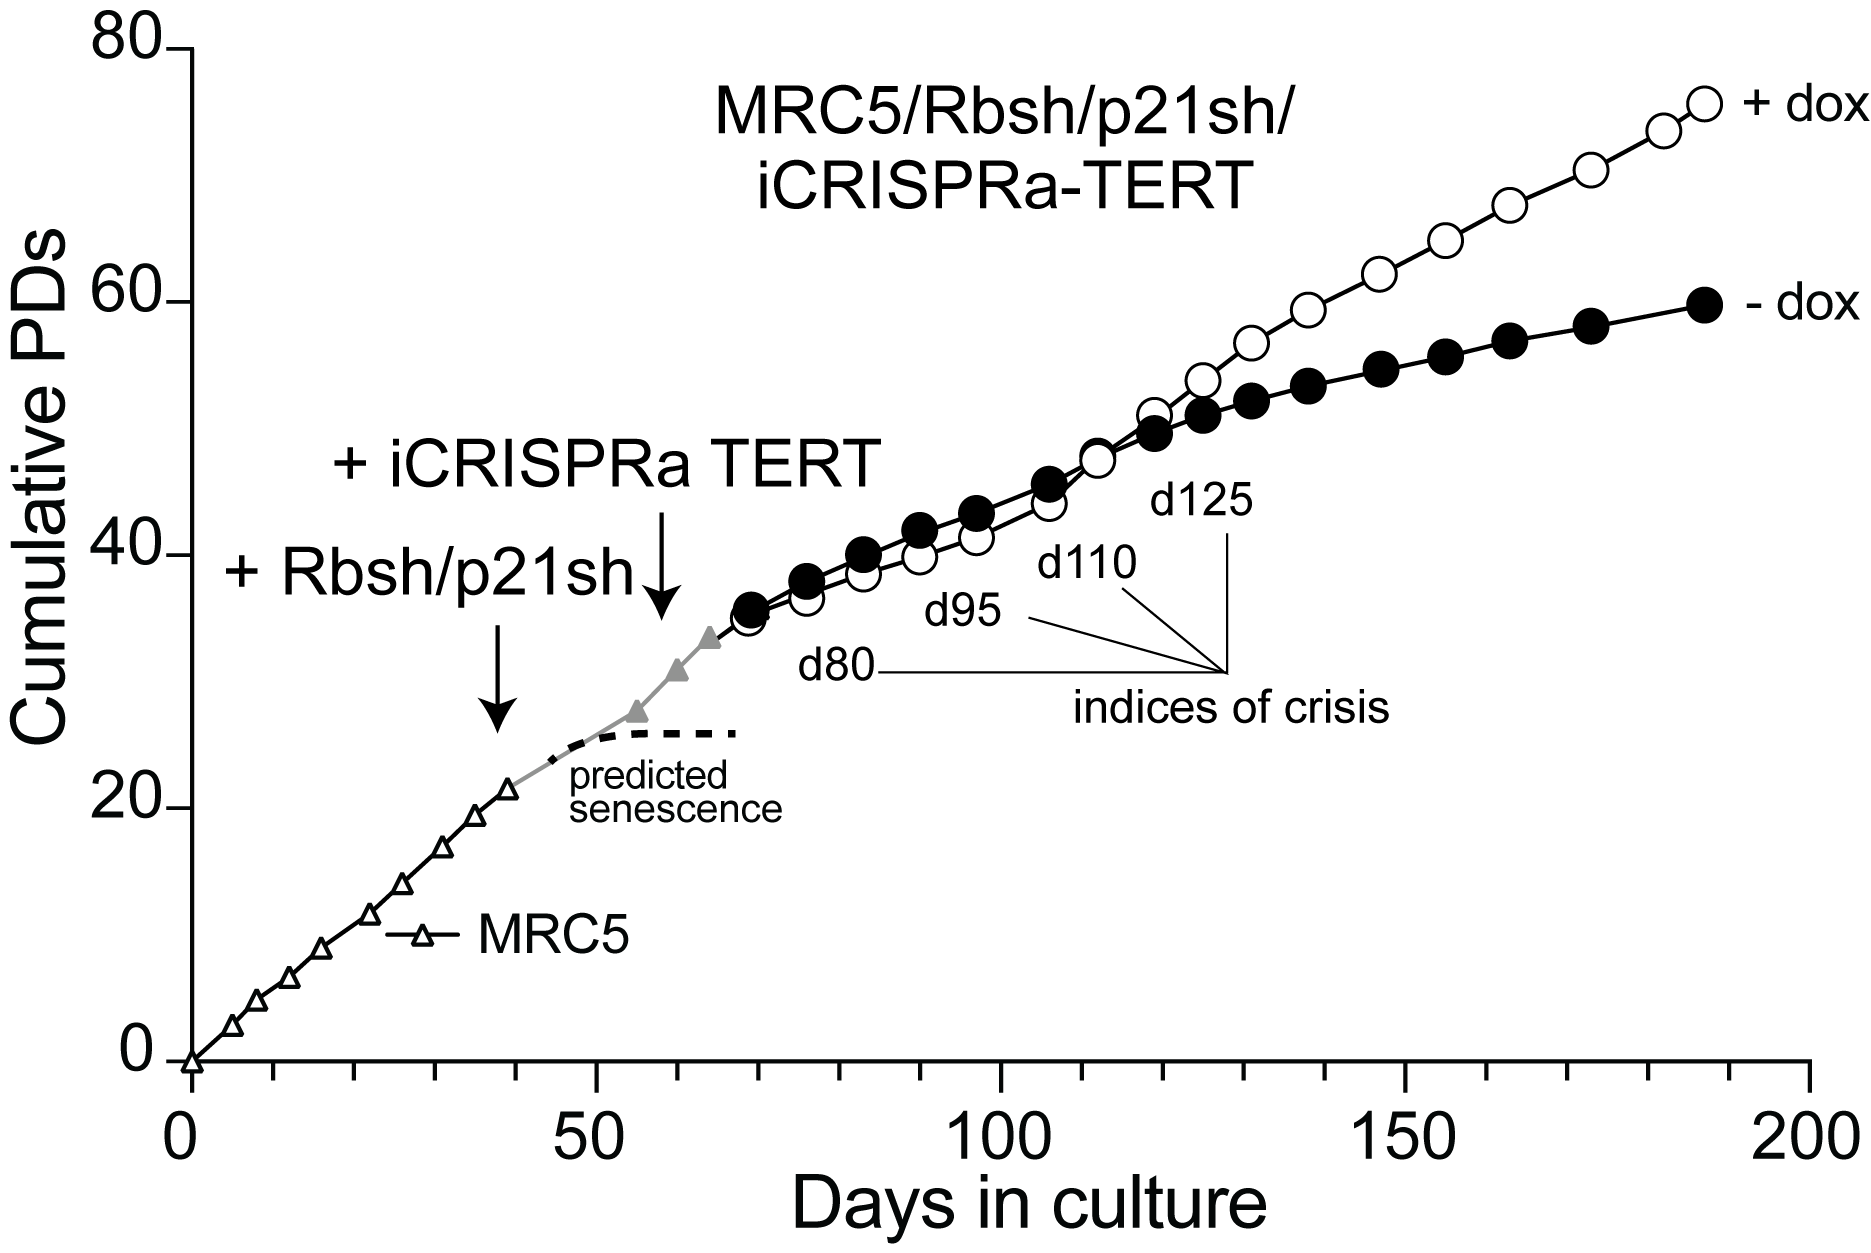
\includegraphics[width=0.95\linewidth]{figures/600ppi/tc_growth_original.png}
    \caption{\textbf{Population doubling in induced versus control group over time.}}
    \label{fig:tc_growth_original}
\end{figure}

To gain a clearer insight into the nature of SVs that arise during telomere crisis, we developed an in vitro system in which we could reproduce telomere crisis and generate a large number of post-crisis clones. MRC5 human lung fibroblasts were chosen to model telomere crisis since they lack telomerase activity and as a consequence have a well-defined in vitro replicative potential determined by telomere attrition. To bypass senescence, the Rb and p21 pathways were inactivated by infecting the population of MRC5 cells with a retrovirus bearing shRNAs targeting the respective transcripts (data not included, refer to \cite{Dewhurst2021-jk} Supplementary Figure 2A). This population of MRC5/Rbsh/p21sh was then endowed with an inducible CRISPR activation system (iCRISPRa) to activate the TERT promoter and induce telomerase expression (Figure \ref{fig:tc_system}). The iCRISPRa system employed a doxycycline-inducible nuclease-dead Cas9 fused to a tripartite transcriptional activator (VP64-p65-Rta) \cite{Chavez2015-md} and four gRNAs targeting the TERT promoter (Figure \ref{fig:tc_tert_western}, \ref{fig:tc_system}). Addition of doxycycline (dox) to MRC5/Rbsh/p21sh/iCRISPRa-TERT cells resulted in induction of TERT mRNA within 96 hours, whereas without dox, TERT transcripts are undetectable in this cell line (p<0.001, Figure \ref{fig:tc_tert_qpcr}). A similar dox-induced increase in mRNA expression was noted upon introduction of sgRNAs to a control gene (data not included, refer to \cite{Dewhurst2021-jk} Supplementary Figure 2C). Induction of telomerase activity was readily detectable in a TRAP (telomerase repeated amplification protocol) assay (data not included, refer to \cite{Dewhurst2021-jk} Figure 2C). However, the induced TERT mRNA levels and the TRAP activity were significantly lower than in telomerase-positive control cell lines. The relatively weak telomerase activity in this system harmonizes with recent work showing that cancer-associated TERT promoter mutations initially result in low levels of telomerase activity that is not sufficient to maintain bulk telomere length \cite{Chiba2017-gq}.

\begin{figure}
    \centering
    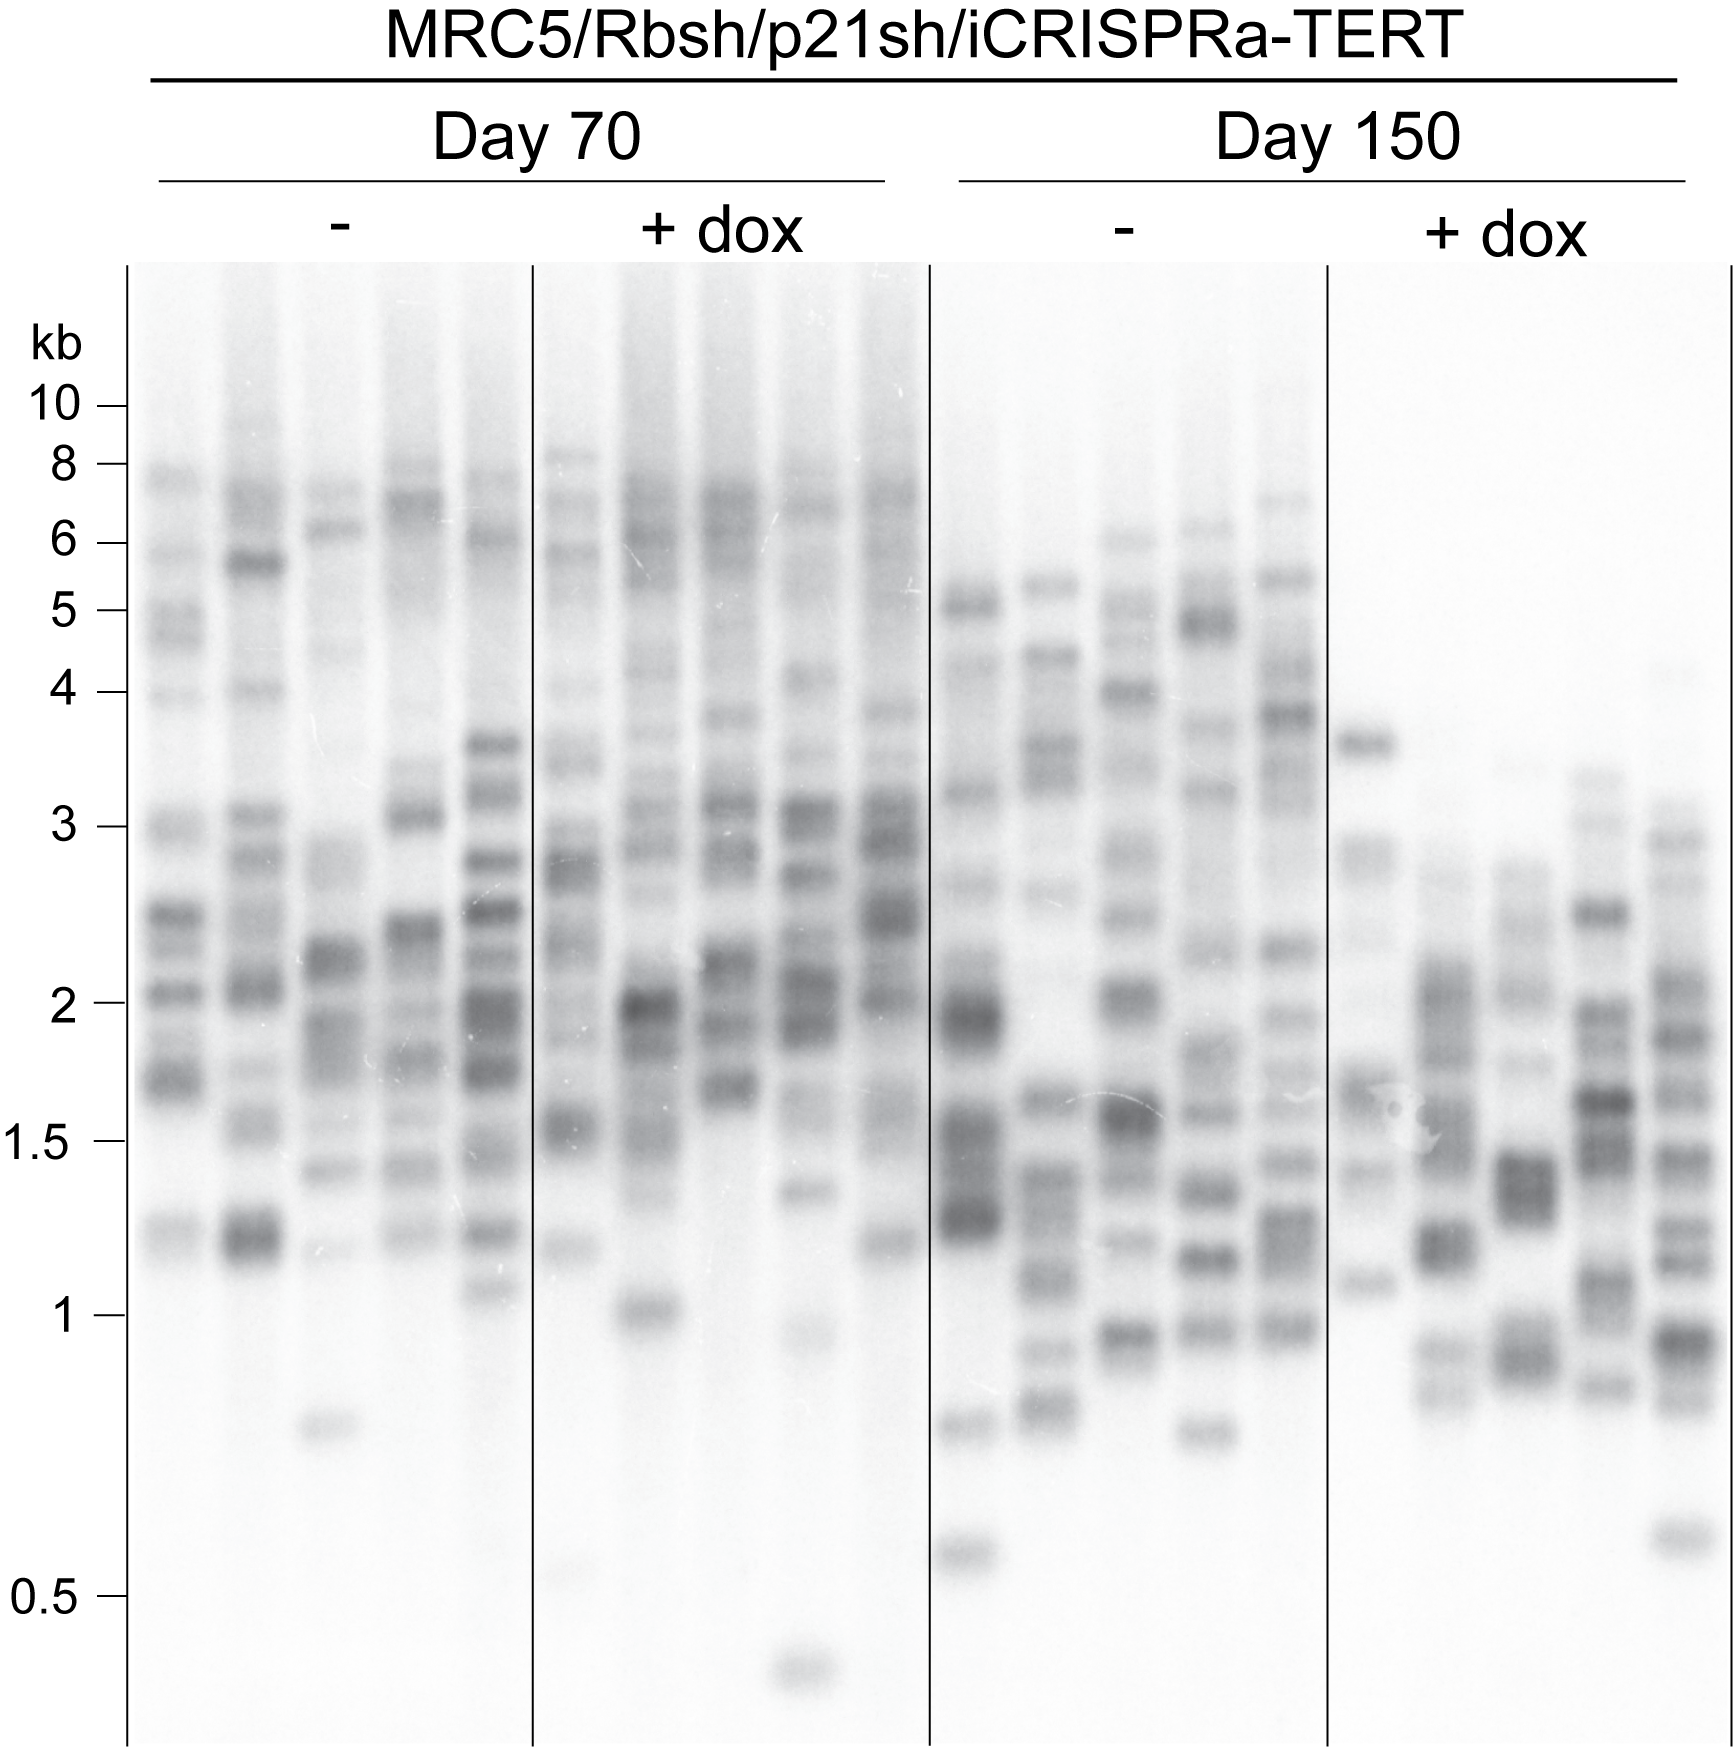
\includegraphics{figures/600ppi/tc_stela.png}
    \caption{\textbf{STELA of XpYp telomeres in MRC5/Rbsh/p21sh/iCRISPRa-TERT cells with or without doxycycline treatment at 70 and 150 days of culture.}}{}
    \label{fig:tc_stela}
\end{figure}

At approximately 120 days after the start of the experiment (55 days with dox) the MRC5/Rbsh/p21sh/iCRISPRa-TERT population was proliferating faster than their untreated counterparts (Figure \ref{fig:tc_growth_original}). Inspection of individual telomere lengths using Single Telomere Length Analysis (STELA, \cite{Baird2003-cj}) revealed that although telomerase expression was sufficient to allow the cells to proliferate, it was not sufficient to maintain bulk telomere length (Figure \ref{fig:tc_stela}). After 150 days of continuous culture, the majority (86\%) of XpYp telomeres in induced MRC5/Rbsh/p21sh/iCRISPRa-TERT cells were between 1-4 kb compared to 40\% in uninduced cells (data not included, refer to \cite{Dewhurst2021-jk} Figure 2F, Supplementary Figure 2D). Consistent with this, genomic blotting showed bulk telomere shortening in both induced and uninduced cells (data not included, refer to \cite{Dewhurst2021-jk} Figure 2G). These telomere dynamics are consistent with the expectation that in the culture without telomerase, cells with critically short telomeres will preferentially be lost, leading to a surviving population with relatively longer telomeres. In contrast, cells in the induced culture with (low) telomerase activity have the ability to elongate the shortest telomeres. As a result, the induced cells are expected to tolerate telomere attrition better and present with overall shorter telomeres at later time points.

\section{Genomic screening of post-crisis clones}
\begin{figure}
    \centering
    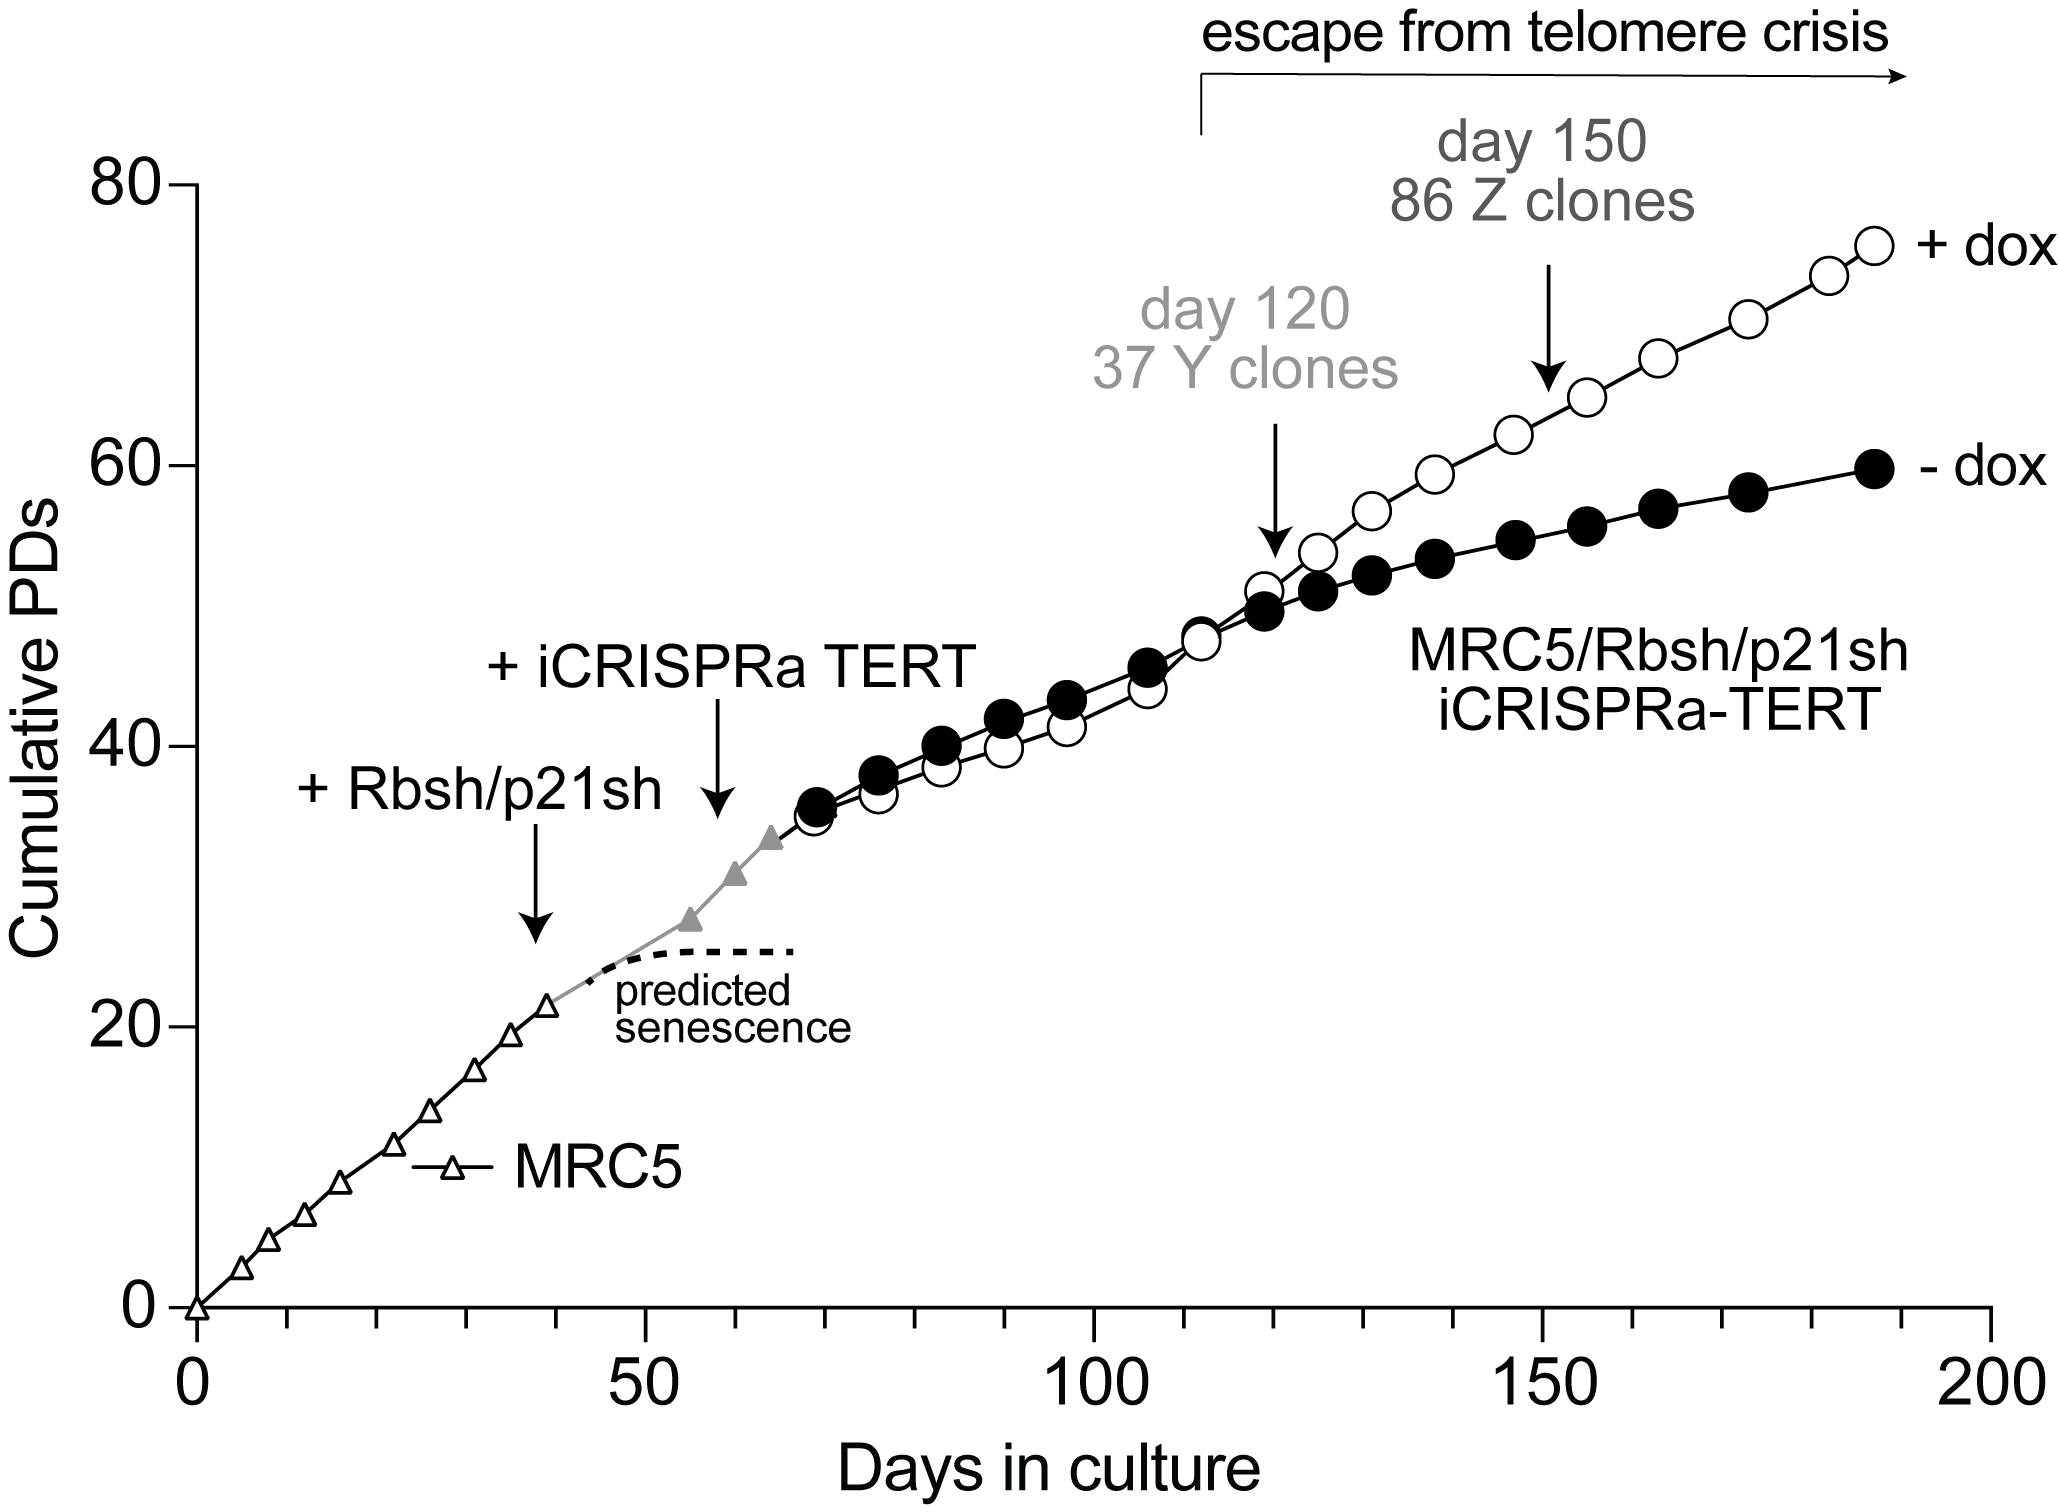
\includegraphics[width=0.95\linewidth]{figures/600ppi/tc_growth.png}
    \caption{\textbf{Clones are isolated at day 120 and day 150 for whole genome sequencing.}}
    \label{fig:tc_growth}
\end{figure}

\begin{figure}
    \centering
    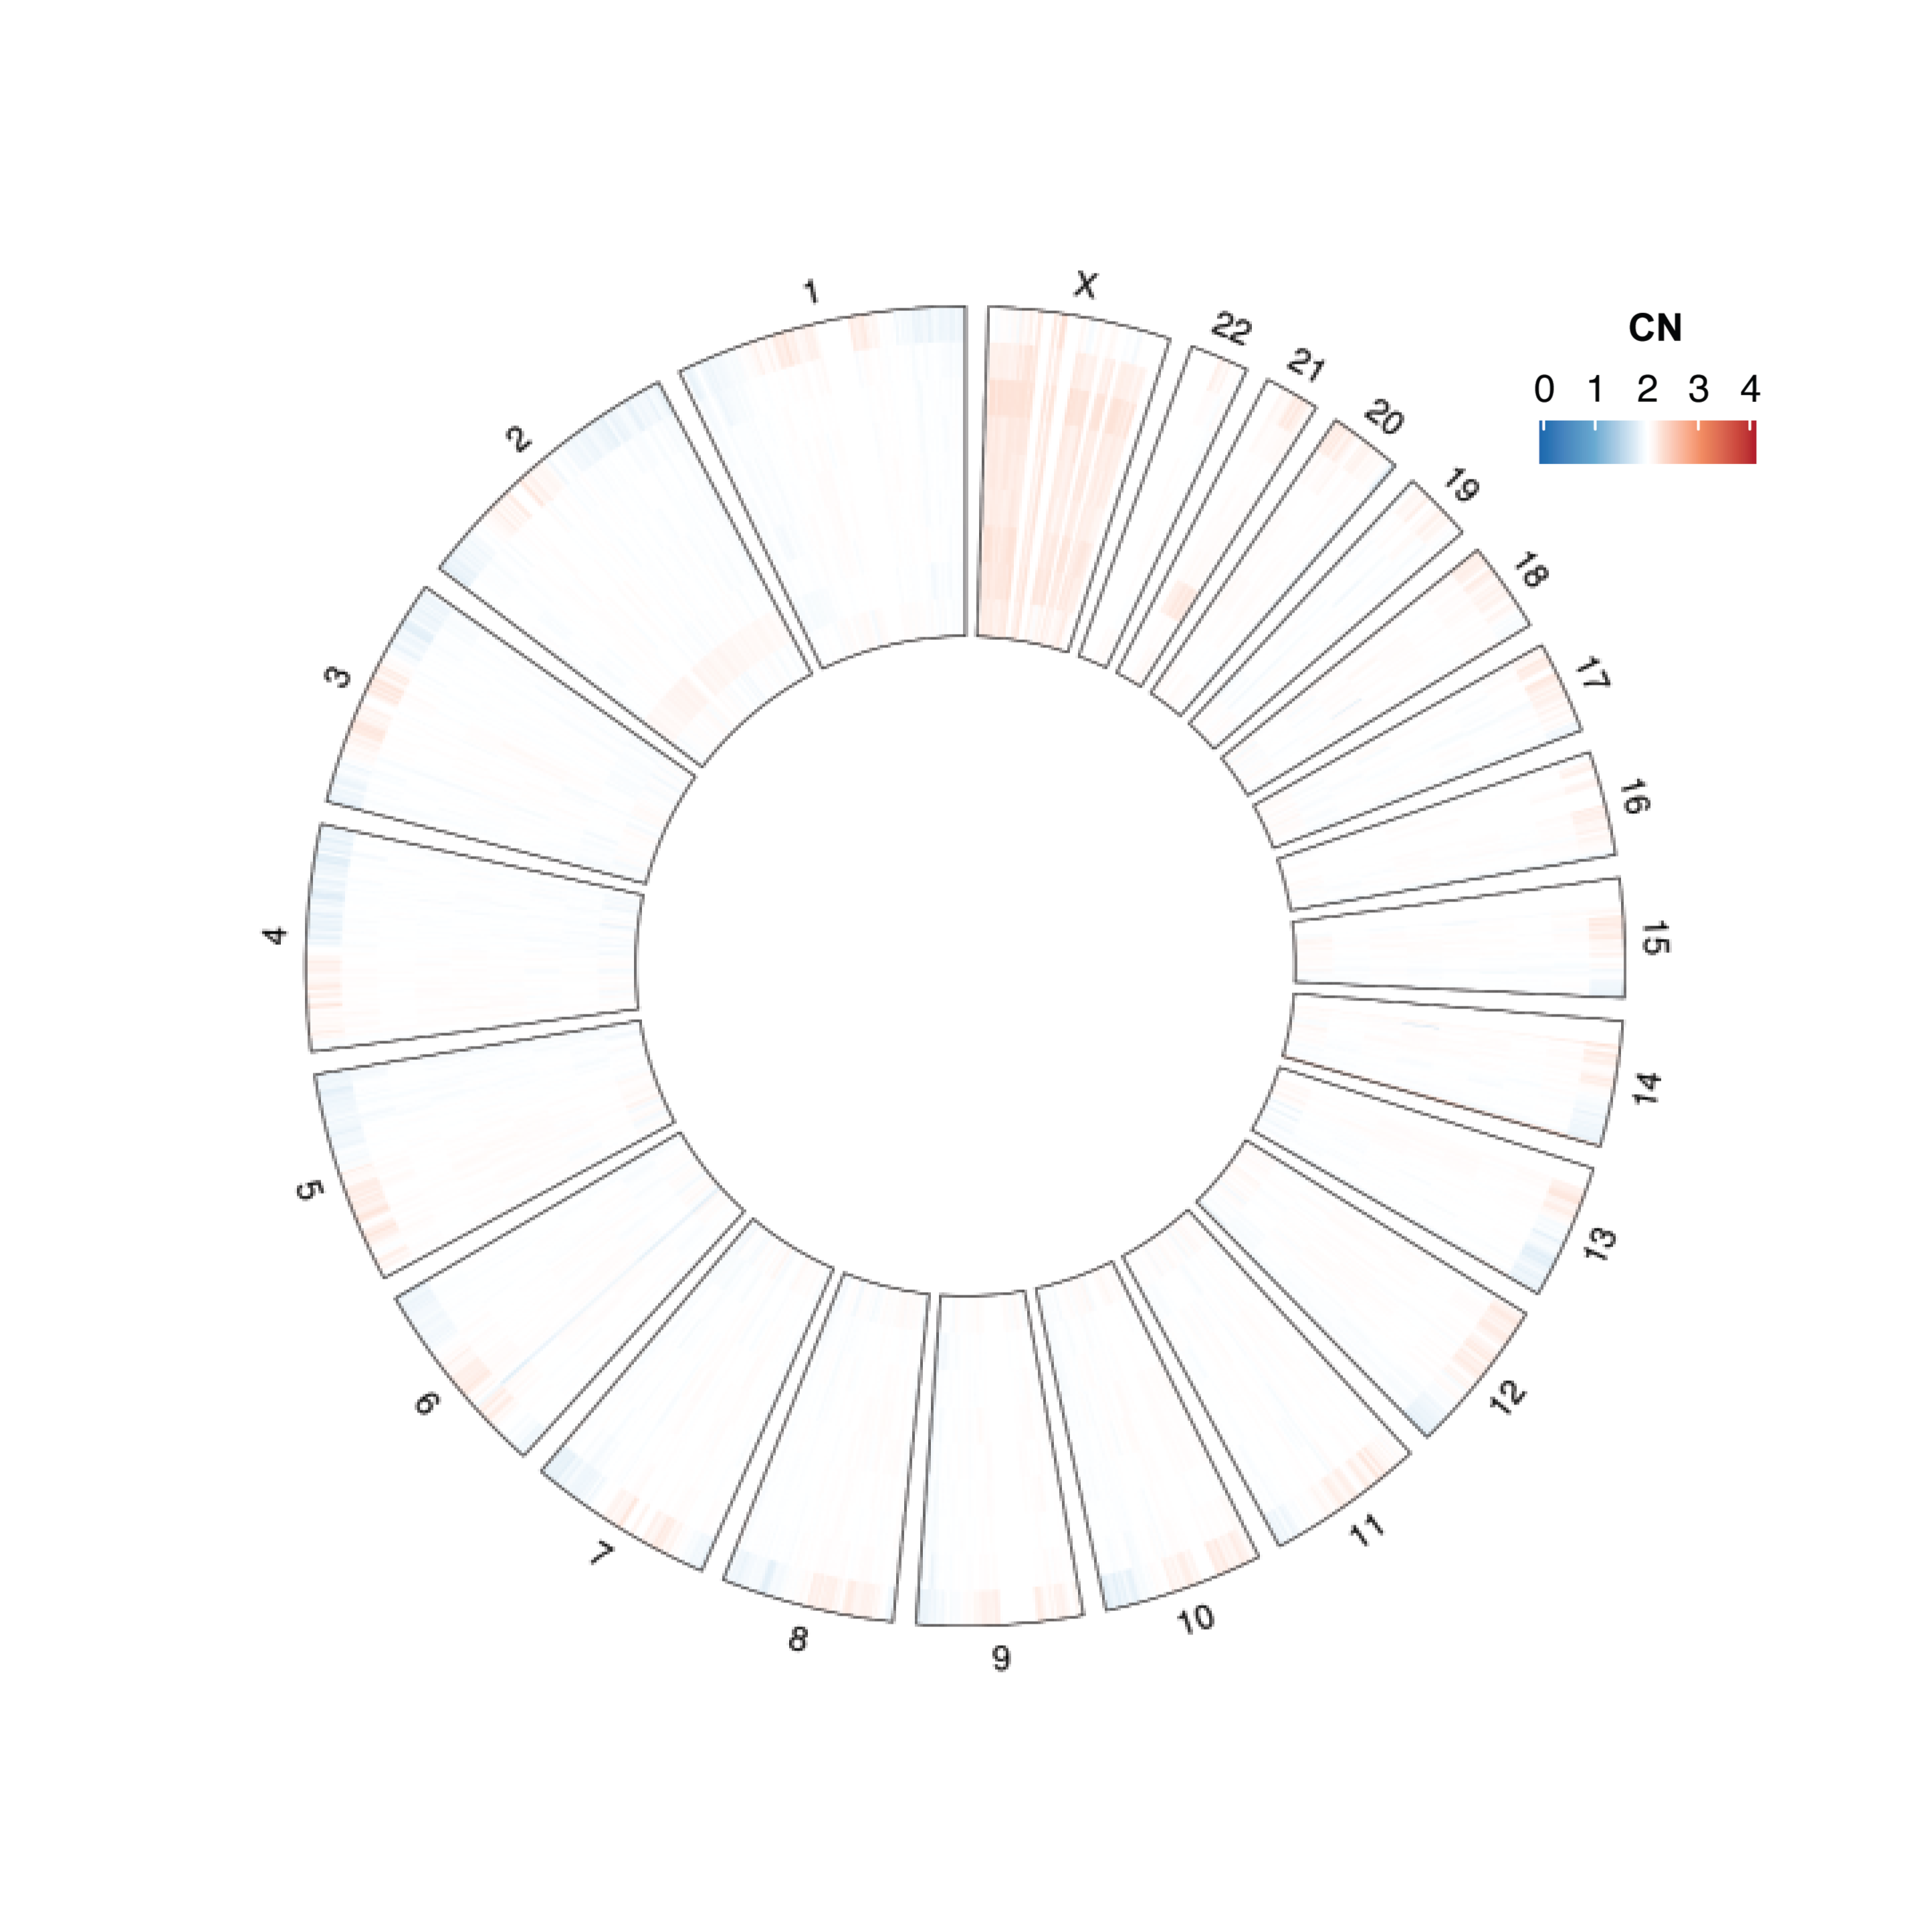
\includegraphics[width=0.95\linewidth]{figures/600ppi/tc_heatmap_tert_control.png}
    \caption{\textbf{Control group with exogeneous TERT show no CNA.}}
    \label{fig:tc_heatmap_tert_control}
\end{figure}

\begin{figure}
    \centering
    \includegraphics[width=0.95\linewidth]{figures/600ppi/tc_sum_coverage_low.png}
    \caption{\textbf{Aggregated coverage of the putative BFB clones.}}
    \label{fig:tc_sum_coverage_low}
\end{figure}

\begin{table}[h!]
\label{tab:tc_sequenced_clones}
\begin{tabular}{ccc}
\hline
\multirow{0}{0pt}{Name} & \multicolumn{2}{c}{\textbf{Number   Sequenced}} \\ \cline{2-3} 
                      & Low Pass         & High   Pass         \\ \hline
Parental cell lines   & 3                & 1                   \\
Day 120 (Y) clones    & 37               & 5                   \\
Day 150 (Z) clones    & 83               & 8                   \\
Control (CT) clones   & 8                & 0                   \\ \hline
\end{tabular}
\caption{Number of clones analyzed by high and low-pass WGS}
\end{table}

\begin{table}[] \label{tab:tc_sv40t}
\rotatebox[]{90}{
    \begin{tabular}{ccccc}
        \hline
        \textbf{Name}                  & \textbf{Cell Line/Tissue Source}              & \textbf{Telomerase Status}   & \textbf{Reference}                 & \textbf{Kind gift of}             \\ \hline
        HA1 p15               & Human Embryonic   Kidney cells       & -            & \cite{Counter1992-yg}  & Silvia   Bacchetti/AdVec \\
        SW13 PD73             & IMR90 lung   fibroblasts             & -            & \cite{Shay1989-ua} & Jerry Shay, UTSW         \\
        SW26 PD68.5           & IMR90 lung   fibroblasts             & -            & \cite{Shay1989-ua} & Jerry Shay, UTSW         \\
        SW39 PD72.5           & IMR90 lung   fibroblasts             & -            & \cite{Shay1989-ua} & Jerry Shay, UTSW         \\
        Bet3B p3              & NHBE-10 bronchial   epithelial cells & -            & \cite{Bryan1995-ik}     & Roger Reddel, CMRI       \\
        Bet3K p7              & NHBE-10 bronchial   epithelial cells & -            & \cite{Bryan1995-ik}  & Roger Reddel, CMRI       \\
        BFT3B p10             & BF-10 bronchial   fibroblasts        & -            & \cite{Bryan1995-ik}    & Roger Reddel, CMRI       \\
        BFT3G p7              & BF-10 bronchial   fibroblasts        & -            & \cite{Bryan1995-ik}  & Roger Reddel, CMRI       \\
        BFT3K p9              & BF-10 bronchial   fibroblasts        & -            & \cite{Bryan1995-ik}    & Roger Reddel, CMRI       \\
        HA1-IM PD216          & Human Embryonic   Kidney cells       & + & \cite{Counter1992-yg}  & Silvia   Bacchetti/AdVec \\
        SW13 PD184            & IMR90 lung   fibroblasts             & +  & \cite{Shay1989-ua} & Jerry Shay, UTSW         \\
        SW26 PD130+           & IMR90 lung   fibroblasts             & +  & \cite{Shay1989-ua} & Jerry Shay, UTSW         \\
        SW39 PD130+           & IMR90 lung   fibroblasts             & +  & \cite{Shay1989-ua} & Jerry Shay, UTSW         \\
        Bet3B p25 post-crisis & NHBE-10 bronchial   epithelial cells & + & \cite{Bryan1995-ik}      & Roger Reddel, CMRI       \\
        Bet3K p25 post-crisis & NHBE-10 bronchial   epithelial cells & + & \cite{Bryan1995-ik}      & Roger Reddel, CMRI       \\
        BFT3B p28 post-crisis & BF-10 bronchial   fibroblasts        & + & \cite{Bryan1995-ik}      & Roger Reddel, CMRI       \\
        BFT3G p28 post-crisis & BF-10 bronchial   fibroblasts        & + & \cite{Bryan1995-ik}      & Roger Reddel, CMRI       \\
        BFT3K p34 post-crisis & BF-10 bronchial   fibroblasts        & + & \cite{Bryan1995-ik}      & Roger Reddel, CMRI       \\ \hline
    \end{tabular}
}
\caption{\textbf{SV40T immortalized pre-crisis and post-crisis telomerase positive cell lines.}}
\end{table}

To assess the genome structure of proliferating post-crisis cells, single cell clones were isolated from induced MRC5/Rbsh/p21sh/iCRISPRa-TERT cells at day 120 (‘Y clones’) and day 150 (‘Z clones’) (Figure \ref{fig:tc_growth}). The clonal yield at day 150 was greater than at day 120 in induced cells but no clones could be isolated from the uninduced population at either timepoint. The lower clonal yield at day 120 may be due to incomplete stabilization of the telomeres since clones from this time-point showed a higher burden of fused telomeres than those derived from day 150 (data not included, refer to \cite{Dewhurst2021-jk} Supplementary Figure 4A). Post-crisis clones from both timepoints showed evidence of ultra-short telomeres and reduced telomere length (data not included, refer to \cite{Dewhurst2021-jk} Supplementary Figure 4B-C). Telomerase activity in post-crisis clones was comparable to the parental induced population, indicating that clone viability was not due to selection for increased telomerase activity (data not included, refer to \cite{Dewhurst2021-jk} Supplementary Figure 4D). To generate control clones which had not passed through a period of telomere crisis, early passage MRC5 cells were infected with a retrovirus expressing hTERT and single cell clones were isolated (data not included, refer to \cite{Dewhurst2021-jk} Supplementary Figure 4E). Genome profiling with low pass (~5X) WGS was performed on eight hTERT-expressing control clones (CT clones), 36 Y clones from day 120, and 82 Z clones from day 150 (Table \ref{tab:tc_sequenced_clones}).

\begin{figure}[h!]
    \centering
    \includegraphics[width=0.95\linewidth]{figures/600ppi/tc_circos_low.png}
    \caption{\textbf{Circular heatmap showing genome-wide binned purity- and ploidy-transformed read depth.}}{Units are CN across 118 low-pass WGS-profiled clones. Heatmap rows correspond to concentric rings in the heatmap. Clones are clustered with respect to genome-wide copy number profile similarity (see “Methods”).}
    \label{fig:tc_circos_low}
\end{figure}

\begin{figure}[h!]
    \centering
    \includegraphics[width=0.95\linewidth]{figures/600ppi/tc_heatmap_low.png}
    \caption{\textbf{Post-crisis clones are clustered into six groups based on CN profile of chromosome 12 and 21.}}
    \label{fig:tc_heatmap_low}
\end{figure}

Analysis of genome-wide read depth across 118 clones from both day 120 (Y clones) and day 150 (Z clones) demonstrated predominantly diploid genomes with a striking enrichment of clones with DNA loss on most of chromosome 12p (63\%, 74/118, Figure \ref{fig:tc_circos_low}). Within the other 44 samples, we observed a subset of clones (5\%, 6/118, Figure \ref{fig:tc_circos_low}) with gains of chromosome 21q. As expected, control CT clones showed no evidence of SVs or copy number variants (Figure \ref{fig:tc_heatmap_tert_control}). Hierarchical clustering of all clones by their coverage on chromosomes 12p and 21q revealed six distinct clusters (Figure \ref{fig:tc_heatmap_low}). A minority of clones were diploid on chromosomes 12 and 21 and elsewhere in the genome and are therefore designated as ‘unrearranged’ (32\% of clones, 38/118). Of note, the unrearranged group was enriched in day 120 (Y) samples compared to day 150 (Z) samples (p = 1.79x10-9, odds ratio 14.7, Fisher’s exact test; Figure \ref{fig:tc_heatmap_low}), suggesting that these clones may have largely avoided crisis prior to telomerase induction. The cluster of clones with 21q gain were diploid on 12p.

The remaining 74 clones (63\%) all showed a heterogenous pattern of copy number alterations targeting 12p (Figure \ref{fig:tc_heatmap_low}). One out of the 118 clones (0.8\%) displayed the singular pattern of distinct interspersed losses that resembled chromothripsis. Complete loss of one copy of 12p ('arm loss') was found in a cluster of 6 clones (6/118, 5\%). A second cluster of 67 clones all shared a breakpoint near the distal end of 12p and a large deletion starting ~9 Mbp from the centromere. These clones were differentiated into two clusters by the presence or absence of an amplification around 8-9 Mbp from the 12p telomere. In the 47 clones that contained this amplification, aggregated consensus read depth profiles revealed stepwise gains at the distal end of 12p, a pattern reminiscent of BFB cycles (Supplementary Figure \ref{fig:tc_sum_coverage_low}). This cluster was therefore labelled ‘BFB-like’, a designation which is further supported by data presented below. The 20 clones (17\%) that lack the amplicon around 8-9 Mbp harbored varying boundaries of the shared larger deletion; based on the analysis described below we designate these as ‘early BFB-like’. In summary, these low-pass WGS copy number profiles indicated a limited set of distinct lineages surviving telomere crisis, with at least two lineages independently converging on 12p.

% insert the formulation of multisample graph fitting -- walk decomposition
\section{Joint inference of junction balance in MRC5} \label{sec:joint_jabba_mrc5}
To chart structural variant evolution across sub-clades of MRC5 clones, a procedure was developed to jointly infer junction balanced genome graphs in a lineage (e.g. BFB lineage in Figure 5C). This co-calling algorithm augmented the existing JaBbA model, described in detail in \cite{Hadi2020-um}, enabling application to a compendium of genome graphs by minimizing the total number of unique loose ends assigned a nonzero copy number across the graph compendium.  

Formally, we define a collection ${G^i = (V^i, E^i)}, i \in 1,\dots,n$ of identical genome graphs across $n$ clones, each a replica of a \textit{prototype} genome graph $G^0 = (V^0, E^0)$. The mapping $p:V \cup E \rightarrow V^0 \cup E^0$ maps each vertex $v \in V^i$ and edge $e \in E^i,i \in 1,\dots,n$ to its corresponding vertex $p(v)\in V^0$ and edge $p(e) \in E^0$ in the prototype graph. We then jointly infer unique copy number assignments $\kappa^i$ to the vertices and edges of each genome graph $G^i$ by solving the mixed integer program:

\begin{equation} \label{eq:multi_sample_jabba}
    \begin{aligned}
        \underset{\kappa^i:V_I(G^i) \cup E(G^i) \rightarrow \mathbb{N}, i \in 1,\dots,n}{\text{minimize}} &
        \lambda \mathcal{R}(\{G^i\}_{i \in 0, \dots, n}, \{\kappa^i\}_{i \in 1, \dots, n}, p) + \sum_{i \in 1,\dots,n}\mathcal{V}(G^i, \kappa^i, x^i, J^i) \\
        \text{subject to: } & \kappa^i(v) = \kappa^i(\bar{v}), \forall_{v \in V_I^i} \\
        & \kappa^i(e) = \kappa^i(\bar{e}), \forall_{e \in E^i} \\
        & \kappa^i(v) = \sum_{e \in E^+(v,G^i)}\kappa^i(e) = \sum_{e \in E^-(v, G^i)}\kappa^i(e) \\
        & \kappa^i(e) \le u^i(e)
    \end{aligned}
\end{equation}

where $x^i$ and $J^i$ represent the binned read depth data and bin-node mappings for clone $i$ and  $\mathcal{V}(G^i,κ^i,x^i,J^i)$ is the read depth residual for genome graph i, analogous to \ref{eq:MIQP}.  A new term in this joint formulation is $u^i:E(G^i) \rightarrow \{0,\inf\}$, which is a constraint on the upper bound of each edge CN $\kappa(e) \in E(G^i)$, e.g. zero if there have been no read support for the junction in clone $i$. 

The coupling of multiple graphs happen through a joint complexity penalty $\mathcal{R}$, which only penalize a loose end once for all the clones. Formally,

\begin{equation} \label{eq:joint_loose_penalty}
    \mathcal{R}(\{G^i\}_{i \in 0, \dots, n}, \{\kappa^i\}_{i \in 1, \dots, n}, p) = \sum_{v \in V(G^0)}[\![ \sum_{\hat{v}|\hat{v} \in G^i, p(\hat{v})=v, i \in 1,\dots,n} \kappa^i(\hat{v}) ]\!]
\end{equation}

As in \ref{eq:MIQP}, the hyperparameter $\lambda$ in Equation \ref{eq:multi_sample_jabba} controls the relative contribution of the read-depth residual and complexity penalty to the objective function. 

It is important to note that while each of the graphs $G^i$ have an identical structure, the constraints imposed by the upper bounds $u^i$ and bin profiles $x^i$ confine each graph to its junctions and read depth data, and hence lead to a unique fit $κ^i$ on the basis of this data. The $L_0$ penalty (defined using the Iversion bracket $[\![]\!]$ operator) in Equation \ref{eq:joint_loose_penalty} couples the solutions $κ^i$ by adding an exponential prior on the number of unique loose ends across the entire graph compendium, where uniqueness is defined by the mapping $p$ to the prototype graph $G^0$.

This joint mixed-integer programming model in Equation \ref{eq:multi_sample_jabba} is implemented in the “balance” function of gGnome. The model was applied to a collection of genome graphs representing the structure of chromosome 12 across 13 clones. The prototype graph for this genome graph collection was built from the disjoint union of intervals of the 13 preliminary graphs (via the GenomicRanges “disjoin” function) and the union of junction calls fit across those graphs (via gGnome “merge.Junction” function). Each graph was associated using the read depth data and bin-to-node mappings as per \cite{Hadi2020-um}. The mapping $u^i$ for each reference edge was set to $\inf$ while variant edges were assigned $\inf$ if bwa mem realignments of read pairs in each clone .bam file to the corresponding junction contig via rSeqLib (https://github.com/mskilab/rSeqLib, \cite{Wala2017-ud}), otherwise they were assigned 0.

Equation \ref{eq:multi_sample_jabba} was then solved using the IBM CPLEX (v12.6.2) MIQP optimizer within the gGnome package after setting the hyperparameter $\lambda$ to 100.  This value was chosen after a parameter sweep observing for the visual concordance of genome graphs, loose ends, and read depth profiles in the region.

\section{High-resolution reconstruction and lineage of post-crisis genomes} \label{sec:tc_joint_decomposition}
\begin{figure}
    \centering
    \includegraphics[width=0.95\linewidth]{figures/600ppi/tc_evo_tree.png}
    \caption{\textbf{Evolutionary trajectory of SVs in clones with high-pass WGS.}}
    \label{fig:tc_evo_tree}
\end{figure}

\begin{figure}
    \centering
    \includegraphics[width=0.95\linewidth]{figures/600ppi/tc_phylo.png}
    \caption{\textbf{Phylogenetic tree reconstructed based on SNVs.}}
    \label{fig:tc_phylo}
\end{figure}

\begin{figure}
    \centering
    \includegraphics[width=0.95\linewidth]{figures/600ppi/tc_kataegis.png}
    \caption{\textbf{Clustered SNVs around junction breakends.}}
    \label{fig:tc_kataegis}
\end{figure}

\begin{figure}
    \centering
    \includegraphics[width=0.95\linewidth]{figures/600ppi/tc_12q_del.png}
    \caption{\textbf{Simple deletion on chromosome 12q present in Y15, Y8, Z43, but not Y11.}}
    \label{fig:tc_12q_del}
\end{figure}

\begin{figure}
    \centering
    \includegraphics[width=0.95\linewidth]{figures/600ppi/tc_loose_end.png}
    \caption{\textbf{Distinct loose ends among the diverging BFB clones.}}
    \label{fig:tc_loose_end}
\end{figure}

To gain further insight into structural variant evolution along these lineages, we chose 15 representative clones spanning the 5 clusters with rearrangements involving 12p for high-depth WGS to a median read depth of 50X (range: 30-88). Phylogenies derived from genome-wide SNV patterns demonstrated a median branch length of 551 SNVs (range: 9-2,409), a low mutation density (<1 SNV/Mbp) that is consistent with previous WGS studies of clones in cell culture \cite{Petljak2019-cf}. This analysis revealed four major clades (Figure \ref{fig:tc_phylo}). These clades had good concordance with copy number alteration and rearrangement junction patterns in the same 12p region, suggesting these clones represent distinct post-crisis evolutionary lineages (Figure \ref{fig:tc_phylo}).

In order to further reconcile the shared and distinct rearrangement junctions present in the evolution of these clones, we carried out local assembly of rearrangement junctions and junction balance analysis (see \ref{sec:tc_joint_jabba}) which revealed 7 distinct junction-balanced genome graphs spanning 12p (Figure \ref{fig:tc_evo_tree}). With the exception of the chromothriptic lineage (see below), each of these distinct lineages was represented by more than one post-crisis clone.

To reconstruct a set of linear alleles that parsimoniously explain these different genome graph patterns3 (Figure \ref{fig:tc_evo_tree}), we applied gGnome to the data (see \nameref{sec:tc_joint_decomposition}). We constrained our model to contain one intact allele of chromosome 12 for the following reasons: 1) karyotypes and chromosome painting showed a single copy of chromosome 12 was altered in the post-crisis clones (Figure \ref{fig:tc_fish_bicolor}, \ref{fig:tc_fish_bicolor_all}); and 2) rearrangement of one allele is more likely than rearrangement across two alleles. Application of this constraint to the full set of MRC5 clones in a joint inference revealed a parsimonious set of rearranged alleles that explained the observed collection of clonally-related junction-balanced graphs (Figure \ref{fig:tc_evo_tree}).

\section{Joint reconstruction of allelic evolution in MRC5} \label{sec:tc_joint_jabba}
Evolving 12p alleles were jointly reconstructed across 13 MRC5 clones through the decomposition of junction balanced genome graphs $(G^i,κ^i)$ (see \nameref{sec:joint_jabba_mrc5} section above). The procedure for joint allelic phasing described in \cite{Hadi2020-um} and \nameref{eq:walk_decomposition} was extended to identify the most parsimonious (least unique walks needed) collection of paths and/or cycles $H$ and associated walk multiplicity $\kappa(H)$ that summed to the vertex and edge copy numbers in the compendium $(G^i,κ^i)$.

Formally, the subgraph of vertices and edges with a nonzero copy number in each $(G^i,κ^i)$ were exhaustively traversed to derive all minimal paths and cycles $H^i$, where for each walk $h \in H^i$ maps to incident sequences of $V(h) \subseteq V^i$ and $E(h) \subseteq E^i$ of vertices and edges in the graph $G^i$.  The nodes and vertices of these walks were then projected to via the mapping $p$ to define a unique set of walks $H^0$ in the prototype graph $G^0$. We extend our notation $p$ (see previous section) so that for a walk $h \in H^i$ the mapping $p(h) \in H^0$ denotes the walk formed by projecting the vertices and edges of $h$ via $p$ to $H^0$.  With these definitions, the single graph haplotype inference defined in \ref{eq:walk_decomposition} was extended to a joint inference by solving the following mixed integer linear program to assign a copy number $\kappa^i(h) \in \mathbb{N}$ to each walk $h \in H^i$:

\begin{equation} \label{eq:joint_walk_decomposition}
    \begin{aligned}
        \underset{\kappa^i(h):H^i \rightarrow \mathbb{N}, i \in 1, \dots, n}{\text{minimize}} & \sum_{h \in H^0} [\![ \sum_{\hat{h} \in H^i | p(\hat{h} = h)} \kappa^i(h) ]\!] \\
        \text{s.t. } & \kappa^i(v) = \sum_{h \in H^i} \kappa(h)\delta(h, v), \forall v \in V^i, i \in 1, \dots, n \\
        & \kappa^i(e) = \sum_{h \in H^i} \kappa(h)\delta(h, e), \forall e \in E^i, i \in 1, \dots, n
    \end{aligned}
\end{equation}

where the function $\delta(v,h)$ and $\delta(e,h)$ is 1 if vertex $v$ and edge $e$ belong to walk $h$ and 0 otherwise, just like in \ref{eq:walk_decomposition}. The Iverson bracket ($[\![]\!]$) operator in the objective function Equation \ref{eq:joint_walk_decomposition} minimizes the total number of unique walks used across the compendium, hence identifying a jointly parsimonious assignment of copy number to walks across the compendium of graphs. Equation \ref{eq:joint_walk_decomposition} was solved using the IBM CPLEX (v12.6.2) MIQP optimizer within the gGnome package. Variant cycles and paths from the resulting solution were manually combined to yield a set of consistent linear paths, i.e. somatic haplotypes, to yield allelic reconstructions in Figure \ref{fig:tc_evo_tree}.

\section{Evolutionary trajectory of a post-crisis chromosome 12}
Analyzing the clonal evolution of these rearranged 12p alleles, we identified 8 clones demonstrating progressive stages of a BFB cycle. This complex variant evolved after a long-range inversion junction (j1) joined a distal end of 12p to its peri-centromere. This junction was followed by subsequent fold-back inversion junctions (j2, j3, j4), clustered at the 8-9 Mbp focus on 12p, which are present in two different sets of post-crisis clones (Early BFB, BFB, Figure \ref{fig:tc_evo_tree}). The earliest of the fold-back inversion junctions (j2) in the BFB lineage was associated with a cluster of 3 G or C mutations within 2 kbp of each other, consistent with APOBEC-mediated mutagenesis \cite{Maciejowski2020-bw} (Figure \ref{fig:tc_kataegis}). The most complex locus in the BFB lineage (Z43, Late BFB, Figure \ref{fig:tc_evo_tree}), contained six variant junctions in \textit{cis}, including two late DUP-like junctions (j5, j6). Although j6, which connects the distal portion of 12p to the 12p centromere, was not directly observed in the short read WGS data, it was imputed (dashed line, j6, Figure \ref{fig:tc_evo_tree}) to resolve the duplication of j1 in clone Z43 (JCN=2), as well as two loose ends in the genome graph. Remarkably, the vast majority (97\%) of SNVs detected in this BFB lineage (Figure \ref{fig:tc_phylo}) were either shared by all clones or private to a single clone, indicating that these stages of BFB evolution occurred rapidly in the history of the experiment.

We confirmed a chromothripsis event in an independent lineage (Y8), which lacked j1 and all subsequent junctions of the BFB lineage, further supporting the idea that this is an independent lineage (Figure \ref{fig:tc_evo_tree}). Integration of copy number data with the SNV phylogeny showed clones from the unrearranged lineage (Y1 and Y4) and one of the 12p arm loss clones (Y11) to be mutationally distant (>2,000 SNVs) from the chromothripsis (Y8) and BFB lineages, which shared over 1,583 SNVs (Figure \ref{fig:tc_phylo}). Supporting this, a small (~21.5 kbp) simple deletion junction was shared across Y8, Y15, and all the BFB lineage samples, yet was absent in Y11 (Figure \ref{fig:tc_12q_del}).

This comparison established that the 12p loss in Y11 could not have occurred after j1 and indicates that a second independent arm loss must have given rise to Y15. Interestingly, the Y15 arm loss clone was clustered in the BFB/Y8 clade in the SNV phylogeny, sharing 30 SNVs with the BFB lineage which it did not share with Y8 (Figure \ref{fig:tc_phylo}). This indicates that the 12p arm loss in Y15 may have arisen either before or after j1. Although the breakpoints of the Y11 and Y15 arm losses could not be mapped due to their location in the 12 centromeric region, based on the SNV phylogeny, they likely represent distinct events. Taken together, these results support a model whereby at least three lineages independently rearranged a previously wild type 12p during telomere crisis (Figure \ref{fig:tc_evo_tree}). Our data appear to have captured sequential steps in the formation of an increasingly complex BFB-like event. Each of these stages must represent a stabilized allele since the post-crisis lines are clonal, and multiple clones share the same rearrangement junctions (Figure \ref{fig:tc_phylo}). This necessarily raises the question as to what caused the on-going instability, and how and where these complex alleles are terminated.

\section{Resolution of BFB cycles in telomere crisis}
\begin{figure}
    \centering
    \includegraphics[height=0.95\textheight]{figures/600ppi/tc_sky.png}
    \caption{\textbf{DAPI-banded karyotypes of post-crisis clones Z43 and Y8.}}
    \label{fig:tc_sky}
\end{figure}

\begin{figure}
    \centering
    \includegraphics[width=0.95\linewidth]{figures/600ppi/tc_sky_all.png}
    \caption{\textbf{DAPI-banded karyotypes of ancestral MRC5 and post-crisis clones Y4, Z11, Z15, Z29, and Z41.}}
    \label{fig:tc_sky_all}
\end{figure}

\begin{figure}
    \centering
    \includegraphics[height=0.9\textheight]{figures/600ppi/tc_fish_bicolor.png}
    \caption{\textbf{Representative images of metaphase spreads from post-crisis clones hybridized with both 12 (green) and 21 (red) chromosome paint in post-crisis clones Y8 and Z43.}}
    \label{fig:tc_fish_bicolor}
\end{figure}

\begin{figure}
    \centering
    \includegraphics[width=0.95\linewidth]{figures/600ppi/tc_fish_bicolor_all.png}
    \caption{\textbf{Representative images o fmetaphase spreads from post-crisis clones hybridized with both 12 (green) and 21 (red) chromosome paint in ancestral MRC5 and six post-crisis clones.}}
    \label{fig:tc_fish_bicolor_all}
\end{figure}

\begin{figure}
    \centering
    \includegraphics[height=0.7\textheight]{figures/600ppi/tc_fish_tree.png}
    \caption{\textbf{Images of derivative chromosome 12:21 from representative clones from each branch of the evolution of chromo-some 12 post-crisis.}}{Metaphases were hybridized with whole chromosome paints for 12 (green) and 21 (red). DNA was stained with DAPI (gray).
    }
    \label{fig:tc_fish_tree}
\end{figure}

Analysis of junction-balanced genome graphs allows for the nomination of ‘loose ends’ (or allelic ends), representing copy number changes that cannot be resolved through assembly or mapping of short reads. We identified three distinct loose ends across the 4 variant graphs spanning the 8 clones in the BFB lineage (Figure \ref{fig:tc_loose_end}). Each of these loose ends were placed at the terminus of their respective reconstructed allele, and we posit they represent the new ‘ends’ of the derivative alleles of the BFB lineage. Distinct ends for each of these rearranged lineages suggests the derivative 12p allele could have been stabilized independently. We did not observe telomere repeat-containing reads mated to these loose ends (\ref{app:tc_loose_end}), arguing against neo-telomere formation at these loci. Instead, loose reads represented highly repetitive unmappable sequences which may be a result of the junctions being in close proximity to centromeric regions (see below).

To resolve the genomic architecture at these loci we generated karyotypes from metaphase spreads for representative rearranged clones (Figure \ref{fig:tc_sky}, \ref{fig:tc_sky_all}), which revealed that in the BFB and chromothripsis (Y8) lineages, the chromosome 12 derivative was likely linked to a copy of chromosome 21 with an intact long arm (q). These observations were confirmed with chromosome painting, demonstrating a derivative chromosome transitioning between 12 and 21 (Figure \ref{fig:tc_fish_bicolor}, \ref{fig:tc_fish_bicolor_all}). Two possible events can explain these findings: the 12-21 fusion could have occurred as an early event during telomere crisis, preceding the divergence of Y8 (chromothriptic) and the BFB lineage; alternatively, independent 21 fusion events stabilized the derivative chromosome 12 following formation of the distinct junction lineages in Figure 5C. We consider the first possibility unlikely since the creation of the long-range inversion (j1) and subsequent fold-back junctions in the BFB lineage would require the formation of interstitial 12p breaks on a 12p-21 derivative chromosome. Such breaks are predicted to result in the loss of 21, which would be distal to these junctions on the fusion allele. Furthermore, the acrocentric nature of chromosome 21 would make it more likely to stabilize the overall chromosome architecture, suggesting that an early 12-21 derivative chromosome would be unlikely to engage in the additional SV events observed in the BFB lineage. We therefore consider it likely that each of the BFB cycles and chromothripsis clones were independently resolved through subsequent fusion to 21 (Figure \ref{fig:tc_fish_tree}).

Unlike the BFB and chromothripsis clusters, one of the two 12p arm loss lineages (Y11) did not appear to be fused to chromosome 21. In this clone, the derivative chromosome 12 appears to contain a distinct fusion with a longer p-arm (Figure \ref{fig:tc_fish_bicolor_all}). This is consistent with our analysis of the SNV phylogeny, showing Y11 to be mutationally distant from the BFB lineage (Figure \ref{fig:tc_phylo}, \ref{fig:tc_12q_del}).  We were unable to further resolve the nature of the stabilization event in this clone. It would be necessary to perform long molecule DNA sequencing across different lineages in order to confirm the distinct nature of the fusion junction in each of the post-crisis clones.

\section{A short telomere renders 12p vulnerable to telomere attrition}
\begin{figure}
    \centering
    \includegraphics[width=0.95\linewidth]{figures/600ppi/tc_phasing_define.png}
    \caption{\textbf{Defining L and R alleles of chromosome 12p based on its loss or retention in arm-loss clone Y11.}}
    \label{fig:tc_phasing_define}
\end{figure}

\begin{figure}
    \centering
    \includegraphics[width=0.95\linewidth]{figures/600ppi/tc_phasing_y8.png}
    \caption{\textbf{Chromosome 12p haplotype in chromothripsis-like post-crisis clone Y8.}}
    \label{fig:tc_phasing_y8}
\end{figure}

\begin{figure}
    \centering
    \includegraphics[width=0.95\linewidth]{figures/600ppi/tc_phasing_z43.png}
    \caption{\textbf{Chromosome 12p haplotype in chromothripsis-like post-crisis clone Z43.}}
    \label{fig:tc_phasing_z43}
\end{figure}

\begin{figure}
    \centering
    \includegraphics[width=0.95\linewidth]{figures/600ppi/tc_allelic_cn_high.png}
    \caption{\textbf{Haplotype CN in high-pass WGS.}}
    \label{fig:tc_allelic_cn_high}
\end{figure}

\begin{figure}
    \centering
    \includegraphics[width=0.95\linewidth]{figures/600ppi/tc_allelic_cn_low.png}
    \caption{\textbf{Haplotype CN in low-pass WGS.}}
    \label{fig:tc_allelic_cn_low}
\end{figure}

The convergent evolution patterns observed in our system suggests either 12p vulnerability to rearrangements or selection for 12p loss during telomere crisis. We believe strong selection is unlikely, given the existence of day 150 clones with diploid 12p (15.8\%, 13/82, with or without 21q gain). The preferential rearrangement of the short arm of chromosome 12 in the post-crisis system could be explained if one of the two 12p telomeres is among the shortest telomeres in the MCR5 parental cells. Attrition of the shortest telomeres is predicted to generate the first telomere fusions and associated rearrangements in the culture.

We first asked whether the same parental allele was targeted across the chromosome 12- associated events in our cohort. Such allele specificity would argue against a selection for loss of 12p sequences since such selection should have occurred without allele preference. We phased heterozygous SNPs on 12p on the basis of whether they belonged to the lost (L) or retained (R) allele on the early 12p arm loss clone, Y11 (Figure \ref{fig:tc_phasing_define}). Analyzing phased SNP patterns across all the high– and low-pass MRC5 clone WGS profiles in our dataset demonstrated that the L allele of 12p was the exclusive target of all chromosome 12 structural variants (Figure \ref{fig:tc_allelic_cn_high}, \ref{fig:tc_allelic_cn_low}). This included the clones from the chromothripsis (Y8, Figure \ref{fig:tc_phasing_y8}) and BFB (Z43, Figure \ref{fig:tc_phasing_z43}) lineages, which our phylogenetic clustering suggested to be likely independent events on a previously unrearranged chromosome 12 (Figure \ref{fig:tc_evo_tree}). On the basis of these results, we concluded that the short arm of the L allele of 12 was the most vulnerable to rearrangement in the MRC5 parental line.

%% shorten this part
We next tested whether the preferential 12p events could be due to the presence of a short telomere on one of the 12p alleles. To this end, we combined telomeric FISH with BAC probes specific for chromosome 12 and two other chromosome (6 and 8) that did not show evidence for structural variants in WGS (Figure!!!, Figure \ref{fig:tc_heatmap_low}). Comparing the ratio of the telomeric signal of the shortest 12p telomeres to the signal of all other telomeres in individual metaphase spreads revealed that one of the 12p telomeres was significantly shorter (Figure 7E). The shortest telomeres of 6 and 18 (Supplementary Figure 7B) were also shorter than the median but not to the same extent as 12p. The relative telomere length of the shortest 21p allele showed a heterogenous distribution that overall was significantly longer than 12p in the parental cells (Figure 7E). This does not exclude the possibility of 21 becoming critically short at later time points, and indeed the observation of a low percentage of clones in the 5X WGS screening with amplifications of 21q could indicate that this chromosome end did occasionally become deprotected in this population (Figure 4C). Such deprotection of a chromosome 21 telomere is consistent with chromosome 21 preferentially stabilizing the derivative chromosome 12 (Figure 6B, Supplementary Figure 6A).

To look for evidence of chromosome 12 being involved in the initial fusion events in this system, we combined a chromosome 12 BAC probe with a centromere probe in MRC5/Rbsh/p21sh/iCRISPRa-TERT cells in crisis (at day 90). Strikingly, we observed a number of instances of chromosome 12 within chromosome fusion events (Figure 7F). The fraction of chromosome fusions involving chromosome 12 is higher than expected (~50\% observed versus ~4\% expected, Supplementary Figure 7C). Collectively, these data support the hypothesis that a short telomere on one allele of 12p increased the chance of 12p partaking in a fusion event that preceded subsequent rearrangement lineages.


\section{Discussion}

We have described the first whole genome profiles of cells emerging from natural telomere crisis, both in the setting of spontaneous and controlled telomerase activation. Analysis of a variety of post-crisis genomes from divergent lineages and independent immortalization events uncovered highly complex patterns of copy number amplification and rearrangement. However, many of the genomes showed minimal genomic alterations. The rearrangements we did observe were not typified by the expected predominance of fold-back inversions that are indicative of BFB cycles or low amplitude copy number oscillations associated with chromothripsis. These cell lines spent a varying amount of time in telomere crisis, potentially with very different numbers of chromosome fusions, which is hard to quantify with limited historical data available. Due to the limited similarities between these cell lines, we constructed an in vitro system that allowed us to sequence high numbers of post-crisis genomes.

We consider our in vitro system to be a good representation of telomere crisis for a number of reasons. Telomeres in this system have been eroded through replicative attrition, rather than being subject to acute deprotection by the removal of TRF2. This is an important distinction since telomeres lacking TRF2 are repaired by c-NHEJ whereas other DNA repair pathways are active at naturally eroded telomeres \cite{Capper2007-oa,Smogorzewska2002-ki,Letsolo2010-bk}. Furthermore, the number of dicentric chromosomes in our system is low (generally 1-2 per metaphase spread) which is similar to the frequency observed in other natural telomere crisis systems \cite{Counter1992-yg}. Apart from the abrogation of the Rb/p21 pathways, which is considered likely to occur before telomere crisis in vivo \cite{Shay1991-rt,DAdda_di_Fagagna2003-oa,Brown1997-qr,Jacobs2004-zn}, these cells contain intact DNA repair pathways, and we make no assumptions as to what the predominant repair mechanisms will be in this context. Further, the relatively weak telomerase activity that can only sustain the shortest telomeres within the population is similar to what occurs in cancer, since many tumors maintain very short telomeres despite activation of telomerase \cite{Furugori2000-vn,De_Lange1990-mz,Mehle1994-jj,Barthel2017-va}.

This system revealed striking convergent evolution of rearrangements on chromosome 12p, for which we consider the most plausible explanation to be a short telomere on one of the 12p alleles driving early chromosome fusions in telomere crisis. Although the rearrangement events on 12p are likely specific to this cell line, we can draw valid conclusions about the consequence of short telomeres across other systems. It seems likely that the first events during telomere crisis are driven by the shortest telomere(s) within a cell population. The data suggest a minimal set of events that can occur as a result of a single deprotected telomere. We document clean patterns of BFB-like events that represent progressive stages in the evolution of more complex genome architectures. This data has provided an important snapshot into the events that occur during a relatively short time period of telomere crisis. The comparatively flat genomes in the majority of post-crisis clones suggest that the consequences of telomere crisis do not have to be spectacular. It may be that in this system there is selection against complex events involving multiple chromosomes. The more complex events that can be observed in the immediate aftermath of dicentric chromosome resolution \cite{Umbreit2020-kr} may not lead to viable post-crisis clones. Our data also point to a surprising role for acrocentric chromosomes in stabilizing fusion events, which has also been suggested and observed in other studies \cite{Umbreit2020-kr,Stimpson2010-uu}. Since it was technically challenging to resolve these stabilizing events directly through assembly or mapping of short reads, it is possible that these types of events have been overlooked in large-scale WGS analyses and could be an important hallmark of post-crisis genomes.

In conclusion, our data reveal that telomere crisis can instigate a wide spectrum of structural variations in the viable descendants of this genomic trauma. First, our results indicate that cells can emerge from telomere crisis with minimally altered genomes. Second, BFB cycles and chromothripsis are not a universal hallmark of post-crisis cell lines. Third, our results indicate that natural telomere crisis can manifest as a focal and diverse cascade of SV events converging on a single chromosome arm. Since no single class of structural variation appears to be a hallmark of past telomere crisis, other genomic insignia will have to be identified in order to determine whether a given cancer has experienced telomere dysfunction in its proliferative history.




% \section{An \textit{in vitro} model of natural telomere crisis in human lung fibroblast cell line MRC5}
% \section{Screening for structural alterations in post-crisis MRC5 clones using low-pass WGS}
% \section{Integrate SVs and SNVs to Reconstruct phylogeny of post-crisis clones with high-pass WGS}
% \section{One allele of chromosome 12p with the shortest telomere length is the origin of genome instability during telomere crisis}
% \section{Discussion}

%%%%%%%%%%%%%%%%%%%%%%%%%%%%%%%%%%%%%%%%%%%%%%%
%% Chapter 5: Whole genome analysis of RPA- lung adenocarcinoma
%%%%%%%%%%%%%%%%%%%%%%%%%%%%%%%%%%%%%%%%%%%%%%%
\chapter{Whole-genome characterization of lung adenocarcinomas lacking alterations in the RTK/RAS/RAF pathway}

In this final chapter, I describe the collaborative effort within the Cancer Genome Atlas (TCGA) consortium to characterize the whole genomes of lung adenocarcinoma lacking canonical pathogenic alterations in RTK/RAS/RAF pathway as determined by whole exome sequencing (WES) and transcriptome sequencing (RNA-seq).

\section{Identification of RPA(-) LUADs}
\begin{figure}
    \centering
    \includegraphics[width=0.95\linewidth]{figures/600ppi/gdan_pie.png}
    \caption{\textbf{Driver alterations composition in 501 lung adenocarcinoma of TCGA.}}{About 23\% of TCGA LUAD cases have not been associated with an known alteration in the RTK/RAS/RAF pathway.}    
    \label{fig:gdan_pie}
\end{figure}

\begin{figure}
    \centering
    \includegraphics[width=0.95\linewidth]{figures/600ppi/gdan_cohort.png}
    \caption{\textbf{Classification of RPA(+) and RPA(-) LUADs.}}{From the entire LUAD cohort, 383 RPA(+)\textsubscript{E} and 118 RPA(-)\textsubscript{E} samples are identified based on WES and RNA-seq data, and 85/118 RPA(-)\textsubscript{E} samples are sent for WGS. Our WGS analyses re-classify 28/85 RPA(-)\textsubscript{E} cases into RPA(+)\textsubscript{G}. Among the 383 RPA(+)\textsubscript{E} cases, 40 cases have WGS data from a previously published TCGA study (Imielinski et al. 2017). Together, we use 57 RPA(-)\textsubscript{G} cases, 68 RPA(+)\textsubscript{G} cases and a total of 411 RPA(+) cases for downstream analyses.}
    \label{fig:gdan_cohort}
\end{figure}

\begin{figure}
    \centering
    \includegraphics[width=0.95\linewidth]{figures/600ppi/gdan_rpa_oncoprint.png}
    \caption{\textbf{RPA identified in WGS of the 85 RPA(-)\textsubscript{E} samples.}}{25/85 show at least one RPA while the remaining 57 are classified as RPA(-)\textsubscript{G}.}
    \label{fig:gdan_rpa_oncoprint}
\end{figure}

\begin{figure}
    \centering
    \includegraphics[width=0.95\linewidth]{figures/600ppi/gdan_wes_missed_kras.png}
    \caption{\textbf{Read alignment at KRAS p.G12C mutation found in WGS missed by WES.}}{}
    \label{fig:gdan_wes_missed_kras}
\end{figure}

\begin{figure}
    \centering
    \includegraphics[width=0.95\linewidth]{figures/600ppi/gdan_egfr_amp.png}
    \caption{\textbf{An example of EGFR amplification and over-expression by BFB.}}{Top panel, EGFR RSEM among RNA-seq of LUAD samples. Bottom panel, purity-adjusted copy number and SV junctions (red lines) support a BFBC event underlying the amplification. Lower panels indicate WGS read depth and gene location in the region. CN, copy number.}
    \label{fig:gdan_egfr_amp}
\end{figure}

\begin{figure}
    \centering
    \includegraphics[width=0.95\linewidth]{figures/600ppi/gdan_rasa1_del.png}
    \caption{\textbf{An example of RASA1 deletion and under-expression.}}{Top panel, RASA1 RSEM among RNA-seq of LUAD samples. Bottom panel, deletion spanning from exon 21 to the end of the gene (12 kbp).}
    \label{fig:gdan_rasa1_del}
\end{figure}

A previously published TCGA study of lung adenocarcinoma \cite{Campbell2016-xv} identified 383 of 501 (76\%) of LUAD cases as RTK/RAS/RAF-alteration-positive, or RPA(+), using WES and RNA-seq (data not included, refer to \cite{Carrot-Zhang2020-vl} Table S1). Samples with an activating mutations in KRAS, EGFR, BRAF, ERBB2, MET, RIT1, NRAS, RAF1, HRAS, ARAF, MAP2K1 or SOS1; loss of function mutations in NF1 or RASA1; fusions in ALK, ROS1, RET, MET or NTRK2; and amplification of EGFR, ERBB2, KRAS, MET, FGFR1 or MAPK1 were classified as RPA(+) by WES and RNA-seq, which we henceforth designate as RPA(+)\textsubscript{E}. Among the remaining 118 LUADs, we performed WGS for 85 tumor-normal pairs (Figure \ref{fig:gdan_pie}, \ref{fig:gdan_rpa_oncoprint}, \ref{fig:gdan_cohort}) at average 73.5-fold (± 7.9 s.d.) and 37.0-fold (± 5.8 s.d.) coverage for tumor and matched normal samples, respectively, followed by somatic single-nucleotide variant (SNV), indel, copy number, and structural variant (SV) analysis (\nameref{app:d}).

Our multi-step analysis schema is shown in Figure \ref{fig:gdan_cohort}. In the first step, we re-analyzed the 85 RPA(-)\textsubscript{E} cases to determine if there was truly no evidence of coding mutations in the RTK/RAS/RAF pathway. Surprisingly, we found that 20 of the 85 cases harbored KRAS hotspot mutations, with 8 samples showing the recently targetable p.G12C mutation \cite{Canon2019-aj,Ostrem2013-lt} (Figure \ref{fig:gdan_rpa_oncoprint}). Re-examination of the WES data for those samples confirmed the mutation calls for 16 of the 20 samples, but the read support was insufficient to enable high-confidence variant calling without invoking the WGS information (Figure \ref{fig:gdan_wes_missed_kras}). The poor WES coverage for those KRAS mutations was likely due to low capture efficiency \cite{Clark2011-iq} for the first coding exon of KRAS, which contains codons 12 and 13. 
% In addition, the samples with KRAS mutations missed by WES showed lower tumor purity than did KRAS-mutated samples identified by WES (Fig. S1C, Table S1), confirming that high sequencing depths were necessary for detecting the mutations reliably.

% TODO: include Table S2???
% TODO: missing Cai 2019
Among the 85 samples, we also identified eight cases with somatic SV and copy number alterations (SCNAs) in known RTK/RAS/RAF pathway members. Among those alterations, we found complex SVs driving high-level amplification and over-expression of oncogenes including EGFR (n=1) and MAPK1 (n=3) (Figure \ref{fig:gdan_rpa_oncoprint}). Further classification of complex SVs showed the EGFR amplification to be driven by a breakage-fusion-bridge cycle (BFBC) (Figure \ref{fig:gdan_egfr_amp}). We also found deletions coupled with loss of heterozygosity (LOH) resulting in decreased expression of RASA1 (n=1) or NF1 (n=1) (Figure \ref{fig:gdan_rasa1_del}, Table S2?), both of which negatively regulate RTK/RAS/RAF signaling. The focal deletion (379bp length) in NF1 affected only a single exon that is not well-represented in WES or RNA-seq, highlighting the advantage of WGS for identification of focal SV events (Table S2?). We also identified one case with ARAF amplification and one case with NRG1 fusion, which are alterations previously shown to activate RTK/RAS/RAF signaling in LUADs \cite{Fernandez-Cuesta2014-wr,Imielinski2014-ve}. Interestingly, we found amplification and over-expression of SOS1 in one case (TCGA-62-8399, Figure \ref{fig:gdan_rpa_oncoprint}). Although SOS1 mutations have been shown to activate RTK/RAS/RAF signaling (Cai et al., 2019), the role played in RTK/RAS/RAF activation by the amplification described here is unclear.

Overall, we identified 28 (33\%) additional RPA(+)\textsubscript{G} cases among the 85 RPA(-)\textsubscript{E} that had undergone WGS (Figure \ref{fig:gdan_cohort}). We labeled the remaining 57 cases as RPA(-)\textsubscript{G} LUADs because they lacked an RTK/RAS/RAF pathway alteration identified by WGS (as well as WES and RNA-seq). The remainder of the results reported here focus on that subset.

\section{Recurrent coding alterations in RPA(-)\textsubscript{G} LUADs}
\begin{figure}
    \centering
    \includegraphics[width=0.95\linewidth]{figures/600ppi/gdan_rpa_neg_oncoprint.png}
    \caption{\textbf{Alterations outside the conventional RTK/RAS/RAF pathway in RPA(-) samples.}}{}
    \label{fig:gdan_rpa_neg_oncoprint}
\end{figure}

\begin{figure}
    \centering
    \includegraphics[width=0.95\linewidth]{figures/600ppi/gdan_keap1_del.png}
    \caption{\textbf{An example of KEAP1 deletion and under-expression.}}{Top panel, KEAP1 RSEM among RNA-seq of LUAD samples. Bottom panel, 3kbp deletion covering the transcription start site.}
    \label{fig:gdan_keap1_del}
\end{figure}

\begin{figure}
    \centering
    \includegraphics[width=0.95\linewidth]{figures/600ppi/gdan_stk11_del.png}
    \caption{\textbf{An example of STK11 deletion and under-expression.}}{Top panel, STK11 RSEM among RNA-seq of LUAD samples. Bottom panel, 8kbp deletion covering the transcription start site.}
    \label{fig:gdan_stk11_del}
\end{figure}

\begin{figure}
    \centering
    \includegraphics[width=0.95\linewidth]{figures/600ppi/gdan_diff_alteration.png}
    \caption{\textbf{Differentially altered driver genes in RPA(-) versus RPA(+) samples.}}{}
    \label{fig:gdan_diff_alteration}
\end{figure}

\begin{figure}
    \centering
    \includegraphics[width=0.95\linewidth]{figures/600ppi/gdan_nrg1_muts.png}
    \caption{\textbf{NRG1 mutations in RPA(-) versus RPA(+).}}{}
    \label{fig:gdan_nrg1_muts}
\end{figure}

\begin{figure}
    \centering
    \includegraphics[width=0.95\linewidth]{figures/600ppi/gdan_tmb.png}
    \caption{\textbf{Higher TMB in RPA(-) than RPA(+) samples.}}{}
    \label{fig:gdan_tmb}
\end{figure}

\begin{figure}
    \centering
    \includegraphics[width=0.95\linewidth]{figures/600ppi/gdan_recent_smoke.png}
    \caption{\textbf{RPA(-) enriched in patients who smoked within 15 years from diagnosis.}}{}
    \label{fig:gdan_recent_smoke}
\end{figure}

Having identified the 57 RPA(-)\textsubscript{G} LUAD cases, we sought to define their protein-coding driver alteration landscape. Among the coding sequences of 14,987 known protein-coding genes with a median expression RSEM $\ge$ 1 in all of the TCGA LUAD tumors, we analyzed protein-altering indels and SNVs across 57 RPA(-)\textsubscript{G} LUADs to identify recurrently mutated genes. The algorithm used employs a gamma-Poisson regression background model \cite{Imielinski2017-nt} correcting for known covariates of LUAD mutation density (e.g. chromatin state, replication timing, GC content, see \nameref{app:d}). We found four tumor suppressor genes, TP53, STK11, KEAP1 and SMARCA4 significantly mutated in the RPA(-)\textsubscript{G} samples (FDR<0.1, Figure \ref{fig:gdan_rpa_neg_oncoprint}). GISTIC analysis \cite{Mermel2011-gt} of WGS-derived single copy number alterations (SCNAs) identified significantly deleted regions harboring SETD2 and significantly amplified regions harboring NKX2-1, KAT6A, CCNE1, MDM2, MYC, MCL1, and MYCL (FDR<0.1, Figure \ref{fig:gdan_rpa_neg_oncoprint}). Of note, we did not identify novel genes that were significantly mutated or amplified/deleted in the RTK/RAS/RAF pathway; in other words, we were unable to identify new putative driver alterations in an obvious candidate member gene of the RTK/RAS/RAF pathway, possibly owing to the limited sample size.

% Identification of focal deletions within the gene bodies of STK11, SMARCA4, and TP53 was reinforced by concordant exon-skipping junctions in the corresponding RNA-seq data, suggesting that those transcriptomic variants were driven by DNA alterations and not by alternative splicing (Fig. S2A-C). 

% TODO!!! add leukocyte panel??
Our SV analysis (see \nameref{app:d}) identified simple, focal deletions (<100kbp) targeting STK11 (Figure \ref{fig:gdan_stk11_del}) and KEAP1 (Figure \ref{fig:gdan_keap1_del}), coupled with LOH, leading to the decreased expression of these genes (Table S2?). In two cases (TCGA-86-7711 and TCGA-50-6592), the focal deletions targeted the promoter/transcription start site of KEAP1 without altering the coding regions but resulted in reduced expression of KEAP1 (Figure \ref{fig:gdan_keap1_del}, Table S2?). Alterations in STK11 in KRAS-driven LUADs have been shown to be associated with immune exclusion and a poor response to immunotherapies \cite{Skoulidis2018-be}. We found that loss-of-function events in STK11 to be anti-correlated with the computationally estimated fraction of leukocytes in the tumor (Figure?). % We then combined the 28 additional RPA(+)\textsubscript{G} cases identified from our cohort, with 40 RPA(+)\textsubscript{G} cases that have WGS data from a previously published TCGA study (Imielinski et al., 2017) (Fig. S1A). We found STK11 focal deletions in 4/68 RPA(+)\textsubscript{G} samples, but found no significant difference in STK11 deletion frequency between RPA(+)\textsubscript{G} and RPA(-)\textsubscript{G} (P=0.22, Fisher’s exact test), suggesting that this event may be equally prevalent in both LUAD types.

As opposed to 411 RPA(+) cases from the full TCGA LUAD cohort (including the 28 cases rescued from the RPA(-)\textsubscript{E} category by our WGS analysis), we found a significant enrichment of TP53 mutations (P=5.5x10-4, OR=2.97, Fisher's exact test), KEAP1 mutations (P=4.3x10-4, OR=3.06) and SMARCA4 (P=3.4x10-4, OR=4.16) in the RPA(-)\textsubscript{G} cases (Figure \ref{fig:gdan_diff_alteration}) for genes listed in Figure \ref{fig:gdan_rpa_neg_oncoprint}. When expanding the analysis to 239 COSMIC cancer genes, we found additional enrichment of mutations in NRG1 (P=1.2x10-5, OR=12.0), ESR1 (P=4.5x10-4, OR=11.4), BLM (P=1.1x10-3, OR=12.4) and FOXO3 (P=2.3x10-3, OR=9.29, Figure \ref{fig:gdan_diff_alteration}, ). The RPA(-)\textsubscript{G} samples also showed significantly higher tumor mutation burden (TMB) in a linear regression model controlled for tumor purity (Figure \ref{fig:gdan_tmb}). We found that recent smokers (last smoking year less than 15) were enriched in the RPA(-)\textsubscript{G} group compared to the RPA(+) group, although mutagen activity associated with tobacco smoking activity (COSMIC SNV signature 4) was not different between the RPA(-)\textsubscript{G} group and RPA(+)\textsubscript{G} group, controlling for tumor purity (Figure \ref{fig:gdan_recent_smoke}). We did not find additional differences between RPA(+)\textsubscript{G} and RPA(-)\textsubscript{G} LUADs in their molecular/clinical features (leukocyte fraction, genome doubling, degree of aneuploidy, age of diagnosis and genetic ancestry \cite{Carrot-Zhang2020-vl}.

\section{Recurrent non-coding alterations in RPA(-)\textsubscript{G} LUADs }
\begin{figure}
    \centering
    \includegraphics[width=0.95\linewidth]{figures/600ppi/gdan_noncoding_all.png}
    \caption{\textbf{Recurrent non-coding mutations within LUAD-specific ATAC-seq peaks in RPA(-)}}{}
    \label{fig:gdan_noncoding_all}
\end{figure}

\begin{figure}
    \centering
    \includegraphics[width=0.95\linewidth]{figures/600ppi/gdan_noncoding_amp.png}
    \caption{\textbf{Recurrent non-coding mutations within the intersect of LUAD-specific ATAC-seq peaks and LUAD-specific recurrent SCNA peaks in RPA(-)}}{}
    \label{fig:gdan_noncoding_amp}
\end{figure}

\begin{figure}
    \centering
    \includegraphics[width=0.95\linewidth]{figures/600ppi/gdan_noncoding_ilf2_lolipop.png}
    \caption{\textbf{Recurrent promoter mutations near ILF2 gene}}{}
    \label{fig:gdan_nondocing_ilf2_lolipop}
\end{figure}

\begin{figure}
    \centering
    \includegraphics[width=0.95\linewidth]{figures/600ppi/gdan_noncoding_ilf2_expr.png}
    \caption{\textbf{Promoter mutations and amplifications both increase ILF2 expression compared to wildtype.}}{}
    \label{fig:gdan_nondocing_ilf2_expr}
\end{figure}

% TODO!!! add Khurana 2016
We next asked whether the RPA(-)\textsubscript{G} cases harbored recurrent novel SNVs or indels outside of the coding genome. We focused the search on regions nominated by a recent TCGA ATAC-seq (Assay for Transposase-Accessible Chromatin using sequencing) study that identified regions of open chromatin, and required that the region be identified in at least 2 of the 44 LUAD samples subject to ATAC-seq \cite{Corces2018-nl}. Open chromatin regions are associated with active promoters, enhancers, and transcription factor binding sites, and thus may be targets of positive somatic selection (CITE Khurana 2016) \cite{Fu2014-so}. When we analyzed 60,572 total mutations in 139,841 LUAD-specific open chromatin regions (2.7\% of the genome) using gamma-Poisson regression with known covariates of LUAD passenger mutation density (\nameref{app:d}), we found three loci that were nominally enriched (FDR<0.25) in SNVs or indels, located near ILF2, CUL2, and TSN (Figure \ref{fig:gdan_noncoding_all}). Applying the intuition that expressed and dosage sensitive genes might be targets of noncoding alteration, we examined genes that were consistently expressed across TCGA LUAD (median RSEM>10) and recurrently amplified in RPA(-)\textsubscript{G} samples (see \nameref{app:d}, \cite{Zack:2013f1f}). This analysis yielded ILF2 as the sole significant peak (FDR<0.1, Figure \ref{fig:gdan_noncoding_amp}).

\begin{figure} 
    \centering
    \includegraphics[width=0.9\linewidth]{figures/600ppi/gdan_ilf2_lolipop_wide.png}
    \caption{\textbf{Mutations around 10kb window from the ILF2 promoter peak.}}
    \label{fig:gdan_ilf2_lolipop_wide}
\end{figure}

\begin{figure} 
    \centering
    \includegraphics[width=0.9\linewidth]{figures/600ppi/gdan_ilf2_expr_full.png}
    \caption{\textbf{Expression of ILF2 with respect to alterations.}}
    \label{fig:gdan_ilf2_expr_full}
\end{figure}

\begin{figure} 
    \centering
    \includegraphics[width=0.9\linewidth]{figures/600ppi/gdan_tsn_expr.png}
    \caption{\textbf{Expression of TSN with respect to alterations.}}
    \label{fig:gdan_tsn_expr}
\end{figure}


The promoter region of ILF2 was mutated in six out of 57 cases (P=2.7x10-6, coefficient=2, Gamma Poisson Regression; Figure \ref{fig:gdan_nondocing_ilf2_lolipop}). We used the FunSeq2 method to annotate the sequence motifs bound by transcription factors \cite{Fu2014-so}. All six mutations lay in the “sensitive” and “ultrasensitive” (i.e., highly conserved) regions of the genome \cite{Khurana2013-qc}. One mutation (chr1:153643633, G->A) was predicted to disrupt a HOXB6 motif and another mutation (chr1:153643690, G->T) was predicted to disrupt an NR3C1 motif. We did not observe any mutational signature enriched in the six mutations. Moreover, RPA(-)\textsubscript{G} cases harboring ILF2 promoter mutations showed increased expression of ILF2, compared to ILF2-wildtype cases (Figure \ref{fig:gdan_nondocing_ilf2_expr}), or cases harboring other mutations within the +/-10kbp window of the promoter region (Figure \ref{fig:gdan_ilf2_lolipop_wide}, \ref{fig:gdan_ilf2_expr_full}), after controlling for the local copy number of ILF2 and tumor purity. On the other hand, non-coding mutations near CUL2 did not affect CUL2 expression, and intronic mutations in TSN showed a non-significant trend towards an increase in TSN expression (P=0.066). ILF2 is located in chr1q21.3, which is frequently amplified in LUADs. In myeloma, increases in ILF2 expression through amplification have been shown to promote tolerance of genomic instability and drive resistance to DNA damaging therapies, through dysregulation of RNA splicing and DNA damage response pathways (Marchesini et al., 2017). Consistent with that role of ILF2, we found ILF2 expression to be associated with increased SV burden (P=0.01, coefficient=0.9, negative binomial regression).

\section{Complex SV patterns in RPA(-)\textsubscript{G} LUADs}
\begin{figure}
    \centering
    \includegraphics[width=0.95\linewidth]{figures/600ppi/gdan_sv_heatmap.png}
    \caption{\textbf{Burden of simple and complex SV events in RPA(-) samples.}}{}
    \label{fig:gdan_sv_heatmap}
\end{figure}

\begin{figure}
    \centering
    \includegraphics[width=0.95\linewidth]{figures/600ppi/gdan_dm.png}
    \caption{\textbf{An example of double minute (DM) amplifying multiple distal loci.}}{}
    \label{fig:gdan_dm}
\end{figure}

\begin{figure}
    \centering
    \includegraphics[width=0.95\linewidth]{figures/600ppi/gdan_dm_expr.png}
    \caption{\textbf{Overexpression of genes amplified in the DM.}}{}
    \label{fig:gdan_dm_expr}
\end{figure}

\begin{figure}
    \centering
    \includegraphics[width=0.95\linewidth]{figures/600ppi/gdan_amp_expr.png}
    \caption{\textbf{Overexpression of genes amplified by any of the three complex amplification events.}}{}
    \label{fig:gdan_amp_expr}
\end{figure}

\begin{figure}
    \centering
    \includegraphics[width=0.95\linewidth]{figures/600ppi/gdan_del_vs_p53.png}
    \caption{\textbf{Excess deletion burden associated with TP53 loss of function alterations.}}{}
    \label{fig:gdan_del_vs_p53}
\end{figure}

\begin{figure}
    \centering
    \includegraphics[width=0.95\linewidth]{figures/600ppi/gdan_nkx21_tyf.png}
    \caption{\textbf{NKX2-1 amplification by tyfonas.}}{}
    \label{fig:gdan_nkx21_tyf}
\end{figure}

\begin{figure}
    \centering
    \includegraphics[width=0.95\linewidth]{figures/600ppi/gdan_nkx21_pyrgo.png}
    \caption{\textbf{NKX2-1 amplification by pyrgo.}}{}
    \label{fig:gdan_nkx21_pyrgo}
\end{figure}

By integrating read depth changes with rearrangement breakpoint locations to generate junction-balanced genome graphs (JBGG, see \nameref{app:d}), we analyzed genome graphs \cite{Hadi2020-um} of the 57 RPA(-)\textsubscript{G} cases to identify complex patterns of structural variation. Analysis of subgraphs (https://github.com/mskilab/gGnome) identified multiple instances of complex amplicons (18 double minute, 5 BFBC, 5 tyfonas, 52 pyrgo), as well as simple duplications (mean=16.3 per sample, Figure \ref{fig:gdan_sv_heatmap}). Tyfonas are recently identified complex amplicon comprising hundreds of high junction copy number (JCN) and fold-back inversion junctions \cite{Hadi2020-um} that are enriched in cancers such as dedifferentiated liposarcomas and acral melanomas. As an example, we show an amplification of NKX2-1 driven by tyfonas (Figure \ref{fig:gdan_nkx21_tyf}). Pyrgo, which comprise "towers" of low copy duplication junctions \cite{Hadi2020-um}, were also found to drive the amplification of LUAD loci including NKX2-1 (Figure \ref{fig:gdan_nkx21_pyrgo}).

Genes located inside double minute, BFBC, and tyfonas events were markedly enriched in expression outlier genes (P<1x10-16, Mann-Whitney U test) relative to genes involved in pyrgo and simple duplication events (Figure \ref{fig:gdan_amp_expr}), suggesting that the former events were retained in the cancer cell due to the growth-promoting effects of altered gene expression. Although none of these complex SV types were correlated with TP53 mutations, which are thought to generate genomic instability, there was a significantly higher incidence of simple deletions observed in the TP53-mutant cases (P=1x10-4, Mann-Whitney U test, Figure \ref{fig:gdan_del_vs_p53}). That association held true when including the 68 RPA(+)\textsubscript{G} samples and controlling for purity and RPA status (P=2x10-4, coefficient=12, linear regression).

Double minutes were the most common complex SV type seen in the RPA(-)\textsubscript{G} cases (12 of 57 samples, Figure \ref{fig:gdan_sv_heatmap}). Like extrachromosomal circular DNA segments, double minutes do not segregate symmetrically; thus, their dosage per cell is exquisitely responsive to selection pressure \cite{Verhaak2019,Wu2019-ap}. As a result, at least one of the genes in any given double minute likely contributes to tumor development. To leverage that intuition, we focused on a relatively small double minute identified in case TCGA-55-5899 (Figure \ref{fig:gdan_dm}). We found that this double minute fused and amplified multiple focal regions on chromosome 13 spanning 1.0 Mbp, and resulted in the high-level gain ($>$10 copies) of three intact genes (UBL3, SOX21, and LIG4). Two of these, UBL3 and LIG4, were over-expressed in TCGA-55-5899 relative to the full LUAD cohort with RNA-seq data (Figure \ref{fig:gdan_dm_expr}). Because we did not observe any genes to be amplified and over-expressed in more than one RPA(-)\textsubscript{G} case (Table S3?), larger numbers of cases would have to be analyzed to gain an understanding of the possible role genes amplified by double minutes play in driving RPA(-) LUADs.

\section{Discussion}
Although large-scale genomic studies have shown LUADs to be molecularly heterogeneous, the majority of LUAD cases share the common feature of RTK/RAS/RAF signaling activation through a genetic driver \cite{Desai2014-qe,Swanton2016-lg}. A key question, however, is whether RPA(-) LUADs – which, by definition, lack RTK/RAS/RAF drivers – represent a biologically distinct entity. Our results suggest that they are heterogeneous but that they do share common biological features, including a high frequency of TP53 mutations and high mutation burden. Those features tend to distinguish RPA(-) LUADs from their RPA(+) counterparts.

A key confounder when we try to define RPA(-) LUADs as a distinct entity is the technical limitation of reliably detecting RTK/RAS/RAF pathway genomic lesions in impure tumor samples. Strikingly, 28 of 85 cases in the present study that were previously found negative for any RTK/RAS/RAF lesion by WES and RNA-seq pipelines were subsequently shown by our WGS analysis to harbor a somatic RTK/RAS/RAF driver. The high prevalence of overlooked KRAS mutations is explained in part by low tumor purity and/or decreased probe affinity for the GC-rich exons in KRAS during WES library preparation \cite{Clark2011-iq}. The recent discovery of small molecules with activity against KRAS p.G12C LUAD \cite{Canon2019-aj,Ostrem2013-lt} highlights the importance of precise identification of mutations at that locus. However, many of the challenges could potentially be overcome by higher read depth (e.g. $>$40X minimal on-target coverage), which is now routinely achieved by some clinical-grade target capture assays \cite{Goodman2017-wb,Zehir2017-ue}. Nevertheless, the high rate of missed RTK/RAS/RAF lesions in our WGS cohort tells a cautionary tale: false-negative calls should always be considered even when working with high-quality datasets.

Eight of the 28 rescued RPA(+)\textsubscript{G} cases in our WGS cohort harbored cryptic SV lesions (protein-coding fusions, SCNAs), which represent alternative mutational mechanisms for (in)activating RTK/RAS/RAF genes (e.g. EGFR BFBC, focal deletions of NF1 and RASA1). WGS is naturally adapted to detect such complex or subtle structural alterations \cite{Hadi2020-um}. We leveraged that capability to identify a spectrum of SV patterns among the 57 RPA(-)\textsubscript{G} cases. Notably, 9/85 (11\%) samples in the cohort harbored focal deletions in STK11 that were undetected by WES. Alterations in genes such as STK11 and KEAP1 have come into focus as possible prognostic and/or predictive biomarkers in patients with lung cancer \cite{Arbour2018-qg,Skoulidis2018-be}, inclusion of full genomic capture probe sets for those genes may become necessary in the near future to identify samples with alterations accurately. Double minutes, the most prevalent SV type among complex SVs in the RPA(-)\textsubscript{G} cases have recently been implicated in genomic plasticity, oncogene selection, and chromatin evolution \cite{Verhaak2019}. Further studies analyzing larger cohorts will be valuable for dissecting the role they may play in driving RPA(-) LUAD biology in greater detail.

If the 57 RPA(-)\textsubscript{G} cases identified in this study indeed represent a distinct biological entity of RTK/RAS/RAF-independent LUADs, then what pathway drives them to proliferate? Do RPA(-) LUADs show distinct genetic or therapeutic vulnerabilities? Although our analyses have nominated candidate drivers in LUAD (e.g. ILF2), it is unclear how tumors harboring an alteration in such genes would phenocopy the proliferative effect of RTK/RAS/RAF alteration. Perhaps the frequent SV-driven loss of tumor suppressors (e.g. STK11) or amplification of genes operating downstream of RTK/RAS/RAF signaling (e.g. MYC), which we observed in our RPA(-)\textsubscript{G} LUADs, can cooperate to fill the missing role \cite{Sears2000-ua}
. It is also possible that a small subset of RPA(-) tumors are still RTK/RAS/RAF-driven but activate the pathway through epigenetic dysregulation, or genetic alterations in genes that are less frequently altered in LUAD, and therefore not detected by the statistical methods employed in this study. Alternatively, the biology of RPA(-) LUADs may resemble that of other cancer types in which RTK/RAS/RAF alterations are rarely seen and are marked by early TP53 loss and high TMB; those tumor subtypes may take a different evolutionary path that is less dependent on the sustained proliferative signaling that RTK/RAS/RAF activation provides \cite{Chen2019-bi,Drosten2014-el,Salgueiro2020-xg}. Such a path may accumulate key genetic alterations in a different order than RPA(+) tumors \cite{Lee2019-nm}, begin in an alternate cell of origin, or undergo lineage switching in the course of evolution.

Taken together, our findings suggest that RPA(-) LUAD is likely to represent a heterogeneous entity and that WGS of much larger cohorts of RPA(-) and RPA(+) LUADs would be necessary to fully address the nature of their underlying biology.

%%%%%%%%%%%%%%%%%%%%%%%%%%%%%%%%%%%%%%%%%%%%%%%
%% Concluding remarks
%%%%%%%%%%%%%%%%%%%%%%%%%%%%%%%%%%%%%%%%%%%%%%%
\chapter*{Concluding remarks}
% highlight the good work!
In this dissertation, 

1) I defined genome graph to represent the complex structural variations in cancer genomes. I showed junction-balanced genome graphs (JBGG) arise naturally from the fact that DNA is linear, and that junction CNs and segmental CNs can be simultaneously inferred with superior fidelity from WGS using our MIQP-based algorithm Junction Balance Analysis.

2) I showed the discovery of a complex amplification pattern, tyfonas, using the JBGGs inferred by JaBbA from 2778 cancer WGS datasets. Tyfonas are specifically enriched in acral and not cutaneous melanomas, and are responsible for larger number of highly expressed fusion genes than other complex SV events of the same scale.

3) Taking together the 13 classes of simple to complex SV events, I showed that pan-cancer cohort can be grouped based only on these SV burdens, and 6 clusters involving complex SVs had significantly worse overall survival than the cluster without abundant SVs (QUIET). Plus, the enrichment of specific tumor types in most clusters were in accordance with current knowledge. 

4) I characterized the SV outcomes of natural telomere crisis. I built the phlylogeny of an chromosome evolving in crisis captured in multiple related cell lines based on both SNVs and SVs.

5) I have demostrated the utility of comprehensive whole genome sequencing analysis in a group of lung adenocarcinoma where conventional RTK/RAS/RAF pathway alterations are not found by WES or RNA-seq.

All in all, genome graphs along with the robust, intuitive software suite lay a solid foundation to the popularization of SV analysis with WGS for both research and clinical applications.

\appendix

%%%%%%%%%%%%%%%%%%%%%%%%%%%%%%%%%%%%%%%%%%%%%%%
%% Appendix A
%%%%%%%%%%%%%%%%%%%%%%%%%%%%%%%%%%%%%%%%%%%%%%%
\chapter*{Appendix A: Chapter 2 supplementary materials and methods} \label{app:a}
\subsection*{Genome simulations}
Simulated sequencing of rearranged tumor samples for benchmarking were first constructed as haplotype-specific genomic sequences in \ttt{.fasta} format, then read sampling, alignment, and finally mixed with normal reads to a series of purity levels. In the first step we generated a set of \textit{de novo}, forward simulated, rearranged cancer genomic sequences from an initial set of input junctions (\texttt{SimBLE}, \url{https://github.com/mskilab/sim.ble}). SimBLE iterates through simulated cell cycles to gradually incorporate the input junctions into the derived genome from previous steps until exhausting the input junction set, while keeping track of the actual rearranged haplotypes. As a result, it generates a coherent sequence of the rearranged genome guided by the haplotypes encoded in the reference genomic ranges. We then simulated sequencing reads from this FASTA file with ART read simulator \cite{Huang2012-zn} to an average depth of 40X and aligned them to the reference genome hg19 to obtain the simulated BAMs. Trivially, the reference genome itself is also subjected to the same \textit{in silico} sequencing to provide as normal controls. We did 40 distinct simulations with different random subsets of somatic junctions (from 5 to 333 total) identified in the HCC1143 breast cancer cell line. 

In addition to these \textit{de novo} simulated BAMs, we also obtained WGS for HCC1954 breast cancer cell line and HCC1954BL the corresponding normal fibroblast cell line.  To simulate stromal admixture, we combined tumor and normal simulated (or HCC1954) BAM files, then downsampled, and mixed tumor and normal reads across ten tumor DNA proportions from 0.1 to 1.0. We created four technical replicates for each of these ten purity levels, which yielded 40 pairs of tumor and normal BAM files for the 40 distinct simulated genomes and HCC1954, respectively.

%%%%%%%%%%%%%%%%%%%%%%%%%%%%%%%%%%%%%%%%%%%%%%%
%% Appendix B
%%%%%%%%%%%%%%%%%%%%%%%%%%%%%%%%%%%%%%%%%%%%%%%
\chapter*{Appendix B: Chapter 3 supplementary materials and methods} \label{app:b}

\subsection*{Structural variant event classification}
To identify simple and complex structural variant events in the genome graph output of JaBbA, we implemented a set of classifiers.  These are implemented in the $\ttt{events}$ function in the \texttt{gGnome} package (freely available from: \url{https://github.com/mskilab/gGnome}), which calls the classifier functions below. Procedures followed to discover each event type are described below.

\subsubsection*{Rigma and simple deletions}
Rigma candidates were nominated as clusters of at least 2 overlapping DEL-like junctions with JCN less than ploidy and sizes between 10 kbp and 10 Mbp. \texttt{fishHook} was used as a Poisson model on a per sample basis to statistically nominate regions of the genome enriched with DEL-like junctions using sliding windows of 1 Mbp (500 kbp stride) while correcting for the occurrence of other junction types. From the model, regions with a significant enrichment of $FDR < 0.5$ were chosen. Any significant regions that were adjacent were collapsed into contiguous regions. Candidate deletion clusters that fall within these statistically enriched collapsed regions were then marked as rigma events. The remaining isolated low-JCN deletions were called simple deletions.  This caller is implemented as the \ttt{del} function of \ttt{gGnome}.

\subsubsection*{Pyrgo and simple duplications}
The procedure to identify pyrgo and simple duplications was analogous to the rigma identification above, but with the use of DUP-like junctions instead of DEL-like junctions. The same filters were applied as above. For candidate duplication clusters that pass these filters, fishHook was again used to statistically nominate genomic regions enriched for duplications while correcting for the occurrence of non-duplication junctions. Candidate duplication clusters that fall within the statistically enriched windows were then marked as a pyrgo. Collapsing was performed as for rigma. Remaining isolated low-JCN duplications were called simple duplications. This caller is implemented as the \ttt{dup} function of \ttt{gGnome}.

\subsubsection*{Double minute, BFBC, and Tyfonas}

To nominate amplicons (amplified clusters), weakly connected components were identified among vertices with copy number above $2\times$ploidy in JaBbA graphs. The resulting 12,588 subgraphs were further subsetted to only those whose maximum JCN $>7$, leaving 1,703 such high level amplicons with at least one high copy junction. Four curated features were then used to annotate each of these amplicons, 1) maximum segmental/interval copy number 2) the sum of all fold back inversion JCN divided by maximal interval copy number, 3) the ratio between maximum JCN and maximum interval copy number, and 4) the number of junctions with elevated JCN (thresholded on JCN $> 3$). To separate these amplicons, hierarchical clustering with Euclidean distance and complete linkage was performed on the basis of these features.

% , cutting the tree to arrive at $k = 4$, with each group corresponding to patterns of double minutes (DMs), breakage fusion bridge cycles (BFBCs), tyfonas, and a small subset labeled "Other".

To assess the most optimal number of amplicon clusters, $k$ clusters from 2 to 15 were tested via a bootstrapping procedure.   Briefly, for each $k$, the amplicons were clustered across 100 bootstraps in which 75\% of the data was sampled and assessed using function "clusterboot", from the \texttt{clusterboot} R package. For each bootstrap and setting of $k$, $k$ clusters were computed and a Jaccard similarity index was computed between every observed cluster and its most similar cluster in the sample.  The stability of each observed cluster associated with a given $k$ was computed as the average Jaccard similarity index across all bootstraps for that observed cluster.  The cluster stability of the solution with parameter $k$ was then computed as the average stability of all observed clusters associated with $k$.

Using the elbow method, $k=4$ was identified as the parameter setting with the maximal cluster stability.  Furthermore, within each original cluster for a given $k$, a mean Jaccard score was computed to assess the level of evidence for a cluster. Clusters with mean score > 0.75 were considered stable, meaning there was sufficient evidence in the data to support the cluster as a true pattern, while those with mean score < 0.6 were likely artefactual.

Clustering was performed by building an unsupervised classifier that combines hierarchical clustering with a decision tree.  Specifically, a decision tree was trained using recursive partitioning (function \texttt{rpart} in the \texttt{eponymous} R package) from the hierarchical clustering result based on the above features. The decision tree arrived at a fold back JCN $\ge$ 0.5 to distinguish tyfonas/BFBC amplicons from the double minute/Other amplicon categories. Out of the amplicons with fold-back JCN $\geq$ 0.5, amplicons with total number of junctions with high JCN (\# $\geq$ 26) were called tyfonas and the rest were called BFBCs. Within amplicons containing fold-back JCN < 0.5, those amplicons with $\geq$ 31 high copy junctions distinguished otherwise unspecified amplicons ("Other") from regular double minutes, respectively. This algorithm was then used to nominate the tyfonas, double minutes, BFBCs, and the unspecified amplicons ("Other") among high level amplicons. These decision tree-based calls were then used for the subsequent analyses on these amplification events (see below). Although 4 was the optimal number of clusters, only three of the clusters (tyfonas-, double minute- and BFBC-labeled amplicon clusters) showed a mean Jaccard score of > 0.75, with a fourth cluster scoring 0.67. Due to the inconclusiveness of this fourth cluster within the amplicon data, this pattern was excluded from further analyses. This caller is implemented as the \ttt{amp} function of \ttt{gGnome}.



\subsubsection*{Chromothripsis}

Subgraphs that best fit the features of chromothripsis patterning described in \cite{korbel2013} were identified. Candidate clusters (i.e. weakly connected components) of genomic intervals overlapping the footprints of at least three ALT junctions were nominated.  These were further filtered to those clusters whose segmental copy numbers occupied a narrow range of states. Specifically, each interval within every footprint of a candidate cluster was subject to three criteria: 1) occupancy of at most 3 different copy states (for a diploid genome, adjusted up proportionally to the ploidy of the genome), 2) composition of at least 8 segments, and 3) having an interval copy number at the width-weighted 99\textsuperscript{th} percentile that did not exceed 4 (for a diploid genome, or adjusted to the ploidy of the genome). Clusters that survived this three-step filter were required to contain junctions with a near-uniform mixture of basic configurations ($\chi^2$ test, p-value $> 0.001$). Out of the final remaining clusters, several further criteria were required to yield the final chromothripsis calls as follows: each cluster must have 1) at least 7 internal junctions, 2) no fewer than two sub-100kbp footprints and no more than four $\geq$ 100 kbp segments within the cluster, and 3) on average at least 3 junctions with inter-breakend spans that overlap one another. This caller is implemented as the \ttt{chromothripsis} function of \ttt{gGnome}.

\subsubsection*{Chromoplexy}

Chromoplexy as first described in \cite{baca2013} can be identified by a series of reciprocal (or nearly-reciprocal, with small deletion bridges between adjacent breakends) long-range junctions (span more than 10 Mbp on the reference). Accordingly, chromoplexy was identified from a pool of low-JCN ($\leq 3$) edge clusters in which junction breakends are no further than 10 kbp away from the next junction breakend. Edge clusters that contained at least 3 long-range junctions, and whose footprints occupied at least 3 discontiguous genomic territories separated by >10 Mbp on the reference were called as chomoplexy events. This caller is implemented as the \ttt{chromoplexy} function of \ttt{gGnome}.

\subsubsection*{Templated insertion chains (TICs)}

We nominated templated insertion chain (TIC) events that result from short insertions involving more than 1 junction, usually with a gain of copy of all loci within the event, or linking disparate loci through shorter segmental "hops" within the genome \cite{Li2020sv}. To capture this pattern, the following procedure was used: Breakends identified across the whole genome were ordered along reference coordinates, and pairs of breakends that fall within an interval of $\le$ 500 kbp and $\ge$ 50 kbp of each other were kept as candidates. These candidate breakend pairs comprise a "$+$"breakend followed by a "$-$" breakend in the direction of increasing reference coordinates, with each breakend originating from a different junction. A new graph was constructed with vertices comprising each junction and edges comprising adjacencies linked by candidate breakend pairs. All walks through the graph that traverse through at least 2 vertices/junctions were obtained. ALT junctions within each  walk traversed on this graph were then labeled as a unique TIC event.  This caller is implemented as the \ttt{tic} function of \ttt{gGnome}.



% \subsubsection*{Simple translocations, inverted duplications, and inversions}
\subsubsection*{Other simple events}

Inversions, inverted duplications, and translocations were also called as part of the compendium of SV event types in this study. Inversions and inverted duplications were both defined as pairs of overlapping, oppositely oriented, INV-like junctions of the same JCN as well as equal left and right vertex CN, with no third junction or a loose end interfering. We defined translocations as single or reciprocal pairs of TRA-like junctions connecting two different reference chromosomes that are not connected by any other junctions.  This caller is implemented as the \ttt{simple} function of \ttt{gGnome}.

\subsection*{Cancer genome analysis} Harmonized pipelines for junction detection, high-density read depth estimation, purity / ploidy inference, somatic SNV / indel calling, and loss of function mutation calling were applied to the full dataset of 2,813 WGS cases as described below. Several standard analyses for mutational interpretation, signature inference, and APOBEC analyses were performed.

\subsubsection*{Junction detection}

High- and low-confidence somatic junction calls for tumor / normal pairs were obtained using \texttt{SvABA} \cite{wala2018}, based on the optimal settings for input into JaBbA (see above). For samples (e.g. CCLE cell lines) that lacked a paired normal sample, we used HCC1143BL WGS as the normal / constitutional reference sample.
To futher eliminate constitutional junctions, we used \texttt{SvABA} to obtain normal / constitutional junction calls for 1,017 TCGA tumor/normal pairs and construct a panel of normals (PON).  All somatic junction candidates within 1 kbp of a PON junction (determined by overlap at both breakends) were flagged as constitutional and removed.  The remaining \texttt{SvABA} calls were treated as "high-confidence" calls if they passed \texttt{SvABA} internal filters.  The remaining calls were treated as "low-confidence" (see "JaBbA model fitting" section above).

\subsubsection*{Read depth} \label{meth:readDepth}
Coverage profiles were derived using fragCounter (https://github.com/mskilab/fragCounter), which counts the midpoints of proper pairs in 200 bp bins tiling hg19 using \texttt{samtools} (v1.9) and corrects the binned read counts by LOESS (function \texttt{loess} within R base package) (see "read depth preprocessing" section for mathematical details). We then segmented tumor / normal ratios using Circular Binary Segmentation \cite{olshen2004} (segment function in DNAcopy R package). For samples lacking a matched normal (i.e. CCLE cell lines), a composite of the 1,017 TCGA normal coverage profiles was used, comprising the average of the 200 bp bins across all autosomal chromosome coordinates.

\subsubsection*{Quality control}
From the 2,813 WGS sequenced samples, we excluded 34 samples for which JaBbA optimization did not converge and one sample which exceeded RAM requirements during SV classification. Among 69 graphs which did not converge on first pass ($<$ 16G RAM, $<$ 24 hours compute time), 35 successfully completed with increased memory and runtime ($<$ 500G RAM, > 24 hours of compute time).  One of these 35 failed SV classification due to the number of incorporated junctions exceeding RAM requirements.  Upon inspection, graphs that failed to converge at the JaBbA were associated with noisy read depth data and many segments ($>$ 130,000 internal vertices).

\subsubsection*{Purity and ploidy estimation}

For all cases with both a tumor and normal WGS profile, read counts supporting germline heterozygous SNP alleles were obtained by intersecting SNV sites present in both tumor and normal with SNPs from HapMap 3.3. Purity and ploidy estimates were obtained for all samples through \texttt{Sequenza} \cite{Favero2015-zd}, \texttt{TITAN} \cite{ha2014}, \texttt{Ppurple}  (\url{https://github.com/mskilab/Ppurple}), or a custom least squares grid search \texttt{ppgrid} (available through JaBbA). Consensus purity and ploidy was determined by curation from the panel of the three calls across all tumor normal pairs. \texttt{ppgrid}, which does not require germline SNP sites, was used for CCLE cell lines to obtain purity and ploidy estimates since germline SNP sites were unavailable.

%% With the germline filtered SV, CBS segmentation and coverage profiles, and initial purity/ploidy estimates, we used the novel algorithm, Junction Balance Analysis (JaBbA) to obtained a coherent genome-wide estimation of integer copy number changes simultaneously explained by concomitant SVs. We obtained JaBbA graph representations of the underlying rearranged genomes for the 2847 genomes in our purview, and parsed them for downstream analysis using \texttt{gGnome}.

\subsubsection*{Somatic SNVs and indels}

To obtain somatic SNV/indel calls \texttt{Strelka2} \cite{kim2018} was run under paired (i.e. tumor / normal) mode with default parameters using hg19-based references. Somatic SNVs and indels were obtained only for those cases where tumor and normal BAMs were available (2481 out of 2813 cases). In addition to the recommended filters, a universal mask (https://github.com/lh3/sgdp-fermi/releases/download/v1/sgdp-263-hs37d5.tgz) was used to remove common artifacts in low-mappability regions, described in \cite{mallick2016}.  After these initial filters, only sites determined to pass \texttt{Strelka2}'s quality filter (i.e. sites where the "FILTER" field was marked as "PASS") were considered, yielding a high quality set of somatic SNV calls. Variant annotations were obtained for SNV/indel using SnpEff with the GRCh37.75 database.

\subsubsection*{Germline SNVs and indels}

For constitutional SNV/indel calls \texttt{Strelka2} \cite{kim2018} was run as above, except in normal-only mode. Germline SNVs and indels were obtained only for non-cell line samples within the study. The universal mask was also used for germline SNV/indel calls. Additional filters restricted the germline variants used to those which met the following criteria: i) sites that do not overlap with common variants i.e. those variants that matched coordinates and ALT alleles with sites from the normal ExAC population that have a minor allele frequency of >1\% (\url{ftp://ftp.broadinstitute.org/pub/ExAC_release/release0.3.1/subsets/)}, ii) high quality sites as determined by \texttt{Strelka2}'s quality thresholds (i.e. sites in which the "FILTER" field was marked as "PASS"), and iii) sites that overlapped and matched ALT alleles with known pathogenic variants from ClinVar annotations (\url{ftp.ncbi.nlm.nih.gov:/pub/clinvar/vcf_GRCh37}). Variant annotations were obtained for this final, high quality set of germline SNVs/indels using SnpEff as above.  For constitutional heterozygous SNP calls (see "Postprocessing" section above), we used HapMap 3.3 defined on hg19 (https://www.sanger.ac.uk/resources/downloads/human/hapmap3.html).  We assessed tumor and normal SNP counts using Rsamtools (R / Bioconductor) and nominated constitutional heterozygote sites as any site with $>0.2$ and $<0.8$ ALT variant allele fraction in the normal sample.

\subsubsection*{Mutation interpretation}
Alteration status of genes was obtained across the cohort. Homozygous deletions, heterozygous deletions, and amplifications were detected from absolute copy number calls available from the JaBbA graphs. Filtered SNV/indel annotations falling within protein coding regions, were considered only if they constituted somatic missense or truncating events, germline pathogenic variants, or germline truncating variants. To obtain loss-of-heterozygosity calls allele-specific copy number was called in cases with both tumor and normal samples. With genome-wide germline heterozygosity coverage for these samples, allele specific copy number was measured using JaBbA using the \ttt{jabba.alleles()} function within the \texttt{JaBbA R} package. For CCLE, our calls only included the publicly available mutational drivers.

\subsection*{Driver amplification analysis}

For the scope of amplification drivers, we selected Cancer Gene Census genes that intersect with the pan-cancer GISTIC amplification peaks in \cite{Zack:2013f1f}. Any overlap between the genomic footprint of a double minute, BFBC, or tyfonas event with an amplified driver gene (thresholded as having a segmental CN > twice ploidy) was counted to calculate the frequency of each event upon one of these genes.

\subsection*{Protein-coding gene fusions across complex SV types}

We obtained expressed protein-coding gene fusion calls from a published TCGA RNA-seq analysis \cite{Dehghannasiri2019-hk}.  Coordinate overlaps between expressed ($>10$ supporting RNA-seq reads) protein-coding gene fusion calls and SV event footprints from JaBbA graphs were tallied across 870 intersecting tumors. The number and genomic density of unique, expressed fusion products attributed to each event type were plotted in \textbf{Fig. \ref{fig:Figure4}H}.  Enrichment between tyfonas and other SV event categories (double minutes, BFBC, chromothripsis, other) was assessed using Wilcoxon rank-sum test.


%%%%%%%%%%%%%%%%%%%%%%%%%%%%%%%%%%%%%%%%%%%%%%%
%% Appendix C
%%%%%%%%%%%%%%%%%%%%%%%%%%%%%%%%%%%%%%%%%%%%%%%
\chapter*{Appendix C: Chapter 4 supplementary materials and methods} \label{app:c}
\subsection*{Cell lines}
MRC5 human lung fibroblasts (CCL-171), Phoenix-ampho (CRL-3213), RPE-1 hTERT (CRL-4000), HCT-116 (CCL-247) and U2-OS (HTB-96) cells were obtained from ATCC for this study. 293-FT cells were obtained from ThermoFisher. MRC5 cells and derivatives thereof were grown in EMEM media (ATCC) supplemented with 15\% fetal bovine serum (FBS; Gibco) and 100 U/mL of penicillin and 100 $\mu$g/mL streptomycin (PenStrep, Gibco) at 37ºC, 5\% CO2. hTERT RPE-1 cells were grown in DMEM:F12 media (Gibco) with 10\% FBS and PenStrep at 37ºC, 5\% CO2. HCT-116 colorectal carcinoma cells and U2OS cells were grown in DMEM with 10\% FBS and PenStrep at 37ºC, 5\% CO2.

\subsection*{Immortalized cell line panel }
Details of the post-crisis immortalized cell line panel are provided in Supplementary Table 1. HA-1M cells were a kind gift of Silvia Bacchetti29, SW13/26/39 cells were a kind gift of Jerry Shay28, and Bet-3B/3K and BFT-3B/G/K cells were a kind gift of Roger Reddel27. 

\subsection*{Cloning and plasmids}
A dual-shRNA vector LM2PshRB.698-p21.890-PURO was used to knockdown Rb and p2149. The inducible dCas9-VPR (pCW57-dCas9-VPR) construct was created by Gibson assembly of the dCas9-VPR insert from SP-dCas9-VPR (Addgene\#63798) into pCW57-MCS1-P2A-MCS2-Neo (Addgene\#89180). 

Retroviral pLVX-hTERT was a kind gift of Teresa Davoli. Activating TERT gRNAs were targeted up to 1000 bp upstream of the TERT promoter transcriptional start site, and designed using online software from the Broad Institute (portals.broadinstitute.org/gpp/public/analysis-tools/sgrna-design). gRNA sequences were cloned into a modified version of lentiGuide-Puro (Addgene\#52963) in which the selection cassette had been swapped for Zeocin resistance. Activating TERT gRNA sequences are shown in Supplementary Table 3. TTN gRNA sequences were used as described32.

\subsection*{Viral gene delivery}
Retroviral constructs were transfected into Phoenix amphitropic cells using calcium phosphate precipitation. Lentiviral constructs were transfected with appropriate packaging vectors using calcium phosphate precipitation into 293-FT cells. Viral supernatants were collected and filtered before addition to target cells, supplemented with 4 $\mu$g/ml polybrene. For activating gRNA constructs, multiple viral supernatants were collected and concentrated using PEG-it Virus Precipitation Solution (System Biosciences LV810A-1). Cells were infected 2-3 times at 12-hour intervals before selection in the appropriate antibiotic. 

\subsection*{Immunoblotting}
For immunoblotting, cell pellets were directly lysed in 1X Laemmli buffer (2\% SDS, 5\% \textbeta-mercaptoethanol, 10\% glycerol, 0.002\% bromophenol blue and 62.5 mM Tris-HCl pH 6.8) at a concentration of 107 cells/ml. Lysates were denatured at 100\textdegree C, and DNA was sheared with a 28½ gauge insulin needle. Lysates were resolved on SDS/PAGE gels (Life Technologies), transferred to nitrocellulose membranes and blocked with 5\% milk in TBS with 0.1\% Tween-20. Primary antibodies (anti-Cas9 7A9-3A3, Cell Signaling Technology \#14697S, anti-γ-tubulin Sigma\#T5326, anti- Human Retinoblastoma protein BD Pharmigen \#554136, anti-p21 F-5 Santa Cruz sc-6246) were incubated overnight, before membrane washing and incubation with appropriate HRP-conjugated secondary antibodies (Amersham) and detection with SuperSignal ECL West Pico PLUS chemiluminescence (ThermoFisher).

\subsection*{Immunofluorescence}
Cells were grown on glass coverslips and fixed in 3\% paraformaldehyde and 2\% sucrose. Coverslips were permeabilized in 0.5\% Triton-X-100/PBS, and blocked in goat block (0.1\% BSA, 3\% goat serum, 0.1\% Triton-X-100, 2mM EDTA) in PBS. Primary and secondary antibodies (Rabbit anti-53BP1 Abcam \#ab-175933, F(ab')2-Goat anti-Rabbit IgG (H+L) Cross-Adsorbed Alexa Fluor 488 ThermoFisher A-11070) were diluted in goat block. Slides were counter-stained with DAPI and mounted using Prolong gold anti-fade medium. Images were acquired on a DeltaVision microscope (Applied Precision) equipped with a cooled charge-coupled device camera (DV Elite CMOS Camera), with a PlanApo 60× 1.42 NA objective (Olympus America), and SoftWoRx software. Images were analyzed for foci numbers using a custom-made algorithm written for FIJI, courtesy of Leonid Timashev50.

\subsection*{Metaphase spread preparation and staining}
Metaphase spreads were prepared by treatment of cells with 0.1 $\mu$g/ml colcemid (Roche) for 3 hours, before trypsinization and swelling at 37\textdegree C for 5-10 mins in 0.075 M KCl. Cells were fixed in a freshly prepared 3:1 mixture of methanol to acetic acid and stored at 4 \textdegree C at least overnight. Spreads were prepared by dropping cell solution onto cold glass slides exposed to steam from a 75\textdegree C water bath, flooding slide with acetic acid, before exposure of the dropped cells for 3-5 secs in steam. Slides were dried overnight before storage in 100\% Ethanol at -20 \textdegree C. For visualization of fusions, slides were rinsed in PBS, fixed in 4\% formaldehyde/PBS for 5 mins, and dehydrated in an ethanol series before co-denaturation of slide and PNA probes (TelG-Cy3 PNA Bio F1006, CENPB-AF488 PNA Bio F3004) for 3 mins at 80 \textdegree C in hybridization solution (10 mM Tris-HCl pH 7.2, 70\% formamide, 0.5\% Roche 11096176001 blocking reagent). Hybridization was carried out for 2 hours at RT in the dark, before washing twice in 10 mM Tris-HCl pH 7.2, 70\% formamide and 0.1\% BSA, then washing three times in 0.1 M Tris-HCl pH 7.2, 0.15M NaCl, 0.08\% Tween-20. DAPI was included in the second wash. Slides were dehydrated through an ethanol series before mounting with Prolong Gold antifade medium (Invitrogen). 

For chromosome painting, slides were prepared as above for chromosome fusions, and co-denaturation of chromosome specific paints (XCP-12 Metasystems D-0312-050-FI, XCP-21 Metasystems D-0321-050-OR) was carried out at 75\textdegree C for 2 mins, before hybridization overnight at 37 \textdegree C. Post hybridization washes were 0.4X SSC for 2 mins at 72\textdegree C, 2X SSC, 0.05\% Tween-20 for 30 secs, followed by counterstaining in DAPI for 15 min, and a rinse in ddH2O before mounting in Prolong Gold antifade medium (Invitrogen). For karyotyping, slides were prepared as above, and analysis was carried out on DAPI stained chromosomes.

\subsection*{BAC probes}
To identify individual chromosomes on metaphase spreads, BAC probes were ordered from BACPAC Genomics (Chr.12p11.2 RP11-90H7, Chr.18q12.3~21.1 RP11-91K12, Chr.6p21.2~21.3 RP11-79J17). Probe DNA was nick-translated with either Digoxigenin-11-UTP or Biotin-16-UTP (Roche) using DNase I (Roche) and DNA polymerase I (NEB) overnight at 15\textdegree C. Probes were precipitated with Cot1 Human DNA (Invitrogen) and salmon sperm DNA (Invitrogen) and resuspended in 50\% formamide, 2X SSC and 10\% dextran sulfate before denaturation for 8 mins at 80\textdegree C. Metaphase spreads were prepared as above, and slides were denatured with 70\% formamide, 2X SSC for 2 mins at 80\textdegree C before dehydration through an ethanol series. Slides were co-denatured for 2 mins at 80\textdegree C with TelG-647 (PNA Bio F1014) in hybridization solution (10mM Tris-HCl pH 7.2, 70\% formamide, 0.5\% Roche 11096176001 blocking reagent) followed by a 2-hour hybridization at RT. Denatured BAC probes were then applied and hybridized overnight at 37 \textdegree C. Slides were washed for 3 x 5 mins in 1X SSC at 60 \textdegree C, followed by a blocking step in 30 \textmu g/ml BSA, 4X SSC and 0.1\% Tween-20 for 30 mins at 37\textdegree C. BAC probes were detected with anti-Digoxenin-Rhodamine (Roche 11207750910) and Avadin-FITC antibodies (VWR CAP21221) in 10 \textmu g/ml BSA, 1X SSC and 0.1\% Tween-20 by incubating for 30 mins at 37\textdegree C, before washing twice for 5 mins in 4X SSC and 0.1\% Tween-20 at 42\textdegree C. Counterstaining with DAPI was carried out for 15 mins at RT, before a further wash at 42 \textdegree C in 4X SSC, 0.1\% Tween-20 and mounting in Prolong-Gold antifade (Invitrogen). Images were acquired on the Deltavision microscope equipment detailed above. Images were analyzed using FIJI51. Briefly, individual chromosomes were detected with the BAC probes. Intensity measurements of the Tel-G signal were quantified for each p-arm and q-arm of identified chromosomes. Measurements were also taken for all other telomeres in the same spread. Background subtracted measurements for all telomeres were compared to the shortest (lowest intensity) of the Chr.12p (or Chr.18p or Chr.6p) telomeres on each spread, and the results expressed as a ratio. For identification of fusions containing chromosome 12, the same protocol was carried out using a centromere probe (CENPB-AF488, PNA Bio F3004).

\subsection*{qPCR}
RNA was isolated from cell pellets using a Qiagen RNeasy kit, according to the manufacturer’s instructions. cDNA was synthesized using Superscript IV first-strand synthesis (ThermoFisher). qPCR was carried with SYBER Green reagents (ThermoFisher) and run on a Life Technologies QuantStudio 12K machine. qPCR primer sequences are shown in Supplementary Table 3. Expression was quantified using the standard \textdelta \textdelta CT method relative to \textbeta-actin.

\subsection*{TRAP assay}
Telomerase activity was assessed using the TRAPeze kit (EMD Millipore S7700) according to the manufacturer’s instructions. Amplification products were resolved on 12\% PAGE gels and visualized with EtBr staining. 

\subsection*{STELA, Fusion PCR and telomeric blots}
High molecular weight DNA was extracted from cell pellets using a MagAttract HMW DNA kit (Qiagen) and solubilized by overnight digestion with EcoRI (for STELA and Fusion PCR) or a combination of AluI and MboI (for telomeric blots). STELA was carried out essentially as described34. Briefly, 10 ng of DNA was annealed to a mixture of  six telorette linkers (Supplementary Table 3) overnight at 35\textdegree C, before dilution with water to a concentration of 200 pg/\textmu l. Multiple PCR reactions for each sample were carried out with 200 pg of annealed DNA using the XpYpE2 and teltail primers (Supplementary Table 3) and FailSafe PCR reagents (Epicentre). PCR conditions were as follows: 94 \textdegree C for 15s, 27 cycles of 95\textdegree C for 15s, 58\textdegree C for 20s, 68\textdegree C for 10 mins, and a final extension at 68\textdegree C for 9 mins. PCR products were resolved on 0.8\% TAE gels, denatured and transferred to Hybond membrane via Southern blotting. Products were detected with a randomly primed \textalpha-$^{32}$P DNA probe created by amplification of the telomere-adjacent region of the XpYp telomere (using XpYpE2 and XpYpB2 primers, Supplementary Table 3). For quantification, FIJI was used to measure relative signal between indicated molecular weight markers relative to background signal for each sample. 

Fusion PCR was carried out essentially as described11,35. Subtelomeric primers (Supplementary Table 3) used for amplification of telomeric fusions were XpYpM, 17p6 and 21q4. The control primer XpYpc2tr was included for control amplification of XpYp subtelomeric DNA and detected using EtBr. Fusion products were detected with a random primed \textalpha-$^{32}$P labelled DNA probe (21q probe) specific for the TelBam11 telomere subfamily36,52, which was created with the 21q4 primer and 21q-seq-rev2. The number of fusions per haploid genome (6 pg) is calculated based on the amount of input DNA in each PCR reaction. 

Telomere length was assessed using telomeric restriction fragment analysis. Briefly, AluI/MboI-digested genomic DNA was run on 0.8\% TAE gels, before denaturation, neutralization, and transfer onto a Hybond membrane according to standard Southern blotting procedures. Telomeric DNA was detected using a \textalpha-$^{32}$P labelled Sty11 telomeric repeat probe45.

\subsection*{WGS Library preparation}
Genomic DNA was extracted from cell pellets using a QIAGEN QIAamp DNA mini kit and sheared using a Covaris Ultrasonicator (E220) to approximately 300 bp fragments. DNA concentration was measured using Qbit 4.0 reagents (ThermoFisher) and 200 ng of fragmented DNA was used for library preparation. End repair and A-tailing was carried out with NEBNext End repair reaction enzyme mix and buffer (E7442), and KAPA Dual-Indexed Adapters (Roche) were ligated using the T4 DNA ligase kit from NEB (M0202). Post-ligation size selection was performed with AMPure XP beads (Beckman Coulter) before washing two times in 80\% ethanol. Libraries were amplified using KAPA HiFi HotStart ready mix (Roche) and P5 and P7 primers (IDT). PCR program was as follows: 98\textdegree C for 45 s, 5 cycles of 98\textdegree C for 15 s, 60\textdegree C for 30 s, 72\textdegree C for 30 s and a final extension at 72\textdegree C for 5 mins. A further size selection and washing step was carried out after library amplification, and library quality was confirmed on Bioanalyzer chips (Agilent) and using a KAPA Library Quantification kit (Roche). Libraries were pooled and submitted for sequencing on NovaSeq 6000 at the New York Genome Center. 

\subsection*{WGS basic data processing} \label{app:tc_wgs_processing}
Reads were aligned to GRCh37/hg19 using the Burroughs-Wheeler aligner (bwa mem v0.7.8, http://bio-bwa.sourceforge.net/)53. Best practices for post-alignment data processing were followed through use of Picard (https://broadinstitute.github.io/picard/) tools to mark duplicates, the GATK (v.2.7.4) (https://software.broadinstitute.org/gatk/) IndelRealigner module, and GATK base quality recalibration.

Variant rearrangement junctions were identified using SvAbA54 (https://github.com/walaj/svaba) and GRIDSS31 (https://github.com/PapenfussLab/gridss) with standard settings. For MRC5 samples, the somatic variant setting of each tool was used, with the ancestral MRC5 line as the matched normal.  SvABA was applied using a panel of normals (PON) that was constructed by running SvABA to obtain constitutional junction calls for 1,017 TCGA tumor/normal pairs (TCGA dbGaP: phs000178.v11.p8).  For GRIDSS, a PON was obtained from the Hartwig Medical Foundation (https://nextcloud.hartwigmedicalfoundation.nl). 1 kbp binned GC and mappability corrected read depth was computed using fragCounter (https://github.com/mskilab/fragcounter). Systematic read depth bias was subsequently removed using dryclean (https://github.com/mskilab/dryclean)55.

\subsection*{Low-pass WGS clustering}
Genome-wide binned read depth was aggregated across 118 low pass WGS clones across 10 kbp bins by taking the median of 1 kbp binned normalized read depth from dryclean (see above). To minimize read depth noise in unmappable regions, recurrent (>10\% of the cohort) low-quality coverage regions (defined in \cite{Hadi2020-um}) are combined with regions bearing consistently high variance in our high-pass sequencing dataset (standard deviation >0.3 for bin value over the mean in 100 kbp windows). Hierarchical clustering was then applied on the genome-wide Euclidean distance of bins, with “method = ward.D2” option. Six clusters were identified following dendrogram inspection.  

\subsection*{Junction balance analysis}
Preliminary junction balanced genome graphs were generated for MRC5 and SV40T cell lines from binned read depth and junction calls (see above) using JaBbA (https://github.com/mskilab/JaBbA)\cite{Hadi2020-um}. Briefly, 1 Kbp binned read depth output from dryclean was collapsed to 5 Kbp and JaBbA was run with slack penalty 500. gGnome (https://github.com/mskilab/gGnome) was used to identify complex structural variant patterns. Genome graphs and corresponding genomic data (e.g. binned coverage, allelic bin counts) were visualized using gTrack (https://github.com/mskilab/gTrack). 

\subsection*{Loose end classification} \label{app:tc_loose_end}
Each loose end in each MRC5 genome graph was analyzed to identify a clone specific (i.e. absent in the ancestral MRC5 line) origin for the mates of high mapping quality (MAPQ=60) reads mapping to the location and strand of the loose end. These mates were assessed for neo-telomeric sequences by counting instances of 11 permutations of a 12-bp telomere repeat motif (TTAGGGTTAGGG) (using the R / Bioconductor Biostrings package) in the mates. The mates were also assembled into contigs using fermi57 aligned using bwa mem58 via the RSeqLib R package56 to hg38 (which contains a more  highly resolved centromere build) to characterize novel repeat (e.g. centromere) fusions (GATK Human reference genome, hg38, data bundle including Homo\_sapiens\_assembly38.fasta, gs://gcp-public-data--broad-reference). The loose end loci were also assessed through overlap with the hg19 repeatMasker database (human\_g1k\_v37\_decoy.repeatmasker) for the presence of reference annotated repeats that might explain the absence of a mappable junction explaining the copy number change.  

\subsection*{SNV phylogeny}
To compute an SNV phylogeny across MRC clones, we first identified SNV that were acquired in MRC5 clones relative to the ancestral MRC5 line using Strelka259 (https://github.com/Illumina/strelka) under paired (i.e. tumor / normal) mode with the clone as the “tumor” and the MRC ancestral line as the “normal” sample and default parameters and GATK hg19 resource bundle (Genome Analysis Toolkit GATK Resource Bundle for hg19; gs://gatk-legacy-bundles). Acquired SNVs were first filtered according to the Strelka2 PASS filter as well as additional filters (MQ = 60, SomaticEVS>12, total ALT count > 4) yielding 27,220 total unique variants across the 13 MRC5 clones. Reference and variant allelic read counts were assessed at each SNV site (via the R / Bioconductor Rsamtools package, version 3.6.1, http://www.r-project.org/) across all 13 clones. We then further required a >0.5 posterior probability of a variant being present in a sample, by assuming Binomial likelihood of variant read count and using the aggregated allele frequency in all samples as the prior, resulting in the final 14,970 unique mutations. The binary matrix of clones by SNV loci. was then used to derive a neighbor-joining phylogenetic tree using the R / Bioconductor package ape. Following tree construction, we associated each SNV with its most likely phylogenetic tree branch by comparing the binary incidence vector associated with each SNV with the binary incidence vector associated with each tree branch, and finding the closest branch using Jaccard distance, only linking SNV to branches when the SNV was within <0.1 Jaccard distance of the closest branch, thus producing the groupings of SNVs in Figure 5A.   

\subsection*{Parental SNP allelic phasing and imbalance}
Germline heterozygous sites in the parental MRC5 line were identified by computing allelic counts at HapMap sites (GATK human reference genome, hg19 data bundle, hapmap\_3.3.b37.vcf) and identifying loci with variant allele fraction >0.3 and <0.7.  Y11, a clone with loss of a single allele at 12p, was chosen to phase parental SNPs on 12p. At each locus, the allele (reference or alternate) with a 0 read count was assigned to the “L” (lost) haplotype and the other allele was assigned to the “R” (retained) haplotype. (All heterozygous SNP loci in the region contained exactly one allele with a 0 read count). L and R allelic counts were then computed at these sites across all 13 high pass WGS and 131 low pass WGS samples. These counts were divided by the genome wide mean of heterozygous SNP allele counts (in these 100\% pure and nearly diploid samples) to derive the absolute allelic copy number60.

SNV clustering
Inter-SNV distances were computed for all pairs of reference adjacent acquired SNVs associated with each MRC5 clone and visualized as rainfall plots. Runs of two or more SNVs with inter SNV distances < 2 Kbp were nominated as clusters. Two distinct SNV clusters were identified on chromosome 12p across the 13 clones.  

Statistical Analysis
Statistical analysis for in vitro experiments was carried out using Prism software (GraphPad Software). All relevant statistical experimental details (n numbers, SD) are provided in the figure legends. Statistically significant associations between binary variables were determined using two-tailed Fisher’s exact test. Significance was assessed on the basis of Bonferroni-corrected P values < 0.05. Effect sizes (odds ratios) are reported alongside 95\% confidence intervals for each test. Details of all other quantitative analyses (e.g. read depth processing, clone clustering, genome graph inference, allelic reconstructions, phylogenetic reconstruction, SNV clustering, parental SNP phasing) are described above.


%%%%%%%%%%%%%%%%%%%%%%%%%%%%%%%%%%%%%%%%%%%%%%%
%% Appendix D
%%%%%%%%%%%%%%%%%%%%%%%%%%%%%%%%%%%%%%%%%%%%%%%
\chapter*{Appendix D: Chapter 5 Supplementary materials and methods} \label{app:d}
\subsection*{Sample selection and whole-genome sequencing}
Eighty-five samples were selected for WGS, among 118 previously whole-exome sequenced TCGA LUAD samples that were negative for 1) activating mutations in KRAS, EGFR, BRAF, ERBB2, MET, RIT1, NRAS, RAF1, HRAS, ARAF, MAP2K1 and SOS1; 2) loss-of-function mutations in NF1 and RASA1; 3) fusions in ALK, ROS1, RET, MET and NTRK2; and 4) amplification in EGFR, ERBB2, KRAS, MET, FGFR1 and MAPK1. The same criteria were applied to re-identify RPA(-) samples in the WGS analysis, except that over-expression (defined as a z-score greater than 1.96 for gene expression among the full TCGA LUAD samples) was additionally required to qualify an amplification as an oncogenic driving event.
DNA was sequenced using the Illumina HiSeq platform. Paired-end sequencing reads were aligned to hg19 using BWA (v0.6.2) (Li and Durbin, 2009) aln and processed through NovoSort (v1.03.01) to mark PCR duplicates (http://www.novocraft.com/products/novosort/), then through GATK (v3.4) (McKenna et al., 2010) for indel realignment (jointly for the normal and tumor samples). Base quality scores were recalibrated with GATK.

\subsection*{Identification of somatic mutations and SCNAs}
Somatic SNVs were called by MuTect (v1.1.7) (Cibulskis et al., 2013), Strelka (v1.0.14) (Saunders et al., 2012) and LoFreq (v2.1.3a) (Wilm et al., 2012). Somatic indels were called by Strelka, Pindel (v0.2.5) (Ye et al., 2009) and Scalpel (v0.5.3) (Narzisi et al., 2014). Variants called by only one of the three callers were filtered out. Final VCFs were formatted to pass the EBI validator (v 0.4.3) (https://vcftools.github.io/perl\_module.html). Variants were annotated for their effect (non-synonymous coding, nonsense, etc.) using snpEff (Cingolani et al., 2012a) based on human genome annotations from ENSEMBL. We further annotated the variants using snpEff (Cingolani et al., 2012a), snpSift (Cingolani et al., 2012b) and GATK VariantAnnotator module with information from COSMIC (Sondka et al., 2018), 1000 Genomes Project (1000 Genomes Project Consortium et al., 2015), ExAC (Karczewski et al., 2017), CIViC (Griffith et al., 2017), and UniProt (UniProt Consortium, 2019). Non-coding mutations were further annotated by Funseq2 (Fu et al., 2014). Mutational signatures were analyzed using SignatureAnalyzer (Kim et al., 2016).

Data on genetic ancestry, genome double, aneuploidy, leukocyte fraction and other clinical features were downloaded from the Genomic Data Commons (https://portal.gdc.cancer.gov/). GISTIC 2.0 (Mermel et al., 2011) was used to identify significant SCNAs using copy number segments generated by Titan (Ha et al., 2014). High-level amplification was defined by log2-transformed copy number ratios $>1$. To calculate the allelic fraction of KRAS mutations in WGS and WES, we applied a custom script counting reads supporting the altered alleles and the reference alleles, respectively (Carrot-Zhang and Majewski, 2017). Reads with based quality and mapping quality lower than 30 were removed.

\subsection*{Identification of structural variations and genome graph reconstructions}
Somatic aberrant junctions (i.e. pairs of strand-specific disconnected loci that form neo-adjacencies in the cancer genome) were identified by SvABA v1.1.3 (Wala et al., 2018), using the default setting for tumor-normal pairs. We then used JaBbA, a junction balance analysis (Hadi et al., 2020) to reconstruct a genome graph for each sample through the application of a maximum likelihood model to high-resolution binned (200bp) normalized read depth and unfiltered SvABA junctions (after exclusion of small (<1kbp) deletion-like junctions). The read depth input to JaBbA was calculated as the ratio between tumor and normal sample’s WGS read counts in all 200bp genomic bins, corrected for guanine/cytosine content and 100mer mappability. Subsequently, we used Circular Binary Segmentation (Olshen et al., 2004) with alpha parameter at 1x10-5 to derive a primary segmentation for each sample. The segmentation was later combined with SvABA-identified aberrant junctions to build the genome graph. The affine mapping between read depth signal and integer copy number is dictated by the hyperparameters ploidy and purity. We used the published purity and ploidy values from the GDC (https://portal.gdc.cancer.gov/). Any sample missing from that resource was supplemented by Sequenza (Favero et al., 2015), based on the allelic read counts at germline heterozygous sites using Samtools (Li et al., 2009). A total of 13 types of simple and complex SV events were annotated and visualized using gGnome (https://github.com/mskilab/gGnome.git), with the same default parameters as described in Hadi et al. 2020. SV burden per sample was defined by the number of junctions of simple SVs in that sample. Genome graphs drawn in copy number ~ genomic coordinates plots are made with gTrack (https://www.github.com/mskilab/gTrack) and gGnome (https://www.github.com/mskilab/gGnome).

\subsection*{Oncoprints, mutation barplots, and expression quantiles}
Genomic alterations affecting genes in the cohort were plotted with ComplexHeatmap (Gu et al., 2016) with the aforementioned definitions for SNVs and CNAs. Tumor mutation burden was calculated by dividing the total number of SNVs in the eligible mutation calling region proposed in (Li, 2014) by the total width of these regions (2429.397 Mbp). Expression quantiles and density plots are made with the gene’s RSEM (RNA-seq by Expectation Maximization) values of the full set of 507 LUAD RNA-seq in TCGA. Mutation barplots (“loliplot”) are made with trackViewer package (http://bioconductor.org/packages/release/bioc/html/trackViewer.html).

\subsection*{Differential alteration frequencies between RPA(-)\textsubscript{G} and RPA(+)\textsubscript{G}}
The frequency of genomic alterations in various genes were compared between RPA(-)\textsubscript{G} and RPA(+)\textsubscript{G} using Fisher’s exact tests with false discovery rate (FDR) threshold below 0.1. To maximize statistical power, we only considered the variant types that can be detected both through WES and WGS, and compared the frequency of alteration in the RPA(-)\textsubscript{G} group (N=57) to the rest of all the TCGA LUAD samples with WES-based variant calls from the PanCanAtlas (N=411, http://api.gdc.cancer.gov/data/1c8cfe5f-e52d-41ba-94da-f15ea1337efc). Same method was used for clinical or molecular features, including smoking history, age of diagnosis, leukocyte fraction, genome doubling, degree of aneuploidy, genetic ancestry, primary disease stage (data available through GDC) using Fisher’s exact test or Wilcoxon’s Rank test. TMB comparison was performed based on WES-defined TMB values using linear regression controlling for tumor purity.

% SCISSOR analysis
% RNA-seq BAM files for TCGA LUAD samples were used as input to SCISSOR (Choi et al. 2020) for analysis of structural changes in RNA transcripts. Briefly, SCISSOR is a statistical method for unsupervised screening of a range of structural alterations in RNA-seq data including alternative splicing, intron retention, de novo splice sites, intra-/intergenic deletions, and alternative transcription start/termination. For each gene under consideration, SCISSOR aims to identify anomalous shapes in expression profile by considering aligned short read data through a base-level read pileup. To identify such profile shape changes, it quantifies the level of abnormality of each sample using a projection depth approach (Dang and Serfling, 2010; Donoho and Gasko, 1992) and then uses the statistics from the cohort to detect and rank shape outliers. Using reference exon coordinates derived from UCSC hg19 known genes, we constructed base-resolution read coverage data including intronic parts from the BAM files. For TP53, STK11, and SMARCA4, SCISSOR identified shape changes where the aligned coverage shape is significantly different from the majority of samples with a significance level 1x10-4. This process confirmed the effects of focal, exon deletions on RNA transcripts.

\subsection*{Recurrence analysis of genomic alterations}
A gamma-Poisson regression framework (fishHook) that takes into account different confounders that affect the mutation count in a population was used (Imielinski et al., 2017). fishHook allows for defining the genomic region of interest, called the hypotheses set, to be used for recurrence analyses. For coding mutation analysis, models were fitted with gene bodies as the hypotheses set. Non-synonymous, missense and truncating mutations were tested separately. We also corrected for multiple hypotheses on 47 genes identified by prior genomic studies on LUAD (Campbell et al., 2016; Cancer Genome Atlas Research Network, 2014; Imielinski et al., 2012). For non-coding mutation analysis, lung-specific ATAC-seq peaks (https://gdc.cancer.gov/about-data/publications/ATACseq-AWG) defining open chromatin regions (Corces et al., 2018) were used as the hypotheses set. Lift over was used to map hg38 coordinates to hg19. ATAC peaks occurring at least 2 of 44 LUAD samples were used, and peaks within 100bp distance were merged. The model was fitted with the following covariates of the neutral mutation density: 1) Fraction of heterochromatic regions in each query interval. Heterochromatin annotation obtained from chromHMM on A549 cell line from Epigenomics Roadmap (Kundaje et al., 2015); 2) Gene expression data for LUAD for A549 cell line; 3) GC content in reference genome; 4) Replication timing from normal human epidermal keratinocytes; 5) DNA accessibility annotation from DNase-seq for A549 cell line. Besides genome-wide hypotheses, we also tested within the subset of ATAC peaks that overlaps recurrently amplified regions (Campbell et al., 2016) and with putative target gene median RSEM$>$10 among LUAD samples.
Associations between non-coding mutation and target gene expression are evaluated through fitting an ordinary linear model to log RSEM values with the non-coding mutation presence and amplification status of ILF2 gene.

\subsection*{Quantification and Statistical Analysis}
All statistical tests are carried out using R (v3.6.1) and Bioconductor (v3.10) and listed within the figure legends and Results. Fisher’s exact tests are executed with “fisher.test” function, Wilcoxon’s Rank test with “wilcox.test”, ordinary linear models with “lm”.

\bibliography{sampleThesis}

\end{document}

% Intuitively, a walk along on a genome graph maps to a DNA sequence and a genome graph is a compilation of all possible linear sequences that could result from rearranging the reference genome assuming the junctions are completely known. This idea is similar to the assembly graph in \textit{de novo} assembly, except we are pre-defined within a linear reference genome and adding further rearrangements.


% Following the above definitions, except for whole genome/chromosome/contig gain or losses or foreign sequence insertions, every structural change of a genome can be effectively seen as generating new adjacencies (ALT edges) between previously non-adjacent vertices.

% Extending the properties of $r$ to any function of vertices or edges, we call a function $f(v), v \in V(G)$ or $f(e), e \in E(G)$ as skew-symmetric if $f(v) = f(\bar{v})$, $f(e)=f(\bar{e})$. One such function is copy number $\kappa : G \rightarrow \mathbb{N}$, as for double stranded DNA the copy number of one strand should always be equal to its reverse complement.

%% For testing mutational status, only those DNA damage genes which intersected  between Cancer Gene Census (CGC) \cite{Sondka2018-ad} genes and genes in DNA damage repair pathways as annotated in \cite{pearl2015} were used. Final lists of genes that were nominated significant and mutational status within those genes per sample are found in \textbf{Table \ref{tab:S2}}.

%The inference of JBGGs is a computationally challenging combinatorial optimization problem that others have approached using probabilistic graphical models (PGM) \cite{Li2016-qa,McPherson2017-ry} and mixed-integer programming (MIP) \cite{Medvedev:2010bm, Greenman:2012eg, Oesper2012-vw, Dzamba2017-wo, Aganezov2020-cu,Lee2021-rl}. A serious impediment to applying these approaches to the study of complex SVs is their inability to produce CN profiles of comparable quality to non-graph based CNA callers (e.g. CONSERTING \cite{Chen2015-sw}, BIC-Seq \cite{Xi2011-oa}) while also fitting JCN, across a wide range of tumor purities.

% JaBbA method, need to adpat
% We also validated JaBbA's estimates of JCN from short-read WGS with 10X Chromium linked-read WGS, which provides a more direct readout of JCN with its high number of long junction-spanning fragments. In the breast cancer cell line HCC1954, JaBbA-derived JCN estimates closely correlated with the coverage of junction-spanning linked-read barcodes ($R^2 = 0.91$, \textbf{Fig. \ref{fig:Fig1}C}). This included examples of low JCN (e.g. JCN = 1) junctions connecting both low and high CN intervals, as well as high JCN (JCN = 10)  junctions (\textbf{Fig. \ref{fig:Fig1}D}). These results show that JCN is a property that can be robustly inferred from short-read WGS and is independent from (interval) CN. 
